\batchmode
\makeatletter
\def\input@path{{/home/cooperw/RStudio/DEEPWAVE/WindUncertainty//}}
\makeatother
\documentclass[12pt,twoside,english]{article}\usepackage[]{graphicx}\usepackage[]{color}
%% maxwidth is the original width if it is less than linewidth
%% otherwise use linewidth (to make sure the graphics do not exceed the margin)
\makeatletter
\def\maxwidth{ %
  \ifdim\Gin@nat@width>\linewidth
    \linewidth
  \else
    \Gin@nat@width
  \fi
}
\makeatother

\definecolor{fgcolor}{rgb}{0.345, 0.345, 0.345}
\newcommand{\hlnum}[1]{\textcolor[rgb]{0.686,0.059,0.569}{#1}}%
\newcommand{\hlstr}[1]{\textcolor[rgb]{0.192,0.494,0.8}{#1}}%
\newcommand{\hlcom}[1]{\textcolor[rgb]{0.678,0.584,0.686}{\textit{#1}}}%
\newcommand{\hlopt}[1]{\textcolor[rgb]{0,0,0}{#1}}%
\newcommand{\hlstd}[1]{\textcolor[rgb]{0.345,0.345,0.345}{#1}}%
\newcommand{\hlkwa}[1]{\textcolor[rgb]{0.161,0.373,0.58}{\textbf{#1}}}%
\newcommand{\hlkwb}[1]{\textcolor[rgb]{0.69,0.353,0.396}{#1}}%
\newcommand{\hlkwc}[1]{\textcolor[rgb]{0.333,0.667,0.333}{#1}}%
\newcommand{\hlkwd}[1]{\textcolor[rgb]{0.737,0.353,0.396}{\textbf{#1}}}%

\usepackage{framed}
\makeatletter
\newenvironment{kframe}{%
 \def\at@end@of@kframe{}%
 \ifinner\ifhmode%
  \def\at@end@of@kframe{\end{minipage}}%
  \begin{minipage}{\columnwidth}%
 \fi\fi%
 \def\FrameCommand##1{\hskip\@totalleftmargin \hskip-\fboxsep
 \colorbox{shadecolor}{##1}\hskip-\fboxsep
     % There is no \\@totalrightmargin, so:
     \hskip-\linewidth \hskip-\@totalleftmargin \hskip\columnwidth}%
 \MakeFramed {\advance\hsize-\width
   \@totalleftmargin\z@ \linewidth\hsize
   \@setminipage}}%
 {\par\unskip\endMakeFramed%
 \at@end@of@kframe}
\makeatother

\definecolor{shadecolor}{rgb}{.97, .97, .97}
\definecolor{messagecolor}{rgb}{0, 0, 0}
\definecolor{warningcolor}{rgb}{1, 0, 1}
\definecolor{errorcolor}{rgb}{1, 0, 0}
\newenvironment{knitrout}{}{} % an empty environment to be redefined in TeX

\usepackage{alltt}
\usepackage{mathptmx}
\usepackage{helvet}
\renewcommand{\ttdefault}{lmtt}
\usepackage[T1]{fontenc}
\usepackage[latin9]{inputenc}
\usepackage[letterpaper]{geometry}
\geometry{verbose,tmargin=1in,bmargin=1in,lmargin=1.2in,rmargin=1in}
\usepackage{fancyhdr}
\pagestyle{fancy}
\setcounter{tocdepth}{2}
\setlength{\parskip}{\medskipamount}
\setlength{\parindent}{0pt}
\usepackage{color}
\definecolor{page_backgroundcolor}{rgb}{1, 1, 1}
\pagecolor{page_backgroundcolor}
\usepackage{babel}
\usepackage{array}
\usepackage{prettyref}
\usepackage{float}
\usepackage{booktabs}
\usepackage{calc}
\usepackage{url}
\usepackage{amsmath}
\usepackage{splitidx}
\makeindex
\usepackage{graphicx}
\usepackage{esint}
\usepackage[authoryear]{natbib}
\PassOptionsToPackage{normalem}{ulem}
\usepackage{ulem}
\newindex[Index]{idx}
\newindex[Variable Names]{var}
\newindex[List of Symbols]{lis}
\usepackage[unicode=true,
 bookmarks=true,bookmarksnumbered=false,bookmarksopen=false,
 breaklinks=true,pdfborder={0 0 0},backref=false,colorlinks=true]
 {hyperref}
\hypersetup{pdftitle={Technical Note: Uncertainty in Wind Measurements},
 pdfauthor={RAF},
 pdfsubject={characterization of the uncertainty in wind measurements, GV},
 pdfkeywords={wind,uncertainty, NCAR Research Aviation Facility, research aircraft, NCAR/EOL/RAF}}

\makeatletter

%%%%%%%%%%%%%%%%%%%%%%%%%%%%%% LyX specific LaTeX commands.
%% Because html converters don't know tabularnewline
\providecommand{\tabularnewline}{\\}

%%%%%%%%%%%%%%%%%%%%%%%%%%%%%% Textclass specific LaTeX commands.
\newenvironment{lyxcode}
{\par\begin{list}{}{
\setlength{\rightmargin}{\leftmargin}
\setlength{\listparindent}{0pt}% needed for AMS classes
\raggedright
\setlength{\itemsep}{0pt}
\setlength{\parsep}{0pt}
\normalfont\ttfamily}%
 \item[]}
{\end{list}}

%%%%%%%%%%%%%%%%%%%%%%%%%%%%%% User specified LaTeX commands.
\definecolor{fgcolor}{rgb}{0.345, 0.345, 0.345}\definecolor{messagecolor}{rgb}{0, 0, 0}\definecolor{warningcolor}{rgb}{1, 0, 1}\definecolor{errorcolor}{rgb}{1, 0, 0}\setlength{\headheight}{14.5pt}\usepackage{babel}


\definecolor{fgcolor}{rgb}{0.345, 0.345, 0.345}\definecolor{messagecolor}{rgb}{0, 0, 0}\definecolor{warningcolor}{rgb}{1, 0, 1}\definecolor{errorcolor}{rgb}{1, 0, 0}\usepackage{babel}
% macro for italic page numbers in the index
\newcommand{\IndexDef}[1]{\textit{#1}}
\newcommand{\IndexPrimary}[1]{\textbf{#1}}
% force a page break at the start of sections
\let\stdsection\section
\renewcommand{\section}{\newpage\stdsection}


% workaround for a makeindex bug,
% see sec. "Index Entry Order"
% only uncomment this when you are using makindex
%\let\OrgIndex\index 
%\renewcommand*{\index}[1]{\OrgIndex{#1}}
%\usepackage{splitidx}

% workaround for a makeindex bug,
% see sec. "Index Entry Order"
% only uncomment this when you are using makindex
\let\OrgIndex\index 
\renewcommand*{\index}[1]{\OrgIndex{#1}}
\usepackage{splitidx}
%\indexsetup{noclearpage}
\AtBeginDocument{
  \def\labelitemii{\(\circ\)}
  \def\labelitemiii{\(\triangleright\)}
}


\IfFileExists{upquote.sty}{\usepackage{upquote}}{}

\newenvironment{lyxlist}[1]{\begin{list}{}
{\settowidth{\labelwidth}{#1}
\setlength{\leftmargin}{\labelwidth}
\addtolength{\leftmargin}{\labelsep}
\renewcommand{\makelabel}[1]{##1\hfil}}}{\end{list}}
\newcommand{\datetoday}{\number\day\space
     \ifcase\month\or January\or February\or March\or April\or May\or
     June\or July\or August\or September\or October\or November\or
     December\fi
     \space\number\year}
\newcommand{\EOLmemo}{\null \vskip-1.5truein
{\raggedright \textsf{\textsc{\large \textcolor{blue}{Earth Observing Laboratory}}}}\par
{\raggedright \textsf{\textsl{\textcolor{blue}{Memorandum:}}}} \par \vskip6pt
{\color{blue}{\hrule}}\par
\vskip0.3truein \leftline{\hskip \longindent \datetoday} \vskip0.2truein
\thispagestyle{empty}}
\newcommand{\attachm}[1]{\begin{lyxlist}{Attachments:00}
\item [Attachments:] {#1}
\end{lyxlist}}
\newcommand{\cc}[1]{\begin{lyxlist}{Attachments:00}
\item [cc:] {#1}
\end{lyxlist}}
\newcommand{\attach}[1]{\begin{lyxlist}{Attachments:00}
\item [Attachment:] {#1}
\end{lyxlist}}

\IfFileExists{upquote.sty}{\usepackage{upquote}}{}

\makeatother
\IfFileExists{upquote.sty}{\usepackage{upquote}}{}
\begin{document}

\title{Characterization of Uncertainty \\
 in \\
Measurements of Wind\\
 from the \\
NSF/NCAR Gulfstream V Research Aircraft}


\author{Al Cooper, Dick Friesen, Matt Hayman, Jorgen Jensen, Don Lenschow,
\\
Pavel Romashkin, Allen Schanot, Scott Spuler, Jeff Stith, Cory Wolff\\
(and, we hope, many others)}


\date{\textcolor{red}{DRAFT} 4/19/2015}

\maketitle
\vfill{}
\eject \tableofcontents{} \vfill{}
\eject

%% LyX 2.1.2 created this file.  For more info, see http://www.lyx.org/.


\section{Introduction}


\subsection{Overview}

Wind is the motion of the atmosphere relative to the Earth. Most reseearch
aircraft have the capability to measure wind, and these measurements
have many uses in research projects using aircraft. They help define
the flow and so provide context for other measurements, and they are
often used to study fluxes of atmospheric constituents, turbulence,
wave motions, cloud updrafts and downdrafts, convergence and divergence,
and many other topics. They can provide important information transferred
to models for data assimilation or for validation tests of model results.

This report applies to the Gulfstream V\index{Gulfstream V} research
aircraft owned by the National Science Foundation and operated by
the Research Aviation Facility (RAF), Earth Observing Laboratory (EOL),
National Center for Atmospheric Research (NCAR). This aircraft is
referred to here either as the NSF/NCAR GV\index{NSF/NCAR GV} or
simply the GV. Its range and endurance makes it possible to measure
wind over large distances and so to characterize mesoscale and even
larger features in the atmosphere. However, its high speed (typically
Mach 0.8, or about 240\,m\,s$^{-1}$ for flight near 40,000 ft)
poses special problems for wind measurement. The flow distortion\index{flow distortion}
around the aircraft perturbs pressure measurements that are central
to the measurement of wind, and the measurement of air \index{temperature}temperature,
needed in the calculation of wind, requires corrections of typically
more than 20$^{\circ}$C to account for dynamic heating\index{dynamic heating}
of the sensors. Accurate measurement of wind thus is particularly
challenging on this and other high-speed aircraft.

This report documents how measurements of wind are made from the GV
research aircraft and provides a characterization of the uncertainty\index{characterization of uncertainty}
associated with those measurements. The characterization applies to
the system as it existed in 2014, in particular as it operated in
the DEEPWAVE\index{DEEPWAVE} research project flown from New Zealand
in June-July 2014. Key features of the instrumentation influencing
the uncertainty in the measurements as characterized here are the
presence of ``OmniSTAR''\index{OmniSTAR} GPS\index{GPS} \index{Global Positioning System}(Global
Positioning System) measurements, providing measurements of the velocity
of the aircraft relative to the earth, a calibration of airspeed provided
by the Laser Air-Motion Sensor\index{laser air-motion sensor} (\citet{CooperEtAl2014}),
and a newly developed all-weather wind sensor or ``gust pod''\index{gust pod}
employing a Rosemount 858 probe\index{Rosemount 858 probe} mounted
under the wing of the GV. These complemented the standard wind-sensing
system comprised of a Honeywell Laseref IV inertial reference unit\index{inertial reference unit}\index{IRU|see{inertial reference unit}},
GPS measurements from Novatel and Garmin units, and a gust-sensing
system based on pressure ports in the nose radome. The results obtained
here do not necessarily apply to measurements from earlier projects
when not all these components were available in their present form,
but they should apply to measurements subsequent to 2014.

The intent in this report is to follow the conventions established
by the International Committee on Weights and Measures\index{organizations!standards}
and by the National Institute of Standards and Technology\index{organizations!standards}.
Appendix A summarizes key aspects of those recommendations and how
they are addressed in this report. This report also contains additional
information resulting from various studies of the measurements that
have tested the validity of the measurements or have been used for
calibration.

The organization\index{organization!this report} is as follows. Section
\ref{sec:Components} describes the components of the wind-measuring
system in more detail, with examples of the measurements and information
on the specifications for the sensors involved. Section~\ref{sec:CalProcedures}
then describes how the measurements are monitored in routine use and
the calibration procedures that are employed with the sensors. It
also describes how some needed empirical relationships are obtained
and checked. That section is followed by a summary of the uncertainty
in wind measurements (Sect.~\ref{sec:Uncertainty-components}), with
a tabulation of individual error sources and many references to other
parts of the document where studies have led to estimates of limits
on those error sources. It is our hope that this section will provide
a summary of the results that can either stand alone or provide a
guide to the further information in this report.

Each of the subsequent sections provides information used to assess
uncertainty. Section \ref{sec:Calibrations} describes how the key
gust measurements have been calibrated, tested, and intercompared.
Section \ref{sec:vertical-wind} discusses the choice of measurement
to represent the vertical motion of the aircraft and some aspects
of the uncertainty in that measurement, the relative timing of acquisition
of the measurements entering vertical wind, and a procedure for detecting
the Schuler oscillation in the pitch measurement and applying a correction
that reduces the uncertainty in that measurement that, uncorrected,
accounts for the dominant uncertainty in vertical wind. Section \ref{sec:HWind}
then uses drifting or Lagrangian circle maneuvers to establish limits
on some critical components entering measurement of the horizontal
wind, the true airspeed and offsets in heading and sideslip angle,
which account for some of the bias limits used in Sect.~\ref{sec:Uncertainty-components},
and it describes how the measurements of ground-speed components from
the inertial units and GPS units have been combined to reduce uncertainty
in the components of the horizontal wind. Appendix B presents some
of the characteristics of turbulence measurements, including variance
spectra and potential to measure fluxes, and notes some limitations
of such measurements. Appendix C provides a discussion of reproducibility
of this document, with links to the programs and data used to generate
this report. There is also an index at the end of the report. At the
end of the document there is a list of symbols, list of variable names
from NCAR/EOL/RAF aircraft data files that are used in this report
with definitions and page references, and an index.

% The program that performed the calculations reported here% can be found on NCAR/EOL computer% space in the directory /h/eol/cooperw/RStudio/DEEPWAVE/WindUncertainty % and in the GitHub repository \href{https://github.com/WilliamCooper/WindUncertainty.git}{https://github.com/WilliamCooper/WindUncertainty.git}.% The former is accessible via computers like tikal.eol.ucar.edu.% The main program is WindUncertainty.Rnw; other files in those repositories% with suffixes .Rnw are sections in this report and are linked to the% main program. Normal usage is to run this main program within ''RStudio''% to execute the contained R code and also, via ''knitr,'' to generate% this text document from LaTeX statements embedded in those files.% An R package 'Ranadu' is used extensively in the R code; it resides on GitHub as \href{https://github.com/WilliamCooper/Ranadu.git}{https://github.com/WilliamCooper/Ranadu.git}.% The data used reside in NCAR/EOL project archives and, in subsetted% form, are archived in the directory /h/eol/cooperw/RStudio/DEEPWAVE/WindUncertainty% as R data files, with names ending in ''Rdata.'' Those files are% too large to be appropriate for GitHub but can be provided from the% NCAR/EOL computers. It is thus possible to reproduce this document% from archived data and to repeat the included analyses with new data% as needed. This document thus attempts to be ''reproducible research''% as that term is used by the author of knitr. References for knitr% and the analysis packages in R are included in the \nameref{sec:acknowledgements} and References at the end of this document.


\subsection{The systems and equations\label{sub:General-comments}}

Three wind-sensing systems are available for use on the GV: 
\begin{enumerate}
\item The ``standard'' wind sensing system\index{wind sensing system!standard}
that uses pressure ports on the radome combined with airspeed measured
using a pitot tube and ground-speed measured by an inertial reference
unit and a global positioning system (GPS) receiver. 
\item A gust-pod system\index{wind sensing system!gust pod} consisting
of a Rosemount 858 airflow sensor mounted under the wing combined
with an inertial system co-located with the airflow sensor and linked
to GPS measurements via a Kalman filter. 
\item A laser air-motion sensor\index{laser air-motion sensor} (LAMS)\index{LAMS|see {laser air-motion sensor}}
described by \citet{SpulerEtAl2011} combined with its own IRU/GPS
system. See also \citet{CooperEtAl2014}. 
\end{enumerate}
All three also depend on a measurement of temperature and, for the
first two, humidity which is used to correct for the influence of
moisture on the specific heats and gas constant of moist air. Those
two also share dependence on the measurement of ambient pressure\index{pressure!ambient}\index{pressure!static|see {pressure, ambient}}
as delivered by static sources on the fuselage. Although the other
measurement components differ, for each of these the measurement of
wind involves the vector sum of two components, the motion of the
air relative to the aircraft and the motion of the aircraft relative
to the Earth. The former is the ``relative wind\index{wind!relative}''
and is measured as a three-component vector having magnitude equal
to the ``true airspeed''\index{airspeed!true} and angles relative
to the aircraft reference frame characterized by the angle of attack\index{attack!angle of}
and the sideslip angle.\index{sideslip} The angle of attack is considered
positive if the relative wind is from below the aircraft, and the
sideslip angle is considered positive if the relative wind is from
the starboard side of the aircraft.\footnote{There is potential confusion arising from the signs of yaw and sideslip.
The terms have different meaning and opposite sign conventions. Yaw
refers to the orientation of the aircraft about an axis perpendicular
to the longitudinal and lateral axes (i.e., upward when level), and
it increases as the nose moves to starboard. Sideslip refers to the
direction of the relative wind, and it is positive if the relative
wind is from the starboard side.} The relative wind defined in the coordinate system\index{coordinate system!aircraft}
of the aircraft (conventionally with $\hat{x^{\prime}}$ forward,
$\hat{y^{\prime}}$ in the starboard direction, and $\hat{z^{\prime}}$
obtained from the cross product $\hat{x^{\prime}}\times\hat{y^{\prime}}$
and so approximately downward but oriented to align with the aircraft
reference frame) must be transformed to an Earth-based reference system\index{coordinate system!Earth}
(conventionally with $\hat{x}$ toward east, $\hat{y}$ toward north,
and $\hat{z}$ upward) so that the components can be combined to yield
the Earth-relative wind. This transformation is a function of the
attitude angles of the aircraft\sindex[lis]{psi@$\psi$=heading}\sindex[lis]{theta@$\theta$=pitch angle}\sindex[lis]{phi@$\phi$=roll angle}
(heading $\psi$, pitch $\theta$, and roll $\phi$), \index{heading}\index{roll angle}\index{pitch angle}measured
by an inertial reference unit in all three cases discussed here. Once
in an Earth-based reference system, the relative wind\index{wind!relative}
vector is added to the vector representing the aircraft motion relative
to the Earth to obtain the wind. The sources of the various measurements
entering this processing sequence vary among the three systems and
will be discussed separately below for each system.


\subsubsection{The Relative Wind\label{sub:The-Relative-Wind}}

In the standard aircraft coordinate system\index{coordinate system!aircraft}
with $x$ forward, $y$ starboard, and $z$ downward, the three corresponding
components of the relative wind\index{wind!relative} $\mathbf{v}$
(cf.~\citet{NCAR_OpenSky_TECH-NOTE-000-000-000-064} and \href{https://www.eol.ucar.edu/raf/Bulletins/bulletin23.html}{RAF Bulletin 23})\index{RAF Bulletin 23}
are:

\begin{equation}
\mathbf{v=}\begin{pmatrix}u_{r}\\
v_{r}\\
w_{r}
\end{pmatrix}=\begin{pmatrix}V^{*}\\
V^{*}\thinspace\tan\beta\\
V^{*}\thinspace\tan\alpha
\end{pmatrix}\label{eq:relative wind}
\end{equation}
where, if $V$ \sindex[lis]{V@$V$=airspeed}is the true airspeed,
\sindex[lis]{Vstar@$V^{*}$=longitudinal component of airspeed}$V^{*}=$
$V/\sqrt{1+\tan^{2}\alpha+\tan^{2}\beta}$ \sindex[lis]{alpha@$\alpha$=angle of attack}\sindex[lis]{beta@$\beta$=sideslip angle}is
the component of true airspeed\index{airspeed!longitudinal} along
the aircraft longitudinal ($x$) axis, $\alpha$ is the angle of attack\index{attack!angle of}
and $\beta$ the sideslip\index{sideslip} angle. The sign convention\index{sign convention}
is such that the relative wind is positive when \emph{from }the direction
of the axis for each component. (The magnitude of $\mathbf{v}$ is
thus $V$ as required.) The relative wind is therefore determined
from measurements of true airspeed, angle of attack, and sideslip
angle.


\subsubsection{Transformation to an Earth reference frame\label{sub:EarthRef}}

\index{transformation!to Earth reference frame}\index{coordinate system!Earth}The
orientations of the aircraft, the gust pod,\index{gust pod} and the
LAMS\index{laser air-motion sensor} are measured by IRUs\index{inertial reference unit}
located respectively in the fuselage and in the pod itself. Each independently
measures heading, pitch, and roll, so the calculations of wind from
the three systems can be fully independent except that, because it
is considered to have the smallest uncertainty, the true airspeed\index{airspeed}
measured from the standard radome-based system\index{system!radome-based|see {system, standard}}
is used also for the gust pod\index{gust pod}. In each case, the
IRU measurements and GPS\index{GPS|see {Global Positioning System}}\index{Global Positioning System}
ground-speed components are used to transform the measurements to
the reference frame of the Earth.

The required transformation\index{transformation!coordinate} is described
by three \index{rotation matrices}\index{transformation!rotation}\index{matrices!rotation}rotation
matrices, defined in \index{RAF Bulletin 23}\href{https://www.eol.ucar.edu/raf/Bulletins/bulletin23.html}{RAF Bulletin 23}Eqs.
2.5 and 2.6:\footnote{An additional correction is applied to account for the effect of the
rotation rate of the aircraft on the measurements. This correction
is needed when the reference unit for motion relative to the Earth,
the IRU, is separated from the measurement of relative wind on the
radome or gust pod. For the gust pod, this is negligible because the
IRU is co-located with the gust-measuring system. See the cited reference
for details.}

\[
\mathbf{T_{1}}=\left(\begin{array}{ccc}
1 & 0 & 0\\
0 & \cos\phi & -\sin\phi\\
0 & \sin\phi & \cos\phi
\end{array}\right)
\]


\begin{equation}
\mathbf{T_{2}}=\left(\begin{array}{ccc}
\cos\theta & 0 & \sin\theta\\
0 & 1 & 0\\
-\sin\theta & 0 & \cos\theta
\end{array}\right)\label{eq:rotation-matrices}
\end{equation}


\[
\mathbf{T_{3}}=\left(\begin{array}{ccc}
\cos\psi & -\sin\psi & 0\\
\sin\psi & \cos\psi & 0\\
0 & 0 & 1
\end{array}\right)
\]


where \{$\phi,\,\theta,\,\psi$\} are \{roll, pitch, heading\}.

The transformation\index{transformation!order} needs to be in the
following order to conform to conventional definitions of the attitude
angles: 
\begin{enumerate}
\item Rotate by $\mathbf{T_{1}}$ using the roll angle $\phi$ (\sindex[var]{ROLL=roll angle measured by the Honeywell {[}deg{]}}ROLL
or CROLL\_GP\sindex[var]{ROLL_GP=roll angle from CMIGITSIII IRU [deg.]@ROLL\_GP=roll angle from CMIGITSIII IRU {[}deg.{]}})
to level the wings by a rotation about the x axis. 
\item Rotate by $\mathbf{T_{2}}$ using the pitch angle $\theta$ (PITCH\sindex[var]{PITCH=pitch angle measured by the Honeywell IRU {[}deg.{]}}
or CPITCH\_GP\sindex[var]{CPITCH_GP=pitch angle from the CMIGITSIII IRU [deg.]@CPITCH\_GP=pitch angle from the CMIGITSIII IRU {[}deg.{]}})
to level the aircraft by a rotation about the y axis. 
\item Rotate by $\mathbf{T_{3}}$ using the heading angle $\psi$ (THDG\sindex[var]{THDG=heading measured by the Honeywell IRU {[}deg.{]}}
or CTHDG\_GP\sindex[var]{CTHDG_GP=heading from the CMIGITSIII IRU [deg.]@CTHDG\_GP=heading from the CMIGITSIII IRU {[}deg.{]}})
to obtain components in a true-north reference frame. At this point,
the relative-wind\index{wind!relative} vector in an Earth-reference
coordinate system\index{coordinate system!Earth} is $\mathbf{v}_{r}=\mathbf{T_{3}}(\mathbf{T_{2}}(\mathbf{T_{1}}\mathbf{v}))$
where $\mathbf{v}$ is given by (\ref{eq:relative wind}). 
\end{enumerate}
The measured ground-speeds\index{ground speed|see {speed, ground}}\index{speed of aircraft!ground speed}
(with components VNS,\sindex[var]{VNS=north component of ground speed, Honeywell IRU {[}m/s{]}}
VEW,\sindex[var]{VEW=east component of ground speed, Honeywell IRU {[}m/s{]}}
VSPD\sindex[var]{VSPD=vertical velocity of the aircraft, Honeywell IRU {[}m/s{]}})
then can be added to the relative wind to get the true Earth-relative
wind. In the ``R'' code associated with this document, the required
transformations are coded to provide the described processing option,
but the RAF ``nimbus'' \index{nimbus}\index{gust.c}routine ``gust.c''
provides the transformation as implemented in standard processing.

Each of the three wind-measuring systems provides its own measurement
of the ground-speed components \{VNSx, VEWx, VSPDx\}, where x denotes
the system \{standard, gust-pod, or LAMS, normally labeled respectively
``C'', ``\_GP'', or ``\_LAMS''). The final equations, defining
the Earth-relative wind $\mathbf{v}_{E}$ in terms of the three wind
variables \{WDx, WSx, WIx\} \sindex[var]{WDx=wind direction from the 'x' measuring system, 'x'={C, _GP, 
_LAMS}@WDx=wind direction from the 'x' measuring system, 'x'=\{C, \_GP, \_LAMS\}}where x denotes the measuring system and subscripts $_{x}$ or $_{y}$
indicate the respective east or north component of the wind, are:\index{wind!direction}\index{wind!speed}\index{wind!north component}\index{wind!east component}\index{wind!vertical}\sindex[var]{VNSx=north component of the ground speed, 'x' system, or {VNSC, 
CVNS_GP, CVNS_LAMS}@VNSx=north component of the ground speed, 'x' system, or \{VNSC, CVNS\_GP,
CVNS\_LAMS\}}\sindex[var]{VEWx=east component of the ground speed, 'x' system, or {VEWC, 
CVEW_GP, CVEW_LAMS}@VEWx=east component of the ground speed, 'x' system, or \{VEWC, CVEW\_GP,
CVEW\_LAMS\}}\sindex[var]{VSPDx=upward component of the aircraft speed, 'x' system, or 
{GGVSPD, CVSDP_GP, CVSPD_LAMS}@VSPDx=upward component of the aircraft speed, 'x' system, or \{GGVSPD,
CVSDP\_GP, CVSPD\_LAMS\}}\sindex[var]{VNSC=north component of ground speed, blended VNS and GGVNS {[}m/s{]}}\sindex[var]{VEWC=east component of ground speed, blended VEW and GGVEW {[}m/s{]}}\sindex[var]{GGVNS=north component of ground speed, GPS {[}m/s{]}}\sindex[var]{GGVEW=east component of ground speed, GPS {[}m/s{]}}\sindex[var]{GGVSPD=vertical component of the aircraft motion, GPS {[}m/s{]}}\sindex[var]{CVEW_GP=east component of ground speed, gust-pod CMIGITSIII [m/s]@CVEW\_GP=east component of ground speed, gust-pod CMIGITSIII {[}m/s{]}}\sindex[var]{CVNS_GP=north component of ground speed, gust-pod CMIGITSIII 
[m/s]@CVNS\_GP=north component of ground speed, gust-pod CMIGITSIII {[}m/s{]}}\sindex[var]{CVSPD_GP=vertical component of aircraft motion, gust-pod 
CMIGITSIII [m/s]@CVSPD\_GP=vertical component of aircraft motion, gust-pod CMIGITSIII
{[}m/s{]}}\sindex[var]{CVEW_LAMS=east component of ground speed, LAMS SDN500 [m/s]@CVEW\_LAMS=east component of ground speed, LAMS SDN500 {[}m/s{]}}\sindex[var]{CVNS_LAMS=north component of ground speed, LAMS SDN500 [m/s]@CVNS\_LAMS=north component of ground speed, LAMS SDN500 {[}m/s{]}}\sindex[var]{CVSPD_LAMS=vertical component of aircraft motion, LAMS SDN500 
[m/s]@CVSPD\_LAMS=vertical component of aircraft motion, LAMS SDN500 {[}m/s{]}}\sindex[lis]{mathbf{v_{E}}
=vector wind relative to the Earth reference frame@$\mathbf{v_{E}}$=vector wind relative to the Earth reference frame}\sindex[lis]{mathbf{v_{r}}
=vector relative wind@$\mathbf{v_{r}}$=vector relative wind}

\begin{equation}
\mathbf{v}_{E}=\mathbf{v}_{r}+\left(\begin{array}{c}
-\mathrm{VNSx}\\
-\mathrm{VEWx}\\
\mathrm{VSPDx}
\end{array}\right)\label{eq:vg}
\end{equation}
\begin{equation}
\mathrm{WDx=\arctan2(v_{E,y},}v_{E,x})\label{eq:wd}
\end{equation}
\begin{equation}
\mathrm{WSx=\sqrt{(v_{E,x}^{2}+v_{E,y}^{2})}}\label{eq:ws}
\end{equation}
\begin{equation}
\mathrm{WIx=v_{E,z}}\label{eq:wi}
\end{equation}



\section{Components of the wind-sensing systems\label{sec:Components}}


\subsection{The radome-based system\label{sub:The-radome-based-system}}


\subsubsection{Overview}

\index{system!standard}The primary measurement of wind on the GV
is that based on measurement of true airspeed via a pitot tube\index{pitot tube},
airflow angles\index{angle!airflow} via pressure differences measured
on the nose \index{radome}radome, attitude angles\index{angle!attitude}
measured by an \index{inertial reference unit}inertial reference
unit, and \index{speed of aircraft!ground speed}ground-speed components
measured by the same inertial reference unit and also by a Global
Positioning System\index{Global Positioning System} receiver. A cursory
description of this system was provided by \citet{CooperEtAl2014}.
A more extensive description will be provided here. Table~\ref{tab:Radome-system-measurements}
provides a summary of the measurements used to determine the wind
and the characteristics of the sensors\index{sensors!table}\index{sensors!characteristics}
used, and the \index{EOL web pages, instruments}\href{http://www.eol.ucar.edu/aircraft-instrumentation}{EOL instrument web pages}
(cf.~\textquotedbl{}State Parameters\textquotedbl{}, \textquotedbl{}Wind\textquotedbl{})
provide additional information on these measurements. % \begin{table}% \begin{tabular}{>{\centering}p{2.3cm}>{\centering}p{2.5cm}>{\centering}p{2.5cm}>{\centering}p{2.2cm}>{\centering}p{2.5cm}}% \toprule % \textbf{Measurement \small{(VARIABLE)}} & \textbf{Instrument} & \textbf{Range, Characteristics} & \textbf{Standard Uncertainty} & \textbf{Comments}\tabularnewline% \midrule% \midrule % pitch, roll\\% (PITCH, ROLL) & Laseref IV Model \small{HG2001 GD03} & ring gyros, strap-down system & 0.05$^{\circ}$ & mixed bias and random error\tabularnewline% \midrule % heading\\% (THDG) & `` &  & 0.2$^{\circ}$ & \tabularnewline% \midrule % ambient pressure (PSF) & absolute transducer Paroscientific 1000-15A-28 & 0--15 PSI $\simeq$0--1035\,hPa & 0.10\,hPa &% (from specs, assumed to give std uncertainty)\tabularnewline% \midrule % dynamic pressure (QCF, QCR) & differential transducer PPT0005DXX2VB-S021 & 0--5 PSI $\simeq$0--345 hPa & 0.34 hPa\\% 0.68 hPa max. & ``\tabularnewline% \midrule % pressure differences, radome (ADIFR, BDIFR) & differential transducer PPT0001DXX2VB-S021 & range $\pm1$ PSI$\simeq$$\pm$68.95 hPa & 0.07 hPa\\% 0.14 hPa max. & the first is ``typ.'', average over the range\tabularnewline% \midrule % horizontal GV velocity components (VNS, VEW) & Honeywell Laseref IV HG2001 GD03 & strap-down accelerometers & 2.1\,m\,s$^{-1}$  & 0.1\,m\,s$^{-1}$ with slow updating to GPS\tabularnewline% \midrule % '' '' '' (GGVNS, GGVEW) & Novatel OEM-3 differential GPS  & (L1/L2) correction via OmniSTAR XP & 0.03\,m\,s$^{-1}$ & <0.1\,m\,s$^{-1}$ when OmniSTAR is not available \tabularnewline% \midrule % vertical GV speed (VSPD) &  Laseref IV (see above) & & 0.76 m\,s$^{-1}$ & with baro-loop updating\tabularnewline% \midrule %  '' '' '' (GGVSPD) & Novatel GPS (see above)&  & 0.03\,m\,s$^{-1}$ with OmniSTAR & 0.1\,m\,s$^{-1}$ without OmniSTAR\tabularnewline% \midrule % air temperature &HARCO 100009-1  &anti-iced, -80 to +40$^{\circ}$C  &0.3$^{\circ}$C  & needed for TAS calc.\tabularnewline% \bottomrule% \end{tabular}% % \protect\caption{Characteristics of measurements from the radome-based system that% are used for the standard calculation of the wind. See further% discussion of each measurement in Sect.~\ref{sub:The-radome-based-system}.\label{tab:Radome-system-measurements}}% \end{table}

\sindex[var]{ATX=ambient temperature {[}deg C{]}}\sindex[var]{DPX=dew point {[}deg C{]}}

\begin{table}
\begin{tabular}{>{\centering}p{2.3cm}>{\centering}p{2.7cm}>{\centering}p{2.5cm}>{\centering}p{2.2cm}>{\centering}p{2.5cm}}
\toprule 
\textbf{Measurement }\textbf{\small{}{(VARIABLE)}}{\small{} } &
\textbf{Instrument}  &
\textbf{Range, Characteristics}  &
\textbf{Standard Uncertainty}  &
\textbf{Comments}\tabularnewline
\midrule
\midrule 
pitch, roll\index{roll}\index{pitch} &
 &
 &
 &
\tabularnewline
(PITCH, ROLL)  &
\index{Honeywell Laseref IV}Honeywell Laseref IV HG2001 GD03  &
ring gyros, strap-down system  &
0.05$^{\circ}$  &
mixed bias and random error\tabularnewline
\midrule 
heading\index{heading} &
 &
 &
 &
\tabularnewline
(THDG)  &
``  &
``  &
0.2$^{\circ}$  &
``\tabularnewline
\midrule 
ambient pressure (PSF)  &
\index{sensor!pressure}Paroscientific 1000-15A-28 (absolute)  &
o--15 psi $\simeq$0--1035\,hPa  &
0.10\,hPa &
\tabularnewline
 &
specs. assumed st. uncertainty &
 &
 &
\tabularnewline
\midrule 
dynamic pressure (QCF, QCR)  &
Honeywell PPT0005-DXX2VB-5021  &
0--5 PSI $\simeq$0--345 hPa  &
0.34 hPa &
\tabularnewline
0.68 hPa max.  &
`` &
 &
 &
\tabularnewline
\midrule 
pressure differences (\{A,B\}DIFR)  &
Honeywell PPT0001-DXX2VB-5021  &
$\pm1$\textasciitilde{}psi $\simeq$$\pm$68.95 hPa  &
0.07 hPa &
\tabularnewline
0.14 hPa max.  &
the first is ``typ.'', average over the range &
 &
 &
\tabularnewline
\midrule 
horizontal GV velocity components\index{speed of aircraft!ground speed}

(VNS, VEW)  &
Laseref IV (see above)  &
strap-down accelerometers  &
2.1\,m\,s$^{-1}$  &
0.1~m~s$^{-1}$ with slow updating to GPS\tabularnewline
\midrule 
`` &
 &
 &
 &
\tabularnewline
(GGVNS, GGVEW)  &
Novatel\index{GPS!Novatel} OEM-3 differential GPS  &
(L1/L2) correction via OmniSTAR\index{OmniSTAR} XP  &
0.03\,m\,s$^{-1}$  &
<0.1\,m\,s$^{-1}$ when OmniSTAR is not available\tabularnewline
\midrule 
vertical GV speed (VSPD)  &
Laserref IV (see above)  &
strap-down accelerometers  &
0.76 m\,s$^{-1}$  &
with baro-loop updating\tabularnewline
\midrule 
\textquotedbl{} (GGVSPD)  &
Novatel GPS (see above)  &
 &
0.03\,m\,s$^{-1}$ with OmniSTAR  &
0.1\,m\,s$^{-1}$ without OmniSTAR\tabularnewline
\midrule 
temperature (ATX)  &
HARCO 100009-1  &
$-80$ to +40$^{\circ}$C, anti-iced  &
0.3$^{\circ}$  &
needed for true airspeed\tabularnewline
\midrule 
dewpoint

(DPX)  &
Buck Research 1011C  &
$-70$ to +30$^{\circ}$C  &
<5$^{\circ}$  &
for level flight\tabularnewline
\bottomrule
\end{tabular}

\protect\protect\caption{Characteristics of measurements from the radome-based system that
are used for the standard calculation of the wind. See the discussion
of each measurement in the text of Sect.~\ref{sub:The-radome-based-system}.\label{tab:Radome-system-measurements}}
\end{table}



\subsubsection{Attitude angles\label{sub:Attitude-angles}}

Attitude angles\index{angle!attitude} (roll\index{roll}, pitch\index{pitch},
and heading\index{heading}) are provided by the IRU\index{inertial reference unit}
discussed in the preceding sub-section, with specifications\index{IRU!specifications}
as listed in Table~\ref{tab:Radome-system-measurements}. There are
duplicate inertial systems, so a measure of uncertainty is how well
they agree.\index{inertial reference unit!comparison} For DEEPWAVE\index{DEEPWAVE}
flight 16, the mean difference in pitch was 0.2$^{\circ}$ and the
standard deviation in the difference between measurements was about
0.015$^{\circ}$ (for measurements with absolute value of the roll
smaller than 3$^{\circ}$), and if the measurements are filtered to
remove variations with period exceeding about 1000~s the slowly varying
component of the difference has standard deviation of about 0.012$^{\circ}$
while the fast-varying component has standard deviation of 0.008$^{\circ}$.
This was characteristic of most flights, although there were two (8
and 20) that had slightly larger standard deviations. The project
averages were 0.02$^{\circ}$ for the slow component and about 0.007$^{\circ}$
for the fast component. This is an indication that the system performs
better than indicated by the specifications, and indeed additional
evidence for this is provided in Section \ref{sub:Schuler}. The difference
in pitch and enhanced standard deviation in turns likely arises from
small mis-alignment of the units relative to the longitudinal axis
of the aircraft. As discussed in Section~\ref{sub:Schuler}, the
error in pitch tends to precess with a period of about 84.4~min,
so the slowly varying component tends to be dominated by this precession
which, for periods short compared to 84.4~min, introduces a bias
while the faster varying component has the character of a random error.


\subsubsection{Ambient pressure\label{sub:Ambient-pressure}}

\index{angle of attack|see {attack, angle of}}Ambient or ``static''
pressure\index{pressure!ambient} is measured on the GV at pressure
ports called \index{static buttons}static buttons that are located
at positions on the fuselage where in normal flight the pressure is
approximately the pressure present outside the airflow disturbance
produced by the aircraft. Because there are residual effects of airflow\index{airflow distortion}
that change with angle of attack\index{attack!angle of} and \index{Mach number}Mach
number, corrections are applied to these measurements to obtain better
representation of the true ambient pressure. These corrections are
described in \href{https://drive.google.com/file/d/0B1kIUH45ca5ATFV5d3QyQ0JpSjA/view?usp=sharing}{this document on processing algorithms},
Sect.~4.3, and in \citet{CooperEtAl2014}. The latter reference has
additional information on the locations of the sensors and the system
configuration. The \index{sensor!pressure}transducer characteristics
are listed in Table~\ref{tab:Radome-system-measurements}, and the
transducer is temperature-compensated to maintain these characteristics
in flight when the cabin-mounted transducer can encounter fluctuating
temperature. It is a digital transducer with resolution of 0.001\,hPa,
equivalent to about 20-bit resolution, when sampling at 1\,Hz. The
characteristic response time\index{sensor!pressure!response time}
of the sensor is 0.02\,s and measurements are normally sampled at
50\,Hz and filtered to 25\,Hz. However, \index{pressure!lines}lines
of length 2.9\,m and diameter 1/8 inch connect the transducer to
the static buttons\index{buttons!static}, and there is an additional
long line (5.3\,m) connected to the low-pressure port on the differential
sensor measuring dynamic pressure\index{pressure!dynamic}, of the
same diameter. Some problems apparently arise from these lines that
affect the high-frequency response, as discussed in Appendix B. More
information is available on the EOL instrument pages; see \href{https://www.eol.ucar.edu/instruments/ambient-static-pressure}{this link}.


\subsubsection{Dynamic pressure\label{sub:Dynamic-pressure}}

The dynamic pressure\index{pressure!dynamic} is the pressure difference
above ambient that develops if air is compressed and adiabatically
brought to rest relative to the moving aircraft. The total pressure,
the sum of ambient and dynamic pressure, is sensed using a pitot\index{pitot tube}
tube, a tube pointed in the direction of the relative airflow and
designed to be relatively insensitive to small-angle changes in the
direction of the relative airflow. Figure~\ref{fig:pitot-tube-photo}
shows the location of the research-system pitot tube on the GV as
well as one of the avionics-system pitot tubes.\index{pitot tube!location}
The excess pressure above the ambient sensed by a pitot tube or, approximately,
by the center port on the radome is $q=0.5\rho_{a}V^{2}$ where\sindex[lis]{q@$q$=dynamic pressure}
$\rho_{a}$ \sindex[lis]{rho@$\rho_{a}$=density of air}is the density
of air and $V$ the airspeed, so this excess pressure can be used
to determine the airspeed\index{airspeed} of the aircraft. On NSF/NCAR
aircraft, the measurement of dynamic pressure is made using differential
sensors connected between a static source and a total-pressure source
from either a pitot tube (QCF)\sindex[var]{QCF=dynamic pressure measured using a fuselage-mounted pitot tube
{[}hPa{]}} or the front port on the radome (QCR).\sindex[var]{QCR=dynamic pressure measured at the center port on the radome {[}hPa{]}}
The sensor used, with characteristics listed in Table~\ref{tab:Radome-system-measurements},
has these additional characteristics: Specified resolution\index{sensor!pressure!resolution}
is 0.0011\% of full scale or 0.0076 hPa, which is better than 16-bit
resolution; the maximum sampling rate is 120 Hz, \index{sensor!pressure!response time}response
time 50ms and response delay\index{sensor!pressure!delay} 21 ms or
about one sample period at 50\,Hz sample rate. The response time
is affected further by the pressure lines between the pressure ports
and the transducers, as discussed above. The transducer provides 50-Hz
output that is then filtered digitally to 25\,Hz or 1\,Hz in processing.\footnote{The specifications indicate that the appropriate time lag to apply
in processing would be 21 ms but there is additional delay introduced
by the sample tubing. Most processing including preliminary processing
for DEEPWAVE has not included a delay for QCF or QCR.}

Because any errors affecting the measurement of static pressure\index{pressure!ambient!corrections}\index{pressure!dynamic!corrections}\index{static defect}
also affect the difference between dynamic and static pressure, the
same corrections that are applied to static pressure (for errors in
the pressure delivered by the static ports) are also applied to the
dynamic pressure. See \href{https://www.eol.ucar.edu/instruments/dynamic-pressure}{the EOL instrument pages}for
more information. \citet{CooperEtAl2014} argue that the measurements
of static and dynamic pressure, corrected for flow distortion or generation
of a ``static defect'' at the static-pressure ports, each have standard
uncertainty of 0.3 hPa and precision (for straight and level flight)
of 0.1 hPa.\index{pressure!ambient!uncertainty}\index{pressure!dynamic!uncertainty}\index{pitot tube!photo}

\begin{figure}
\noindent \begin{centering}
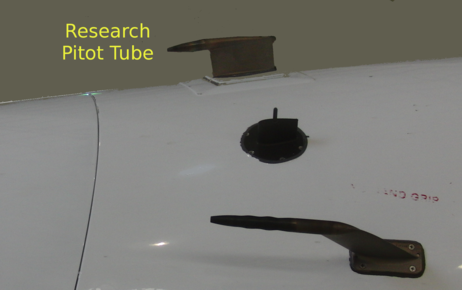
\includegraphics[width=8.5cm]{0_home_cooperw_RStudio_DEEPWAVE_WindUncertainty_PitotTube-r.png} 
\par\end{centering}

\protect\protect\protect\caption{A pitot tube used for the measurement of dynamic pressure.\label{fig:pitot-tube-photo}}
\end{figure}



\subsubsection{Airflow angles\label{sub:Airflow-angles}}

The radome gust-sensing system consists of five pressure ports\index{radome!ports}
installed in a standard GV radome\index{radome}, as shown in \index{radome!photograph}Fig.~\ref{fig:radome-photo}.
\begin{figure}
\noindent \begin{centering}
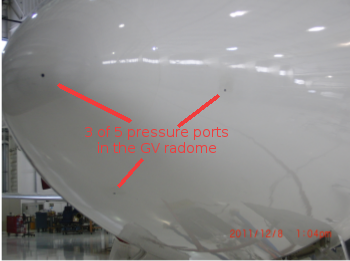
\includegraphics[width=8cm]{1_home_cooperw_RStudio_DEEPWAVE_WindUncertainty_RadomePhotoGV.png} 
\par\end{centering}

\protect\protect\caption{Photograph of the GV radome showing three of the five pressure ports
on the radome used for measurement of components of the relative wind.\label{fig:radome-photo}}
\end{figure}


The pressure ports are connected to differential pressure sensors,
one between the top and bottom ports (variable ADIFR),\sindex[var]{ADIFR=pressure difference, bottom minus top source on radome {[}hPa}\sindex[var]{BDIFR=pressure difference, starboard minus port source on radome {[}hPa{]}}
one between the left and right ports (variable BDIFR), and one between
the center port and the static source (variable QCR). The latter provides
an alternative measurement of dynamic pressure but is not normally
used. The measurements ADIFR and BDIFR are obtained from differential
pressure transducers, with characteristics\index{sensor!pressure!characteristics}
as shown in Table~\ref{tab:Radome-system-measurements}. The transducers
have specified response times of 0.05\,s and resolution 0.0015\,hPa,
with quoted stability of about 0.03\,hPa per year. These measurements
are used with procedures discussed in Section \ref{sub:radome-sensitivity}
to find the angle of attack and sideslip angle of the relative wind.
Additional information is available at \href{https://www.eol.ucar.edu/instruments/radome-gust-probe-3-d-wind-measurements}{this URL}.


\subsubsection{Components of aircraft velocity relative to the Earth}

There are two sources of information regarding the \index{speed of aircraft!ground speed}ground-speed
vector, an inertial reference unit (IRU)\index{inertial reference unit}
and a Global Positioning System (GPS).\index{Global Positioning System} 
\begin{enumerate}
\item \uline{The IRU:} The inertial system on the GV is a Honeywell\index{IRU!Honeywell!characteristics}
Laseref IV Model HG2001 GD03, with characteristics as listed in Table~\ref{tab:Radome-system-measurements}.
There are three units on the aircraft, two of which are recorded via
the ARINC data bus to standard data files. These are strap-down ring
laser gyro micro inertial systems. The measurements of ground-speed
components are affected by errors that arise from initial alignment
errors or orientation errors resulting from gyro responses to acceleration
and so often exhibit a characteristic Schuler\index{Schuler oscillation}
oscillation with magnitude that can be as much as 1--3 m\,s$^{-1}$.
This is the primary source of error in the measurements of wind, so
for aircraft velocity components it is important to remove these errors
by comparison to lower-uncertainty measurements provided by the GPS
that are not subject to the Schuler oscillation. In addition, there
are signal delays\index{GPS!delay time} that are accounted for in
post processing to align measurements with other recorded data, and
there are some inherent filters\index{IRU!filters} in the IRU computer
that affect the signals transmitted to the GV data system. The orientation\index{IRU!orientation}
of this unit was defined and checked by initial survey to coincide
with the aircraft reference axes. 
\item The \uline{GPS:} The primary GPS\index{Global Positioning System}
unit is a Novatel OEMV differential GPS unit (L1/L2) with OmniSTAR\index{OmniSTAR}
XP satellite update for ionospheric and other corrections. As used
on the GV, it reports ground-speed components at a rate of 5 Hz, although
faster rates are possible and 10\,Hz is in standard use after DEEPWAVE.
The claimed standard uncertainty\index{GPS!uncertainty} for position
is 0.15~m for vertical position; the standard uncertainty in velocity
is 0.03 m\,s$^{-1}$ when OmniSTAR corrections are available and
<0.1~m\,s$^{-1}$ otherwise.\marginpar{fix} 
\end{enumerate}

\subsubsection{Temperature\label{sub:Temperature}}

A measurement of temperature\index{temperature} is needed to calculate
the wind because the conversion from dynamic pressure to true airspeed
involves the temperature, as documented in \href{https://drive.google.com/file/d/0B1kIUH45ca5ATFV5d3QyQ0JpSjA/view?usp=sharing}{this document on processing algorithms}.\index{processing algorithms}
The measurements of temperature were checked against expectations
for height-vs-pressure changes from the hydrostatic equation by \citet{CooperEtAl2014},
with the result that the measurements were validated to an uncertainty\index{temperature!uncertainty}
of about 0.3$^{\circ}$C. Documentation of the temperature uncertainty
will be presented in more detail in a separate document.


\subsubsection{Humidity (dew point)\label{sub:dewpoint}}

\index{dew point}\index{humidity, effect of}The calculation of true
airspeed from measured dynamic and static pressure involves the specific
heats and gas constant for air, and this can depart from dry-air values
when water vapor is present in significant amounts. This correction
is usually insignificant for dew-point temperatures below about -20$^{\circ}$C
but can be important at higher dew-point temperature. The equations
used are those in \href{https://drive.google.com/file/d/0B1kIUH45ca5ATFV5d3QyQ0JpSjA/view?usp=sharing}{the document on processing algorithms}.
The correction to true airspeed is approximately a factor of (1+0.3$q_{h}$
where $q_{h}$ is the dimensionless specific humidity, typically about
0.01 at 10$^{\circ}$C dewpoint and 700~hPa pressure. In this case
the correction to airspeed, typically 150~m/s at this altitude, is
about 0.45~m/s, so the correction is not negligible but is relatively
insensitive to uncertainty in the measured humidity.The dewpoint measurements
become more uncertain than listed here at the low end of this range,
but the humidity correction is insignificant there. They are likely
better than listed here for the upper range, in level flight, but
lags and overshooting introduce errors when conditions are changing
rapidly as in climbs or descents.


\subsubsection{Examples of measurements}

\begin{figure}
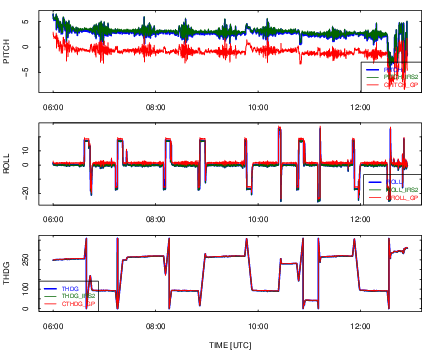
\includegraphics{2_home_cooperw_RStudio_DEEPWAVE_WindUncertainty_figure_radome-plot-angles-1.pdf}
\protect\caption[Attitude angles pitch, roll, and heading as measured by three independent
systems inertial reference units]{Attitude angles pitch, roll, and heading as measured by three independent
systems inertial reference units. The systems are: (1) the standard
Honeywell IRU (PITCH, ROLL, THDG, blue lines); (2) a duplicate backup
Honeywell IRU (PITCH\_IRS2, ROLL\_IRS2, THDG\_IRS2, green lines),
and the C-MIGITS IRU mounted in the gust pod (CPITCH\_GP, CROLL\_GP,
CTHDG\_GP, red lines). All units are degrees. Data from DEEPWAVE\index{DEEPWAVE!flight 16}
flight 16 (4 July 2014), 9:00:00 to 10:00:00\label{fig:radome-plot-angles}}
\end{figure}


\index{example of measurements!attitude angles}Typical measurements
of the attitude angles are shown in Fig.~\ref{fig:radome-plot-angles}.
The large difference in pitch is a result of the gust pod being installed
in a canister below the wing where it points downward by several degrees
relative to the aircraft longitudinal axis. (The pods were designed
this way to provide better approaching airflow for cloud-imaging probes
and other sampling from the airstream.) There is also a significant
difference in heading and in roll for similar reasons.

\begin{figure}
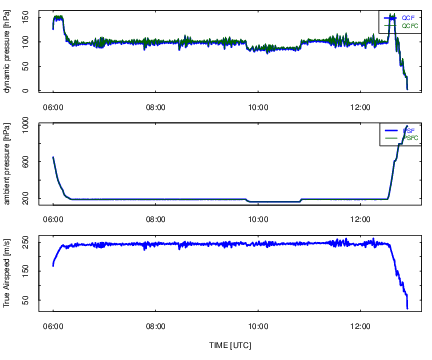
\includegraphics{3_home_cooperw_RStudio_DEEPWAVE_WindUncertainty_figure_radome-plot-pressures-1.pdf}
\protect\caption[The measurements of dynamic pressure (QCF and, after correction QCFC),
ambient pressure (PSF and corrected PSFC) and the resulting true airspeed
TASF]{The measurements of dynamic pressure (QCF and, after correction QCFC),
ambient pressure (PSF and corrected PSFC) and the resulting true airspeed
TASF. Data from DEEPWAVE\index{DEEPWAVE!flight 16} flight 16.\label{fig:radome-plot-pressures}}
\end{figure}


\index{example of measurements!pressure}\index{example of measurements!airspeed}The
measurements of pressures and the true airspeed calculated from these
measurements are shown in Fig.~\ref{fig:radome-plot-pressures} for
the same period as in the preceding figure. Corrections have been
applied to the pressure measurements according to the calibration
determined from LAMS measurements, as described by \citet{CooperEtAl2014};
these corrections vary with flight conditions but normally are smaller
than a few hPa so are not evident in these plots. They are nevertheless
crucial to reducing the uncertainty in the true airspeed to about
0.3\,m\,s$^{-1}$, as shown in that reference.

\begin{figure}
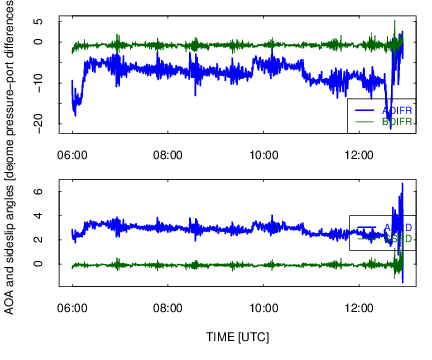
\includegraphics{4_home_cooperw_RStudio_DEEPWAVE_WindUncertainty_figure_radome-plot-airflow-angles-1.pdf}
\protect\caption[The pressure differences measured on the radome (ADIFR and BDIFR,
respectively between the vertically separated ports and the horizontally
separated ports) and the resulting airflow angles AKRD (angle of attack)
and SSRD (sideslip angle)]{The pressure differences measured on the radome (ADIFR and BDIFR,
respectively between the vertically separated ports and the horizontally
separated ports) and the resulting airflow angles AKRD (angle of attack)
and SSRD (sideslip angle). Data from DEEPWAVE\index{DEEPWAVE!flight 16}
flight 16.\label{fig:radome-plot-airflow-angles}}
\end{figure}


Figure~\ref{fig:radome-plot-airflow-angles} shows the measurements\index{example of measurements!dynamic pressure}\index{example of measurements!angle of attack}\index{example of measurements!sideslip}
of differential pressure at the radome and the resulting angle of
attack and sideslip angle calculated from those pressure differences.
The calculation is described in Section 4 of this document. Fluctuations
in sideslip angle are seldom more than a fraction of a degree, while
there can be several-degree fluctuations in the angle of attack. The
gradual decrease in angle of attack is a result of the change in fuel
load on the aircraft, which requires a smaller angle of attack to
keep the aircraft level as the weight becomes smaller.

\begin{figure}
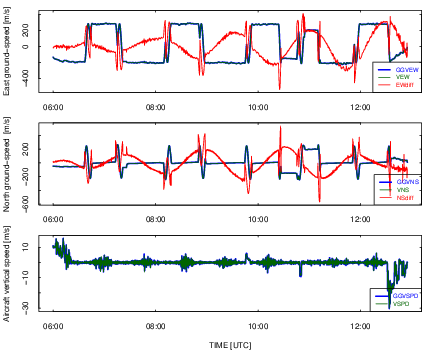
\includegraphics{5_home_cooperw_RStudio_DEEPWAVE_WindUncertainty_figure_radome-plot-groundspeed-1.pdf}
\protect\caption[Top two panels]{Top two panels: Ground-speed components as measured by the IRU and
GPS, and (red lines) the difference between the two measurements multiplied
by a factor of 100. Bottom panel: Aircraft vertical speed as measured
by the IRU (with built-in damping to the pressure altitude) and by
the GPS unit. Data from DEEPWAVE\index{DEEPWAVE!flight 16} flight
16.\label{fig:radome-plot-groundspeed}\index{example of measurements!Schuler oscillation}}
\end{figure}


The last set of components entering the measurement of wind consists
of the measurements of the motion of the aircraft with respect to
the Earth. These measurements must be combined with the measurement
of relative wind to transform the measurements to an Earth-referenced
measurement. Figure~\ref{fig:radome-plot-groundspeed} shows the
east and north components of the ground speed as measured by the IRU
and GPS. They are close enough to lie almost on top of each other
in this plot, but the red lines show the difference magnified by a
factor of 100. They clearly show the Schuler oscillation that results
from an IRU error in pitch, having magnitude of about 1--2~m\,s$^{-1}$.
This error is discussed in the next section, and Section~\ref{sub:comp-filter}
discusses how the IRU measurements (having good short-term response
but long-term drift) and the GPS measurements (having long-term accuracy
but inferior short-term response) are combined in the measurement
of wind. In addition to the Schuler oscillation, additional perturbations
associated with turns result from the mixing of pitch, roll, and heading
errors when the aircraft is banked.

\begin{figure}
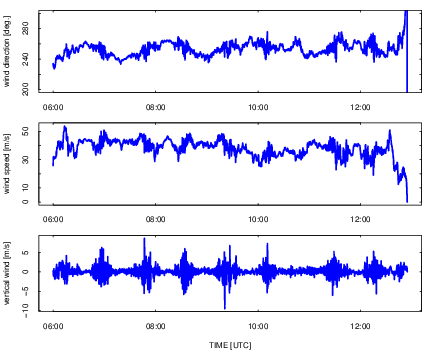
\includegraphics{6_home_cooperw_RStudio_DEEPWAVE_WindUncertainty_figure_radome-plot-wind-1.pdf}
\protect\caption{Wind measurements for DEEPWAVE\index{DEEPWAVE!flight 16} research
flight 16.\label{fig:radome-plot-wind}}
\end{figure}


\index{example of measurements!wind components}Finally, Fig.~\ref{fig:radome-plot-wind}
shows the resulting wind measurements for this flight. These measurements
will be discussed extensively in the remainder of this report, and
the uncertainty associated with them will be estimated in the closing
section.


\subsection{The gust-pod system\label{sub:The-gust-pod-system}}


\subsubsection{Overview}

The all-weather gust pod\index{gust pod}\index{all-weather wind pod|see {gust pod}}
was developed by Allen Schanot and is available for mounting under
the wing of the GV, where it was installed during the 2014 project
DEEPWAVE\index{DEEPWAVE}. It was still regarded as experimental for
that project, but performed well as documented in this document, so
it is now ready for deployment as a requestable instrument. The system
has also been called the all-weather wind pod because the primary
reason for its development was to provide a backup wind measurement
for cases when the radome system was not available, including times
when it was blocked by ice or frozen water in the pressure lines.
The gust pod fits into a standard ``PMS-style'' canister and uses
a \index{Rosemount 858 probe}Rosemount 858 probe, but the location
under the wing is one where there is substantial flow distortion\index{airflow distortion}
in comparison to the free stream so an unconventional calibration
is needed to use the measurements. The 858 probe is anti-iced by heaters
and should be unaffected by icing or ice accumulation. Five ports
are oriented forward, upward and downward 45$^{\circ}$, and left
and right 45$^{\circ}$ on the leading edge of the sensor, which has
the shape of a hemisphere. There are also ports in a ring around the
cylinder behind the hemisphere that provide a static source. The measurements
are the pressure difference between the top and bottom ports (ADIF\_GP),\sindex[var]{ADIF_GP=pressure difference between bottom and top sources, 858 
probe [hPa]@ADIF\_GP=pressure difference between bottom and top sources, 858 probe
{[}hPa{]}} the pressure difference between the right and left ports (BDIF\_GP),\sindex[var]{BDIF_GP=pressure difference between starboard and port sources, 
858 probe [hPa]@BDIF\_GP=pressure difference between starboard and port sources, 858
probe {[}hPa{]}} and the pressure difference between the forward port and the static
ports (QC\_GP).\sindex[var]{QC_GP=pressure difference between forward and static ports, 858 
probe [hPa]@QC\_GP=pressure difference between forward and static ports, 858 probe
{[}hPa{]}} In addition, the pressure provided by the ring of static ports is
recorded as PS\_GP.\index{PS_GP=pressure at static ports, 858 probe [hPa]@PS\_GP=pressure at static ports, 858 probe {[}hPa{]}}
The system incorporates a Systron Donner \index{IRU!C-MIGITS}C-MIGITS
III GPS/INS MEMS Tactical Grade navigation system (henceforth called
the C-MIGITS IRU), which is mounted in the pod to be able to measure
vibrations and wing-flex motions that will affect the measurements
of wind. This unit provides measurements of attitude angles, ground-speed
components, and accelerations and uses a GPS signal in a Kalman-filter
feedback loop to reduce errors in the measurements. The relevant specifications\index{IRU!C-MIGITS!specifications}
are listed in Table~\ref{tab:Gust-pod-measurements}.

\noindent \begin{center}
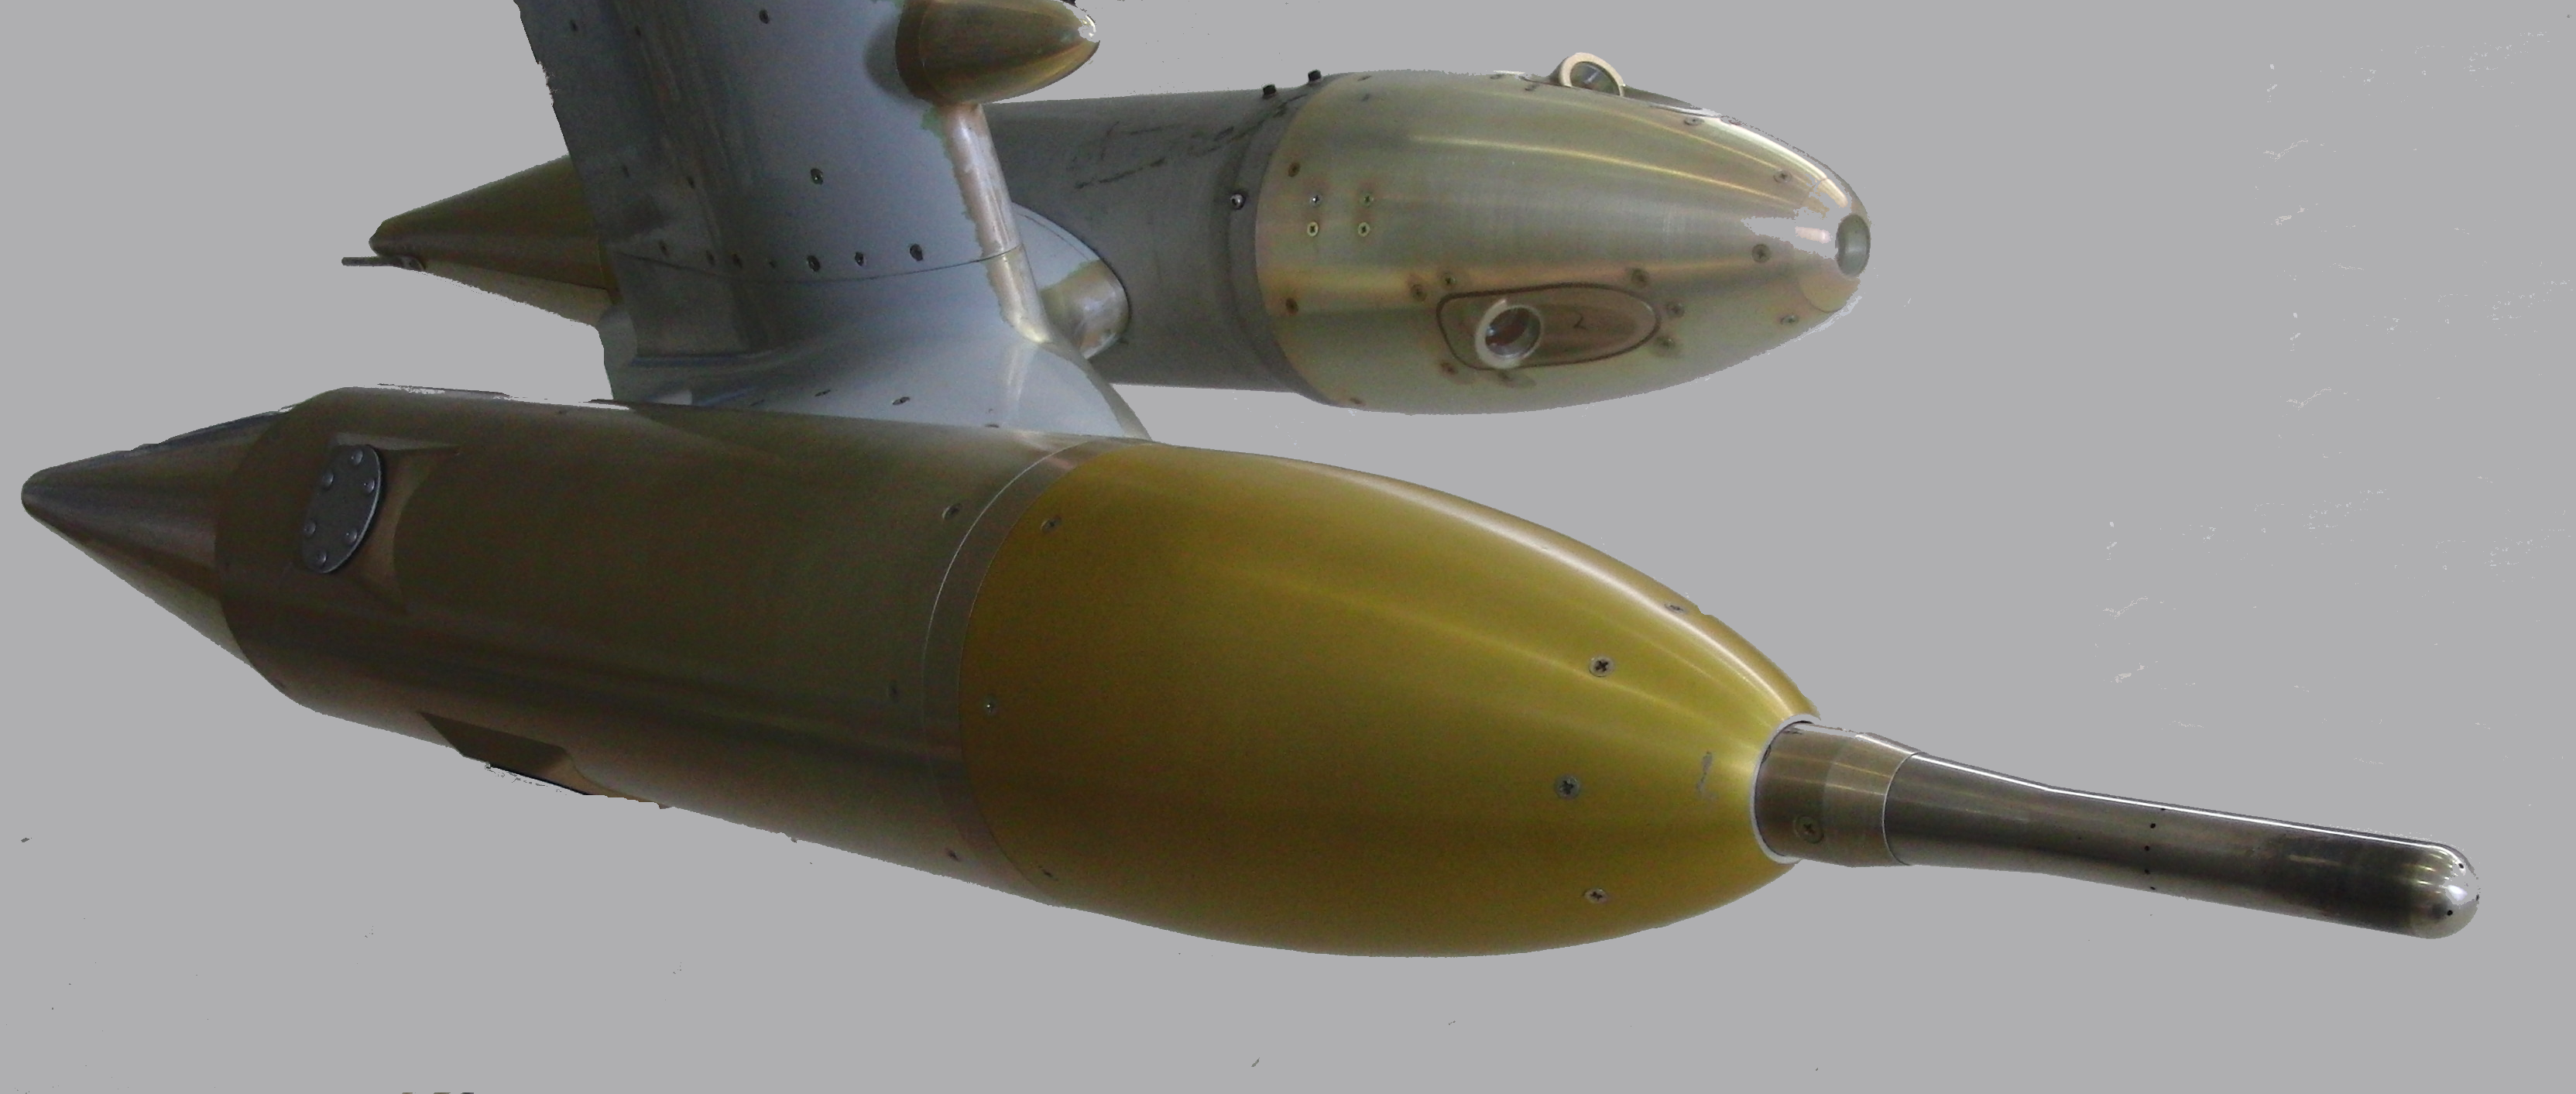
\includegraphics[width=12.1cm]{7_home_cooperw_RStudio_DEEPWAVE_WindUncertainty_GustPod1.png}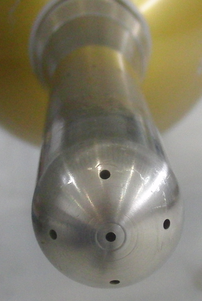
\includegraphics[height=5.1cm]{8_home_cooperw_RStudio_DEEPWAVE_WindUncertainty_GustPod2x-r.png}\\
 \textsl{Photograph of the Gust Pod (bottom left) and the ports on
the Rosemount 858 probe (right).} \index{gust pod!photograph}
\par\end{center}

\begin{table}
\begin{minipage}[t]{0.93\columnwidth}%
\begin{tabular}{>{\centering}p{2.3cm}>{\centering}p{2.7cm}>{\centering}p{2.5cm}>{\centering}p{2.2cm}>{\centering}p{2.5cm}}
\toprule 
\textbf{Measurement }\textbf{\small{}{(VARIABLE)}}{\small{} } &
\textbf{Instrument}  &
\textbf{Range, Characteristics}  &
\textbf{Standard Uncertainty}  &
\textbf{Comments}\tabularnewline
\midrule
\midrule 
velocity components (CVNS\_GP, CVEW\_GP, CVSPD\_GP)  &
C-MIGITS IRU &
with GPS  &
0.1\,m\,s$^{-1}$  &
horizontal and vertical\tabularnewline
\midrule 
pitch, roll &
 &
 &
 &
\tabularnewline
(CPITCH\_GP, CROLL\_GP)  &
C-MIGITS IRU &
with GPS  &
1\,mrad$\simeq$0.06$^{\circ}$  &
with Kalman filter \tabularnewline
\midrule 
heading &
 &
 &
 &
\tabularnewline
CTHDG\_GP  &
C-MIGITS IRU  &
with GPS  &
1.5\,mrad &
\tabularnewline
$\simeq$0.09$^{\circ}$  &
valid when in motion\footnote{Without occasional turns the heading error grows linearly at about
1--10$^{\circ}$/hour} &
 &
 &
\tabularnewline
\midrule 
pressure differences,858 ports &
 &
 &
 &
\tabularnewline
(ADIFR\_GP, BDIFR\_GP)  &
Honeywell PPT0001-DXX2VB-S021  &
$\pm1$ psi$\simeq$$\pm$68.95 hPa  &
0.07 hPa &
\tabularnewline
0.14 hPa max.  &
the first is ``typ.''; same transducers as for radome &
 &
 &
\tabularnewline
\midrule 
dynamic pressure (QC\_GP)  &
Honeywell PPT0005-DXX2VB-S021 &
0--5 psi $\simeq$0--345 hPa  &
0.17 hPa &
\tabularnewline
0.34 hPa max.  &
`` &
 &
 &
\tabularnewline
\midrule 
ambient pressure (PS\_GP)  &
Paroscientific 6000-15A-28  &
0--15 psi $\simeq$0--1035\,hPa  &
0.10\,hPa  &
digital transducer\tabularnewline
\bottomrule
\end{tabular}%
\end{minipage}

\protect\protect\caption{Characteristics of measurements from the gust-pod that are used for
the calculation of the wind. There is further discussion of each measurement
in the text of Sect.~\ref{sub:The-gust-pod-system}.\label{tab:Gust-pod-measurements}\index{specifications!gust pod}}
\end{table}



\subsubsection{Attitude angles}

\index{angle!attitude!gust pod}\index{gust pod!components}The C-MIGITS
IRU unit provides measurements of the attitude angles, recorded as
variables CROLL\_GP, CPITCH\_GP, and CTHDG\_GP. The estimated standard
uncertainty\index{IRU!CMIGITS!uncertainty} in measurement of pitch,
1~mrad (cf.~Table~\ref{tab:Gust-pod-measurements}), is supported
by comparison to the cabin-mounted inertial systems; the standard
deviation in the difference between the two systems was about 0.1$^{\circ}\simeq1.7$~mrad
for extensive multi-flight comparisons, while the expected difference
for two systems each having standard uncertainties of 1 mrad would
be 1.4\,mrad. Some contribution would be expected from vibrations
and wing flex that affect the gust pod, so these comparisons are good
support for the approximate validity of the specifications. However,
the feedback from the Kalman filter using GPS measurements can be
ineffective in the absence of turns or maneuvers, so some of the specified
uncertainties, esp.~for heading, can be exceeded significantly in
the absence of maneuvers, as noted in Table~\ref{tab:Gust-pod-measurements}.


\subsubsection{Ambient or static pressure}

\index{pressure!ambient!gust pod}\index{gust pod!components}Ambient
pressure (variable PS\_GP) is measured by a digital transducer with
low uncertainty, as listed in Table~Table~\ref{tab:Gust-pod-measurements}.
However, the Rosemount 858 probe is located under the wing in a location
where there is significant airflow distortion, so these measurements
often differ from the measurements from the static buttons on the
fuselage by 10--20\,hPa and significant corrections are needed if
these measurements are to be used for pressure measurements. With
the gust-pod, the use is as a reference for the differential measurement
of dynamic pressure because the dynamic-pressure transducer is connected
between the total-pressure port on the front of the 858 probe and
the static ports. No calibration has been determined that would make
this measurement useful as a measure of true ambient pressure, although
that could be done by fitting to match the standard static pressure.
In the absence of such a correction, PS\_GP should not be considered
an alternate measurement of ambient pressure. The use of this measurement
to determine an alternate measure of true airspeed will be discussed
in Section~\ref{sub:GP-TAS}.


\subsubsection{Dynamic pressure}

\index{pressure!dynamic!gust pod}\index{gust pod!components}The
dynamic pressure QC\_GP is measured by a differential pressure transducer,
with characteristics shown in Table~\ref{tab:Gust-pod-measurements}.
The measurement is the pressure difference between the forward-pointing
port on the Rosemount 858 probe and the static ports on the side of
that probe. Because the system is located under the wing in a region
of disturbed airflow, the dynamic pressure requires unconventional
correction to obtain the airspeed, as discussed in Sect.~\ref{sec:Calibrations}.
This measurement is also used in the calculation of flow angles from
the gust-pod pressure ports, as also discussed in that section.


\subsubsection{Airflow angles}

\index{angle!airflow!gust pod}The difference between pressures at
the top and bottom ports of the Rosemount 858 probe (ADIFR\_GP) and
the corresponding difference between right and left ports (BDIFR\_GP)
are also measured using differential transducers listed in Table~\ref{tab:Gust-pod-measurements}.
These are digital transducers that produce output with a fixed relationship
to the pressure differences, and those digital outputs are recorded
by the aircraft data system.


\subsubsection{Components of aircraft velocity relative to the Earth}

The C-MIGITS\index{IRU!C-MIGITS} IRU, mounted with the gust pod,
provides digital representations of the ground-speed components CVEW\_GP
and CVNS\_GP and the vertical speed CVSPD\_GP. (cf.~Table~\ref{tab:Gust-pod-measurements}).
The unit incorporates a GPS\index{Global Positioning System} receiver
and uses GPS information as input to a Kalman filter\index{filter!Kalman}
for adjustment of these measurements and others discussed in this
section.


\subsubsection{Temperature and humidity}

Air temperature and dew point are measured in the same way as discussed
for the radome system in Sects.~\ref{sub:Temperature} and \ref{sub:dewpoint},
and the same variables (ATX and DPX) are used.


\subsubsection{Examples of measurements}

A new calibration is developed in Section \ref{sec:Calibrations}.
On the basis of that new calibration, it appears that the gust pod
provides a useful alternative to wind measurements based on the radome.
Plots and average values are presented there to support the validity
of this measurement.\index{example of measurements!gust pod}

% For coding of the processing and construction of the plots used here,% see the file \textasciitilde{}cooperw/ RStudio/DEEPWAVE/GustPodProcessor.Rnw% on EOL file systems. This program, if run from within the html interface% to RStudio on tikal using the \textquotedbl{}Compile PDF\textquotedbl{}% function, will produce this section of the current document while% processing a netCDF file to add new gust-probe variables to it. The% processor also attempts to flag bad CTHDG\_GP measurements, which% apparently occur as the heading moves through 180 deg. (This would% be better replaced by interpolation at these points.)

%For similar%results from DEEPWAVE rf05, saved for reference, see GPcal.pdf, a%note saved on 22 June 2014.\marginpar{XXX}

\begin{figure}
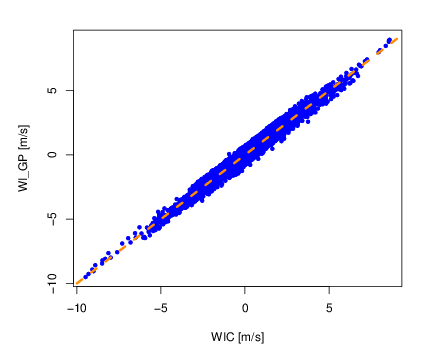
\includegraphics{9_home_cooperw_RStudio_DEEPWAVE_WindUncertainty_figure_vw-gp-vs-wic-1.pdf}
\protect\caption{Comparison of vertical wind calculated from the gust pod (WI\_GP)
to the conventional measurement of vertical wind (WIC). The dashed
orange line is a 1:1 reference line, and each blue dot represents
a 1-s pair of corresponding measurements.\label{fig:vw-gp-vs-wic}\index{wind!vertical!gust pod}}
\end{figure}


\begin{figure}
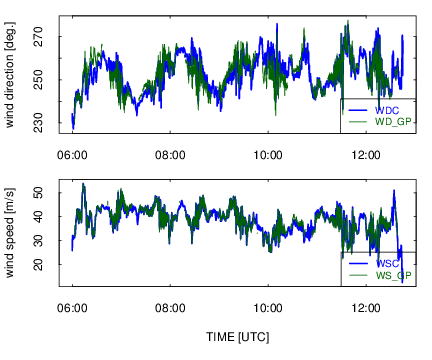
\includegraphics{10_home_cooperw_RStudio_DEEPWAVE_WindUncertainty_figure_hw-gp-vs-std-1.pdf}
\protect\caption{Comparison of horizontal wind direction (top panel) and horizontal
wind speed (bottom panel) as determined from the gust pod and from
the conventional radome-based system, for measurements where the true
airspeed is greater than 130 m/s (to exclude periods of possible flap
deployment). Only measurements considered valid are plotted for the
gust pod; the restrictions where the gust-pod measurement is flagged
as missing and therefore is not plotted here are: altitude (GGALT)
> 5000 m, absolute value of roll (ROLL) < 5$^{\circ}$. This causes
exclusion of some measurements near the start and end of the flight
and during turns.\label{fig:hw-gp-vs-std}\index{wind!horizontal!gust pod}}
\end{figure}


The following are some plots that show the results of this processing,
in this case from DEEPWAVE\index{DEEPWAVE!flight 16} flight RF16
on 4 July 2014. Figure~\ref{fig:vw-gp-vs-wic} shows a comparison
of the vertical wind calculated from the gust pod (WI\_GP) vs the
conventional vertical wind (WIC). The standard deviation between the
two measurements is 0.27\,m/s. % mean diff 0.13This is a good illustration
of performance because this is a flight with large-amplitude waves
and some of the largest vertical-wind measurements in the DEEPWAVE
project, so the consistency of these measurements even to extremes
in this plot indicates that the measurements from the gust pod are
useful even for these large-amplitude measurements. Figure~\ref{fig:hw-gp-vs-std}\index{wind!vertical!gust pod}
shows the corresponding horizontal-wind measurements, and also shows
good agreement between the gust pod and the conventional wind-sensing
system.\footnote{Some spikes would occur in turns if the exclusions listed in the figure
caption were not applied to the measurements from the gust pod. These
are the result of a problem with the C-MIGITS IRU measurement of heading,
which exhibits noisy fluctuations as it moves through 180$^{\circ}$.
These fluctuations introduce large perturbations in the horizontal
wind measurements, affecting esp.~the east component of the wind.}

\begin{figure}
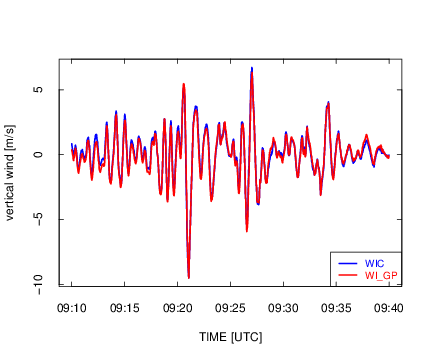
\includegraphics{11_home_cooperw_RStudio_DEEPWAVE_WindUncertainty_figure_vw-gp-small-segment-1.pdf}
\protect\caption{A 30-min segment from flight 16 of the DEEPWAVE\index{DEEPWAVE!flight 16}
project, showing the good agreement of the vertical wind measurements
from the gust pod (WI\_GP) and from the conventional wind-sensing
system on the GV (WIC).\label{fig:vw-gp-small-segment}}
\end{figure}


A small segment of flight from a period with large-amplitude waves
is shown in Fig.~\ref{fig:vw-gp-small-segment}. The two measurements
match quite well in regard to the structure of these waves and the
amplitudes of the fluctuations. The measurements of horizontal wind
speed are in similar agreement, but the wind direction for this period
shows an offset for the gust pod measurement relative to the conventional
measurement, varying from about 5$^{\circ}$ near the start of this
period to about 1$^{\circ}$ near the end. This is a result of an
apparent error in heading from the C-MIGITS IRU, a common feature
to see near the start of flights but one that usually was made smaller
during flight by the action of the GPS updating via Kalman filter
in that unit.

The result of this error in wind direction and the problems with measured
heading for flight exactly southbound complicate the use of the measurements
of horizontal wind from the gust pod and make them of lesser quality
that the standard measurements. Fortunately, in this and most projects,
the horizontal-wind measurements are available from the radome-based
system on all flights and are usually not compromised even when there
is loss of the measurement of angle of attack from plugging of the
lines in the radome, because the side-mounted ports for the measurement
of sideslip seldom are plugged.

% \begin{figure}% {\centering \includegraphics[width=300pt]{figure/Plotted-Results1}% % }% % \protect\protect\caption[WIG (vertical wind based on the gust pod) plotted against WIC (vertical% wind from the conventional radome-based gust system)]{WIG (vertical wind based on the gust pod) plotted against WIC (vertical% wind from the conventional radome-based gust system)\label{fig:Plotted-Results1}}% \end{figure}% % % \begin{figure}% {\centering \includegraphics[width=300pt]{figure/Plotted-Results2}% % }% % \protect\protect\caption[Angle of attack determined from gust-pod measurements, plotted vs]{Angle of attack determined from gust-pod measurements, plotted vs.% corresponding measurements AKRD from the standard wind sensing system\label{fig:Plotted-Results2}}% \end{figure}% % % \begin{figure}% {\centering \includegraphics[width=300pt]{figure/Plotted-Results3}% % }% % \protect\protect\caption[Comparison of horizontal wind measurements from the gust pod (red% lines) and from the standard wind measurements WDC and WSC (thicker% blue lines)]{Comparison of horizontal wind measurements from the gust pod (red% lines) and from the standard wind measurements WDC and WSC (thicker% blue lines).\label{fig:Plotted-Results3}}% \end{figure}% % % \begin{figure}% {\centering \includegraphics[width=300pt]{figure/Plotted-Results4}% % }% % \protect\protect\caption[Comparison of vertical wind measurements from the gust pod (red line)% and from the standard wind measurement (WIC, blue line)]{Comparison of vertical wind measurements from the gust pod (red line)% and from the standard wind measurement (WIC, blue line).\label{fig:Plotted-Results4}}% \end{figure}% % % \begin{figure}% \noindent \begin{centering}% \includegraphics[width=10cm]{GPrf11Fig1} % \par\end{centering}% % \protect\protect\protect\caption{\label{fig:3panelHWVW}A comparison between the conventional wind% components (blue lines) and the wind from the gust pod (red lines).% Data from flight RF05.}% \end{figure}% % % Some plots showing the nature of the new variables (WDG, WSG, WIG)% are included here. The first one (Fig.~\ref{fig:3panelHWVW}) shows% a comparison of all three wind variables for a segment from flight% RF11. The spike in WSG at about 9:43 has a known origin and will be% removed. There is also a short period near 9:23 when the vertical% wind measurements appear offset by a few tenths m\,s$^{-1}$. Otherwise, the% gust pod provides a good representation of the standard variables.% \begin{figure}% \noindent \begin{centering}% \includegraphics[width=10cm]{GPrf11Fig2} % \par\end{centering}% % \protect\protect\protect\caption{\label{fig:ExpandedViewF1}An expanded view of a section of Fig.~\ref{fig:3panelHWVW}.}% \end{figure}% % % Figure \ref{fig:ExpandedViewF1} shows an expanded view and emphasizes% the small difference between wind speeds from the two systems; this% is likely caused by IRU differences and can later be improved by reference% to the GPS signals with OMNISTAR. The similarities and differences% in WIG vs WIC are also more evident in this figure.

\begin{figure}
\noindent \begin{centering}
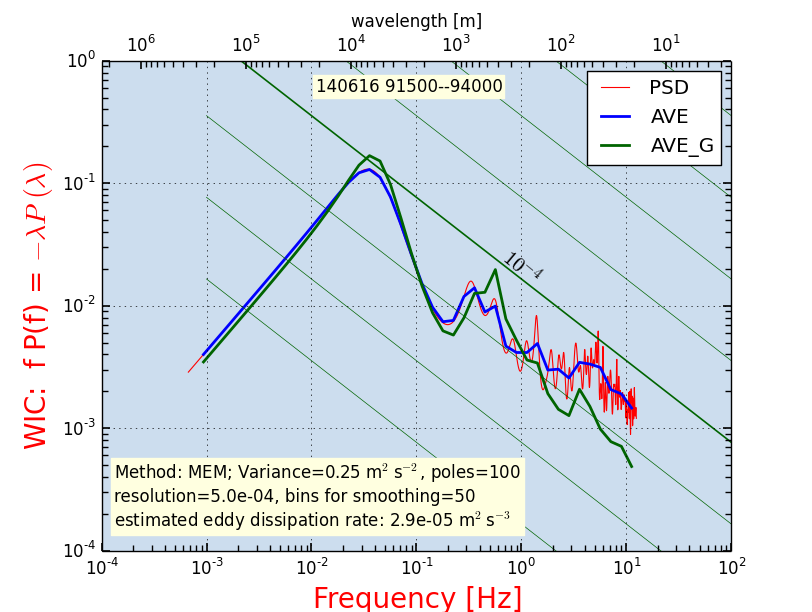
\includegraphics[width=10cm]{12_home_cooperw_RStudio_DEEPWAVE_WindUncertainty_GPrf11Fig5.png} 
\par\end{centering}

\protect\protect\protect\protect\caption{\label{fig:VarSpecWICandWIG}Variance spectra for WIC (red line labeled
PSD, unsmoothed, and also shown smoothed as the blue line), compared
to the smoothed spectrum for WIG from the gust pod (green line). Data
from flight RF05, 9:15:00--9:40:00.\index{variance spectrum!vertical wind!gust pod}\index{power spectrum|see {variance spectrum}}}
\end{figure}


Figure \ref{fig:VarSpecWICandWIG} shows the high-rate variance spectra
from the two systems. There is a significant difference at frequencies
above about 3 Hz, with the gust-pod distribution dropping faster and
the standard wind WIC showing more variance. The high frequency spectrum
from the gust pod may be more realistic; it is unusual to see high
variance at these frequencies without a related generating source.
The coherence between the radome and gust-pod measurements was above
0.9 for frequencies less than 1 Hz but then fell to around 0.2 at
10 Hz. This is an indication that the two measurements are different
in important ways at high frequency. This would not be the case if
they were responding with different amplitudes; the signals must really
be mostly incoherent at the highest frequency. The separation wing-to-fuselage
is about 7 m lateral and 13 m longitudinal, so that doesn't seem enough
to cause the low high-frequency coherence. The phase changes from
in-phase at frequencies less than 1 Hz to 180$^{\circ}$ out-of-phase
at 9 Hz, with WIG lagging, so this is consistent with the longitudinal
offset. Shifting WIG relative to WIC also gave maximum coherence when
WIG was shifted forward 1/25 s. Figure~\ref{fig:FurtherExpandedWIGshifted}
shows an example of the good correspondence between gust-pod and radome
measurements of vertical wind after application of such a shift to
25-Hz measurements.

\begin{figure}
\noindent \begin{centering}
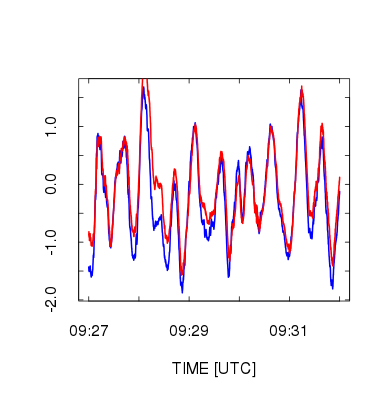
\includegraphics[width=10cm]{13_home_cooperw_RStudio_DEEPWAVE_WindUncertainty_GPrf11WIGshiftM1.png} 
\par\end{centering}

\protect\protect\protect\protect\caption{\label{fig:FurtherExpandedWIGshifted}Comparison of WIG (red line)
and WIC (blue line) after shifting WIG 1/25 s earlier to compensate
for the longitudinal displacement of the sensor.}
\end{figure}



\subsubsection{Mixing of Attitude Angles for the Gust Pod}

% The gust pod does not yet perform well% in turns. The reason is that the gust-pod IRU is oriented to point a few degrees from% the longitudinal axis of the aircraft, and as% a result any roll of the aircraft introduces complex combinations% of roll, heading, and pitch into the gust-pod IRU. It should be possible% to remove these to some extent, but a procedure for correction of the% angles in turns has not yet been developed or implemented.

% The circle maneuvers% from the calibration flight should provide valuable information regarding% the potential for improving the in-turn performance of the gust pod.

\index{gust pod!problem in turns}The attitude angles (pitch, roll,
heading) as measured by the gust-pod IRU are defined relative to the
orientation of the inertial unit in the gust pod, which is aligned
a few degrees from the longitudinal axis of the aircraft. The canisters
on the GV are oriented with axis pointing inward and downward relative
to the aircraft longitudinal axis, in order to align with normal airflow
at the pods. This is desirable for hydrometeor sampling and minimum
drag, but it complicates the calculation of wind because roll introduced
in turns, primarily a rotation about the aircraft longitudinal axis,
will appear as a combination of attitude-angle changes in the gust
pod. Errors arising from the initial alignment at the start of flights
will also cause problems with the measured attitude angles, and it
is likely that these will be more significant near the start of flights
because the built-in Kalman filter uses GPS measurements to correct
such errors in the course of the flight.

This problem with the reference frame for attitude angles has two
consequences: 
\begin{enumerate}
\item Measurements from the gust pod in turns have large errors in comparison
to the errors in level flight. The measurements from the gust pod
should probably be flagged as of poor quality whenever the roll exceeds
some threshold like perhaps $\pm5^{\circ}$. The measurements usually
look reasonable in turns despite this worry, but the largest errors
occur there. 
\item There may be an offset introduced by the mixing of sideslip and angle
of attack, arising from the difference in roll angle, and this will
affect the reference or average value of the measured vertical wind.
Some flights (e.g., DEEPWAVE\index{DEEPWAVE!flight 18} flight 18)
have a significant offset in vertical wind from the gust pod at the
start of the flight that is related to offsets in heading and roll,
gradually corrected in the course of the flight via the C-MIGITSIII
IRU Kalman filter. 
\end{enumerate}
Because the weight of the aircraft decreases during the flight, so
does the angle of attack. When the wing flexes, the measured sideslip
at the gust pod also varies with weight of the aircraft. This change
in sideslip causes an offset in the mean lateral component of the
wind as measured by the gust-pod system.

% as shown by Fig.~\ref{fig:SSGPrf18}, so there will be an offset% in sideslip that will affect the mean lateral component of the wind.% \begin{figure}% \noindent \begin{centering}% \includegraphics[width=10cm]{GPF1} % \par\end{centering}% % \protect\protect\protect\caption{\label{fig:AOAGPrf18}Angle of attack measured by the gust-pod system% on DEEPWAVE flight RF18.}% \end{figure}% % % \begin{figure}% \noindent \begin{centering}% \includegraphics[width=10cm]{GPF2RF18} % \par\end{centering}% % \protect\protect\protect\caption{\label{fig:SSGPrf18}Sideslip angle measured by the gust-pod system% on DEEPWAVE flight RF18.}% \end{figure}% % % In addition, this flight had a particularly large offset in the vertical% wind from the gust pod (WIG) at the start of the flight, as shown% in % \begin{figure}% \noindent \begin{centering}% \includegraphics[width=10cm]{GPF3} % \par\end{centering}% % \protect\protect\protect\caption{\label{fig:WIGoffset}The vertical wind determined by the gust pod% (WIG) and via standard processing (WIX, to distinguish this from WIC% as determined by erronous in-field processing), for flight RF18 of% the DEEPWAVE project.}% \end{figure}% % % Fig.~\ref{fig:WIGoffset}. This offset is associated with a brief% period where the difference in heading between the IRU in the gust% pod and that in the fuselage were unusually large, as shown in % \begin{figure}% \noindent \begin{centering}% \includegraphics[width=10cm]{GPF4} % \par\end{centering}% % \protect\protect\protect\caption{\label{fig:HDGerror}The difference in heading between the values% measured by the IRU in the gust pod and the IRU in the cabin, for% DEEPWAVE flight RF18.}% \end{figure}% % % Fig.~\ref{fig:HDGerror}. In addition, the mean value of the measured% roll was close to zero for the in-cabin IRU but about 1.375$^{\circ}$% for the gust-pod IRU. Coupling among these attitude angles appears% to have caused the large offset in WIG at the start of this flight.% Because the gust-pod IRU incorporates a Kalman filter that can use% measured errors in position and ground speed as determined by comparison% to a GPS measurement to refine the measurements, the large error appears% to have been corrected as the flight progressed.

These effects suggest that the vertical wind measured by the gust
pod may have an offset in some cases, particularly at the start of
flights, and the measurement of sideslip can also have an offset that
will contribute to the lateral component of the measured wind. These
are weaknesses in the measurements from the gust pod that, at this
stage, do not appear easily corrected. A future study implementing
Schuler tuning in a post-processing step and correcting for the entwined-angle
effects may be able to reduce these weaknesses, but that will require
continued analysis not performed for this report.\marginpar{XXX}
It may also be possible to develop special processing that corrects
the measurement of attitude angles in turns, but that has not yet
been developed or implemented.

% % \subsubsection{Next Steps}% \begin{enumerate}% \item A procedure for processing the gust-pod measurements will be needed.% It may be possible to use code in gusto.c for this purpose or otherwise% to implement the process used here into nimbus, because this is being% done second-by-second as needed for nimbus. Alternately, the code% used here can run after nimbus processing to add the gust-pod variables.% If this course is followed, the R script could be improved because% I didn't vectorize the angle transformations yet, in the interest% of getting it to work first. The software / data processing group% will have to decide which is better, and it may be preferable to use% different procedures for DEEPWAVE and for future use in order to produce% the DEEPWAVE data quickly. % \item As noted above, there are issues with the gust-pod measurements in% turns that need to be addressed. These issues will affect the standard% data also because in turbulence the roll changes and this may feed% into the other measurements even at small roll angles. % \item The relative timing of the measurements entering the calculation of% wind still needs to be addressed. The IRU information is transmitted% for recording with some delay, and corrections for those delays are% in place. However, small errors in those delays can cause phase shifts% among the measurements that, for example, result in residual perturbations% of the vertical wind during pitch maneuvers. These should be tuned% to minimize those perturbations. % \item An additional worthwhile study will be to see if using GPS measurements% to determine the Schuler oscillation can improve measurements of pitch% and heading and so lead to improved wind measurements. There is some% evidence of this problem in an apparent changing offset in the vertical% wind, so any improvement here can be very useful to DEEPWAVE. \end{enumerate}


\subsection{The laser air-motion sensor\label{sub:LAMS-description}}

The laser air-motion sensor (LAMS)\index{laser air-motion sensor}
is still under development so results presented here will be less
extensive than for the other systems. The characteristics and associated
uncertainties in measured wind are discussed by \citet{SpulerEtAl2011}
and \citet{CooperEtAl2014}. Figure~\ref{fig:LAMSschematic} shows
the one-beam LAMS as installed on the GV, and Fig.~\ref{fig:LAMS-4Beam}
shows the configuration of the three or four-beam version.\index{LAMS!schematic} 

\noindent \begin{center}
\begin{figure}
\noindent \centering{}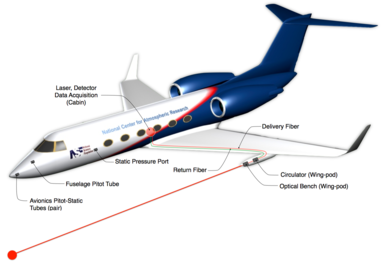
\includegraphics[width=0.9\columnwidth]{14_home_cooperw_RStudio_DEEPWAVE_WindUncertainty_amt-2014-0031-f01-r.pdf}\protect\caption{Diagram of the LAMS. Light generated by the laser in the cabin is
transmitted by optical fibres to a~wing pod, where it is transmitted
in a beam that has a~focal point well ahead of the aircraft (farther
ahead than suggested by this not-to-scale diagram). The light backscattered
from aerosol particles in the focal region is collected by the lens,
and a circulator mixes a~portion of the transmitted signal with the
returned signal. The resulting signal, with interference patterns
that measure the Doppler shift of the backscattered light, is returned
via optical fibre to the cabin for digitization. Also illustrated
in this figure are the approximate locations of the static pressure
ports and the fuselage pitot tube used by the research data system
to measure static and dynamic pressures. This figure appears in Applied
Optics in the article by \citet{SpulerEtAl2011} and is used here
with permission from the Optical Society of America.\label{fig:LAMSschematic}}
\end{figure}

\par\end{center}

\noindent \begin{center}
\begin{figure}
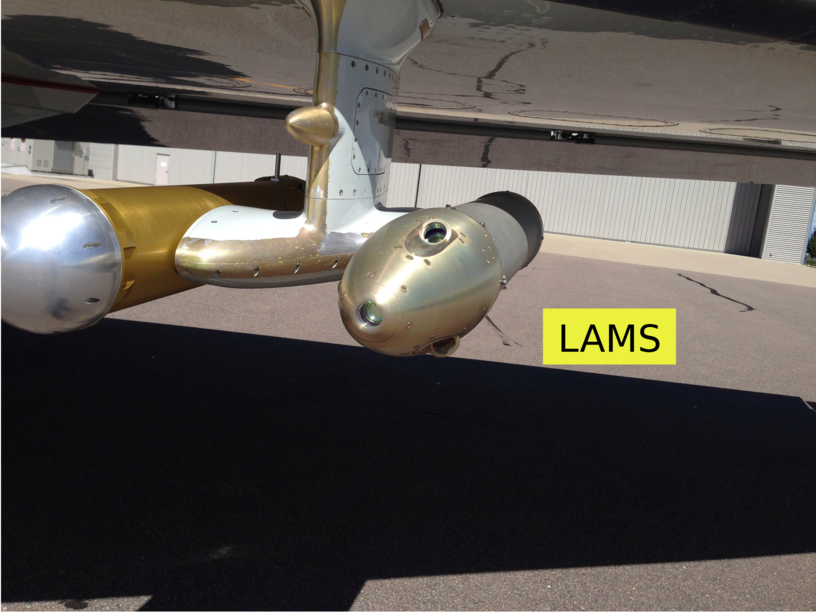
\includegraphics[width=0.59\columnwidth]{15_home_cooperw_RStudio_DEEPWAVE_WindUncertainty_LAMS-1r.png}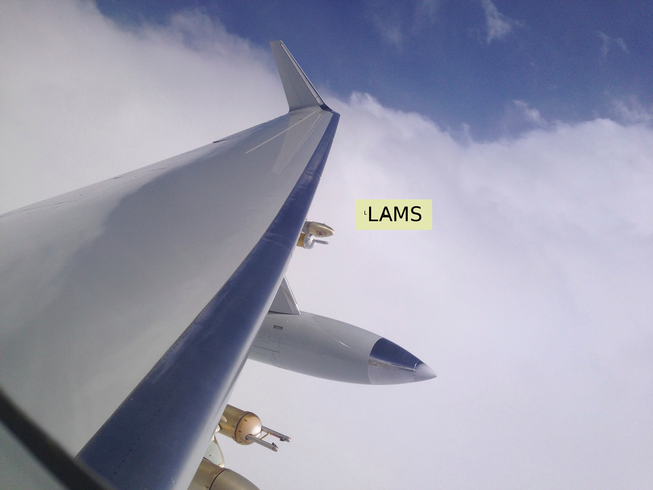
\includegraphics[width=0.4\columnwidth]{16_home_cooperw_RStudio_DEEPWAVE_WindUncertainty_LAMS-2r.png}\protect\caption{The four-beam configuration of the LAMS optical head as installed
in a GV under-wing pod.}
\label{fig:LAMS-4Beam}\index{LAMS!photograph}
\end{figure}

\par\end{center}

The system consists of one, three or four fiber-based laser beams
focused ahead of the aircraft and a collection system to detect the
Doppler shift in light backscattered from aerosols. The transmitter
optical components are mounted in an underwing pod, similar to that
used for the gust pod, and like the gust pod the system incorporates
a compact \index{IRU!LAMS}\index{IRU!SDN500}Systron Donner SDN500
GPS/INS MEMS Tactical Grade navigation system (henceforth called the
SDN500 IRU) to measure the attitude angles and ground speed of the
pod. Early measurements from this system have been used to determine
corrections to the pressure measurements, and those serve an important
role in reducing uncertainty in the wind measurements, as described
in \citet{CooperEtAl2014} and later in this report.

LAMS\index{LAMS!4-beam configuration} hardware supports up to four
beams, with three pointing $35^{\circ}$ off the forward direction,
with $120^{\circ}$ separation about the azimuthal direction. The
fourth beam is directed forward from the LAMS unit. The LAMS\index{LAMS!in DEEPWAVE}
channel designations changed after DEEPWAVE (summer 2014) when it
was decided the instrument would benefit from having a lower noise
channel for forward pointing measurements (the laser/detector on channel
4 had lower SNR than the other three channels). Table \ref{tab:BeamConfig}
summarizes the labels and pointing angles of each beam for both up
to and after DEEPWAVE. Note the number designation refers to the laser,
detector, and data processing channels. The letter designation is
associated with the exit window on the LAMS head. The pointing angles
reported here are ideal. The angle $\theta$ is measured relative
to the forward direction of the LAMS pod (approximately the angle
between the beam and $\hat{x^{\prime}}$) and the angle $\phi$ is
the rotation angle about $\hat{x^{\prime}}$ relative to the $\hat{z^{\prime}}$
axis. This geometry is designed for GV installation where the LAMS
pod is installed on the left wing, outboard pylon, outboard position.
The pointing geometry relative to the aircraft may change based on
the installation configuration on the C-130 (to be determined on ARISTO
in fall 2015) where the LAMS optical fiber are routed to the aircraft
right wing.

\begin{table}
\begin{minipage}[t]{0.93\columnwidth}%
\begin{center}
\begin{tabular}{>{\centering}p{3.5cm}>{\centering}p{3.5cm}>{\centering}p{2.5cm}>{\centering}p{2.5cm}}
\toprule 
\textbf{Beam Name} &
\textbf{Beam Name} &
 &
\tabularnewline
After DEEPWAVE &
Before/During DEEPWAVE &
\textbf{$\theta_{L}$}  &
\textbf{$\phi_{L}$} \tabularnewline
\midrule 
Beam 1/A  &
Beam 1/A  &
$35^{\circ}$  &
$180^{\circ}$ \tabularnewline
\midrule 
Beam 4/B  &
Beam 2/B  &
$35^{\circ}$  &
$60^{\circ}$ \tabularnewline
\midrule 
Beam 3/C  &
Beam 3/C  &
$35^{\circ}$  &
$-60^{\circ}$ \tabularnewline
\midrule 
Beam 2/D  &
Beam 4/D  &
$0^{\circ}$  &
-- \tabularnewline
\bottomrule
\end{tabular}
\par\end{center}%
\end{minipage}\protect\caption{Designations and ideal orientations of LAMS beams for installation
on the GV. $\theta_{L}$ is the angle from the longitudinal axis of
the aircraft to the beam, and $\phi_{L}$ is the azimuthal angle of
rotation about the longitudinal axis relative to the downward (aircraft-axis)
direction, with positive values to starboard. In particular, beam
1 is upward at an angle of 35$^{\circ}$ from the centerline of the
aircraft.\label{tab:BeamConfig}\index{LAMS!pointing angles}}
\end{table}


During IDEAS-4-GV, the LAMS beams\index{LAMS!focal distance} were
focused approximately 15 m from the LAMS exit ports on the pod. After
this flight program, concerns were raised about the aircraft causing
\index{LAMS!airflow distortion}flow distortion in the LAMS sample
volumes, and the beam focus was moved to 20 m from the exit port.
In both cases the sample volume is approximately 2 m long.


\subsubsection{Relative Beam Pointing}

The relative pointing of the LAMS beams is defined by the orientation
of each beam relative to the others. If the absolute pointing direction
of one beam is known, the relative pointing may be used to determine
the absolute pointing of all other beams. We define the relative pointing
coordinates such that the z-axis is directed along the forward beam
(D). The angle $\theta_{L}$ is the angle between the beam and the
z-axis and the azimuthal angle $\phi_{L}$ is measured relative to
the x-axis such that beam 1 (A) is positioned at $\phi_{L}=0$.\sindex[lis]{phi\_subL@$\phi_{L}$=LAMS azimuthal pointing angle}\sindex[lis]{theta\_subL@$\theta_{L}$=LAMS pointing angle from longitudinal axis}

Two methods were used to determine the relative pointing angles. The
first, performed prior to IDEAS-4-GV, used a Laser Survey, in which
a commercial laser surveying\index{LAMS!pointing angles!survey} company
measured the positions of the LAMS head and the beam focal points.

The second method used a 30x beam expanded with focusing lens in a
fixed position (referred to here as the receiver system) while LAMS
was mounted in an astronomical telescope mount. A camera was placed
at the focal point of the receiver system and the telescope mount
was used to steer the LAMS beams into the receiver system such that
each beam was centered on the CCD. This method had redundant pointing
measurements, using both SDN500 data as well as the telescope mount
angle read-outs.

Both methods were relatively accurate, with less than $0.2^{\circ}$
difference in beam pointing. It should be noted that the fibers on
the LAMS head may have moved slightly between the two measurement
methods. The forward pointing beam was added after IDEAS-4-GV which
required some disassembly of the LAMS head. So the relatively small
difference in beam pointing may be partially attributable to that
work.

%The beam pointing results from the telescope measurement system are typically used going forward, first because they are the most recent beam pointing measurements, but also because redundant measurements and the position invariance of Fourier plane measurements generally illicit greater confidence in those pointing results.

%\subsubsubsection{Laser Survey}

Prior to IDEAS-4-GV in Sept.--Oct.~2013, a laser survey system was
used to estimate the LAMS beam pointing angles of Beams 1, 2, and
3 (the forward pointing beam had not been added at that point). The
LAMS head was positioned in the hanger so the bottom two beams were
approximately parallel to the floor. Two IR card targets were placed
at the focal points of those beams.

The laser survey system locked onto a corner cube reflector and register
its position in space. The corner cube was first used to estimate
the position of the LAMS exit ports by taking a series of points around
their circumference. The tracker then registered the positions of
the IR card targets by the same method. Once complete, the LAMS head
was rotated by $120^{\circ}$ and the process was repeated. This measurement
was repeated for three different LAMS head rotations, where two beams
were surveyed at a time.

After data was collected, the beam exit and target information were
used to provide a best fit for the beam pointing.

The benefits of this method are 
\begin{itemize}
\item It measures the beam focal distance.
\end{itemize}
The weaknesses of this method are 
\begin{itemize}
\item Only two beams can be surveyed at any one time.
\item The measurement process can perturb the beam target.
\item There is no reference to the SDN500 IRU.
\item There is no independent redundant measurement and uncertainty is difficult
to quantify.
\item The survey can be expensive, requiring the hire of an outside vendor. 
\end{itemize}
The results of the laser survey method were used to process IDEAS-4-GV
data, but those angle calibrations have since been traded for the
Telescope technique described below.

%\subsubsubsection{Telescope Measurement}

The relative positions of the LAMS system can be determined by defining
a fixed reference vector and directing each beam onto it. The pointing
of the LAMS module is recorded when each beam is directed on the reference.
Without absolute knowledge of the reference vector, this only allows
the relative beam geometry to be determined. Thus, we define a LAMS
beam pointing coordinate frame such that the z-axis is along the forward
beam.

The telescope beam measurement system was developed in house to provide
position insensitive angular measurement. It uses a 30x beam expander
consisting of an off axis parabola and convex secondary (exact type
is unknown). The light from that beam expander is focused onto an
IR card using a 50 mm lens, yielding a total focal length of 1.5 m.
The IR card was then reimaged using a 45 mm lens onto a CCD to monitor
the beam position (see Figure \ref{fig:TelescopePointingRX} and \ref{fig:TelescopePictures}).

\begin{figure}
\noindent \begin{centering}
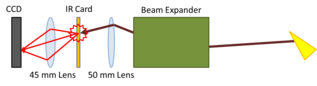
\includegraphics[width=10cm]{17_home_cooperw_RStudio_DEEPWAVE_WindUncertainty_BeamPointing_ReceiverDiagram-r.png} 
\par\end{centering}

\protect\protect\protect\protect\caption{\label{fig:TelescopePointingRX}Diagram of the receiver system. The
invisible infared beam enters the beam expander which amplifies the
angle of the beam relative to the telescope optic axis, and is then
focused onto an IR card. The IR card fluoresces at a visible wavelength
and that light is reimaged onto a CCD.}
\end{figure}


\begin{figure}
\noindent \begin{centering}
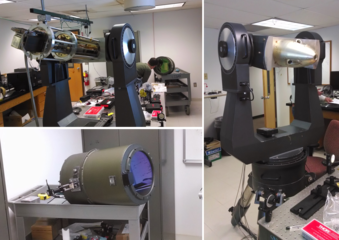
\includegraphics[width=10cm]{18_home_cooperw_RStudio_DEEPWAVE_WindUncertainty_BeamPointingCollection-r.png} 
\par\end{centering}

\protect\protect\protect\protect\caption{\label{fig:TelescopePictures}Photographs of the telescope angle measurement
system in the RAF optics lab. View of the setup from behind the LAMS
pod (top left), the receiver system (bottom left), LAMS mounted in
the telescope mount (right).}
\end{figure}


With the IR card at the back focus of the optical system, the beam
image is position independent. Its location in this plane is dictated
solely by the angle of the input beam. Even though each beam is slightly
translated relative to its counterparts, we can still perform accurate
angle measurements.

The LAMS system is mounted in a precision telescope mount with accuracy
on the order of $1^{\prime\prime}$ or about $0.0003^{\circ}$. The
mount gives fine resolution in adjusting LAMS pointing into the receiver
reference system and provides a digital readout of Alt/Az coordinates.
These coordinates provide the first set of pointing data for the LAMS
system. The second set of pointing data is provided by the SDN500
INS, which is attached and operating during our data collection. Thus,
two measurements of the LAMS pointing are provided.

The telescope mount readout provides the quantities Alt, $\vartheta_{T}$\sindex[lis]{theta\_T@$\vartheta_{T}$=altitude angle, telescope mount, LAMS calibration},
and Az, $\varphi_{T}$\sindex[lis]{phi\_T@$\varphi_{T}$=azimuth angle, telescope mount, LAMS calibration}.
When a beam is directed into the reference telescope, it is accomplished
through rotation operations: 
\begin{equation}
\hat{r}=\mathbf{R}(\vartheta_{T},\hat{x})\mathbf{R}(\varphi_{T},\hat{y})\hat{u},\label{TelMountReference}
\end{equation}
where $\hat{r}$ \sindex[lis]{r\_hat@$\hat{r}$=reference direction, LAMS receiving telescope, for
LAMS angle calibration}is the reference direction of the receiving telescope, $\hat{u}$
is the beam pointing direction and $\mathbf{R}(\theta,\hat{v})$\sindex[lis]{R\_LAMS@$\mathbf{R}(\theta,\hat{v})$=rotation matrix used for LAMS
calibration} is a rotation matrix of angle $\theta$ about the vector $\hat{v}$.

To determine the beam pointing angle, we invert the rotation operations
(or perform the opposite rotations in the opposite order), which results
in 
\begin{equation}
\hat{u}=\mathbf{R}(-\varphi_{T},\hat{y})\mathbf{R}(-\vartheta_{T},\hat{x})\hat{r}.\label{TelMountBeam}
\end{equation}
To obtain a beam pointing vector, we first need to know the reference
vector in some coordinate basis. We let Beam 4 (the forward pointing
beam) define the z-axis in this coordinate basis and obtain $\hat{r}$
by evaluating Eq. \eqref{TelMountReference} for the recorded Alt/Az
angles of Beam 4 (D) where $\hat{u}=\left[\begin{array}{ccc}
0 & 0 & 1\end{array}\right]^{T}$. We then obtain all other beam vectors from their respective Alt/Az
coordinates using Eq. \eqref{TelMountBeam}.

The process for obtaining the beam pointing vectors from the SDN500
IRU is essentially identical to the process above, except that the
SDN500 IRU provides roll, pitch and heading. It should be noted, as
will be addressed later, that the SDN500 IRU heading is not reliable
when the device is stationary.

After the pointing angles of the beams are obtained from the telescope
mount and SDN500 IRU, the pointing angles need to be compared. However,
the beam vectors are recorded in different coordinate frames and SDN500
IRU heading data cannot be treated as reliable. A transformation matrix
between these two frames and heading adjustments to SDN500 IRU are
determined using minimization of errors so we can compare the beam
pointing results. Table \ref{tab:AngleDiff} shows the difference
in angle between each of the four beams after optimizing the transformation
between the two coordinate frames. The two beam pointing measurements
give results that are quite close.

\begin{table}
\begin{minipage}[t]{0.93\columnwidth}%
\noindent \begin{center}
\begin{tabular}{>{\centering}p{2.5cm}>{\centering}p{7cm}}
\toprule 
\textbf{Beam}  &
\textbf{Angle difference between}\tabularnewline
SDN500 IRU and Telescope Mount &
\tabularnewline
\midrule
\midrule 
Beam 1 (A) &
\tabularnewline
(Upward)  &
$0.024^{\circ}$ \tabularnewline
\midrule 
Beam 2 (B) &
\tabularnewline
(Down-In)  &
$0.004^{\circ}$ \tabularnewline
\midrule 
Beam 3 (C) &
\tabularnewline
(Down-Out)  &
$0.003^{\circ}$ \tabularnewline
\midrule 
Beam 4 (D) &
\tabularnewline
(Forward)  &
$0.024^{\circ}$ \tabularnewline
\midrule 
\label{tab:AngleDiff}  &
\tabularnewline
\end{tabular}
\par\end{center}%
\end{minipage}
\end{table}


An assessment of the beam pointing accuracy was performed by translating
the focused beam across the IR card and finding the spread of angles
accepted by the optical system. The full angle field-of-view of the
system was approximately $2^{\prime}$ or about $0.02^{\circ}$. The
beam spot position can be repeated to greater accuracy than this (we
can see when it is well centered using the CCD), however this is probably
a reasonable uncertainty figure because the IR card may not be located
at the exact Fourier plane of the optical system. 

The benefits of the telescope beam measurement method\index{LAMS!angle calibration!telescope method}
are: 
\begin{itemize}
\item All four beams are measured without changes to the setup.
\item The measurement is \textquotedbl{}hands off\textquotedbl{}, so there
is very little risk of perturbing the system during the measurement
processes.
\item The process provides redundant angle measurements (SDN500 IRU and
the telescope mount).
\item The entire LAMS pod is used and referenced directly to the same SDN500
INS used in flight. 
\end{itemize}
The weaknesses of this method are: 
\begin{itemize}
\item Beam focal positions are not measured.
\item Setup and alignment of the system is time consuming (approximately
2 days).
\item The procedure still does not provide an absolute pointing measurement
because the telescope acceptance vector is not known. 
\end{itemize}
\begin{table}
{\footnotesize{}}%
\begin{minipage}[t]{0.93\columnwidth}%
\begin{tabular}{>{\centering}p{1.8cm}>{\centering}p{1.8cm}>{\centering}p{1.8cm}>{\centering}p{1.8cm}>{\centering}p{1.8cm}>{\centering}p{1.8cm}>{\centering}p{1.8cm}}
\toprule 
\textbf{Beam}  &
\textbf{$\theta_{L}$ Telescope}  &
\textbf{$\theta_{L}$ SDN500 IRU}  &
\textbf{$\theta_{L}$ Laser Survey}  &
\textbf{$\phi_{L}$ Telescope}  &
\textbf{$\phi_{L}$ SDN500 IRU}  &
\textbf{$\phi_{L}$ Laser Survey}\tabularnewline
\midrule
\midrule 
Beam 1 (A) &
 &
 &
 &
 &
 &
\tabularnewline
(Upward)  &
$35.03^{\circ}$  &
$35.08^{\circ}$  &
$34.95^{\circ}$  &
--\footnote{Beam 1 is used as the basis for $\phi=0$ in the relative pointing
coordinate frame}  &
--  &
-- \tabularnewline
\midrule 
Beam 2 (B) &
 &
 &
 &
 &
 &
\tabularnewline
(Down-In)  &
$34.86^{\circ}$  &
$34.85^{\circ}$  &
$34.96^{\circ}$  &
$119.74^{\circ}$  &
$119.74^{\circ}$  &
$120.01^{\circ}$\tabularnewline
\midrule 
Beam 3 (C) &
 &
 &
 &
 &
 &
\tabularnewline
(Down-Out)  &
$34.86^{\circ}$  &
$34.85^{\circ}$  &
$35.01^{\circ}$  &
$120.16^{\circ}$  &
$120.16^{\circ}$  &
$120.00^{\circ}$\tabularnewline
\midrule 
\label{tab:PointingAngles}  &
 &
 &
 &
 &
 &
\tabularnewline
\end{tabular}%
\end{minipage}{\footnotesize \par}
\end{table}


The following uncertainty analysis treats unknown biases in pointing
as random variables with standard deviations or variances. These figures
represent uncertainty, not stochastic processes. The resultant variances
provide bounds on the LAMS wind vector accuracy based strictly on
the instrument characterization, independent of other factors such
as signal fidelity.

The accuracy to which we know the LAMS relative beam pointing directly
impacts our estimates of airspeed and wind. A sequence of line-of-sight
velocity measurements is given by the equation: 
\begin{equation}
\vec{m}=\mathbf{U}\vec{v}_{L},\label{Vmeas}
\end{equation}
where $\vec{m}$ is the set of measurements (3 or 4 elements corresponding
to the number of beams in use), $\vec{v}_{L}$ is the air velocity
vector in the LAMS beam coordinate basis and $\mathbf{U}$ is the
matrix describing each beam's pointing angle given by 
\begin{equation}
\mathbf{U}=\left[\begin{array}{cccc}
\hat{u}_{1} & \hat{u}_{2} & \hat{u}_{3} & \hat{u}_{4}\end{array}\right]^{T},\label{Umatrix}
\end{equation}
where $\hat{u}_{i}$ is the $ith$ beam pointing direction. The exact
vector entries for $\mathbf{U}$ are dependent on which beams are
used for LAMS operation. For example, $\hat{u}_{4}$ would not be
included for HCR-TEST (post-DEEPWAVE configuration) where the down-inboard
beam was not used in that three beam configuration. For this analysis
the beam and air velocity vectors are defined in the LAMS relative
coordinate frame. Though this is not inherently required, it allows
the analysis presented in this section to flow directly into further
uncertainty analysis described in Section \ref{sub:Absolute}.

The covariance matrix of a beam pointing vector is given by 
\begin{equation}
\Sigma_{\hat{u}_{i}}^{2}=\left(\frac{\partial\hat{u}_{i}}{\partial\phi}\right)\sigma_{\phi}^{2}\left(\frac{\partial\hat{u}_{i}}{\partial\phi}\right)^{T}+\left(\frac{\partial\hat{u}_{i}}{\partial\theta}\right)\sigma_{\theta}^{2}\left(\frac{\partial\hat{u}_{i}}{\partial\theta}\right)^{T},\label{CovUvec}
\end{equation}
where $\sigma_{\phi}$ and $\sigma_{\theta}$ are the standard deviation
of the beam pointing angles. Note that the uncertainty in these angles
may be different for each beam, but this analysis will treat them
as identical.

The variance in a measurement due to beam pointing uncertainty is
given by 
\begin{equation}
\sigma_{m_{ii}}^{2}=\vec{v}_{L}^{T}\Sigma_{\hat{u}_{i}}^{2}\vec{v}_{L}.\label{measUncert}
\end{equation}
The uncertainty in the relative pointing angles are assumed to be
independent for each beam (common uncertainty in the instrument pointing
will be addressed in section \ref{sub:Absolute}). Thus the total
measurement covariance matrix is diagonal and given by 
\begin{equation}
\Sigma_{\vec{m}}^{2}=\left[\begin{array}{cccc}
\sigma_{m_{11}}^{2} & 0 & 0 & 0\\
0 & \sigma_{m_{22}}^{2} & 0 & 0\\
0 & 0 & \sigma_{m_{33}}^{2} & 0\\
0 & 0 & 0 & \sigma_{m_{44}^{2}}
\end{array}\right].\label{measCov}
\end{equation}


The total velocity uncertainty in the LAMS coordinate frame is ultimately
bounded by its covariance matrix 
\begin{equation}
\Sigma_{\vec{v}_{L}}^{2}=\mathbf{U}_{inv}\left(\Sigma_{\vec{m}}^{2}+\Sigma_{f}^{2}+\mathbf{U}\Sigma_{\vec{v}}^{2}\mathbf{U}^{T}\right)\mathbf{U}_{inv},\label{VlamsError}
\end{equation}
where the velocity uncertainty resulting from beam pointing uncertainty
is given by the covariance matrix $\Sigma_{\vec{m}}^{2}$ from Eq.
\eqref{measCov}, the uncertainty due to FFT Doppler peak estimation
is described by the covariance matrix $\Sigma_{f}^{2}$ and is defined
in section \ref{sub:FreqPrec}, the covariance matrix $\Sigma_{\vec{v}}^{2}$
is the result of velocity variability between the three or four beam
sample volumes with $\mathbf{U}$ being the beam projection matrix
from Eq. \eqref{Umatrix} and $\mathbf{U}_{inv}$ is the inversion
matrix for finding the total velocity vector from the three or four
line-of-sight measurements. In the case of the three beam LAMS, $\mathbf{U}_{inv}=\mathbf{U}^{-1}$.
However, because the four beam system is overdefined, a pseudo-inverse
may be used, or if the uncertainty in measurements are well known,
\begin{equation}
\mathbf{U}_{inv}=\left[\mathbf{U}^{T}\left(\Sigma_{L}^{2}\right)^{-1}\mathbf{U}\right]^{-1}\mathbf{U}^{T}\left(\Sigma_{L}^{2}\right)^{-1},\label{OptInv}
\end{equation}
where 
\begin{equation}
\Sigma_{L}^{2}=\Sigma_{\vec{m}}^{2}+\Sigma_{f}^{2}+\mathbf{U}\Sigma_{\vec{v}}^{2}\mathbf{U}^{T}.\label{TotalMeasUncert}
\end{equation}


Assuming the angle uncertainty of all four beams is approximately
$0.02^{\circ}$ and an aircraft velocity of 200 m/s along the LAMS
pointing direction, the total velocity uncertainty resulting from
beam pointing uncertainty is approximately 0.06 m/s in the horizontal
and vertical directions with the four beam configuration, 0.09 m/s
in the horizontal and vertical directions with the three beam configuration
used in HCR-TEST. To first order approximation, the forward velocity
is insensitive to small perturbations in beam pointing.

Add note that SDN500 IRU cannot provide reliable heading information
without moving. Heading adjustments had to be added to the fit of
the two measurements.


\subsubsection{SDN500 IRU Absolute Beam Pointing\label{sub:Absolute}}

With the relative pointing angles of the beams, an air velocity vector
can be retrieved reliably in the predefined LAMS coordinate frame.
However, the exact transformation between the LAMS beams and the SDN500
IRU coordinate frame (defined by the unit's principal axes) is unknown.
We typically assume that one SDN500 IRU axis is exactly aligned to
the forward pointing beam and one is directed along the angle beam
1. However, it stands to reason that there will be some slight differences
between the LAMS beam coordinate frame and the principal axes of the
SDN500 IRU. At present, the only method we have for determining this
transformation relies on making small angle adjustments based on flight
maneuvers.

Let the transformation matrix between the LAMS relative coordinate
frame and the SDN500 IRU principal axes be $\mathbf{T_{L}}$. The
velocity from LAMS is converted to the SDN500 IRU coordinate frame
using 
\begin{equation}
\vec{v}_{c}=\mathbf{T_{L}}\vec{v}_{L},\label{velL2C}
\end{equation}
where $\vec{v}_{c}$ is the air velocity vector in the SDN500 IRU
coordinate frame and $\vec{v}_{L}$ the air velocity vector in the
LAMS relative beam coordinate frame. To propagate error in the transformation
matrix we reframe the problem by vectorizing the matrix such that
Eq. \eqref{velL2C} becomes 
\begin{equation}
\vec{v}_{c}=\mathbf{V_{L}}\vec{t}_{L},\label{velL2Cvect}
\end{equation}
where the matrix $\mathbf{T_{L}}$ has been converted to the vector
$\vec{t}_{L}$ given by 
\begin{equation}
\vec{t}_{L}=\left[\begin{array}{cccc}
T_{11} & T_{12} & \cdots & T_{33}\end{array}\right]^{T},\label{T2vec}
\end{equation}
where $T_{ij}$ is the element of $\mathbf{T_{L}}$ from the $ith$
row and $jth$ column. The matrix $\mathbf{V_{L}}$ is constructed
from the LAMS coordinate frame velocity vector $\vec{v}_{L}$ and
is given by 
\begin{equation}
\mathbf{V_{L}}=\left[\begin{array}{ccccccccc}
v_{1} & v_{2} & v_{3} & 0 & 0 & 0 & 0 & 0 & 0\\
0 & 0 & 0 & v_{1} & v_{2} & v_{3} & 0 & 0 & 0\\
0 & 0 & 0 & 0 & 0 & 0 & v_{1} & v_{2} & v_{3}
\end{array}\right],\label{v2mat}
\end{equation}
where $v_{i}$ is the $ith$ element of $\vec{v}_{L}$.

The covariance matrix of $\vec{t}_{L}$ can be estimated from the
uncertainties in the roll, pitch and yaw transformation angles denoted
here as $\gamma$, $\beta$ and $\alpha$ respectively using partial
derivatives 
\begin{equation}
\Sigma_{\vec{t}_{L}}^{2}=\left(\frac{\partial\vec{t}_{L}}{\partial\gamma}\right)\sigma_{\gamma}^{2}\left(\frac{\partial\vec{t}_{L}}{\partial\gamma}\right)^{T}+\left(\frac{\partial\vec{t}_{L}}{\partial\beta}\right)\sigma_{\beta}^{2}\left(\frac{\partial\vec{t}_{L}}{\partial\beta}\right)^{T}+\left(\frac{\partial\vec{t}_{L}}{\partial\alpha}\right)\sigma_{\alpha}^{2}\left(\frac{\partial\vec{t}_{L}}{\partial\alpha}\right)^{T}.\label{tCov}
\end{equation}


Thus the velocity covariance matrix in the SDN500 IRU coordinate frame
is given by 
\begin{equation}
\Sigma_{\vec{v}_{c}}^{2}=\mathbf{V_{L}}\Sigma_{\vec{t}_{L}}^{2}\mathbf{V_{L}}^{T}+\mathbf{T_{L}}\Sigma_{\vec{v}_{L}}^{2}\mathbf{T_{L}}^{T},\label{CMvelError}
\end{equation}
where $\Sigma_{\vec{v}_{L}}$ is obtained from Eq. \eqref{VlamsError}.

It should be noted that a similar analysis can be performed for the
transformation between SDN500 IRU and a Global or aircraft coordinate
frame where uncertainties in SDN500 IRU roll, pitch and heading are
better known.

ADD DETAILS ON DETERMINING THIS TRANSFORMATION MATRIX FROM FLIGHT
DATA.

With the SDN500 IRU INS, the air velocity measurements can be transformed
into a global coordinate frame. The transformation matrix is determined
using $\mathbf{T_{1}}$, $\mathbf{T_{2}}$ and $\mathbf{T_{3}}$ from
the roll, pitch and yaw reported by SDN500 IRU. The analysis needed
for this step is covered in Section \ref{sub:EarthRef}.


\subsubsection{Frequency Precision\label{sub:FreqPrec}}

The LAMS A/D samples each beam detection channel at 200 MHz and performs
a 1024 point FFT. The frequency resolution of the FFT is thus given
by the sample rate divided by the number of data points 
\begin{equation}
\Delta f=\dfrac{f_{s}}{N_{s}}=195\mathrm{kHz}.
\end{equation}
The Doppler shift measured on a particular beam is 
\begin{equation}
f_{D}=\frac{2}{\lambda}\hat{u}\cdot\vec{v},\label{DopplerShift}
\end{equation}
where $\lambda$ is the laser wavelength (1560 nm), $\hat{u}$ is
the beam direction and $\vec{v}$ is the velocity vector of the air
relative to the instrument. A factor of two is included because the
Doppler shift is imposed twice, first when the beam is absorbed by
the aerosol and second when it is re-emitted. Along the beam line-of-sight,
each FFT bin corresponds to a velocity resolution of $\Delta v_{LOS}=0.15\mathrm{m/s}$.
%With post processing the backscatter Doppler peak can be determined at sub-bin resolution.  %This is accomplished using linear interpolation on the derivative of the backscatter peak to find the derivative zero crossing. However,
the peak in the detected Doppler spectrum can be determined with resolution
of about 0.3~bin by using a fit to the derivative of the spectrum.
%For the purposes of this analysis, we assume a sub-sample resolution of about 0.3, %giving This
gives a line-of-sight velocity resolution of about $\Delta v_{LOS}=0.05\mathrm{m/s}$.

The resulting covariance matrix for each line-of-sight velocity measurement
(only accounting for frequency accuracy) is diagonal with identically
distributed variances 
\begin{equation}
\Sigma_{f}^{2}=\left[\begin{array}{cccc}
\sigma_{v_{LOS}}^{2} & 0 & 0 & 0\\
0 & \sigma_{v_{LOS}}^{2} & 0 & 0\\
0 & 0 & \sigma_{v_{LOS}}^{2} & 0\\
0 & 0 & 0 & \sigma_{v_{LOS}}^{2}
\end{array}\right],\label{CovFreq}
\end{equation}
where, for our purposes, we assume $\sigma_{v_{LOS}}=\Delta v_{LOS}$.

The analysis presented here assumes variance in the sample rate to
be small compared to other error sources.

Note that at GV speeds, the Doppler shift is expected to exceed the
Nyquist frequency at the present sample rate. We use the true air
speed measurements from the aircraft radome to determine which frequency
fold contains the Doppler peak.


\subsubsection{Flow Distortion}

\index{LAMS!airflow distortion}Initial operation of the three beam
LAMS on IDEAS-4-GV revealed that the aircraft can influence flow fields
in the LAMS sample volume. This issue became recognizable when data
processing showed the down-inboard beam registered significantly slower
velocities than the other two beams. An analysis using Gulfstream's
computational fluid dynamics analysis confirmed that all three beams
could be expected to observe some flow distortion. The expected flow
distortion depends on the aircraft flight parameters. The down-inboard
beam is expected to experience the largest effect, typically observing
a line-of-sight flow effect between -0.5 and -2.0 m/s when the beam
is focused at 20 m. The upward beam may see flow effects on the order
of $\pm0.5$ m/s and the down-outboard may see flow effects between
0 and -0.5 m/s.

On the GV, LAMS no longer uses the down-inboard beam due to the substantial
flow effects in its sample volume. The flow effects around the C-130
will be better determined after the ARISTO flight campaign in Fall
2015.


\subsubsection{Uncertainty arising from separation of measurement volumes}

\index{LAMS!separation of measurement folumes}In turbulent conditions
the three sensitive volumes can be characterized by slightly different
values of the wind vector\sindex[lis]{v@$\mathbf{v}$=wind vector}
$\mathbf{v}=\{u,v,w\}.$ \sindex[lis]{u@$u$=component of wind along the x-axis}\sindex[lis]{v@$v$=component of wind along the y-axis}\sindex[lis]{w@$w$=component of wind along the z-axis}The
single forward beam measures $u$ directly while the 3-beam system
must solve for $u$ using the relative wind measurements at three
locations displaced from each other. If there are variations in the
wind vector at these three locations, that will introduce an error
that can be significantly larger than the measurement errors for a
single-beam-forward system.

If for simplicity it is assumed that the 3-beam system is aligned
so that the longitudinal axis matches the $u$ axis and the vertical
axis matches the $w$ axis, then the unique solution (for a 35$^{\circ}$
diverging-beam angle) for the true airspeed ($u$) is

\begin{equation}
u=\frac{(a_{1}+a_{2}+a_{3})}{3\cos(35^{\circ})}\label{eq:TAS3beam}
\end{equation}


where $a_{i}$ is the relative airspeed measured by the ith beam.%\footnote{The direction cosines for the three beams are given by the following matrix $\sigma$:% % \[% \sigma=\left(\begin{array}{ccc}% \cos\Theta & \sin\Theta\sin\Phi & \sin\Theta\cos\Phi\\% \cos\Theta & -\sin\Theta\sin\Phi & \sin\Theta\cos\Phi\\% \cos\Theta & 0 & \sin\Theta% \end{array}\right)% \]% where $\Theta=35^{\circ}$ and $\Phi=120^{\circ}$. The direction% cosine matrix relates the wind components to the 3-beam measured components% ($a_{i}$\} via % % \[% \begin{pmatrix}a_{1}\\% a_{2}\\% a_{3}% \end{pmatrix}=\mbox{\textbf{\ensuremath{\sigma}}}\begin{pmatrix}u\\% v\\% w% \end{pmatrix}% \]% % % Inverting $\sigma$ then gives the wind components in terms of the% measured components:% % \[% \begin{pmatrix}u\\% v\\% w% \end{pmatrix}=\sigma^{-1}\begin{pmatrix}a_{1}\\% a_{2}\\% a_{3}% \end{pmatrix}% \]% % % For the above angles, application of the inverse below to the component% $u$ leads to (\ref{eq:TAS3beam}): % % \[% \sigma^{-1}=\begin{pmatrix}0.4069249 & 0.4069249 & 0.4069249\\% 1.006579 & -1.006579 & 0\\% -0.5811489 & -0.5811489 & 0.9166754% \end{pmatrix}% \]% }If
each beam measures relative airspeed in its direction of alignment
to an uncertainty $\delta$,\sindex[lis]{delta@$\delta$=measurement uncertainty}
then a one-beam system aligned along the airflow measures with uncertainty
$\delta$ while a three-beam system measures to uncertainty $\sqrt{3}\delta/(3\cos(35^{\circ})=0.7\delta$,
so if each beam is an independent measurement the 3-beam system measures
TAS more accurately than a single-beam system. However, the unique
solution for the wind vector obtained from the 3-beam system relies
on the assumption that all three beams are viewing air that has the
same wind vector $\mathbf{v}$. If there is variation in the wind
vector at the three viewed locations, that variation is not necessarily
just variation in $u$ (that it might be desirable to average) but
can also result from other variations because the beams are not aligned
along the $u$ axis.

Because the uncertainty $\delta$ is less than 0.1 m/s, variations
of this magnitude would introduce errors comparable to the measurement
error. The spatial separation between any two sensitive volumes in
the 3-beam system is about 1.5($\sqrt{2}L\sin(35^{\circ})\simeq18$\,m
for focal distance L=15 m. The variance in the wind for points separated
by 18 m can be estimated as follows:\sindex[lis]{epsilon@$\epsilon$=eddy dissipation rate}\sindex[lis]{k@$k$=wave number}

\begin{equation}
(u^{\prime})^{2}=\int_{k_{0}}^{\infty}C\epsilon^{2/3}k^{-5/3}dk=\alpha\epsilon^{2/3}\frac{3}{2}k_{0}^{-2/3}\label{eq:Uvariance}
\end{equation}


where $k_{0}=2\pi/\Delta$ with $\Delta=18$ m. For modest eddy dissipation
rates in the range $\epsilon=0.001$ to 0.01 m$^{2}$s$^{-3}$, and
for $C=1.5$ (FIND REFERENCE XXX)\marginpar{XXX}, (\ref{eq:Uvariance})
results in estimates of the velocity variance of about .02--0.1 m$^{2}$s$^{-2}$,
or standard deviations of about 0.14 to 0.3 m/s. These fluctuations,
entering (\ref{eq:TAS3beam}), will cause errors in the estimate of
$u$ that are not negligible in comparison to the measurement errors
in \{$a_{1},\,a_{2},\,a_{3}$\}. {[}FIX THIS: C or $\alpha...$


\section{Calibration procedures\label{sec:CalProcedures}}


\subsection{Scope}

\index{calibrations!general}The measurements from the components
described in the preceding section are used to calculate the wind,
but those calculations also involve several empirically determined
relationships and adjustments arising either from calibrations or
flight maneuvers. This short section outlines the procedures used
for calibration and for determining those empirical relationships,
and it indicates where in this report the procedures are discussed
in more detail.


\subsection{Laboratory calibrations}

\index{calibrations!laboratory/bench}The key pressure sensors are
digital sensors having low uncertainty and good stability, so the
laboratory calibrations of those sensors are used primarily to ensure
performance within specifications rather than to make adjustments
to the output.

{[}{[}Dick and Jorgen: Could you provide a description of the pressure
calibration here?{]}{]}


\subsection{Quality-assurance checks}

\index{quality assurance!IRU}The output from the inertial sensors
is monitored primarily by comparison to other similar units. The duplicate
Honeywell inertial systems are compared on each flight to ensure that
their performance remains consistent, and when present the gust-pod
and LAMS inertial systems are also compared to each other and to the
Honeywell systems. The alignment angles of the various inertial systems
have been determined by survey and are not expected to change. Ground-speed
measurements from the inertial systems are compared routinely to GPS
measurements of ground speed, and the Schuler oscillations in ground-speed
components are monitored as indicators of the quality of these measurements.

Errors in the pitch measurement from the Honeywell inertial system
will result in errors in ground-speed components, so the differences
between inertial-system and GPS measurements of ground-speed components
can be used as indicators of the quality of the measurement of pitch.
This is discussed in detail in Sect.~\ref{sub:Schuler}, where a
procedure is also developed that can reduce the uncertainty in the
measurement of pitch.

\index{quality assurance!airflow angles}A calibration procedure for
determining angle of attack and sideslip angle is developed in Sect.~\ref{sec:Calibrations}.
To monitor the validity of the relationships determined there, the
equations employed (\eqref{eq:alphaWithwZero} and \eqref{eq:beta-equation})
are also used during projects for quality assurance to check that
the sensitivity coefficients in use give angle consistent with these
predictions.

\index{quality assurance!maneuvers}Some special maneuvers are used
frequently during projects to monitor the performance of the wind-measuring
systems. Pitch maneuvers,\index{maneuver!pitch} in which variations
in pitch lead to oscillating vertical motion of the aircraft, are
used to check that this motion does not enter the vertical-wind measurement
to any significant extent. (An example is discussed in Sect.~\ref{sub:Timing};
cf.~Fig.~\ref{fig:pitchManeuvers}.) Similar maneuvers with variations
in forced sideslip\index{maneuver!yaw} are checked to see that no
significant effects of the sideslip enter the final wind. Speed runs\index{maneuver!speed run}
provide good checks on the angle-of-attack relationships, and reverse-heading
maneuvers\index{maneuver!reverse heading} (where the aircraft flies
over the same drifting track in opposite directions) are also used
to check for offsets in measurements of airspeed and sideslip. Finally,
circle maneuvers\index{maneuver!circle} are used to check for errors
in airspeed, sideslip offset, or heading offset, as discussed below
(Sect.~\ref{sub:circle-summary}).


\subsection{Finding the relative-wind angles}

\index{angle!airflow}The angle of attack and sideslip angle are needed
to determine the relative wind\index{wind!relative} (cf.~\ref{sub:The-Relative-Wind}).
For the radome-based and gust-pod systems, these angles are not measured
directly but are determined from empirical relationships\index{relationships!empirical}\index{sensitivity coefficients|see {relationships, empirical}}
between the flow angles and pressure differences on the sensors. The
procedures for determining these empirical relationships are discussed
in Sect.~\ref{sec:Calibrations}.

In the case of angle of attack\index{attack!angle of}, the procedure
for determining the needed empirical relationship relies on assuming
that the vertical wind is negligible over the region covered by the
flight maneuver, which is normally a \textquotedbl{}speed run\textquotedbl{}\index{maneuver!speed run}
where flight speed is changed gradually over the flight envelope of
the aircraft. This assumption is checked by repeated calibrations,
but the absence of a standard for calibration leads to possible constant
bias in the vertical wind that remains a key source of uncertainty.
This is discussed in detail in Sect.~\ref{sub:radome-sensitivity}
for the radome system and Sect.~\ref{sub:gust-pod-aoa} for the gust-pod
system.

For sideslip,\index{sideslip} the calibration uses the heading as
a reference so the resulting empirical relationship relies on the
heading being accurate. The fit procedure is discussed in Sect.~\ref{sub:calibration-SS},
but an adjustment to that procedure is then determined from additional
flight maneuvers that permit separation of the offsets in sideslip
and heading. This is discussed in Sect.~\ref{sub:circle-summary}
below and in detail in Sect.~\ref{sub:Analysis-of-circle}.

The empirical relationships used to determine angle of attack and
sideslip angle are summarized in Sect.~\ref{sub:CalSummary}.


\subsection{True airspeed}

\index{airspeed}The measurement of true airspeed for the radome-based
system\index{system!standard} relies on the measurements of dynamic
and ambient or static pressure\index{pressure!ambient}\index{pressure!dynamic}
and so will be affected by any error in the static pressure. This
has been removed by calibration using the single-beam version of LAMS,\index{laser air-motion sensor}
as discussed in detail by \citet{CooperEtAl2014}. The procedure is
too involved to discuss in detail in this report, so that reference
should be consulted for the determination of uncertainty in true airspeed\index{airspeed!uncertainty}
from the conventional system on the GV. In that reference, an empirical
fit to the corrections determined by LAMS was found, and that fit
is now applied to all projects including those on which LAMS is not
present. The result is an uncertainty in true airspeed of about 0.1\,m/s
when the single-beam LAMS is available and about 0.3\,m/s otherwise.

The gust-pod system\index{system!gust pod}\index{gust pod} also
can be used to determine a measurement of true airspeed, but it requires
an involved fit to obtain good results. This measurement is useful
for two reasons. First if it may be desirable to obtain measurements
of wind from the gust pod without reference to the usual radome-based
system, for redundancy, backup, and quality control. Second, the gust
pod provides high-frequency measurements\index{turbulence!measurements}
that apparently are superior to those from the radome-based system.
Determining true airspeed from the gust pod is discussed in Sect.~\ref{sub:GP-TAS},
and there is a brief discussion of high-rate measurements and the
usefulness of the gust pod for such measurements in Appendix B.


\subsection{The circle maneuvers\label{sub:circle-summary}}

\index{maneuver!circle}\index{circle maneuver|see {maneuver, circle}}Flying
constant-roll-angle turns while drifting with the wind provides additional
opportunities for checks and adjustment of the empirical relationships\index{relationships!empirical}
and the airspeed measurement. The drift of the aircraft in such a
maneuver provides a good reference measurement of the wind that is
independent of all wind-sensing components on the aircraft except
the GPS. In addition, a plot of measured wind speed as a function
of the angle between the heading of the aircraft and the wind direction
is a very useful analysis tool because any error in true airspeed
will produce a difference from upwind to downwind flight while any
error in the combination of heading and sideslip angle will produce
a difference between the two portions of the circle that are crosswind.
Furthermore, the sideslip angle should have opposite sign in right-turn
circles vs.~left-turn circles, so this makes it possible to separate
a bias in the measurement of heading from a bias in the measurement
of sideslip angle.

The analysis of circle maneuvers is discussed in detail in Sect.~\ref{sub:Analysis-of-circle},
and there the offset in sideslip angle is adjusted. The circles provide
good evidence in support of the low uncertainty claimed for the true
airspeed measurement from the radome and for the quality of the measurements
of heading and sideslip angle.

%% LyX 2.1.2 created this file.  For more info, see http://www.lyx.org/.%% Do not edit unless you really know what you are doing.% \documentclass{article}% \usepackage{mathptmx}% \usepackage[T1]{fontenc}% \usepackage[latin9]{inputenc}% \usepackage{geometry}% \geometry{verbose}% \setcounter{secnumdepth}{2}% \setcounter{tocdepth}{2}% \setlength{\parskip}{\medskipamount}% \setlength{\parindent}{0pt}% \usepackage{booktabs}% \usepackage{amsmath}% \usepackage{amssymb}% \usepackage{graphicx}% \usepackage[unicode=true]%  {hyperref}% \usepackage{breakurl}% % \makeatletter% % %%%%%%%%%%%%%%%%%%%%%%%%%%%%%% LyX specific LaTeX commands.% %% Because html converters don't know tabularnewline% \providecommand{\tabularnewline}{\\}% % \AtBeginDocument{%   \def\labelitemii{\(\rightarrow\)}% }% % \makeatother% % \begin{document}


\section{Uncertainty components and summary\label{sec:Uncertainty-components}}


\subsection{General structure of an analysis of uncertainty}

\index{uncertainty!analysis!format}Here we follow a particular style
for construction of an analysis of uncertainty by including these
components:\index{}
\begin{enumerate}
\item {\uline{A description of the measuring system.}} Section 2 of
this report serves this function by providing extensive discussion
of each component contributing to the measurement of wind, and it
discusses what is known about specifications for uncertainty associated
with those components. It also includes description of the algorithm
leading to components of the measured wind, and it discusses the three
independent systems available for measuring wind on the GV. 
\item {\uline{Tests and calibrations.}} Sections \ref{sec:CalProcedures}
and \ref{sec:Calibrations} provide key information on how calibration
maneuvers are used to determine the sensitivity of some of the measurements
to components of the wind. Section\textasciitilde{}\ref{sec:Calibrations}
on calibration is key to the uncertainty analysis because to a large
extent many of the potential errors from sensors are removed by the
calibrations in this section, so the calibration becomes the central
factor affecting the final uncertainty. Other intermediate sections
discuss some specific tests applied to the measurements in order to
check or reduce the uncertainty limits associated with these measurements.
This report goes somewhat beyond a conventional analysis of uncertainty
in that there are new developments discussed here and some unconventional
ways of checking the measurements. 
\item {\uline{Discussion of the elemental contributions to uncertainty.}}
\index{uncertainty!elemental sources}This discussion will follow
in this section, but first it appears useful to provide a more general
although incomplete discussion of what is expected from that detailed
analysis. The standard tabulation of elemental sources of uncertainty
then follows in subsections \ref{sub:vw-elements} and \ref{sub:hw-elements}. 
\item {\uline{Summary and comprehensive estimate of uncertainty.}}
This follows at the end of this section and presents the key conclusions
of this study. 
\end{enumerate}
Because three wind-measuring systems are characterized in this report,
they will be discussed separately. However, the standard system is
the radome-based system, so that will be treated in the most depth.
The other two systems, the under-wing gust pod and the LAMS, are new
systems and their characteristics are still being developed and explored,
so their discussion necessarily will be incomplete until additional
flight data are collected.


\subsection{Preliminary estimates of uncertainty\label{subsub:prelim}}


\paragraph{Vertical wind.}

Because the calculation of wind from the contributing measurements
involves coordinate transformations, evaluation of the uncertainty
in wind components involves difficult error propagation through the
transformation matrices and other equations of Sect.~\ref{sub:General-comments}.
For application to straight-and-level flight (or flight where the
intent is to remain level), simplified equations suffice for evaluation
of the error terms. Evaluation of the more general case will not be
considered here and will likely benefit from Monte Carlo approaches.

For the vertical wind, Eq.~\ref{eq:Weq} provides an approximate
relationship that leads to straightforward error propagation, esp.~if
it is assumed that the angle of attack $\alpha$ and pitch $\theta$
are small angles so that\sindex[lis]{w\_p@$w_{p}$=upward velocity of the aircraft {[}m/s{]}}

\begin{equation}
w=V(\alpha-\theta)+w_{p}\label{eq:Weq-1}
\end{equation}
and errors in $w$ ($\delta w$) can be related to the errors in the
basic measurements ($\delta V$, $\delta\alpha$, $\delta\theta$,
$\delta w_{p}$) by differentiating Eq.~\ref{eq:Weq-1}: 
\begin{equation}
\delta w=(\alpha-\theta)\delta V+V(\delta\alpha-\delta\theta)+\delta w_{p}\,\,\,.\label{eq:delta-w}
\end{equation}
Correlations among these error terms are possible, so a full evaluation
that does not assume independence among the errors leads to:

\begin{eqnarray}
\left\langle (\delta w)^{2}\right\rangle  & = & (\alpha-\theta)^{2}\left\langle (\delta V)^{2}\right\rangle +V^{2}\left(\left\langle (\delta\alpha)^{2}\right\rangle +\left\langle (\delta\theta)^{2}\right\rangle \right)+\left\langle (\delta w_{p})^{2}\right\rangle \nonumber \\
 &  & +2\left((\alpha-\theta)\left(V(\left\langle \delta V\delta\alpha\right\rangle -\left\langle \delta V\delta\theta\right\rangle )+\left\langle \delta V\delta w_{p}\right\rangle \right)\right)\nonumber \\
 &  & +2V\left(\left\langle \delta\alpha\delta w_{p}\right\rangle +\left\langle \delta\theta\delta w_{p}\right\rangle \right)-2V^{2}\left\langle \delta\alpha\delta\theta\right\rangle \label{eq:delta-w-sq}
\end{eqnarray}


The approximate magnitudes of these terms, discussed in detail below,
are: $\delta V$=0.1~m/s, $\delta\alpha=0.1^{\circ}\simeq2$~mrad,
$\delta\theta\simeq1$~mrad, and $\delta w_{p}=0.03$~m/s. Other
typical magnitudes are $V\simeq200$~m/s, $\alpha\simeq\theta\simeq2^{\circ}\simeq3.5$~mrad.
For these typical magnitudes, the only terms in Eq.~\ref{eq:delta-w-sq}
that make potentially significant contributions are:

\begin{eqnarray}
\left\langle (\delta w)^{2}\right\rangle  & = & V^{2}\left(\left\langle (\delta\alpha)^{2}\right\rangle -2\left\langle \delta\alpha\delta\theta\right\rangle +\left\langle (\delta\theta)^{2}\right\rangle \right)\label{eq:delta-w-sq-simplified}
\end{eqnarray}


The error in pitch arises from measurements from the IRU and is affected
mostly by an initial offset during alignment and then further changes
in this error arising from the Schuler oscillation and from accelerations
that affect this error. The error in angle of attack, on the other
hand, arises from a combination of measurement error from the pressure
transducers and error in the formula used to deduce angle of attack
from the pressure measurements. This error is not independent of the
error in pitch, however, because the calibration as presented in Section
\ref{sub:Calibration-AOA} relies on the measured difference between
pitch and angle of attack being zero when the vertical wind and vertical
aircraft motion are zero. Thus any bias in pitch is transferred to
a bias in angle of attack, so this component of the error in \eqref{eq:delta-w-sq-simplified}
should cancel. The remaining errors arise from sources that are independent
and likely uncorrelated, so the middle term on the right side of \eqref{eq:delta-w-sq-simplified}
will be neglected in this preliminary analysis.

It is possible to estimate the magnitudes of these errors from measurements.
Because the GV instrumentation includes two identical inertial systems,
the difference in measurements of pitch from those two systems provides
one lower-bound estimate of the uncertainty in pitch. Measurements
discussed in Sect.~\ref{sub:Attitude-angles} suggest that, for periods
when the roll of the aircraft was within 5$^{\circ}$ of zero, the
difference between these redundant measurements was about 0.3~mrad
or less than about 0.02$^{\circ}$. Section \ref{sub:Schuler} presents
additional evidence from evaluation of the Schuler coupling between
pitch or roll errors and ground-speed errors, also indicating that
typical pitch errors are of about this magnitude. This is significantly
smaller than the manufacturer's specified uncertainty for this instrument,
$\pm0.05^{\circ}$.

This uncertainty in pitch is comparable to the estimated random uncertainty
in angle of attack, for which the variance spectra discussed in Sect.~\ref{sub:Variance-spectra-for-W-components}
suggest a random error of about 0.02$^{\circ}\simeq0.35$~mrad.\footnote{DEEPWAVE\textbf{\index{DEEPWAVE!flight 15}} flight 15, 3:40--3:55,
spectrum for AKRD, compared to simulated spectrum with random-noise
amplitude of 0.07. As generated, this has mean of half the amplitude,
so it corresponds to a standard deviation of .07/$\sqrt{12}\simeq0.02^{\circ}\simeq0.35$~mrad.} The estimated uncertainties in angle of attack and pitch are thus
comparable, and both influence the uncertainty in vertical wind.

The rough-estimate uncertainty in vertical wind (to be refined later)
is then, for flight at about 230~m/s, about $230\sqrt{0.0003^{2}+0.00035^{2}}\simeq0.1$~m/s.
Other factors, esp.~the radome calibration, need to be considered
for a refined estimate, as presented in Section \ref{sub:vw-elements},
but this is the general magnitude of uncertainty expected to result
from more refined analysis.\index{wind!uncertainty!preliminary estimate}


\paragraph{Horizontal wind}

Errors in measurements affect the longitudinal and lateral components
of the horizontal wind in different ways. For the longitudinal component
(along the aircraft longitudinal axis), the relative-wind measurement
(essentially the true airspeed) has been calibrated by comparison
to measurements of the single-beam LAMS, leading to an estimated standard
uncertainty of about 0.1~m/s (Cooper et al., 2014). The LAMS measurement
is based on measurement of the Doppler shift and thus has low limits
for bias and precision, dependent primarily on the uncertainty associated
with determining the peak in the returned Doppler spectrum in the
presence of turbulence. The lateral component is measured using the
sideslip angle, which is determined in a manner similar to that used
to calibrate the measurement of angle of attack. However, the zero
reference angle for attack is determined well by assuming that, on
average in quiescent air, the vertical wind should be zero. No similar
reference angle exists for sideslip, and trim adjustments to the aircraft
can change the mean sideslip angle, so a different procedure with
additional sources of uncertainty must be used.

Two maneuvers are particularly effective for determining the zero
reference for sideslip angle (at which angle the lateral horizontal
component of the relative wind would be zero): (i) Reverse-heading
maneuvers,\index{maneuver!reverse heading} where a straight leg is
flown for a short time (typically 2 min), then the aircraft reverses
heading and flies back along the reverse heading, with the result
that the wind component perpendicular to the longitudinal axis of
the aircraft should reverse sign; or (ii) constant-bank circles\index{maneuver!circle}
flown drifting with the wind, for which the lateral component of the
wind should exhibit a sinusoidal variation around the circle reflecting
a possible heading and/or sideslip error. Both maneuvers can provide
a reference for correcting a combination of heading and sideslip errors,
and the circle maneuver provides a mechanism for determining the sideslip
error alone, as discussed in Sect.~\ref{sub:Analysis-of-circle}.
There the uncertainty associated with the bias in sideslip was indicated
to be about 0.06$^{\circ}$ and the random uncertainty in heading
was estimated to be less than 0.09$^{\circ}$, with a bias limit comparable
to that in sideslip angle.

As for vertical wind, the GPS-measured components of aircraft motion
relative to the Earth have uncertainty\index{uncertainty!ground speed}
significantly less than that of the relative wind,\index{wind!relative}
so errors are dominated by those arising from the relative-wind components
and from the transformation to Earth coordinates.\index{coordinate system!Earth}
The first-order equation for the lateral component\sindex[lis]{vy@$v_{y}$=component of the horizontal wind lateral to the aircraft
axis} of the relative wind ($v_{y}$), analogous to Eq.~\ref{eq:Weq-1},
is $v_{y}=V\beta$ where $\beta$ is the sideslip angle. $V$ is known
to typically 0.05\% so the error is dominated by that in sideslip
angle and in heading. For the random error, one limit is obtained
as for angle of attack by examining the variance spectrum in calm
conditions. However, BDIFR and SSLIP\sindex[var]{SSLIP=sideslip variable selected for standard wind processing, usually
SSRD}\sindex[var]{SSRD=sideslip measurement from the standard radome-based system {[}deg{]}}
do not exhibit such pure noise spectra at high frequency as did ADIFR
and AKRD.\sindex[var]{AKRD=angle of attack from the standard radome-based system {[}deg{]}}\sindex[var]{ATTACK=angle of attack selected for standard wind processing, usually
AKRD} The QCF variance spectrum\index{variance spectrum!noise} has characteristics
of noise for amplitudes of random errors of about 0.15~hPa, slightly
higher than estimated for ADIFR. For BDIFR, an example is shown in
Fig.~\ref{fig:bdifrSpectrum}. 
\begin{figure}
\noindent \begin{centering}
\includegraphics[width=0.9\textwidth]{19_home_cooperw_RStudio_DEEPWAVE_WindUncertainty_BDIFRspectrum.png} 
\par\end{centering}

\protect\protect\protect\caption{\label{fig:bdifrSpectrum}Variance spectrum for BDIFR for DEEPWAVE\index{DEEPWAVE!flight 15}
flight 15, 3:40--3:55 UTC. The dashed orange lines indicate expected
white-noise spectra for respective standard deviations of 0.1 and
0.05~hPa. Units for $fP(f)$ are hPa$^{2}$ per logarithmic interval
in frequency.}
\end{figure}


The slope in the high-frequency region does not match that expected
for a white-noise signal, for which the variance would be constant
and in these plots, where the spectral density is multiplied by the
frequency, the plotted line should increase linearly with frequency
parallel to the orange dashed lines. Instead, the spectrum for BDIFR
has smaller slope than this, looking perhaps as if the spectrum starts
out at a point where a white-noise spectrum with standard deviation
0.1~hPa would be appropriate, but then is filtered or otherwise smoothed\footnote{perhaps by the response in the lines connecting the ports to the pressure
sensors} so that at the high-frequency limit the equivalent white-noise standard
deviation would be 0.05~hPa. The spectrum for SSLIP looks similarly
filtered, with an equivalent white-noise spectrum somewhere in the
range of 0.02$^{\circ}$, similar to that characterizing AKRD. However,
the estimated uncertainty in the bias for the combined effects of
sideslip angle and heading was, from the circle analysis, 0.02$\pm0.09^{\circ}$,
and these lead to contributions to the uncertainty in bias of the
lateral wind of about 0.3~m/s. The horizontal wind thus has an asymmetrical
estimated uncertainty, about three times as large for the lateral
component as for the longitudinal component.

Like vertical wind, this uncertainty estimate for the horizontal wind
needs to be refined for application to the Earth-relative wind by
consideration of the uncertainty in the determination of sensitivity
coefficients for sideslip angle and other contributions to the net
uncertainty in wind.


\subsection{Elemental sources, vertical wind\label{sub:vw-elements}}

Next, we tabulate the elemental sources of uncertainty\index{uncertainty!elemental sources!table}
in the measurement of vertical wind.\index{wind!vertical!uncertainty}


\subsubsection{Radome-based system}

Table~\ref{tab:Elemental-w} summarizes the results for the radome-based
wind system. The following is a discussion of the individual elements
in that table.

\begin{table}
\begin{tabular}{cccccc}
\toprule 
\textbf{element}  &
\textbf{uncertainty source}  &
\textbf{bias}  &
\textbf{random}  &
\textbf{$\delta w$ bias}  &
\textbf{$\delta w$ random }\tabularnewline
 &
 &
 &
 &
{[}m/s{]}  &
{[}m/s{]} \tabularnewline
\midrule
\midrule 
1  &
ADIFR transducer  &
0.07~hPa  &
0.002~hPa  &
--  &
--\tabularnewline
\midrule 
2  &
AKRD coefficients  &
0.01$^{\circ}$  &
0.001$^{\circ}$  &
0.04  &
0.004\tabularnewline
\midrule 
3  &
BDIFR transducer  &
0.07~hPa  &
0.002~hPa  &
--  &
--\tabularnewline
\midrule 
4  &
QCF transducer  &
0.34~hPa  &
0.01~hPa  &
<0.02  &
0.001\tabularnewline
\midrule 
5  &
pitch  &
0.02$^{\circ}$  &
0.007$^{\circ}$  &
0.08  &
0.03\tabularnewline
\midrule 
6  &
GV vertical velocity  &
0.03~m/s  &
<0.03~m/s  &
0.03  &
<0.03\tabularnewline
\midrule 
7  &
PSF transducer  &
0.10\,hPa  &
0.001\,hPa  &
--  &
--\tabularnewline
\midrule 
8  &
ATX  &
0.3$^{\circ}$  &
0.1$^{\circ}$C  &
--  &
--\tabularnewline
\bottomrule
\end{tabular}

\protect\protect\caption{Elemental contributions to the uncertainty in measurement of vertical
wind by the radome-based system. Entries '--' indicate negligible
contribution to uncertainty.\label{tab:Elemental-w}}
\end{table}

\begin{enumerate}
\item \textbf{ADIFR: }\index{angle!airflow}See Sect.~\ref{sub:Airflow-angles}
and Table~\ref{tab:Radome-system-measurements}. The uncertainty
is assigned to bias because it is likely a calibration uncertainty
and the resolution and stability are much smaller than this bias.
However, a calibration bias in this measurement does not affect the
final wind measurement because the procedure in Sect.~\ref{sub:radome-sensitivity}
determines the angle of attack from flight data in a way that can
be considered a calibration of the measurement of angle of attack,
and a bias in ADIFR would be reflected in a change in sensitivity
coefficients determined in that section that would compensate for
that bias. Only random errors in ADIFR would propagate to the final
measurement $w$, and such errors are thought to be negligible, so
the propagated error for ADIFR is listed as negligible. The next item
considers the determination of sensitivity coefficient for angle of
attack and is the dominant contribution to uncertainty in $w$ arising
from the measurement of angle of attack. 
\item \textbf{AKRD coefficients:} \index{relationship!empirical!angle of attack}The
calibration procedure of Sect.~\ref{sub:radome-sensitivity} effectively
removes the effects of possible biases in ADIFR and QCF and instead
replaces them with uncertainties arising from the coefficients \{$c_{0},\,c_{1}$\}
in (\ref{eq:AOArecommended}).\sindex[lis]{c0@$c_{0},\thinspace c_{1}$=coefficients leading to angle of attack
{[}deg.{]}} The estimated bias and random error are those obtained and discussed
in that section using the estimated uncertainties in the coefficients
in (\ref{eq:AOArecommended}). For propagation to vertical wind $w$,
(\ref{eq:VWind}) indicates that the result is approximately $\delta w=V\delta\alpha$
where $V$ is airspeed,\index{true airspeed|see airspeed} with additional
contributions from correlated errors involving $V$ that are small
in comparison to that listed. A typical value for V is about 240\,m\,s$^{-1}$,
leading to the listed elemental uncertainties in $w$ arising from
uncertainty in AKRD. It is important, though, that the calibration
is dependent on the assumption that the mean vertical wind where the
calibration data were collected be zero. This is discussed in Sect.~\ref{sub:radome-sensitivity}.
There is no independent way to check this except by comparing results
from different regions as done in this report. That remains a major
weakness in calibration and is the major contributor to uncertainty
in angle of attack, but it introduces a bias arising from a possible
calibration error. Fluctuations from the mean value are measured with
uncertainty a factor of ten smaller than this bias. The assumed mean
value of the vertical wind leading to this bias was $\pm$0.03\,m/s,
which could well be an over-estimate for the large datasets used in
Section~\ref{sub:radome-sensitivity}. 
\item \textbf{BDIFR:} \index{relationship!empirical!sideslip}The sideslip
angle has negligible effect on the vertical wind as long as the roll
angle is small, so for measurements made during straight-and-level
flight this contribution to uncertainty in vertical wind is negligible. 
\item \textbf{QCF:} \index{pressure!dynamic!uncertainty}The values listed
are the characteristics of the transducer. Application of the calibration
procedure based on comparison to the \index{laser air-motion sensor}laser
air-motion sensor (\citet{CooperEtAl2014}) led to an alternate uncertainty
estimate of 0.3\,hPa. As in the case of ADIFR, the procedure to determine
sensitivity coefficients removes any effect of bias in QCF by calibration
in terms of the coefficients \{$c_{0},\,c_{1}$\} so the effect on
bias in $w$ is replaced by possible bias in those coefficients, as
discussed for element 2. The effect of a random error in QCF of 0.01~hPa
is, from (\ref{eq:AOArecommended}). to introduce an uncertainty in
angle of attack of about 0.0002$^{\circ}$ or a contribution to uncertainty
in $w$ of less than 0.001\,m\,s$^{-1}$. QCF is also used to determine
the true airspeed, which affects $w$, but the effect is negligible
for the estimated uncertainty in QCF (<0.2\% of the measured value
of $w$, or 0.02\,m\,s$^{-1}$ for 10\,m\,s$^{-1}$ vertical wind). 
\item \textbf{PITCH:} \index{pitch!uncertainty}The estimates listed are
those that apply without the pitch-correction procedure of Sect.~\ref{sub:Schuler}.
In that section, it was estimated that the standard error in pitch
is 0.02$^{\circ}$ and that this is primarily in the form of a slowly
varying error that, over measurement periods short compared to the
Schuler oscillation period of 84.4~min, will appear as a bias. The
correction procedure represented by Eq.~\ref{eq:pitch-error-wo-approx}
corrects for this error well enough to leave the residual bias negligible,
so the bias entry in Table~\ref{tab:Elemental-w} can be eliminated
by application of that algorithm. The partitioning between bias and
random uncertainty depends on the interval considered, because Schuler
precession will cause variation in this error with the Schuler-oscillation
period of about 84 min. For periods long compared to this the error
will have the character of a random-error component, so using 0.08\,m/s
would be appropriate for random uncertainty of such long-term measurements
while the bias should be reduced substantially, perhaps to 0.02\,m/s.
For periods small compared to the Schuler period, the pitch error
appears as a bias and there is a much smaller random error, evaluated
in Sect.~\ref{sub:Attitude-angles} to be about 0.007$^{\circ}$
in pitch or about 0.03\,m/s in vertical wind. This is the usual case
for measurements of interest, so the bias and random errors are partitioned
as appropriate for this case in the table. The uncertainty in pitch
is the leading contributor to the standard uncertainty in vertical
wind and is also the leading contributor to the overall estimate of
bias. The correction technique of Sect.~\ref{sub:Schuler} is not
incorporated in routine processing so needs special calculation. 
\item \textbf{Aircraft Vertical Velocity:} \index{speed!vertical!aircraft}The
measurement used for vertical motion of the aircraft is discussed
is Sect.~\ref{sec:VerticalVelocity}. The values listed here are
those specified for measurements when ``OmniSTAR'' corrections\index{OmniSTAR}
are available; if not, the values should be increased to about 0.1\,m\,s$^{-1}$
and so will make a contributor to uncertainty in vertical wind that
is comparable to the contributions from pitch and angle of attack.
The error in aircraft vertical speed is likely a mixture of bias and
random error, because the primary source is uncertainty in ionospheric
corrections which will be persistent for important parts of flights
but likely to change at least from flight to flight. Because of the
likely persistence of the error, it is assigned here primarily to
bias. 
\item \textbf{PSF:} \index{pressure!ambient!uncertainty}The measured ambient
pressure affects vertical wind only through the dependence of true
airspeed T on PSF, as described in the document on \href{https://drive.google.com/file/d/0B1kIUH45ca5ATFV5d3QyQ0JpSjA/view?usp=sharing}{RAF processing algorithms},
Section 4.7.1. Evaluation at typical values shows that the dependence
of measured vertical wind on uncertainty in this variable is negligible.
For example, the airspeed for PSF=300\,hPa,\sindex[var]{PSF=ambient or static pressure measured at the fuselage static buttons
{[}hPa{]}} QCF=80\,hPa, and ATX=$-40^{\circ}$C differs from that for PSF=300.1
by 0.03\,m\,s$^{-1}$ or about 0.01\%, so this would also be the
percentage change in vertical wind. 
\item \textbf{ATX:} Temperature is needed to calculate the true airspeed,
but as for ambient pressure the effect of uncertainty in temperature
is very small. This was tested as for PSF by evaluating at representative
points. A representative result was that the listed bias in temperature
would lead to a bias in airspeed of about 0.05\%, leading to a similar
percentage change in the value of the vertical wind. This is negligible
in comparison to other sources of uncertainty. 
\end{enumerate}
The result of adding the elemental sources of uncertainty\index{uncertainty!vertical wind}\index{wind!vertical!net uncertainty}
in quadrature is a bias estimate of 0.10\,m\,s$^{-1}$ and a random-uncertainty
estimate of 0.04\,m\,s$^{-1}$, with pitch correction.\index{pitch!correction to}
Without the correction, the bias estimate increases to 0.35\,m\,s$^{-1}$,
so the pitch correction results in significant reduction in uncertainty
and without that correction the uncertainty is dominated by the bias
introduced by the measurement of pitch. In the corrected case, the
dominant contributions are those from pitch and angle of attack, as
was argued in the preliminary discussion in Section~\ref{subsub:prelim}.
The bias and random errors from pitch and from angle of attack, as
listed here, arise from different sources so it is reasonable to combine
them in quadrature to obtain composite estimates.

The APPLANIX\index{IRU!APPLANIX} IRU should provide another route
to improvement in the measurement of pitch, because it offers significantly
lower specified uncertainty. It achieves this through use of a full
Kalman-filter\index{filter!Kalman} correction to the measurements,
which would remove the need for the pitch correction\index{pitch!correction}
proposed in this document.


\subsubsection{Gust-pod system}

For the gust pod\index{gust pod}\index{system!gust pod} system,
many of the uncertainties associated with measurement components are
known less well than for the radome system, but some similar estimates
can be made. This section will duplicate the structure of the radome-based
system, but will be less definitive and more sketchy in some of the
components while emphasizing the differences that apply to the gust
pod.

Table~\ref{tab:GP-Elemental-w} lists the elemental contributions
to uncertainty\index{uncertainty!elemental sources!table}\index{wind!vertical!uncertainty}
in the measurement of vertical wind from the gust-pod system. The
following is a discussion of the individual elements in that table.\sindex[var]{AK_GP=angle of attack determined using the gust pod [deg]@AK\_GP=angle of attack determined using the gust pod {[}deg{]}}

\begin{table}
\begin{tabular}{cccccc}
\toprule 
\textbf{element}  &
\textbf{uncertainty source}  &
\textbf{bias}  &
\textbf{random}  &
\textbf{$\delta w$ bias}  &
\textbf{$\delta w$ random }\tabularnewline
 &
 &
 &
 &
{[}m/s{]}  &
{[}m/s{]} \tabularnewline
\midrule
\midrule 
1  &
ADIF\_GP transducer  &
0.07~hPa  &
0.002~hPa  &
--  &
--\tabularnewline
\midrule 
2  &
AK\_GP coefficients  &
0.01$^{\circ}$  &
0.001$^{\circ}$  &
0.04  &
0.004\tabularnewline
\midrule 
3  &
BDIF\_GP transducer  &
0.07~hPa  &
0.002~hPa  &
--  &
--\tabularnewline
\midrule 
4  &
QCF/QC\_GP transducer  &
0.34~hPa  &
0.01~hPa  &
0.02  &
0.001\tabularnewline
\midrule 
5  &
pitch  &
0.04$^{\circ}$  &
0.02$^{\circ}$  &
0.17  &
0.08\tabularnewline
\midrule 
6  &
GV vertical velocity  &
--  &
0.07~m/s  &
--  &
0.07\tabularnewline
\midrule 
7  &
PS\_GP transducer  &
0.10\,hPa  &
0.001\,hPa  &
--  &
--\tabularnewline
\midrule 
8  &
ATX  &
0.3$^{\circ}$  &
0.1$^{\circ}$C  &
--  &
--\tabularnewline
\bottomrule
\end{tabular}

\protect\protect\caption{Elemental contributions to the uncertainty in measurement of vertical
wind using the gust pod. Entries '--' indicate negligible contribution
to uncertainty.\label{tab:GP-Elemental-w}}
\end{table}

\begin{enumerate}
\item \textbf{ADIF\_GP: }See Sect.~\ref{sub:Airflow-angles} and Table~\ref{tab:Radome-system-measurements}
and the discussion related to the radome. The same transducers are
used for the pressure measurements on the gust pod, although the configuration
of ports is different. The next item considers the determination of
sensitivity coefficient for angle of attack and is the dominant contribution
to uncertainty in $w$ arising from the measurement of angle of attack. 
\item \textbf{AK\_GP coefficients:} The calibration procedure of Sect.~\ref{sub:gust-pod-aoa}
effectively removes the effects of possible biases in ADIFR and QCF
and instead replaces them with uncertainties arising from the fit
coefficients \{$b_{0--3}$\} in (\ref{eq:AOAGfunction}).\sindex[lis]{b0@$b_{0},\thinspace b_{1},\thinspace b_{2}\thinspace,b_{3}$=empirical
coefficients relating angle of attack to pressure measurements from
the gust pod {[}deg{]}} It was necessary to use additional terms to obtain a good fit in
this case, but the final result provided a very good representation
of the data, as good as in the radome case. We have therefore used
the same uncertainty estimate as for the radome, although with less
justification and study. As for the radome, the dominant source of
bias is again the uncertainty in vertical wind in the calibration
region, which is the same for this data set as for that used to determine
the radome sensitivity coefficients, so this estimate remains the
same as for the radome. The uncertainties also propagate to the vertical
wind in the same way. However, the restriction to low roll angle (less
than 5$^{\circ}$ from vertical) is still more important in the case
of the gust pod because the CMIGITS IRU used with the gust pod is
not aligned with the aircraft longitudinal axis but rather is mounted
in an under-wing pod that was designed to point into the airflow and
therefore slightly inward relative to the longitudinal axis. That
causes significant problems in turns because the IRU rotates in ways
that mix the attitude angles.
\item \textbf{BDIF\_GP:} The sideslip\index{sideslip} angle has negligible
effect on the vertical wind as long as the roll\index{roll} angle
is small, so for measurements made during straight-and-level flight
this contribution to uncertainty in vertical wind is negligible. 
\item \textbf{QCF and QC\_GP:} \index{pressure!dynamic!uncertainty}Two
measurements are listed because both are used in the calculation of
vertical wind. QC\_GP is used with ADIF\_GP to determine the angle
of attack, and the calibration described with item 2 effectively replaces
uncertainty in this measurement with uncertainty in the sensitivity
coefficients. However, true airspeed is determined using QCF because
the conventional true airspeed is thought to be superior to the new
value determined solely from the gust pod (Section~\ref{sub:GP-TAS}).
Therefore, the effect of uncertainty in QCF on vertical wind is the
same as that for the radome because the same calculated true airspeed
is used for both. 
\item \textbf{pitch (CPITCH\_GP):} \sindex[var]{CPITCH_GP@CPITCH\_GP}As
was the case for the cabin-mounted inertial systems, there were two
nearly identical inertial systems used in the wing pods, one for the
gust pod\index{gust pod} and the other for the LAMS,\index{laser air-motion sensor}
so it is again possible to compare the measurements and obtain estimates
of the random errors in their measurements. For both units (LAMS and
gust pod), the inertial systems use GPS measurements with a Kalman
filter\index{filter!Kalman} to apply corrections, but they align
independently and so have different errors and Schuler\index{Schuler oscillation|see {oscillation, Schuler}}
oscillations. There were many flights in DEEPWAVE\index{DEEPWAVE!missing data}
where one of these was not operational: 1--4, 6--7, 15, 17, 19. For
the other flights, the standard deviation in the difference in pitch\index{pitch!intercomparison}
between these two units was 0.06$^{\circ}$, so this is a reasonable
estimate of the random error that characterizes these measurements.\footnote{The standard deviation in the difference between two variables is
actually $sqrt(2)\times\delta$ where $\delta$ is the standard deviation
in each variable, so a better estimate is 0.04; this correction has
not been made throughout this document.}As for the radome, a true bias in this measurement (e.g., from misalignment
at installation) has been subsumed by the calibration of item 2 so
does not enter in this item. However, the remaining error on most
flights has a slowly varying component (consistent with the long time
period of the Schuler oscillation) and so appears as a bias for any
measurement made over a period short compared to the Schuler oscillation,
so it appears appropriate to assign the observed standard deviation
primarily to a bias because it will appear steady in normal applications
that look at vertical wind over periods short compared to the Schuler
oscillation. We have therefore partitioned the standard deviation
into estimated components of 0.04$^{\circ}$ bias and $0.02^{\circ}$
random error. The uncertainty in pitch is the leading contributor
to the standard uncertainty in vertical wind and is also the leading
contributor to the overall estimate of bias.
\item \textbf{Aircraft Vertical Velocity:} \index{speed of aircraft!vertical}For
the gust pod, the measurement of vertical motion of the aircraft must
be that from the IRU mounted in the under-wing pod because the wing
can flex and vibrate and the aircraft can roll in ways that cause
that vertical motion to differ from that sensed in the cabin. Again,
comparing the two units mounted in side-by-side wing pods provides
the best indication of the random component of uncertainty in this
measurement, because both units experience almost identical vertical
motion. These two units measure project-mean vertical aircraft motions
that differ by 0.04\,m/s, with standard deviation in that difference
of 0.07\,m/s. It seems reasonable then to estimate the random component
of uncertainty as 0.07\,m/s, but the bias is more uncertain. Good
flights usually produced mean vertical aircraft motion from takeoff
to landing of less than 0.005\,m/s, so it is reasonable to neglect
the possible bias in this measurement (which is updated for stability
in the IRU using pressure altitude as a reference).
\item \textbf{PSF:} \index{pressure!ambient!uncertainty}The measured ambient
pressure affects vertical wind only through the dependence of true
airspeed  on PSF, as described in the document on \href{https://drive.google.com/file/d/0B1kIUH45ca5ATFV5d3QyQ0JpSjA/view?usp=sharing}{RAF processing algorithms},
Section 4.7.1. The effect is the same as for the radome, and is negligible;
see the discussion above for the radome system. 
\item \textbf{ATX:} Temperature\index{temperature!uncertainty}\index{uncertainty!temperature}
is needed to calculate airspeed, but as for ambient pressure the effect
is negligible. See the radome discussion above. 
\end{enumerate}
The result of adding the elemental sources of uncertainty\index{uncertainty!wind!vertical}\index{wind!vertical!net uncertainty}
in quadrature is a bias estimate of 0.18\,m\,s and a estimate of
random uncertainty of 0.11\,m\,s$^{-1}$. The dominant contribution
in both cases is that from measured pitch, although the uncertainty
in vertical motion of the aircraft also makes a significant contribution
to the random component of uncertainty. \index{gust pod!limitations}It
is important that these estimates only apply to cases where the roll
is within 5$^{\circ}$ of level.


\subsection{Elemental sources, horizontal wind\label{sub:hw-elements}}


\subsubsection{Radome-based system}

Table \ref{tab:Elemental-h} lists the elemental contributions to
uncertainty\index{uncertainty!elemental sources} in the measurement
of horizontal\index{wind!horizontal!uncertainty} wind\index{wind!horizontal}
from the radome-based system. The following itemization discusses
each element.

\global\long\def\myparallel{{\mkern3mu\vphantom{\perp}\vrule depth 0pt\mkern2mu\vrule depth 0pt\mkern3mu}}
 
\begin{table}
\begin{tabular}{cccccc}
\toprule 
\textbf{element}  &
\textbf{uncertainty source}  &
\textbf{bias}  &
\textbf{random}  &
$\delta u_{\perp,\,\myparallel}$ \textbf{bias}  &
$\delta u_{\perp,\,\myparallel}$ \textbf{random }\tabularnewline
 &
 &
 &
 &
{[}m/s{]}  &
{[}m/s{]} \tabularnewline
\midrule
\midrule 
1  &
BDIFR transducer  &
0.07~hPa  &
0.002~hPa  &
--  &
--\tabularnewline
\midrule 
2  &
SSRD coefficients  &
0.03$^{\circ}$  &
0.002$^{\circ}$  &
(0.12,~--)  &
(0.01,~--)\tabularnewline
\midrule 
3  &
ADIFR transducer  &
0.07~hPa  &
0.002~hPa  &
--  &
--\tabularnewline
\midrule 
4  &
QCF transducer  &
0.34~hPa  &
0.01~hPa  &
(see item 9)  &
\tabularnewline
\midrule 
5  &
heading  &
0.09$^{\circ}$  &
0.04$^{\circ}$  &
(~0.38, --)  &
(0.17,~--)\tabularnewline
\midrule 
6  &
pitch  &
0.02$^{\circ}$  &
0.02$^{\circ}$  &
--  &
--\tabularnewline
\midrule 
7  &
horiz. velocity of GV  &
0.03~m/s  &
<0.03~m/s  &
0.03  &
0.03\tabularnewline
\midrule 
8  &
PSF transducer  &
0.10\,hPa  &
0.001\,hPa  &
--  &
--\tabularnewline
\midrule 
9  &
ATX  &
0.3$^{\circ}$  &
0.1$^{\circ}$C  &
(--,~0.16)  &
(--,~0.05)\tabularnewline
\midrule 
10  &
$\delta q$  &
0.2\,hPa  &
0.1\,hPa  &
(--,~0.3)  &
(--,~0.15)\tabularnewline
\bottomrule
\end{tabular}

\protect\protect\caption{Elemental contributions to the uncertainty in measurement of horizontal
wind by the radome-based system. Entries '--' indicate negligible
contribution to uncertainty. Entries with subscript $\perp$ refer
to the lateral component of the horizontal wind, and those with subscript
indicating parallel refer to the longitudinal component (along the
axis of the aircraft). \label{tab:Elemental-h}}
\end{table}

\begin{enumerate}
\item \textbf{BDIFR:} \sindex[var]{BDIFR}The primary uncertainty in BDIFR
is assigned to bias because it is likely a calibration uncertainty
and the resolution and stability are much smaller than this bias.
However, a calibration bias in this measurement does not affect the
final wind measurement because the procedure in Sect.~\ref{sub:radome-sensitivity}
determines the sideslip angle from flight data in a way that can be
considered a calibration of the measurement of sideslip angle, and
a bias in BDIFR would be reflected in a change in sensitivity coefficients
determined in that section that would compensate for that bias. Only
random errors in BDIFR propagate to the final measurement of horizontal
wind, and the effect of the listed random error is typically less
than 0.0001 m/s in lateral wind, with even smaller contribution to
the longitudinal wind. These contributions therefore are listed as
negligible in the table. The next item considers the determination
of sensitivity coefficient for sideslip angle and is the dominant
contribution to uncertainty in horizontal wind arising from the measurement
of sideslip angle. 
\item \textbf{SSRD coefficients:} \sindex[var]{SSRD}The calibration procedure
of Sect.~\ref{sub:radome-sensitivity} effectively removes the effects
of possible biases in BDIFR and QCF and instead replaces them with
uncertainties arising from the \sindex[lis]{e0@$e_{0},\thinspace e_{1}$=empirical coefficients used to obtain
the sideslip angle}coefficients \{$e_{0},\,e_{1}$\} in (\ref{eq:betaFunctionForm})
and the ability of the selected formula to represent the calibration
data. The uncertainty in the first coefficient, the main contributor
to sideslip bias, is obtained from the standard deviation in the mean
of results from the circle analysis, summarized in Sect.~\ref{sub:HWsummary}.
For propagation to lateral horizontal wind, (\ref{eq:horizWindeqs})
indicates that the result is approximately $\delta u_{lateral}=V\delta\beta$
where $V$ is airspeed, with additional contributions from correlated
errors involving $V$ that are small in comparison to that listed.
A typical value for V is about 220\,m\,s$^{-1}$, leading to the
listed elemental uncertainties in horizontal wind arising from uncertainty
in SSRD. 
\item \textbf{ADIFR: }\sindex[var]{ADIFR}See Sect.~\ref{sub:Airflow-angles}
and Table~\ref{tab:Radome-system-measurements}. The angle of attack
has negligible effect on the horizontal wind as long as the roll angle
is small, so for measurements made during straight-and-level flight
this contribution to uncertainty in horizontal wind is negligible. 
\item \textbf{QCF:} \sindex[var]{QCF}\index{pressure!dynamic!uncertainty}The
values listed are the characteristics of the transducer. Application
of the calibration procedure based on comparison to the laser air-motion
sensor (\citet{CooperEtAl2014}) led to an estimated standard uncertainty
of 0.1~m/s for steady flight conditions and 0.3~m/s for fluctuating
conditions, so this is used for the table entry pertaining to the
wind component in the direction of the longitudinal axis of the aircraft.
For the lateral component, QCF affects the calculated sideslip angle
SSRD, but as in the case of AKRD the procedure to determine sensitivity
coefficients removes any effect of bias in QCF by calibration in terms
of the coefficients \{$c_{0},\,c_{1}$\} so a potential bias in QCF
does not enter the lateral component of the horizontal wind but instead
is replaced by possible bias in those coefficients, as discussed for
element 2. The effect of a random error in QCF of 0.01~hPa for a
typical value of QCF$\approx$100\,hPa is, from (\ref{eq:betaFunctionForm}),
to introduce an uncertainty in sideslip angle of about 0.01\% or,
because typical values of sideslip angle are smaller in magnitude
than 1$^{\circ}$, an error propagated to horizontal wind smaller
than 0.001~m/s. This contribution is therefore neglected. 
\item \textbf{HEADING:} \sindex[var]{THDG}\index{heading!uncertainty}\index{uncertainty!heading}The
random error in heading can be evaluated by comparing two duplicate
IRUs, as was done for pitch. The two systems on the GV for DEEPWAVE
differed in mean heading by about 0.45$^{\circ}$, evidently a result
of an alignment error on installation. However, the standard deviation
of the difference between the two measurements was only 0.04$^{\circ}$,
a value that indicates the systems may perform better than the manufacturer's
specification (0.2$^{\circ}$) would indicate. The uncertainty in
the bias evaluated from the circle-maneuver study of Sect.~XXX is
about 0.09$^{\circ}$, so this will be used as the bias estimate while
0.04$^{\circ}$ is considered the random component of uncertainty
in heading. 
\item \textbf{PITCH:} \sindex[var]{PITCH}\index{pitch!uncertainty}The
contribution to uncertainty from the measurement of pitch was discussed
above in connection with measurement of the vertical wind. However,
in the case of horizontal wind, for level flight with negligible roll
an uncertainty in pitch makes negligible contribution to uncertainty
in either component of the horizontal wind. 
\item \textbf{Horizontal Velocity Components of the Aircraft:} \index{speed of aircraft!ground speed!uncertainty}The
measurement of horizontal wind is the sum of the relative wind\index{wind!relative}
and the horizontal motion of the aircraft relative to the Earth, so
uncertainty in this component enters directly into uncertainty in
the measured wind components. 
\item \textbf{PSF:} \sindex[var]{PSF}\index{pressure!ambient!imcertainty}The
measured ambient pressure affects horizontal wind only through the
dependence of true airspeed on ambient pressure, as described in the
document on \href{https://drive.google.com/file/d/0B1kIUH45ca5ATFV5d3QyQ0JpSjA/view?usp=sharing}{RAF processing algorithms},
Section 4.7.1. Evaluation at typical values shows that the dependence
of the measured lateral component of the horizontal wind on uncertainty
in this variable is negligible. For example, TASF for PSF=300\,hPa,
QCF=80\,hPa, and ATX=$-40^{\circ}$C differs from that for PSF=300.1
by 0.03\,m\,s$^{-1}$ or about 0.01\%, so this would also be the
percentage change in the lateral component of the relative wind. 
\item \textbf{ATX:} \sindex[var]{ATX}\index{temperature!uncertainty}\index{uncertainty!temperature}Temperature
is needed to calculate airspeed. Other studies (\citet{CooperEtAl2014})
indicate that the temperature uncertainty is about 0.3$^{\circ}$C,
and this error will propagate to uncertainty in both components of
the horizontal wind. Typical values of Mach\index{Mach number} number
for the DEEPWAVE\index{DEEPWAVE!typical Mach number} project were
0.8, for which a temperature change of $+0.3^{\circ}$C led to an
increase in true airspeed of about 0.16\,m/s. The temperature error
is likely a bias, so this difference also should be treated as a bias.
The result is that the longitudinal component of the horizontal wind
has an elemental contribution from temperature of 0.16\,m/s, while
the lateral component (being small and having an error proportional
to the error in airspeed of about 0.16/240 or smaller than 0.1\%)
has negligible error from this source. 
\item \textbf{PCOR:} \index{pressure!correction}\index{PCOR|see {pressure, correction}}\sindex[var]{PCOR=correction applied to measured ambient and dynamic pressures}The
dynamic and static pressure\index{pressure!dynamic}\index{pressure!static}
measurements are corrected for the static defect at the pressure ports
using the formulas developed in (\citet{CooperEtAl2014}). The uncertainty
in the determination of the correction was estimated in that source
as less than 0.3\,m/s. Here we use similar estimates of 0.2 (bias)
and 0.1\,hPa (random error). correlated such that the error in static
pressure is the negative of the error in dynamic pressure. For DEEPWAVE\index{DEEPWAVE}
research flights these errors propagate to 0.3\,m/s bias and 0.15\,m/s
random uncertainty. 
\end{enumerate}
For the lateral\index{wind!uncertainty!lateral}\index{uncertainty!wind!lateral}\index{wind!lateral component}
component of the wind, adding the elemental contributions to uncertainty
in quadrature leads to a net bias estimate of 0.4\,m/s and a random
uncertainty of 0.2\,m/s. The measurement of heading\index{heading!uncertainty}
makes a dominating contribution to each. For the longitudinal\index{uncertainty!wind!longitudinal}
component, the corresponding results are 0.3 and 0.2\,m/s. Here the
dominant contribution arises from the corrections applied to dynamic
pressure to address the measured static defect as determined from
calibrations. Measurements of the longitudinal wind provided by the
LAMS have uncertainty of only about 0.1\,m/s, so when this instrument
is available the uncertainty could be reduced; the tabulated uncertainty
includes an estimate of how well the parameterized function used to
correct pressure in the absence of LAMS actually represents those
measurements adequately. Some of the uncertainty entering this assessment
arises because the LAMS and the radome gust-sensing system measure
at locations displaced from each other and so may encounter slightly
different wind conditions.


\subsubsection{Gust-pod system}

\index{uncertainty!elemental sources}\index{gust pod}
\begin{table}
\begin{tabular}{cccccc}
\toprule 
\textbf{element}  &
\textbf{uncertainty source}  &
\textbf{bias}  &
\textbf{random}  &
$\delta u_{\perp,\,\myparallel}$ \textbf{bias}  &
$\delta u_{\perp,\,\myparallel}$ \textbf{random }\tabularnewline
 &
 &
 &
 &
{[}m/s{]}  &
{[}m/s{]} \tabularnewline
\midrule
\midrule 
1  &
BDIF\_GP transducer  &
0.07~hPa  &
0.002~hPa  &
--  &
--\tabularnewline
\midrule 
2  &
SS\_GP coefficients  &
0.03$^{\circ}$  &
0.3$^{\circ}$  &
(0.12,~--)  &
(1.25,~--)\tabularnewline
\midrule 
3  &
ADIF\_GP transducer  &
0.07~hPa  &
0.002~hPa  &
--  &
--\tabularnewline
\midrule 
4  &
QCF/QC\_GP transducers  &
0.34~hPa  &
0.01~hPa  &
(see item 9)  &
\tabularnewline
\midrule 
5  &
heading  &
0.17$^{\circ}$  &
0.3$^{\circ}$  &
(~0.7, --)  &
(1.2,~--)\tabularnewline
\midrule 
6  &
pitch  &
0.02$^{\circ}$  &
0.02$^{\circ}$  &
--  &
--\tabularnewline
\midrule 
7  &
horiz. velocity of GV  &
0.05~m/s  &
0.05~m/s  &
0.05  &
0.05\tabularnewline
\midrule 
8  &
PSF transducer  &
0.10\,hPa  &
0.001\,hPa  &
--  &
--\tabularnewline
\midrule 
9  &
ATX  &
0.3$^{\circ}$  &
0.1$^{\circ}$C  &
(--,~0.16)  &
(--,~0.05)\tabularnewline
\midrule 
10  &
$\delta q$  &
0.2\,hPa  &
0.1\,hPa  &
(--,~0.3)  &
(--,~0.15)\tabularnewline
\bottomrule
\end{tabular}

\protect\protect\caption{Elemental contributions to the uncertainty in measurement of horizontal
wind from the gust pod.. Entries '--' indicate negligible contribution
to uncertainty. Entries with subscript $\perp$ refer to the lateral
component of the horizontal wind, and those with subscript indicating
parallel refer to the longitudinal component (along the axis of the
aircraft). \label{tab:GP-Elemental-h}}
\end{table}

\begin{enumerate}
\item \textbf{BDIF\_GP:} \sindex[var]{BDIF_GP@BDIF\_GP}The primary uncertainty
in BDIF\_GP is assigned to bias because it is likely a calibration
uncertainty and the resolution and stability are much smaller than
this bias. However, a calibration bias in this measurement does not
affect the final wind measurement because the procedure in Sect.~\ref{sub:radome-and-gust-pod-beta}
determines the sideslip angle from flight data in a way that can be
considered a calibration of the measurement of sideslip angle, and
a bias in BDIF\_GP would be reflected in a change in sensitivity coefficients
determined in that section that would compensate for that bias. Only
random errors in BDIF\_GP propagate to the final measurement of horizontal
wind, and the effect of the listed random error is typically less
than 0.0001 m/s in lateral wind, with even smaller contribution to
the longitudinal wind. These contributions therefore are listed as
negligible in the table. The next item considers the more uncertain
determination of sensitivity coefficient for sideslip angle. 
\item \textbf{SS\_GP coefficients:} \index{relationship!empirical!gust pod}\index{sideslip!gust pod}The
calibration procedure of Sect.~\ref{sub:radome-and-gust-pod-beta}
effectively removes the effects of possible biases in BDIF\_GP and
QC\_GP and instead replaces them with uncertainties arising from the
coefficients \{$e_{0},\,e_{1}$\} in (\ref{eq:betaFunctionForm})
and the ability of the selected formula to represent the calibration
data. For sideslip angle, the fit procedure used values of heading
and ground speed components determined from the gust-pod IRU, but
wind components determined from the radome system. This allowed better
determination of sensitivity coefficients than would have been possible
from \textquotedbl{}bootstrapping\textquotedbl{} gust-pod measurements
using repeated iterations, because the wind measurements from the
radome system have lower uncertainty than those from the gust-pod
system. However, this means for example that the offset in sideslip
angle or heading will be dependent on the values from the radome system.
Adjustment using the circle maneuvers of Sect.~\ref{WS-var-circles}
is not possible for the gust pod because the wind measurements are
compromised at the high bank angles required for the circle maneuver,
so other adjustment is necessary. Values of SS\_GP\sindex[var]{SS_GP@SS\_GP}
are at least as uncertain as those from SSRD because the SS\_GP calibration
uses wind measurements determined from SSRD, so the values in Table~\ref{tab:Elemental-h}.
0.03 and 0.002$^{\circ}$, are lower limits for the uncertainty in
calibration coefficients from the gust pod. However, the standard
deviation between sideslip angle measured by the radome (SSRD) and
that measured by the gust pod (SS\_GP) is typically about 0.3$^{\circ}$,
an indication that the uncertainty in SS\_GP may be much larger.\footnote{For comparison, the standard deviation in the difference between AKRD
and AK\_GP is only 0.09$^{\circ}$.} This large standard deviation might arise partly from different turbulent
components being measured at the radome and at the gust pod, but this
seems unreasonably high for that explanation because the standard
deviation corresponds to a standard deviation in the difference in
lateral wind at the two locations of 1.25\,m/s. Instead, it appears
that there is some source of error affecting SS\_GP and that the elemental
uncertainty assigned to the random error arising from application
of the SS\_GP calibration must be increased to 0.3$^{\circ}$ until
this discrepancy between SSRD and SS\_GP can be resolved. 
\item \textbf{ADIF\_GP: }\sindex[var]{ADIF_GP@ADIF\_GP}See Sect.~\ref{sub:Airflow-angles}
and Table~\ref{tab:Radome-system-measurements}. The angle of attack
has negligible effect on the horizontal wind as long as the roll angle
is small, so for measurements made during straight-and-level flight
this contribution to uncertainty in horizontal wind is negligible. 
\item \textbf{QCF and QC\_GP:} \index{pressure!dynamic!uncertainty}The
values listed are the characteristics of the transducers. Application
of the calibration procedure based on comparison to the laser air-motion
sensor (\citet{CooperEtAl2014}) led to an estimated standard uncertainty
of 0.1~m/s for steady flight conditions and 0.3~m/s for fluctuating
conditions, so this is used for the table entry pertaining to the
wind component in the direction of the longitudinal axis of the aircraft.
For the lateral component, QC\_GP affects the calculated sideslip
angle SS\_GP, but the procedure to determine sensitivity coefficients
removes any effect of bias in QC\_GP by calibration in terms of the
coefficients \{$c_{0},\,c_{1}$\} so a potential bias in QC\_GP does
not enter the lateral component of the horizontal wind but instead
is replaced by possible bias in those coefficients, as discussed for
element 2. The effect of a random error in QCF of 0.01~hPa for a
typical value of QCF$\approx$100\,hPa is, from (\ref{eq:betaFunctionForm}),
to introduce an uncertainty in sideslip angle\index{sideslip!uncertainty}
of about 0.01\% or, because typical values of sideslip angle are smaller
in magnitude than 1$^{\circ}$, an error propagated to horizontal
wind smaller than 0.001~m/s. This contribution is therefore neglected. 
\item \textbf{HEADING (CTHDG\_GP):} \sindex[var]{CTHDG_GP@CTHDG\_GP}\index{heading!uncertainty}The
random error in heading can be evaluated by comparing the two similar
IRUs for the gust pod and the LAMS, as was done for pitch. In DEEPWAVE\index{DEEPWAVE},
these two systems differed in mean heading by about 1.3$^{\circ}$,
evidently a result of being installed at different angles relative
to the aircraft longitudinal axis. The standard deviation in the difference
in heading measurements from the two systems, after excluding some
additional flights (18, 22, 25) where there appeared to be problems
with the measurement, was 0.3$^{\circ}$, so the uncertainty associated
with this measurement is much higher than that for the radome-based
system. The mean difference between the two measurements of heading,
averaged over flights, had a standard deviation of 0.17$^{\circ}$,
so this may be a reasonable estimate of bias, as entered into the
table.\footnote{Special processing, using a hybrid heading obtained by complementary
filtering (cf.~Sect.~\ref{sub:comp-filter}) with CTHDG\_GP considered
the \textquotedbl{}fast\textquotedbl{} signal and THDG the \textquotedbl{}slow\textquotedbl{}
signal, with appropriate adjustment for the discontinuity at 360$^{\circ}$
and with exclusion of data during and for 1 min after turns, reduced
the standard deviation of the difference in heading to less than 0.10$^{\circ}$
with a similar reduction in estimated bias. The resulting heading
variable retains the high-frequency response of the gust-pod IRU,
needed to address issues like wing flex or vibration of the pod, but
used the higher-quality measurement of heading from the fuselage IRU
for long-term updating. This can improve the measurement of horizontal
wind from the gust pod significantly, at the expense of having the
measurements use a reference measurement outside the instrument. If
improvement in the measurement of horizontal wind from the gust pod
becomes important, such processing can be used for special cases.} 
\item \textbf{PITCH:} \index{pitch!uncertainty!gust pod}The contribution
to uncertainty from the measurement of pitch was discussed above in
connection with measurement of the vertical wind. However, in the
case of horizontal wind, for level flight with negligible roll an
uncertainty in pitch makes negligible contribution to uncertainty
in either component of the horizontal wind. 
\item \textbf{Horizontal Velocity Components of the Aircraft:} The measurement
of horizontal wind is the sum of the relative wind and the horizontal
motion of the aircraft relative to the Earth, so uncertainty in this
component enters directly into uncertainty in the measured wind components.
Comparison among the different measurements of velocity components
of the aircraft (\{GGVEW, CVEW\_GP, CVEW\_LAMS\} and \{GGVNS, CVNS\_GP,
CVNS\_LAMS\}) indicate that, for DEEPWAVE\index{DEEPWAVE!flights with good CMIGITSIII operation}
flights with good IRU\index{inertial reference unit} operation (flights
5, 8--14, 16, 20--21, 23--24, 26) the standard deviations among these
measurements are consistent with an uncertainty of 0.05\,m/s. This
characterizes some combination of bias and random error, so to be
conservative this value has been assigned to each in the table. 
\item \textbf{PSF:} \index{pressure!ambient!uncertainty}This measurement
has the same effect on the wind measurement from the gust pod that
it has on the measurement from the radome-based system because the
same true airspeed measurement is used for both. See the discussion
for the radome system that follows Table~\ref{tab:Elemental-h}. 
\item \textbf{ATX:} Temperature affects wind measured by the gust pod in
the same way as that measured by the radome-based system. See the
discussion for the radome system that follows Table~\ref{tab:Elemental-h}. 
\item \textbf{PCOR:} \index{pressure!correction}When the airspeed from
the standard radome-based system is used for calculating the relative
wind using the angle measurements from the gust-pod, the same correction
to true airspeed is applied in this case as when calculating wind
from the standard radome-based system. See the discussion for the
radome system that follows Table~\ref{tab:Elemental-h}. If instead
TAS\_GP as parameterized by \eqref{eq:TASfit} and \eqref{eq:TASformula}
in Sect.~\ref{sub:GP-TAS}, no correction is applied because the
fit was determined by fitting to TASF values that were already corrected
using the pressure-correction equations.
\end{enumerate}
For the gust-pod system\index{system!gust pod}\index{gust pod!uncertainty}\index{wind!horizontal!uncertainty},
the uncertainties in the two components of the horizontal wind (lateral\index{wind!horizontal!lateral}
and longitudinal\index{wind!horizontal!longitudinal} relative to
the aircraft) are quite different. For the lateral component of the
wind, adding the elemental contributions to uncertainty in quadrature
leads to a net bias estimate of 0.7\,m/s and a random uncertainty
of 1.7\,m/s. The measurement of heading makes a dominating contribution
to each, and the values used for these estimates are the result of
intercomparisons between units and are much higher than the best specifications
for the unit listed in Table \ref{tab:Gust-pod-measurements}, but
as noted there the error can increase fairly significantly if not
updated with frequent course changes. For the longitudinal component,
the corresponding results are 0.3 and 0.2\,m/s. Here the dominant
contribution arises from the corrections applied to dynamic pressure
to address the measured static defect as determined from calibrations,
just as for the radome-based system, because the measurements of the
longitudinal component of the wind are the same for both systems.


\subsection{Summary}

This subsection summarizes the net uncertainty\index{uncertainty!summary table}
in wind measurements as developed in the earlier parts of this section.
See Table~\ref{tab:Summary-of-uncertainty} for the key results.

\begin{table}
\noindent \centering{}%
\begin{minipage}[t]{1\columnwidth}%
\protect\protect\caption{Summary of uncertainty for measurements of wind from the GV. The two
entries for bias for the horizontal wind are first the component lateral
to the axis of the aircraft and second the component parallel to the
axis of the aircraft.\label{tab:Summary-of-uncertainty}}


\noindent \begin{center}
\begin{tabular}{>{\centering}p{3cm}ccc>{\centering}p{2.5cm}}
\toprule 
\textbf{Measurement}  &
\textbf{bias}  &
\textbf{random uncertainty}  &
\textbf{net uncertainty}  &
\textbf{notes}\tabularnewline
\midrule
\midrule 
vertical wind, radome  &
0.1  &
0.04  &
0.1  &
lower with pitch correction\footnote{With application of the pitch-correction algorithm of Sect.~\ref{sub:Schuler},
Eq.~\ref{eq:pitch-error-wo-approx}, the bias estimate is 0.05\,m\,s$^{-1}$
and the net uncertainty is 0.06\,m/s.}\tabularnewline
\midrule 
horizontal wind components, radome  &
0.4 , 0.3  &
0.2  &
0.4  &
roll < 5$^{\circ}$ \footnote{Expect minor degradation in turns.}\tabularnewline
\midrule 
vertical wind, gust pod  &
0.18  &
0.11  &
0.2  &
roll < 5$^{\circ}$\footnote{Errors may be much larger in turns.}\tabularnewline
\midrule 
horizontal wind components, gust pod  &
0.7, 0.3  &
1.7, 0.2  &
1.8, 0.4  &
best conditions\footnote{Selected flights in DEEPWAVE; can be factor-of-2 more uncertain for
worst flights. Must qualify heading measurement by comparison to another
measurement to get the listed performance. Not valid in turns.}\tabularnewline
\bottomrule
\end{tabular}
\par\end{center}%
\end{minipage}
\end{table}



\subsubsection{The radome-based system. }

The standard wind measuring system\index{system!standard!uncertainty}
on the GV is called the radome-based system and results in the basic
wind measurements WDC, WSC, and WIC representing the horizontal wind
direction (degrees relative to true north), horizontal wind speed
(m/s) and vertical wind speed (m/s). For this system, the estimated
bias limit, random component of standard uncertainty, and combined
standard uncertainty are listed in Table~\ref{tab:Summary-of-uncertainty}.
The combined uncertainty is obtained by adding the estimate of bias
and the estimate of random error in quadrature, but this characteristic
can be questioned because the bias estimate does not have normal statistical
characteristics. It is preferable to use the estimates of bias and
of the random component of standard uncertainty separately when characterizing
a measurement. As an approximation, it is reasonable to consider about
0.4\,m/s as the uncertainty in each component of the measurement
of horizontal wind and 0.1\,m/s as the corresponding uncertainty
in vertical wind. In any specific direction, the uncertainty in horizontal
wind\index{uncertainty!wind speed} remains about 0.4\,m/s, so this
is also the uncertainty in measured wind speed. Translation to uncertainty\index{uncertainty!wind direction}
in wind direction depends on the magnitude of the wind speed: If the
wind speed is $u$ and the uncertainty in the component of the wind
transverse to the wind speed is $\delta_{u}$, the uncertainty in
wind direction $\delta\xi$ is about $\delta_{u}$/u. For example,
for $u=20$\,m/s and $\delta_{u}=0.4$\,m/s, $\delta\xi=0.02$ rad.
or about 1\,$^{\circ}$.\sindex[lis]{xi@$\xi$=wind direction}

There is some potential for improvement in the vertical wind\index{wind!vertical!potential for improvement}
if the pitch-correction algorithm of Section{~}\ref{sub:Schuler}
is applied. The improvement in effect removes the bias contribution
from pitch, so it reduces the estimated bias to 0.05\,m/s and the
standard uncertainty to about 0.06\,m/s. Further reduction would
require independent evidence that the calibration maneuvers are flown
where the average wind is smaller than the 0.05\,m/s value assumed
when obtaining these results, because this then is the dominant remaining
uncertainty.

In the case of horizontal wind, the leading uncertainty is that associated
with heading, which could be improved by implementation of a full
Kalman filter\index{filter!Kalman} to adjust the heading or by replacement
of the IRU with a higher-quality system with inherent Kalman filtering.
There are systems available with much lower specified uncertainty
that could reduce the uncertainty in lateral wind significantly.


\subsubsection{The gust-pod system}

The vertical wind measured by the \index{gust pod}gust pod is surprisingly
good, when it is considered that the measurements are made under the
wing of the aircraft in a region of seriously distorted airflow. While
of lesser quality than the measurements from the radome, the measurements
based on the gust pod have estimated uncertainty\index{uncertainty!vertical wind!gust pod}
only about twice that of the radome-based measurement. On the other
hand, the measurements of horizontal wind from the gust pod have significantly
greater uncertainty\index{uncertainty!horizontal wind!gust pod} than
those from the radome. The uncertainty approaches 2\,m/s even in
the selected best cases, and there are examples where the discrepancy
between similar measurements of heading becomes much larger than the
tabulated values and the associated uncertainty in horizontal wind
becomes even larger. Vertical and horizontal winds are both problematic\index{gust pod!limitations}
in turns and should not be used for roll angles exceeding about 5$^{\circ}$
in magnitude. The problem with measurements in turns arises because
the gust-pod system is not aligned with the longitudinal axis of the
aircraft so, in turns, the three attitude angles (pitch, roll, heading)
become intermixed. It may be that the appropriate angle transformations
can be found to handle this problem, but current processing leads
to obvious errors in turns.

Some support for this value of uncertainty in vertical wind from the
gust pod was provided by Fig.~\ref{fig:vw-gp-vs-wic}, where the
two measurements of vertical wind were compared for all measurements
from one flight. The standard error in the difference between the
two measurements was 0.27\,m/s, while the uncertainties in Table~\ref{tab:Summary-of-uncertainty}
would suggest an expected uncertainty in the difference of 0.22\,m/s.
While this is slightly lower than the measured difference, some of
that difference can arise from real differences in vertical wind at
the two locations on the aircraft and from timing differences, so
the measured standard error is in reasonable agreement with the expectations
from the uncertainty analysis.\index{wind!vertical!intercomparison}

Using measurements of horizontal wind from the \index{gust pod!recommendation}gust
pod is not recommended. That system was designed to provide a back-up
measurement that could be anti-iced to remain operational in heavy
cloud. In the case of vertical wind, it appears that the system fills
this back-up roll well. However, the horizontal wind from the gust
pod is much inferior to that from the radome-based system and probably
should be used only with much caution. That would involve checking
that the measurement of heading from the gust-pod IRU provides measurements
in reasonable agreement with other units, considering installation
differences in orientation) and excluding turns. An additional restriction
arises from the fit restrictions used to determine the coefficients
in the equation representing angle of attack. Those restrictions were:
true airspeed (TASF) greater than 130\,m/s, absolute value of roll
less than 5$^{\circ}$, and altitude greater than 5000~m. Outside
these limits, extrapolation errors can lead to significant errors
in the measurements from the gust pod.

The straightforward way to improve the measurements from the gust
pod would be to improve the measurement of heading. It might be possible
to calculate a surrogate heading from the fuselage IRU and the known
installation offset of the gust-pod IRU, but this hasn't been investigated
yet and would require continued study beyond that reported here.


\subsubsection{Conclusion}

\index{uncertainty!conclusion}The first three lines in Table \ref{tab:Summary-of-uncertainty}
claim that wind can be measured with low uncertainty from a high-speed
aircraft such as the NCAR/NSF GV. This is particularly challenging
at high speed because the aircraft introduces flow distortions and
pressure variations over and near the fuselage that affect many of
the sensors used to measure wind. Calibration by comparison to a laser
air-motion sensor has led to improvement in the measurement of horizontal
wind and is the basis for achieving these tolerances. Calibration
maneuvers, especially those involving flying circles, have provided
evidence for the claimed limits to uncertainty and have refined some
of the calibrations used to achieve these limits. The fourth line
in the table indicates disappointing performance for the gust-pod
measurement of the component of horizontal wind lateral to the aircraft,
so in general this measurement should not be used for research without
further improvement. However, the measurement` of vertical wind from
the gust pod provides a useful back-up to the conventional measurement.

% \end{document}


\section{Empirical coefficients\label{sec:Calibrations}}

This section reviews the determination of empirical or ''sensitivity''
coefficients that provide parameterized measurements of the angles
of the relative wind\index{wind!relative} (angle of attack\index{attack!angle of}
and sideslip\index{sideslip} angle) in terms of measured quantities
like pressure differences between ports on the radome. These sensitivity
coefficients are essential for measurement of the relative wind, as
described in Sect.~\prettyref{sub:The-Relative-Wind}, Eq. (\ref{eq:relative wind}).
DEEPWAVE\index{DEEPWAVE!flight 15} Flight RF15 on 3 July 2014 was
devoted to calibration maneuvers\index{maneuvers!calibration}, and
measurements from that flight, combined with similar calibration maneuvers
flown on RF11\index{DEEPWAVE!flight 11} at 40,000 ft, are used to
determine sensitivity coefficients for angle of attack (AKRD and AK\_GP)
and for sideslip angle (SSRD and SS\_GP). A larger data set, described
below, is also used to study the representativeness and uncertainty
of the resulting sensitivity coefficients. This section also discusses
some aspects of the relative timing of the measurements.

% For reference: The data files used were those produced in the field% during the DEEPWAVE project using nimbus code on the ground station% at that time. Files used were those from RF15, RF11, RF14, and RF16.% These data files have been transferred to EOL storage as /scr/rafdata/DEEPWAVE/DEEPWAVErfxx.nc% where xx is the flight number. For backup purposes, there is also% a zip file of these data files saved as DWCal.zip.


\subsection{Angle of Attack\label{sub:Calibration-AOA}}


\subsubsection{Equations underlying the calibration}

The first-order expression for the vertical wind $w$ is

\begin{equation}
w=V\sin(\alpha-\theta)+w_{p}\label{eq:VWind}
\end{equation}


where $V$ is the true airspeed, $\alpha$ the angle of attack, $\theta$
the pitch, and $w_{p}$ the vertical motion or rate-of-climb of the
aircraft. The solution for the angle of attack\index{attack!angle of!calibration equation}
is

\begin{equation}
\alpha=\theta+\arcsin\frac{w-w_{p}}{V}\label{eq:SolvedForAOA}
\end{equation}


If it is reasonable to assume for some period of flight that $w$
is zero, or that it averages to zero, then

\begin{equation}
\alpha^{*}=\phi-\arcsin\frac{w_{p}}{V}\label{eq:alphaWithwZero}
\end{equation}


can be used as a reference angle of attack to which to fit a parameterized
formula. This fit reference depends on measurements of pitch, rate-of-climb,
and true airspeed. Even in the presence of waves, fitting functions
of the radome measurements and other flight characteristics to this
reference should average any real effects of vertical wind as long
as the vertical wind over the flight segments used averages to zero.

The danger in this approach is that a particular data set may not
have negligible average mean wind. For example, if a flight spent
more time in the updraft regions in the ascending portion upwind of
the island and less in the downdraft region downwind of the island,
the mean measurement of vertical wind may not be negligible. The functions
used for representation of angle of attack always include an offset
term along with functions of measurements, so it may be appropriate
to adjust that offset if there is evidence that the mean vertical
wind should not be zero. Other steps can be taken to check that offset
coefficient, as discussed in subsequent sections. One compromise,
followed below, is to determine any coefficients other than the offset
term from comprehensive data sets but then revise the constant coefficient
in the fit on the basis of special periods expected to average to
zero vertical wind, like flight over the ocean well away from weather
disturbances or special calibration flights in conditions with apparently
level air motions.

In the case of the standard radome-based system on the GV, the relevant
variables are $\phi$=PITCH, $w_{p}=$GGVSPD, and $V=$TASF. The system
measures the pressure difference (ADIFR) between top and bottom ports
on the radome, and this pressure is then normalized by some measure
of dynamic pressure like QCF or QCFC.\sindex[var]{QCFC=corrected dynamic pressure {[}hPa{]}}
The former is preferable because the use of corrected QCFC requires
the application of static-defect corrections that themselves depend
on angle of attack, leading to circularity in the calculation. Other
candidates QCR and QCRC are not chosen because they can be affected
by icing or freezing of accumulated water in pressure lineseven when
ADIFR continues to function.

For the gust pod, the relevant variables are $\theta$=CPITCH\_GP,
$w_{p}$=CVSPD\_GP, and $V$=TASF. The gust-pod measurements differ
from those measured relative to the fuselage; for example, the pitch
of the gust pod is several degrees different from that of the fuselage
because of the way in which the gust-pod IRU is installed. However,
the true airspeed $V$ in (\ref{eq:alphaWithwZero}) is measured better
by the fuselage system, so TASF will be used for $V$. The equation
with the appropriate variables is then: 
\begin{equation}
\alpha^{*}=\mathrm{CPITCH\_GP}-\arcsin\frac{\mathrm{CVSPD\_GP}}{\mathrm{TASX}}\label{eq:AOAeq}
\end{equation}


''Calibration'' of the angle of attack (i.e., fitting to find the
empirical relationship) then requires determining a \sindex[lis]{alphafit@$\alpha_{fit}$=empirical function representing angle of
attack}\sindex[lis]{alphastar@$\alpha^{*}$=angle-of-attack representation for calibration}function
$\alpha_{fit}(\{m_{i}\})=\alpha^{*}$ of \sindex[lis]{mi@$m_{i}$=measured quantities used in empirical functions}measured
quantities \{$m_{i}\}$ that approximates the values of $\alpha^{*}$
determined from (\ref{eq:AOAeq}). Possible terms $\{m_{i}\}$ in
that function may include ADIFR and related measurements of pressure
and dynamic pressure as well as Mach number, as well as powers and
products of these terms. For the Rosemount 858 sensor used with the
gust pod, it is expected from theory that one element of $\{m_{i}\}$
will be ADIF\_GP/QC\_GP. Wind tunnel and theoretical studies predict
how the pressure will vary on a hemispheric surface with changing
angles, but those don't necessarily apply to the mounting location
on the GV because there is considerable flow distortion at the under-wing
location of the pod and that affects the pressure response to changes
in flow angles. Therefore the above approach is used for that sensor
also and determines a separate functional representation of the calibration
data for the gust pod.


\subsubsection{Application to the radome\label{sub:radome-sensitivity}}

The best method for calibrating\index{attack!angle of!empirical representation}
angle of attack is through the use of speed runs.\index{maneuver!speed run}
In this maneuver, the aircraft is slowed to a speed near the lower
range of its operating range, then accelerated to near the upper limit,
and then slowed again to normal cruise. If this is done while flying
a level track, the angle of attack will vary through its normal range
and the pitch will vary similarly. If there is no vertical wind or
if a fluctuating vertical wind averages to zero, (\ref{eq:alphaWithwZero})
provides a reference angle $\alpha^{*}$ \sindex[lis]{alphastar@$\alpha^{*}$=reference angle of attack for calibration}that
serves as reference for the parameterized fit. There were three speed
runs during RF15,\index{DEEPWAVE!calibration maneuvers} at the times
3:21--3:29, 4:15--4:23, and 5:01--5:11 UTC and at approximate altitudes
of 3830\,m, 5770\,m, and 8800\,m. On RF11, there was a similar
speed run flown from 10:30--10:40 at an altitude of approximately
12,250\,m. For the purpose of this first determination of sensitivity
coefficients for angle of attack, only those periods were used. In
addition, because some of the measurements at minimum speed deviated
from the otherwise simple fits, only measurements with true airspeed
in excess of 130 m/s were used; this eliminated some of the slowest
parts of the speed runs, but that is a flight speed not used in normal
operation.

In the code being used (cf.\ WindUncertainty.Rnw), the line 
\begin{lyxcode}
AOAREF~<-~PITCH~-~asin(GGVSPD/TASF)~/~Cradeg
\end{lyxcode}
represents Eq.~(\ref{eq:alphaWithwZero}).

The sensitivity to the pressure difference between vertically separated
ports is the most important part of the calibration of angle of attack.
Secondary terms are sometimes needed to adjust the value to maintain
a correct zero. Therefore, the fit was done in two stages. First,
the four speed runs alone were used to determine the sensitivity to
the pressure ratio, and then a larger dataset was used to incorporate
a wider range of flight conditions to check that the fit determined
from the speed runs remained representative of the larger data set..
The first fit was to the following simplified equation:

\begin{equation}
\alpha^{*}=c_{0}^{*}+c_{1}^{*}\frac{\Delta p_{\alpha}}{q}\label{eq:AOAsens1term}
\end{equation}
where $c_{0}^{*}$ and $c_{1}^{*}$ are sensitivity coefficients determined
by the fit. \sindex[lis]{cstar@$c_{0}^{*},\,c_{1}^{*}$=empirical coefficients for angle of
attack, alternates to \{$c_{0},\,c_{1}$\}}Once sensitivity coefficients are found, the angle of attack can then
be calculated using $\alpha$ as produced by the right side of this
same equation.

Figure~\ref{fig:AOA-fit-and-plot} compares $\alpha$ obtained in
this way to $\alpha^{*}$ for the data used in the fit. The fit results
are tabulated in the following summary, which was produced by the
``R'' call at the top of the listing. AOAREFC is $\alpha^{*}$ with
correction to pitch as in Section \ref{sub:Schuler} and AQR=$\Delta p_{\alpha}/q$
.
\begin{lyxcode}
\#\#~lm(formula~=~AOAREFC~\textasciitilde{}~AQR,~data~=~Data2)

\#\#~{[}1{]}~\textquotedbl{}Coefficients:\textquotedbl{}

\#\#~~~~~~~~~~~~~Estimate~Std.~Error~t~value~Pr(>|t|)

\#\#~(Intercept)~~~~4.394~~~0.005672~~~774.6~~~~~~~~0

\#\#~AQR~~~~~~~~~~~20.986~~~0.068937~~~304.4~~~~~~~~0

\#\#~{[}1{]}~\textquotedbl{}Residual~standard~error:~0.121,~dof=1977\textquotedbl{}

\#\#~{[}1{]}~\textquotedbl{}R-squared~0.979\textquotedbl{}
\end{lyxcode}
{\footnotesize{}}
\begin{figure}
{\footnotesize{}{\centering \includegraphics{20_home_cooperw_RStudio_DEEPWAVE_WindUncertainty_figure_WU-AOA-fit-and-plot-1.pdf}}{\footnotesize \par}

{\footnotesize{}}}{\footnotesize \par}

{\footnotesize{}\protect\caption{The angle of attack determined from the fit to pressure measurements
from the radome, as a function of the reference angle $\alpha^{*}$
provided by Equation (\ref{eq:AOAsens1term}), for the combination
of data from all four speed runs as listed in the text.\label{fig:AOA-fit-and-plot}}
}{\footnotesize \par}
\end{figure}
{\footnotesize \par}

This fit gave coefficients\sindex[lis]{cprime@$c_{0}^{\prime},\,c_{1}^{\prime},\,c_{3}^{\prime}$=normal
coefficients used for angle of attack, alternates to \{$c_{0},\,c_{1}$\}} $c_{0}^{*}$ and $c_{1}^{*}$ equal to 4.394$^{\circ}$ and 20.986$^{\circ}$.
This fit accounted for 97.9\% of the variance and had a residual standard
error of 0.12$^{\circ}$, so it represents the speed-run data reasonably
well.\footnote{A residual error of this magnitude corresponds to the measured fluctuations
in the vertical wind for this data set of about 0.3--0.4\,m/s.} In Fig.~\ref{fig:AOA-fit-and-plot}, the thin gray line under the
thick orange dashed line represents the uncertainty in the fit result
and shows that the uncertainty in representing these data with this
set of coefficients is negligible. The more significant uncertainty,
however, comes from the assumption that the vertical wind is zero
for these periods of the speed runs. Therefore, additional studies
will be used below for further evaluation of the uncertainty introduced
by this assumption.

This calibration would be affected by a time difference between the
IRU measurement of pitch and the data-system sampling of the pressures
involved, especially that from the radome. The IRU outputs measurements
with a time delay that can be variable and unknown but is expected
to be <0.1~s, and normal processing uses an adjustment of 60~ms
to compensate for this delay. To guard against this delay affecting
the calibration, fits like that leading to the above formula and coefficients
were repeated after shifting the measurement of pitch by various time
intervals, both forward and backward. For shifts within about 0.5\,s,
the results did not change significantly, although the fit with adjustment
of pitch \emph{backward} by about 0.5\,s had the smallest standard
error . Equivalently, a similar standard error was obtained if the
measurement of the pressure ratio from the radome ($\delta p_{\alpha}$)
were moved forward in time by a similar amount. Neither of these shifts
seems likely at this magnitude, and the change in standard error was
only about 0.002$^{\circ}$, so we interpret this as indicating insensitivity
of the calibration to small shifts in time. That is likely a result
of the calibration data being from speed runs where the flight speed
is gradually increased and then decreased, so any effect of a lag
partially cancels in such data segments.

The calibration would also be affected by pitch errors such as are
discussed in Sect.~\ref{sub:Schuler}. Therefore the correction procedure
discussed in that section was applied to these data before finding
the preceding fit. In comparison to the fit without this correction,
the standard error was changed only negligibly and the two fit coefficients
changed by -0.007 and -0.004, respectively, so this correction also
had only minor effect on the fit, with changes comparable to or smaller
than the standard errors in these coefficients. This insensitivity
perhaps arises because the period of the calibration spanned a few
hours and so included enough time for the Schuler oscillation of pitch
to average over the dataset used for calibration.

Previous studies of the radome where low-altitude flight segments
were included required an additional term in the calibration equation
to match reference measurements ($\alpha^{*}$) in the boundary layer
over the ocean as well as at high flight levels. The standard calibration\index{attack!angle of!standard coefficients},
determined from a large set of speed runs from past projects, is given
in the RAF document on \href{https://drive.google.com/open?id=0B1kIUH45ca5Ab2Z6cld1M1cydjA&authuser=0}{Processing Algorithms}:

\begin{equation}
\alpha=c_{0}^{\prime}+\frac{\Delta p_{\alpha}}{q}(c_{1}^{\prime}+c_{2}^{\prime}M)\label{eq:AOAstandard}
\end{equation}
\sindex[lis]{Deltapa@$\Delta p_{\alpha}$=pressure difference between bottom and
top ports on the radome or gust pod {[}hPa{]}}\sindex[lis]{Deltapb@$\delta p_{\beta}$=pressure difference between starboard
and port sources on the radome or gust pod {[}hPa{]}}\sindex[lis]{cprime@$c^{\prime}$=alternate-formula coefficients for calculating
the angle of attack {[}deg{]}}with coefficients \{$c^{\prime}$\} = \{4.604$^{\circ}$, 18.67$^{\circ}$,
6.49$^{\circ}$\}. The last term provides some adjustment dependent
on Mach number\index{Mach number} $M$ and corrects an offset often
seen in vertical wind at low airspeed.

Figure~\ref{fig:plot-comparison-to-standard} shows the angle of
attack\index{attack!angle of!alternate fit} determined from this
fit vs.\ that from the standard formula. The plotted shapes show
the distribution in values for centered intervals in the predicted
angle of attack, where the blue shapes and orange line are the results
from the fit to the speed-run measurements and the green shapes are
the distributions that would result from using the standard calibration.
The standard calibration is close to that determined from the speed
runs, but the RMS difference between predicted values and fit values
increases from 0.12$^{\circ}$ for the speed-run fit to 0.15$^{\circ}$
for the standard fit. The difference is most evident for measurements
at large angle of attack, where the standard coefficients produce
increasingly higher values as the angle of attack increases.

{\footnotesize{}}
\begin{figure}
{\footnotesize{}{\centering \includegraphics{21_home_cooperw_RStudio_DEEPWAVE_WindUncertainty_figure_WU-plot-comparison-to-standard-1.pdf}}{\footnotesize \par}

{\footnotesize{}}}{\footnotesize \par}

{\footnotesize{}\protect\caption{The angle of attack determined from the simple fit to the pressure
ratio from the radome, as a function of the angle of attack predicted
for zero vertical wind from the formula in the text (blue shapes),
and the corresponding distribution that would result from using the
standard calibration (green shapes). The shapes show the distributions
for measurements in centered bins at (1/3)-deg increments in the predicted
angle of attack. The dashed orange line is the best fit to the speed-run
measurements.\label{fig:plot-comparison-to-standard}\index{attack!angle of!plot of fit}}
}{\footnotesize \par}
\end{figure}
{\footnotesize \par}

% For% comparison, the next figure (Fig.\ 2) shows the angle of attack determined% from this fit vs.\ that from the standard processing being used for% preliminary field processing and onboard display during DEEPWAVE.% There is a clear discrepancy, which arises from flight at between% 8,000 and 9,000 m. This also causes a significant offset in WIC at% these altitudes. This is simply an error in the calibration in use,% which traces back to much earlier projects and does not match the% algorithm documents or other recommendations for this calibration.% It will be important to use the new calibration for processing to% eliminate the offset arising from this old calibration.% % \begin{figure}% {\centering \includegraphics{figure/GP-AOA-vs-old-AOA}% % }% % \protect\caption[The angle of attack determined from the simple fit to the pressure% ratio from the radome, compared to the standard variable AKRD used% for preliminary processing]{The angle of attack determined from the simple fit to the pressure% ratio from the radome, compared to the standard variable AKRD used% for preliminary processing. The points plotted in red are those measured% at altitudes between 8 and 9 km GPS altitude; all others are plotted% as blue symbols.\label{fig:AOA-vs-old-AOA}}% \end{figure}

Because the standard fit in use for the GV includes an additional
term representing dependence on Mach number, the benefit of using
such a fit for DEEPWAVE is worth considering. The primary reason for
that fit has been that otherwise the measurements of vertical wind
at low level tend to be biased, but most of the useful flight data
from DEEPWAVE was at intermediate or high levels so this may not be
a concern for this project.
\begin{lyxcode}
\#\#~lm(formula~=~AOAREF~\textasciitilde{}~AQR~+~AQRM,~data~=~Data2)

\#\#~{[}1{]}~\textquotedbl{}Coefficients:\textquotedbl{}

\#\#~~~~~~~~~~~~~Estimate~Std.~Error~t~value

\#\#~(Intercept)~~~~4.387~~~0.005402~~812.09

\#\#~AQR~~~~~~~~~~~17.924~~~0.216747~~~82.70

\#\#~AQRM~~~~~~~~~~~4.295~~~0.288585~~~14.88

\#\#~~~~~~~~~~~~~~Pr(>|t|)

\#\#~(Intercept)~0.000e+00

\#\#~AQR~~~~~~~~~0.000e+00

\#\#~AQRM~~~~~~~~1.445e-47

\#\#~{[}1{]}~\textquotedbl{}Residual~standard~error:~0.115,~dof=1976\textquotedbl{}

\#\#~{[}1{]}~\textquotedbl{}R-squared~0.981\textquotedbl{}
\end{lyxcode}
Fitting (\ref{eq:AOAstandard}) to the speed-run data gave a standard
error that is reduced by <0.006$^{\circ}$, so for those measurements
this small improvement does not seem to justify adding another term
to the fit. This will be revisited later in this section with an expanded
data set.

The next step was to expand the data set to include flights from a
range of altitudes including up to FL450, and to see if it is necessary
to refine the fit to include additional terms like that in Eq.~\ref{eq:AOAstandard}
to constrain the zero of the angle of attack while preserving the
measured sensitivity as in (\ref{eq:AOAsens1term}). This expanded
dataset included RF14, with a FL450 leg from 11:30 to 12:20 UTC; RF16,
with a FL430 leg from 9:30 to 11:00 UTC; RF03, all measurements above
35,000\,ft flight altitude (to incorporate a long flight where fuel
burn-off changed the angle of attack); and an expanded section from
RF11 (in addition to the speed runs) from 7:00 to 10:00 UTC, to include
a long leg at FL400.

Various fit equations were explored involving terms including the
Mach number, the air density, the measured pressures, and various
products and powers of these terms including terms multiplied by the
basic pressure ratio already included in (\ref{eq:AOAsens1term}).
None of these produced enough improvement over the single-term fit
to warrant their inclusion; the best improvement in the residual standard
error was about 2\%.\footnote{Additional terms that did improve the fit significantly were those
correlated with the terms in Eq.~\ref{eq:alphaWithwZero}, esp.~pitch,
but including such terms is not consistent with finding a fit that
would represent the angle of attack in conditions with non-zero vertical
wind. For example, including \textquotedbl{}PITCH\textquotedbl{} as
a term in the fit resulted in a coefficient for this term of about
0.4, and such a large correlation between resulting measurements of
angle of attack and pitch would bias the response to a true vertical
wind. As an extreme example, inclusion of a term based on the right
side of Eq.~\ref{eq:alphaWithwZero} leads to a perfect fit, but
use of such a fit would ensure that all measurements of vertical wind
would be zero. For this reason, pitch and vertical aircraft motion
were excluded from the candidate terms in the fit.}

The results from the two-coefficient fit\index{attack!angle of!fit with expanded data set}
to the expanded data set, using\\
 
\begin{equation}
\alpha=c_{0}+c_{1}\frac{\Delta p_{\alpha}}{q}\,\,\,,\label{eq:AOArecommended}
\end{equation}
led to best-fit coefficients\index{attack!angle of!recommended coefficients}
\{$c_{0},\,c_{1}$\} = \{4.468$^{\circ}$, 21.481$^{\circ}$\} and
a standard error of 0.12$^{\circ}$ for 17,715 measurements. The small
increase in standard error in comparison to the speed-run measurements
is expected because this expanded data set includes regions more likely
to have non-zero vertical wind, which contributes to this error. Expanding
this fit to include a third coefficient as in (\ref{eq:AOAstandard})
resulted in negligible improvement (0.001$^{\circ}$) in the standard
error, and introduction of a set of eight possible dependencies while
exploring for better fits only led to reduction in the the standard
error by 0.003$^{\circ}$, so more complicated equations than (\ref{eq:AOArecommended})
do not appear to be needed.\footnote{This simpler representation applies to the normal research flight
levels of the DEEPWAVE project, levels above about 10,000 ft. Because
expanded representations were needed in other projects to represent
low-level flight data, and low levels are not included in this expended
data set, it may be necessary to revisit this calibration with more
terms if lower-level flight segments are to be analyzed.} Another fit considered with this expanded data set was to set the
slope parameter to the value obtained from the speed-run data, 20.986,
and then fit using the expanded data set to determine a value of the
offset coefficient that minimized the mean vertical wind. That gave
a value for the first coefficient of 4.43 and a standard error negligibly
different from that for the two-coefficient fit, so that is another
indication that the speed-run dataset and the expanded dataset give
consistent results.

The recommended calibration for DEEPWAVE, determined with correction
of the pitch errors as discussed in Sect.~\ref{sub:Schuler}, is
(\ref{eq:AOArecommended}) with these values for the coefficients:
\{$c_{0},\,c_{1}$\} = \{4.468$^{\circ}$, 21.481$^{\circ}$\}. However,
for other projects and general use the coefficients and standard fit
(\ref{eq:AOAstandard}) are better initial choices for processing.

Evaluation of all the points in the expanded DEEPWAVE dataset using
three fits, that from the expanded dataset, from the speed runs alone,
and using the \textquotedbl{}standard\textquotedbl{} fit discussed
above, gave only very small differences in the results. In Fig.~\ref{fig:second-violin-plot}
the values of angle of attack obtained using the fit to data from
the expanded dataset are compared to those obtained using the fit
to the speed-run dataset. The angle of attack evaluated from the expanded-dataset
coefficients resulted in values 0.036$\pm0.007^{\circ}$ larger than
those from the speed-run coefficients and 0.037$\pm0.036^{\circ}$
larger than those from the standard coefficients, so using any of
these formulas would give about the same results.

% Still another determination of the% sensitivity coefficients was based on the full set of measurements from% all flights in the DEEPWAVE project; % that led to coefficients \{4.437, 21.193\} and a difference% in angle of attack relative to the reference data set above of % round(mean(Data$A4-Data$A3, na.rm=TRUE),3)%% $\pmround(sd(Data$A4-Data$A3, na.rm=TRUE),3)^{\circ}$.% One measure of uncertainty in the results from applying% these fits is that the various fits differ by about 0.03$^{\circ}$% in resulting angle of attack. 

{\footnotesize{}}
\begin{figure}
{\footnotesize{}{\centering \includegraphics{22_home_cooperw_RStudio_DEEPWAVE_WindUncertainty_figure_WU-second-violin-plot-1.pdf}}{\footnotesize \par}

{\footnotesize{}}}{\footnotesize \par}

{\footnotesize{}\protect\caption{Distributions in the angle of attack determined from the two-coefficient
fit to the expanded dataset, plotted with the distributions that would
result from use of the equation based on the speed-runs only. The
pink color denotes regions covered by both distributions.\label{fig:second-violin-plot}}
}{\footnotesize \par}
\end{figure}
{\footnotesize \par}

% The best fit to the expanded dataset, keeping $c_1^{*}$ fixed as given in (\ref{eq:AOAsens1term}), was% the following equation:% % \begin{equation}% \alpha=c_{0}+\frac{\Delta p_{\alpha}}{q}(c_{1}^{*}+c_{1}M+c_{2}M^{2}+c_{3}M^{3})+c_{4}M\label{eq:BestFitAOAradome}% \end{equation}% with coefficients \{$c_{i}$\}=\{4.1079717, 82.6157340, -135.8737038,% 77.4028078, 0.5531502\} and $c_1^*$ =21.872829. The results are shown in the following figure, and a summary of the fit is listed also. The residual error in angle of attack was 0.11$^\circ$ for the 17,168 points used in the fit, and all terms in (\ref{eq:BestFitAOAradome}) tested as having high significance. (The variables listed as AQRMx are $\frac{\Delta p_{\alpha}}{q}M^x$ where $M$ is the Mach number.)

The standard errors in the coefficients for the expanded dataset are
respectively 0.0035 and 0.046, so the coefficients are tightly constrained
by the fit. The correlation\index{attack!angle of!correlation between fit coefficients}
between error terms was very high and positive, but the second coefficient
is applied to a term ($\Delta p_{\alpha}/q$ that is typically negative
with representative magnitude of about -0.0037$^{\circ}$ so the correlated
uncertainties partially cancel, leaving a net uncertainty in angle
of attack of 0.0007$^{\circ}$ (for 0.99 correlation between the uncertainty
terms) as a result of uncertainty in the fit.

The expanded dataset provided results consistent with those from the
speed runs alone but contained 17,721 measurements vs.~only 2,019
for the speed-run dataset, so this larger set provides an opportunity
to examine the consistency of results from subsets of the measurements.
For this purpose, randomly selected but exclusive subsets of the data
were selected repeatedly and the fit coefficients were determined
from each of these subsets. In one example, the dataset was divided
randomly into 100 exclusive subsets and the fit coefficients were
calculated for each of those subsets, and then this process was repeated
50 times. The resulting standard deviations in the fit coefficients
were 0.070 and 0.88. With resampling, the independent samples entering
these averages are fewer than 5000 but more than 100, suggesting that
the means for the coefficients are known with uncertainties of between
0.007 -- 0.001 for the first coefficient and 0.09--0.012 for the second.
The estimates from the fit (0.004, 0.053) are midway in these ranges,
so the fit results are consistent when the data are partitioned into
various subsets. The fit results thus appear reasonably characterized
by the estimated standard errors from the fit.\index{representation!empirical!re-randomization tests}

Repeating this for different subset sizes $N$ indicated that the
standard deviations in the coefficients scaled in a manner consistent
with $\sqrt{N}$ behavior, suggesting that the results are not biased
by isolated outlier measurements such as would occur from regions
of extended non-zero vertical wind. The subsetting also produced resulting
values for the individual coefficients that were highly correlated,
with correlation coefficient around 0.99. This also supports the partial
cancellation of uncertainty as evaluated for the fits.

These estimates of uncertainty characterize how well the sensitivity
coefficients characterize the data, but the validity of the result
is dependent on the mean vertical wind being zero, as discussed in
connection with Eq.~(\ref{eq:SolvedForAOA}). A non-zero mean vertical
wind of 0.1~m/s will introduce bias into the first sensitivity coefficient
of magnitude 0.02$^{\circ}$, a value much larger than the estimated
uncertainty in angle of attack resulting from the fit. This then is
the major uncertainty affecting angle of attack and hence vertical
wind, and it is difficult to quantify except by estimates of how large
the vertical wind might be. For all 1-s measurements of vertical wind
in the DEEPWAVE project, the mean vertical wind was 0.03\,m/s without
correction for pitch errors and <0.01\,m/s with such correction,
in both cases with a standard deviation of about 0.5\,m/s. When measurements
are partitioned into groups within 1-5$^{\circ}$ longitude upwind
and downwind of the island crest, using a slanted dividing line approximately
matching the orientation of the island, the two groups had respective
mean vertical wind measurements of -0.026 and +0.032\,m/s, so even
over the South Island of New Zealand there was no significant mean
vertical wind at the altitude of research flights. It therefore seems
reasonable to use a limit of about 0.05\,m/s as applicable to the
calibration process, and so a bias limit on the first sensitivity
coefficient of magnitude 0.01$^{\circ}$. This is then the dominant
uncertainty component entering the measurement of angle of attack.\index{attack!angle of!effect of mean vertical wind in calibration data}

One additional test was used to check the consistency of the measurements
and to ensure that the project-mean vertical wind would be near zero
for research-flight conditions. All DEEPWAVE\index{DEEPWAVE!flights with bad measurements}
flights that appeared to provide good data for the calibration procedure
were combined into one dataset. The excluded flights were 6 and 7
(where there were problems with ice-blocked lines in the radome),
and 15 (the calibration flight, mostly at lower than research flight
altitude). Also, the period from 9:50 to 10:30 UTC on flight 23 was
excluded because the radome measurements looked suspicious and might
have been affected by blockage. Pitch corrections as discussed in
the preceding section were applied to these flights, and then the
following tests were used to exclude periods not significant for the
calibration: a) measurements where the true airspeed was less than
130 m/s, to exclude periods of anomalously high angle of attack, esp.
during takeoff and landing when flaps and/or landing gear might be
deployed; (b) periods when the roll angle was less than -5 or more
than +5$^{\circ}$, to exclude turns; and (c) periods of flight below
35,000 ft pressure altitude, to emphasize the altitudes most used
during research flights. More than 400,000 measurements were available
for the fit after these exclusions.\index{attack!angle of!fit coefficients, all DEEPWAVE flights}
\begin{lyxcode}
\#\#~lm(formula~=~AOAREF~\textasciitilde{}~AR,~data~=~DataC)

\#\#~{[}1{]}~\textquotedbl{}Coefficients:\textquotedbl{}

\#\#~~~~~~~~~~~~~Estimate~Std.~Error~t~value~Pr(>|t|)

\#\#~(Intercept)~~~~4.435~~~0.001014~~~~4373~~~~~~~~0

\#\#~AR~~~~~~~~~~~~21.166~~~0.013268~~~~1595~~~~~~~~0

\#\#~{[}1{]}~\textquotedbl{}Residual~standard~error:~0.115,~dof=439552\textquotedbl{}

\#\#~{[}1{]}~\textquotedbl{}R-squared~0.853\textquotedbl{}
\end{lyxcode}
The result was fit coefficients \{4.435$^{\circ}$, 21.166$^{\circ}$\}.\label{coefficients-aoa-all-flt}
These coefficients are similar to those determined for the subset
data used previously, but they could be used instead if the goal is
to minimize the offsets in mean vertical wind for the project because,
for the constraints used, they will force a project-mean vertical
wind of 0. A test of these coefficients for the segment of flight
12 away from the influence of South Island indeed led to a mean wind
very close to zero, and flight-by-flight averages also are reasonably
small with these coefficients.


\subsubsection{Application to the gust pod\label{sub:gust-pod-aoa}}

A similar approach was taken for the gust pod, but with variables
translated to apply to the gust-pod instead of the radome: $\Delta p_{\alpha}\rightarrow\Delta p_{\alpha,g}$=ADIF\_GP,
$q\rightarrow q_{g}=$QC\_GP, $p\rightarrow p_{g}=$PS\_GP, and the
Mach number $M\rightarrow M_{g}$ was that determined from the uncorrected
measurements $p_{g}$ and $q_{g}$ from the gust pod. Apparently because
of the under-wing location in disturbed airflow, a fit involving more
terms was needed to represent the reference measurements from Eq.~\ref{eq:AOAeq}.
After exploration of various possible terms, the fit selected to represent
the gust-pod was the following:\sindex[lis]{Mg@$M_{g}$=Mach number}\sindex[lis]{alphag@$\alpha_{g}$=angle of attack, gust pod}

\begin{equation}
\alpha_{g}=b_{0}+\frac{\Delta p_{\alpha,g}}{q_{g}}(b_{1}+b_{2}M_{g})+b_{3}\frac{q_{g}}{p_{g}}\label{eq:AOAGfunction}
\end{equation}

\begin{lyxcode}
\#\#~lm(formula~=~AOAREF\_GP~\textasciitilde{}~AQR\_GP~+~AQRM\_GP~+~RR2\_GP,~data~=~Data2)

\#\#~{[}1{]}~\textquotedbl{}Coefficients:\textquotedbl{}

\#\#~~~~~~~~~~~~~Estimate~Std.~Error~t~value

\#\#~(Intercept)~~-0.9033~~~0.007859~-114.94

\#\#~AQR\_GP~~~~~~~~3.6025~~~0.068942~~~52.25

\#\#~AQRM\_GP~~~~~~~4.2860~~~0.137571~~~31.16

\#\#~RR2\_GP~~~~~~~~1.3299~~~0.033658~~~39.51

\#\#~~~~~~~~~~~~~~~Pr(>|t|)

\#\#~(Intercept)~~0.000e+00

\#\#~AQR\_GP~~~~~~~0.000e+00

\#\#~AQRM\_GP~~~~~1.128e-173

\#\#~RR2\_GP~~~~~~4.153e-252

\#\#~{[}1{]}~\textquotedbl{}Residual~standard~error:~0.099,~dof=1975\textquotedbl{}

\#\#~{[}1{]}~\textquotedbl{}R-squared~0.989\textquotedbl{}
\end{lyxcode}
{\footnotesize{}}
\begin{figure}
{\footnotesize{}{\centering \includegraphics{23_home_cooperw_RStudio_DEEPWAVE_WindUncertainty_figure_WU-AOA-gust-pod-1.pdf}}{\footnotesize \par}

{\footnotesize{}}}{\footnotesize \par}

{\footnotesize{}\protect\caption{For the gust pod, the angle of attack determined from the fit as a
function of the reference angle provided by (\ref{eq:AOAeq}), for
the combined four speed runs. Compare to Fig.~\ref{fig:AOA-fit-and-plot},
the corresponding plot for the radome.\label{fig:AOA-gust-pod}}
}{\footnotesize \par}
\end{figure}
{\footnotesize \par}

The results of this formula are compared to the reference data in
Fig.~\ref{fig:AOA-gust-pod}. The best-fit coefficients were \{$b_{i}$\}
= \{\ensuremath{-0.903}, 3.602$^{\circ}$, 4.286$^{\circ}$, 1.330$^{\circ}$\}
and the square of the correlation was 0.989 with residual scatter
(residual standard error) of 0.099$^{\circ}$. The fit was thus even
better than that obtained for the radome for these same speed runs.\index{attack!angle of!gust pod!coefficients}

As for the radome, an all-project fit was obtained for the gust pod.
In this case, different flights were excluded: 2, 3, 4, 11, 15, 17,
18, 19, 23, 24, 25 and the flight period from 8:05--8:40UTC on flight
1. In most cases, this was because the CMIGITS IRU providing gust-pod
measurements of pitch seemed to have larger than normal deviations
that appeared suspicious, so it was thought preferable to fit without
those periods of suspicious measurements. The fit summary is as follows:\label{aoa-coefficients-GP-all-flt} 
\begin{lyxcode}
\#\#~lm(formula~=~AOAREF\_GP~\textasciitilde{}~AQR\_GP~+~AQRM\_GP~+~RR\_GP,~data~=~DataC)

\#\#~{[}1{]}~\textquotedbl{}Coefficients:\textquotedbl{}

\#\#~~~~~~~~~~~~~Estimate~Std.~Error~t~value~Pr(>|t|)

\#\#~(Intercept)~~-0.8083~~~0.002366~~-341.7~~~~~~~~0

\#\#~AQR\_GP~~~~~~~~3.2478~~~0.030399~~~106.8~~~~~~~~0

\#\#~AQRM\_GP~~~~~~~5.3507~~~0.049025~~~109.1~~~~~~~~0

\#\#~RR\_GP~~~~~~~~~1.2820~~~0.007171~~~178.8~~~~~~~~0

\#\#~{[}1{]}~\textquotedbl{}Residual~standard~error:~0.163,~dof=315554\textquotedbl{}

\#\#~{[}1{]}~\textquotedbl{}R-squared~0.861\textquotedbl{}
\end{lyxcode}
These coefficients \{\ensuremath{-0.808}, 3.248$^{\circ}$, 5.351$^{\circ}$,
1.282$^{\circ}$\} may be preferable to the coefficients obtained
above if it is desirable to minimize the all-project mean vertical
wind for the gust-pod measurements.


\subsection{Sideslip Angle\label{sub:calibration-SS}}


\subsubsection{Equations underlying the calibration}

Calibration of the sideslip angle is more difficult, both because
the equations are more complicated and because the maneuver is very
hard to fly. Ideally, the yaw maneuver should only change sideslip
angle and heading without change in roll, altitude, or angle of attack,
but that is impossible to fly. It is practical, however, to minimize
roll and change in altitude, and that was how these maneuvers were
flown. The three sets of yaw maneuvers on DEEPWAVE\index{DEEPWAVE!flight 15}
flight 15 were at these times: 3:32:00--3:35:30, 4:31:00--4:33:30,
and 5:26:40--5:29:30 UTC.\footnote{Because the yaw maneuvers on rf11 (10:25:00 to 10:30:00) were flown
less well, they were not combined with these new measurements, but
it does not appear that the sideslip calibration has any significant
dependence on altitude.}In the case of yaw maneuvers,\index{maneuver!yaw} the calibration
is based on the expectation that the horizontal wind remains constant.
The first-order equations for the east and north components of the
wind, $u$ and $v$, are:

\begin{eqnarray}
u & = & -U_{a}\sin(\Psi+\beta)+u_{p}\nonumber \\
v & = & -U_{a}\cos(\Psi+\beta)+v_{p}\label{eq:horizWindeqs}
\end{eqnarray}
where $U_{a}$ is the true airspeed, $\Psi$ the heading, $\beta$
the sideslip angle, and $u_{p}$ and $v_{p}$ are the eastward and
northward ground-speed components of the aircraft. These two equations
lead to the following reference formula for $\beta$:

\begin{equation}
\beta^{*}=-\Psi+\arctan\left(\frac{u_{p}-u}{v_{p}-v}\right)\label{eq:beta-equation}
\end{equation}
where the second term represents a correction for the change in direction
of motion of the aircraft, which is difficult to avoid in the yaw
maneuver. The measurements thus provide $\beta^{*}$, an estimate
of the sideslip angle during the yaw maneuvers.

There is, however, a circular component in (\ref{eq:beta-equation})
because it involves the wind components and those require $\beta$
for their measurement when sideslip angle changes. To reduce the feedback
from this term, the horizontal wind components $u$ and $v$ were
low-pass-filtered with periods ranging from 5--60 s and the filtered
values were used in (\ref{eq:beta-equation}). Filtering made small
differences in the fit coefficients but increased the residual error
significantly, but 60-s filtering was still selected because that
is a period long in comparison to the yaw maneuvers so it should reduce
possible bias in the fit coefficients from use of the older sensitivity
coefficients and any associated fluctuations in the wind measurements
during maneuvers.


\subsubsection{Application to the radome-based and gust-pod systems\label{sub:radome-and-gust-pod-beta}}

For both systems, a relatively simple fit was sufficient, in the following
form:

\begin{equation}
\beta=e_{0}+e_{1}\frac{\Delta p_{\beta}}{q}\label{eq:betaFunctionForm}
\end{equation}
where $\Delta p_{\beta}$ is the pressure difference between horizontally
separated pressure ports and $q$ the dynamic pressure. For the radome,
$q=$QCF and $\Delta p_{\beta}=$BDIFR; for the gust-pod, $q=$QC\_GP
and $\Delta p_{\beta}=$BDIF\_GP. The resulting fit for the radome
is listed below:
\begin{lyxcode}
\#\#~lm(formula~=~SSREF~\textasciitilde{}~BQR,~data~=~DataV)

\#\#~{[}1{]}~\textquotedbl{}Coefficients:\textquotedbl{}

\#\#~~~~~~~~~~~~~Estimate~Std.~Error~t~value

\#\#~(Intercept)~~0.09187~~~0.005428~~~16.92

\#\#~BQR~~~~~~~~~22.30224~~~0.170344~~130.92

\#\#~~~~~~~~~~~~~~Pr(>|t|)

\#\#~(Intercept)~7.164e-50

\#\#~BQR~~~~~~~~~0.000e+00

\#\#~{[}1{]}~\textquotedbl{}Residual~standard~error:~0.114,~dof=441\textquotedbl{}

\#\#~{[}1{]}~\textquotedbl{}R-squared~0.975\textquotedbl{}
\end{lyxcode}
{\footnotesize{}}
\begin{figure}
{\footnotesize{}{\centering \includegraphics{24_home_cooperw_RStudio_DEEPWAVE_WindUncertainty_figure_WU-sideslip-fits-1.pdf}}{\footnotesize \par}

{\footnotesize{}}}{\footnotesize \par}

{\footnotesize{}\protect\caption{The sideslip angle determined from the fit, as a function of the reference
angle provided by Equation (\ref{eq:beta-equation}), for the combination
of data from all three yaw maneuvers listed in the text. The gray
area underlying the dashed orange line denotes the standard-uncertainty
range for the fit.\label{fig:sideslip-fits}}
}{\footnotesize \par}
\end{figure}
{\footnotesize \par}

The best-fit coefficients\index{sideslip!fit coefficients for DEEPWAVE}
were \{e\} = \{0.092$^{\circ}$, 22.302$^{\circ}$\}, the squared
correlation was 0.97 and the residual standard error was 0.11$^{\circ}$,
as listed above. The plotted measurements and this fit are shown in
Fig.~\ref{fig:sideslip-fits}. The sideslip-angle offset that is
represented by this term will be determined later by other means;
cf. Section \prettyref{par:Offset-in-Sideslip}.)

The standard calibration\index{sideslip!standard coefficients} in
use for the GV has coefficient $e_{1}$=21.155, so this fit has slope
about 5\% greater than the standard values. These maneuvers were flown
with special care to minimize altitude and roll changes, so this value
may be preferable to the older values. The standard error of the fit,
about 0.1$^{\circ}$, is likely much larger than the error in representing
the values of sideslip angle via \eqref{eq:betaFunctionForm} because
much of the variability likely arises from real fluctuations in the
horizontal wind, which would contribute this magnitude error for wind
fluctuations of only about 0.4\,m/s. The respective uncertainties
in the fit coefficients were about 0.005 and 0.17$^{\circ}$, the
former leading to a possible bias error and the latter to an error
of 0.17/22.3 or less than 1\% in the value of the sideslip angle.
Measurements of sideslip angle are seldom larger than 0.2$^{\circ}$,
so a fractional error of 1\% is not significant and will be neglected
here. The bias in sideslip angle is intertwined with possible bias
in heading, so further study of this offset will be deferred to Section
\ref{par:Offset-in-Sideslip} where it will be determined by a better
method that separates it from the offset in heading.

% \begin{figure}% {\centering \includegraphics[width=300pt]{figure/GP-sideslip}% % }% % \protect\caption[The sideslip attack determined from the fit, as a function of the% reference angle provided by Equation (9), for the combination of data% from all three yaw maneuvers listed in the text]{The sideslip attack determined from the fit, as a function of the% reference angle provided by Equation (9), for the combination of data% from all three yaw maneuvers listed in the text.\label{fig:sideslip}}% \end{figure}

For the gust-pod, the same approach was followed, giving a fit with
characteristics\index{sideslip!fit coefficients for gust pod} as
listed below:
\begin{lyxcode}
\#\#~lm(formula~=~SSREF\_GP~\textasciitilde{}~BQR\_GP,~data~=~DataV)

\#\#~{[}1{]}~\textquotedbl{}Coefficients:\textquotedbl{}

\#\#~~~~~~~~~~~~~Estimate~Std.~Error~t~value~Pr(>|t|)

\#\#~(Intercept)~~~-3.621~~~~0.02624~~-138.0~~0.0e+00

\#\#~BQR\_GP~~~~~~~~12.184~~~~0.13287~~~~91.7~2.5e-289

\#\#~{[}1{]}~\textquotedbl{}Residual~standard~error:~0.164,~dof=441\textquotedbl{}

\#\#~{[}1{]}~\textquotedbl{}R-squared~0.950\textquotedbl{}
\end{lyxcode}
{\footnotesize{}}
\begin{figure}
{\footnotesize{}{\centering \includegraphics{25_home_cooperw_RStudio_DEEPWAVE_WindUncertainty_figure_WU-sideslip-gust-pod-1.pdf}}{\footnotesize \par}

{\footnotesize{}}}{\footnotesize \par}

{\footnotesize{}\protect\caption{As in the preceding figure but for the gust-pod system.\label{fig:sideslip-gust-pod}}
}{\footnotesize \par}
\end{figure}
{\footnotesize \par}

The squared correlation of this fit was 0.95 and the residual standard
error was 0.164$^{\circ}$. The best-fit coefficients were \{-3.621,
12.184\}. The difference in first coefficient vs the radome is a result
of the offset in heading between the aircraft longitudinal axis and
the gust pod. The detailed report for the fit is listed above, and
the result of applying these sensitivity coefficients to the measurements
from the gust pod is shown in Fig.~\ref{fig:sideslip-gust-pod}.

An additional study is needed to separate a possible offset in sideslip
angle from a similar error in heading, because the approach used here
assumes that the heading is accurate. In the data files used for this
study, an offset in heading of -0.08$^{\circ}$ was imposed; without
that offset, the offset in sideslip angle (coefficient $e_{0}$) would
be reduced by 0.08. A method of determining these separate offsets
is developed later in this report (Section \ref{sub:Analysis-of-circle}),
where a set of circles flown with constant roll angle are used to
obtain a better estimate of the sideslip-angle offset. That study
results in a corrected value for $e_{0}$.\marginpar{XXX}


\subsection{True Airspeed from the Gust Pod\label{sub:GP-TAS}}

% \subsection*{The Components of the Relative Wind}% % The gust pod is a new wind-sensing system so it is useful to document how the measurements are handled. The probe itself has five pressure-sensing holes located on a hemispheric cap pointed into the wind. The pressure difference between the two ports located upward and downward from centerline, measured as ADIF\_GP, is used in the calculation of angle of attack. The similar pressure difference between the two ports located toward starboard and toward port of centerline, measured as BDIF\_GP, are used in the calculation of sideslip. In addition, the probe has static ports located on the side of the cylinder carrying the hemispheric cap, and the difference between the pressure at the forward port and that at the static ports is measured as the dynamic pressure QC\_GP. The static pressure is also measured, as PS\_GP.% % In addition, there is an inertial reference unit mounted with the gust pod to measure its attitude angles (roll, pitch, heading) and to measure the three components of motion of the aircraft relative to the Earth. This unit receives GPS information and uses it to update its measurements via a Kalman filter.

The measurements ADIF\_GP and BDIF\_GP, normalized by QC\_GP, are
used with the calibrations in the preceding section to find the angle
of attack and sideslip angle. In addition, to find the relative wind,
\index{airspeed!gust pod}a measurement of true airspeed is needed.
In an effort to allow the gust-pod system to operate independently
of the standard radome-based system, it is desirable to determine
the true airspeed directly from the gust-pod measurements. However,
the standard system has been calibrated to low uncertainty by reference
to the laser air-motion sensor, so for the purpose of calibration
that true airspeed (TASF) will be used as a reference. Once the gust-pod
measurement of true airspeed is calibrated, the gust-pod system still
measures wind without further reference to the standard system, but
the calibration process links the two systems to have a common reference.

Therefore, the next step needed to use the gust pod wind-sensing system
is to determine a functional relationship between gust-pod measurements
and the true airspeed. The approach taken is to fit the basic pressure
ratio $q/p$ as measured by the 858 probe to match the corresponding
pressure ratio provided by the conventional measurements of dynamic
and static pressure. The relationship represents the true ratio of
dynamic to static pressure, so using that ratio the normal calculation
of true airspeed can be used to determine the airspeed measured by
the gust pod. For this purpose, all the measurements from the calibration
flight (RF15) were used qualified only by requiring TASF>130 m/s,
absolute value of roll smaller than 5$^{\circ}$, and altitude above
5000~m. These restrictions were selected because the DEEPWAVE\index{DEEPWAVE!restrictions on gust-pod airspeed measurements}
project mostly needed such measurements and low uncertainty could
only be obtained with some restrictions on the measurements. This
is the first use of the gust-pod measurements, so for future projects
and different research objectives this approach should be repeated
with different restrictions. \footnote{An example applicable to low-level flight in presented in Appendix
B, where an application to characterization of turbulence is discussed.}

The measurements entering the resulting fit are as follows: $q$=QCFC
is the reference dynamic pressure\index{pressure!dynamic!corrected},
$p=$PSFC\index{pressure!ambient!corrected}\sindex[var]{PSFC=corrected ambient pressure {[}hPa{]}}
is the reference ambient pressure,\sindex[lis]{qg@$q_{g}$=dynamic pressure, gust pod}\sindex[lis]{pg@$p_{g}$=ambient pressure measurement, gust pod}
$q_{g}=$QC\_GP is the gust-pod dynamic pressure\index{pressure!dynamic!gust pod},
$p_{g}$=PS\_GP is the gust-pod static pressure\index{pressure!ambient!gust pod},
$M$ is the Mach number\index{Mach number} determined from the reference
measurements, $M_{g}$ the Mach number\sindex[lis]{Mg@$M_{g}$=Mach number, from gust-pod pressures}
determined from the gust-pod static and dynamic pressure, and\sindex[lis]{DeltaP@$\Delta p_{\alpha,g}$=gust pod pressure difference, bottom
vs top} $\Delta P_{\alpha,g}$=ADIF\_GP is the pressure difference between
top and bottom pressure ports on the gust-pod sensor. The following
equation was found to provide a useful representation of the reference
ratio $q/p$ in terms of quantities measured only by the gust-probe
system:

\begin{equation}
\frac{q}{p}=d_{0}+d_{1}\frac{q_{g}}{p_{g}}+d_{2}M_{g}\frac{q_{g}}{p_{g}}+d{}_{3}\left(\frac{q_{g}}{p_{g}}\right)^{2}+d_{4}\frac{\Delta p_{\alpha,g}}{q_{g}}+d_{5}M_{g}+d_{6}\left(\frac{\Delta p_{\alpha,g}}{q_{g}}\right)^{2}+d_{7}\frac{\Delta p_{\alpha,g}}{q_{g}}M_{g}\label{eq:TASfit}
\end{equation}
\index{airspeed!gust pod!fit equation and coefficients}This complexity
in the equation was needed to obtain a good fit (with residual error
translating to a typical error in true airspeed of about 0.5\,m/s
for typical DEEPWAVE research legs), and all terms were indicated
to be significant in the fit. The fit details are listed below:
\begin{lyxcode}
\#\#~lm(formula~=~B1~\textasciitilde{}~B2~+~BxM~+~I(B2\textasciicircum{}2)~+~AQR\_GP~+~MachG~+~I(AQR\_GP\textasciicircum{}2)~+~

\#\#~~~~~I(MachG~{*}~AQR\_GP),~data~=~DataV)

\#\#~{[}1{]}~\textquotedbl{}Coefficients:\textquotedbl{}

\#\#~~~~~~~~~~~~~~~~~~~Estimate~Std.~Error~t~value

\#\#~(Intercept)~~~~~~~~~1.1940~~~0.031653~~~37.72

\#\#~B2~~~~~~~~~~~~~~~~~27.2893~~~0.844564~~~32.31

\#\#~BxM~~~~~~~~~~~~~~~-29.0483~~~0.965719~~-30.08

\#\#~I(B2\textasciicircum{}2)~~~~~~~~~~~~13.6231~~~0.411740~~~33.09

\#\#~AQR\_GP~~~~~~~~~~~~~-0.5936~~~0.004224~-140.54

\#\#~MachG~~~~~~~~~~~~~~-7.5812~~~0.226389~~-33.49

\#\#~I(AQR\_GP\textasciicircum{}2)~~~~~~~~~0.1554~~~0.002811~~~55.27

\#\#~I(MachG~{*}~AQR\_GP)~~~1.2607~~~0.007205~~174.97

\#\#~~~~~~~~~~~~~~~~~~~~~Pr(>|t|)

\#\#~(Intercept)~~~~~~~3.365e-305

\#\#~B2~~~~~~~~~~~~~~~~1.114e-225

\#\#~BxM~~~~~~~~~~~~~~~3.094e-196

\#\#~I(B2\textasciicircum{}2)~~~~~~~~~~~2.311e-236

\#\#~AQR\_GP~~~~~~~~~~~~~0.000e+00

\#\#~MachG~~~~~~~~~~~~~5.543e-242

\#\#~I(AQR\_GP\textasciicircum{}2)~~~~~~~~0.000e+00

\#\#~I(MachG~{*}~AQR\_GP)~~0.000e+00

\#\#~{[}1{]}~\textquotedbl{}Residual~standard~error:~0.002,~dof=34524\textquotedbl{}

\#\#~{[}1{]}~\textquotedbl{}R-squared~0.998\textquotedbl{}

{\footnotesize{}}
\begin{figure}
{\footnotesize{}{\centering \includegraphics{26_home_cooperw_RStudio_DEEPWAVE_WindUncertainty_figure_WU-plot-qp-fit-1.pdf}}{\footnotesize \par}

{\footnotesize{}}}{\footnotesize \par}

{\footnotesize{}\protect\caption{The estimate of $q/p$ obtained from the right side of (\ref{eq:TASfit}),
determined entirely from measurements provided by the gust pod, plotted
against the standard measurement obtained from QCXC/PSXC. The coefficients
are listed in the text.\label{fig:plot-qp-fit}}
}{\footnotesize \par}
\end{figure}
{\footnotesize \par}


\end{lyxcode}
The resulting fit, with coefficients \{$d_{0},\cdots d_{7}$\} as
listed above, is shown in Fig.~\ref{fig:plot-qp-fit}. With this
result for $G^{*}$ from (\ref{eq:TASfit}) used for $q/p$, the true
airspeed can then be obtained using the usual formula:\sindex[lis]{di@$d_{i}$=coefficients for fit representing the gust-pod airspeed}\sindex[lis]{cp@$c_{p}$=specific heat of moist air at constant pressure}\sindex[lis]{cv@$c_{v}$=specific heat of moist air at constant volume}\sindex[lis]{Ra@$R_{a}$=gas constant for moist air}\sindex[lis]{Gstar@$G^{*}$=gust-pod fit for q/p}

\begin{equation}
V=\sqrt{2\left(\frac{(c_{p}-R_{a}}{R_{a}}\right)\left(1+G^{*}\right)^{\frac{R_{a}}{c_{p}}-1}\left(\frac{c_{p}}{c_{v}}R_{a}T_{a}\right)}\label{eq:TASformula}
\end{equation}
where $c_{p}$, $c_{v}$, and $R_{a}$ are the specific heat of air
at constant pressure, the specific heat of air at constant volume,
and the gas constant for air, $p$ is the static pressure, $q$ the
dynamic pressure, and $T_{a}$ the absolute temperature.\sindex[lis]{Ta@$T_{a}$=temperature, absolute units}

The resulting true airspeed\index{airspeed!gust pod!compared to standard}
is compared to the conventional measurement in Fig.~\ref{fig:TAS-from-the-gust-pod-2}.
The fit provides a reasonable representation of TASF, with a standard
error of about 0.4\,m/s. This is not much larger than the estimated
uncertainty in TASF (about 0.3\,m/s), so wind calculations might
be based on this value if necessary. However, there is serious danger
of over-fitting with this many coefficients and variables, even though
the fit was improved significantly with each addition; indeed, the
standard error in the $q/p$ fit was reduced by 50\% with the addition
of the last two variables in the fit. Because of the danger that this
variable might not perform as well when used outside the range of
this fit (which was TASF > 130, |ROLL| < 5, and GGALT > 5000),\sindex[var]{GGALT=geometric altitude above the Earth from GPS {[}m{]}}
it still should be better to base wind measurements from the gust
pod on the conventional TASF combined with the relative-wind angles
from the gust pod. However, if it is desirable to have a wind measurement
that is completely independent of the standard radome-based system,
using true airspeed measured with this fit might provide a useful
alternative.

{\footnotesize{}}
\begin{figure}
{\footnotesize{}{\centering \includegraphics{27_home_cooperw_RStudio_DEEPWAVE_WindUncertainty_figure_WU-TAS-from-the-gust-pod-2-1.pdf}}{\footnotesize \par}

{\footnotesize{}}}{\footnotesize \par}

{\footnotesize{}\protect\caption{True airspeed obtained from the gust pod, plotted against corresponding
measurements from the conventional measurement system (TASF, here
labeled TASX)\label{fig:TAS-from-the-gust-pod-2}\index{airspeed!comparison of gust pod and standard measurements}}
}{\footnotesize \par}
\end{figure}
{\footnotesize \par}

In particular, for two DEEPWAVE\index{DEEPWAVE!obstructed radome}
flights (flights 6 and 7) where the standard vertical wind measurement
was compromised by an obstruction in the pressure-sensor lines of
the radome, the best vertical wind will be that calculated using (\ref{eq:AOAGfunction})
for the angle of attack but conventional TASF for the true airspeed,
because the pressure ports used to determine TASF were not obstructed.\index{wind!gust pod!using TASF for airspeed}

%\vfill\eject


\subsection{Summary of sensitivity coefficients\label{sub:CalSummary}}


\subsubsection{Angle of Attack}

\index{Relationship!empirical!summary of coefficients and equations}Radome:
Eq.~(\ref{eq:AOArecommended}), coefficients $c_{0,1}$ =\{4.468$^{\circ}$,
21.481$^{\circ}$\}.\footnote{See also the alternative coefficients \{4.435, 21.166\} discussed
on page \pageref{coefficients-aoa-all-flt}.}\\
 Gust pod: Eq.~(\ref{eq:AOAGfunction}), coefficients\{$b_{i=0,3}$\}
= \{\ensuremath{-0.903}$^{\circ}$, 3.602$^{\circ}$, 4.286$^{\circ}$,
1.330$^{\circ}$\}\footnote{See also the alternative coefficients \{\ensuremath{-0.808}, 3.248,
5.351, 1.282\} discussed on page \pageref{aoa-coefficients-GP-all-flt}.}


\subsubsection{Sideslip Angle\label{CalSSsummary}}

Radome and gust pod: Eq.~(\ref{eq:betaFunctionForm}), coefficients
\{$e_{0}$, $e_{1}$\} = \\
 \qquad{} \{0.092$^{\circ}$, 22.302$^{\circ}$\} for the radome,\footnote{However, see the revision of the first coefficient that follows in
Section \ref{sec:HWind}. The value listed in the concluding summary
of that section, in Section \ref{sub:HWsummary}, should supersede
the value listed here.}\\
 \qquad{} \{\ensuremath{-3.621}$^{\circ}$, 12.184$^{\circ}$\}
for the gust pod. 


\subsubsection{True Airspeed, Gust Pod}

Equation (\ref{eq:TASformula}), with (\ref{eq:TASfit}) and coefficients
\{$d_{i=0,7}$\} = \\
 \qquad{} \{1.194, 27.2893,{ }\ensuremath{-29.0483}, 13.6231,
\ensuremath{-0.5936}, \ensuremath{-7.5812}, 0.1554, 1.2607\}.

% \end{document}


\section{Studies of the Vertical Wind\label{sec:vertical-wind}}


\subsection{Overview}

The preceding sections provided extensive information on how vertical
wind is measured and how the radome-based system is calibrated. Here,
three additional topics not covered well there are discussed to complement
those earlier discussions. The sections here deal with the choice
and quality of the variable characterizing the vertical motion of
the aircraft,\index{rate of climb}\index{velocity!aircraft!vertical}\index{speed of aircraft!vertical}
some issues related to the relative timing\index{timing of measurements}
of the measurements entering the calculation of vertical wind, and
a proposed method for using detection of the Schuler\index{Schuler oscillation|see {oscillation, Schuler}}\index{oscillation!Schuler}
oscillation of the IRU\index{inertial reference unit} to correct
the measurement of pitch.\index{pitch!correction}


\subsection{The vertical velocity of the aircraft\label{sec:VerticalVelocity}}


\subsubsection{Available measurements}

There are several independent measurements of the vertical motion
of the aircraft:\index{velocity!aircraft!available measurements}\sindex[var]{VSPD}\sindex[var]{VSPD_A=vertical motion of the aircraft as provided by the avionic 
system@VSPD\_A=vertical motion of the aircraft as provided by the avionic
system}\sindex[var]{GGVSPD}\sindex[var]{CVSPD_GP@CVSPD\_GP}\sindex[var]{CVSPD_LAMS@CVSPD\_LAMS}\sindex[var]{VSPD_G=alternate name used for VSPD_A in some projects@VSPD\_G=alternate name used for VSPD\_A in some projects}\sindex[var]{WP3=obsolete vertical-motion variable calculated using baro-inertial
updating}\index{baro-inertial updating}

\noindent \begin{center}
\begin{tabular}{|c|c|}
\hline 
\textbf{Variable}  &
\textbf{Source}\tabularnewline
\hline 
\hline 
VSPD  &
Honeywell IRU\tabularnewline
\hline 
VSPD\_A  &
Avionics system (Honeywell IRU)\tabularnewline
\hline 
GGVSPD  &
GPS receiver, possibly with OmniSTAR corrections\tabularnewline
\hline 
CVSPD\_GP  &
CMIGITS IRU, gust pod\tabularnewline
\hline 
CVSPD\_LAMS  &
CMIGITS IRU, LAMS pod\tabularnewline
\hline 
\end{tabular}
\par\end{center}

In standard processing, the nimbus subroutine ``gust''\index{nimbus!gust.c}\index{gust.c}
calculates wind via the algorithm described in Sect.~\ref{sub:General-comments}.
The standard vertical wind calculation depends on a measurement of
vertical motion of the aircraft. Past projects have used one of VSPD
(from the IRU), VSPD\_A, VSPD\_G or GGVSPD (from GPS, the first two
alternate names for the value provided by the avionics package) or,
much earlier, WP3 from a baro-inertial update loop using VSPD. Baro-inertial
updating is no longer used because the Honeywell IRU that now provides
VSPD already incorporates such updating. For the systems based on
the gust pod or LAMS, additional vertical-velocity measurements are
provided by their pod-mounted IRUs, respectively CVSPD\_GP and CVSPD\_LAMS.
Changing roll of the aircraft can cause these measurements to differ
from the fuselage-based measurements.

Because VSPD as provided by the Honeywell IRU is controlled against
the known instability of IRU measurements in the vertical by updating
to a reference value provided by pressure altitude,\index{baro-inertial updating}
it has some drawbacks. Pressure altitude is not really a measure of
altitude but of pressure, so the reference altitude can be biased.
Also, the IRU-imposed baro-inertial loop has unknown response characteristics
and uncertainty, and the value provided by the IRU\index{filter!IRU}
has inherent filtering. The advantage of an IRU variable over a GPS\index{Global Positioning System}
measurement has been, until recently, better response at high frequency
at the expense of absolute accuracy. GPS measurements have now improved,
esp.~with OmniSTAR,\index{OmniSTAR} so it is worth considering what
variable or combination of variables should be used in the calculation
of vertical wind.

For horizontal wind, the standard solution in use since the early
1990s has been a complementary-filter solution\index{filter!complementary}
(discussed in Sect.~\ref{sub:comp-filter}), where the difference
between IRU and GPS measurements is low-pass filtered and the result
is added to the IRU measurement. This preserves the high-frequency
response of the IRU measurement but causes the low-frequency components
to match the GPS measurements, thus providing both absolute accuracy
and valid high-frequency measurements. It seems worthwhile to explore
a similar approach for the vertical wind, to see if there is an advantage
to a variable that is provided by an analogous complementary filter.

In the course of the study discussed here, an additional variable
GGVSPDB\sindex[var]{GGVSPDB=high-resolution version of GGVSPD} was
sometimes used. That variable is a higher-resolution version of GGVSPD,
but there appeared to be no advantage to using that variable, so FFVSPD
is used in the analysis presented here. It has sufficient resolution,
so there appears to be no advantage to using the higher-resolution
variable.

In standard processing, two vertical-wind variables are produced from
the radome-based system, WI\sindex[var]{WI=vertical wind calculated using VSPD {[}m/s{]}}
and WIC\sindex[var]{WIC=vertical wind calculated using GGVSPD {[}m/s{]}}.
These are called, respectively, ``Wind Vector, Vertical Gust Component''
and ``GPS-Corrected Wind Vector, Vertical Gust Component''. They
are calculated by adding the relative wind measured by the radome
system to the vertical motion of the aircraft, either VSPD (WI) or
GGVSPD (WIC). The former is directly from the Honeywell IRU; the latter
is produced by the GPS receiver and may benefit from OmniSTAR accuracy
(flagged by GGQUAL\sindex[var]{GGQUAL=variable indicating GPS quality of measurement; 5 if OmniSTAR}
equal to 5).\footnote{The names are not really appropriate and should be changed, but they
appear in many past datasets. Neither is the gust component; both
are the full vertical wind including relative wind and aircraft motion.
Also, WIC is not GPS-corrected, it is completely based on the GPS
and does not use the IRU at all except for the attitude angles need
to determine the relative wind (the same for both).}

In addition, the Honeywell\index{IRU!Honeywell} IRU provides a measurement
of vertical acceleration. In a special calculation, this was integrated
to get velocity and the result compared to VSPD. The results of the
integration and the variance spectrum of that result were quite similar
to VSPD, provided that a feedback loop was used to avoid exponentially
growing errors from positive feedback, so there is no advantage to
using that integrated acceleration in place of VSPD. (It was hoped
that some of the filtering imposed on VSPD could be avoided.)


\subsubsection{Variance spectra for components affecting the vertical wind\label{sub:Variance-spectra-for-W-components}}

\index{variance spectrum!vertical wind components}For evaluation
of these measurements of aircraft velocity, it is useful to compare
the variance spectra among them and to evaluate the contribution made
to the vertical wind. For this purpose, one flight from DEEPWAVE\index{DEEPWAVE!flight 16},
RF16 (4 July 2014), was used because it provided a good example of
relatively intense and prolonged vertical motion, with the core 6
h period of the flight from 6:30:00 -- 12:30:00 having a standard
deviation in vertical wind of 1.0\,m/s. Much of the variation in
vertical wind was from waves, so the field was not fully developed
turbulence, but the signals to be resolved had enough intensity that
noise floors on the measurements were not a problem.

\begin{figure}
\noindent \begin{centering}
\includegraphics[width=0.9\textwidth]{28_home_cooperw_RStudio_DEEPWAVE_WindUncertainty_VSPDspectraDW16.pdf} 
\par\end{centering}

\protect\protect\protect\caption{\label{fig:Variance-spectra-VSPD}Variance spectra {[}units: m$^{2}$s$^{-2}$,
density functions per logarithmic interval in frequency expressed
in Hz{]} for various components entering vertical-wind calculations.
Data are from DEEPWAVE flight 16, 6:30:00--12:30:00 UTC. The thick
blue trace is that for the vertical wind variable WIC; others show
either measurements of the aircraft vertical motion (VSPD, GGVSPD)
or, as GUSTW, the relative-wind contribution to WIC. The green diagonal
lines show the slope expected for an inertial subrange; the thicker
green line labeled ``!0$^{-4}$'' corresponds to the spectrum expected
for an eddy dissipation rate of $1\times10^{-4}$\,m$^{2}$s$^{-3}$.
Other green reference lines are displaced by an order of magnitude
in eddy dissipation rate. The calculations are based on the all-poles
or maximum-entropy method, with 100 poles; cf.~\citet{Press:1992:NRC:148286}.
The resolution used was 0.0005, with results smoothed in 50 bins in
the logarithm of frequency. Total variance is 1.36\,m$^{2}$s$^{-2}$.}
\end{figure}


Figure \ref{fig:Variance-spectra-VSPD}\index{variance spectrum!vertical wind components}
shows variance spectra calculated for the entire 6-h period, for a
number of measurements entering the vertical-wind calculations.\footnote{This plot is an exception to the goals of \textquotedbl{}reproducible
analysis\textquotedbl{} explained in the introduction and Appendix
B. The calculations used an external spectral-analysis program, not
R code, and the specific data are not part of the data archive for
the document.}The thick blue trace shows the spectrum for the standard vertical
wind measurement WIC, which has a pronounced broad peak near 10 km
wavelength, a relatively small inertial subrange extending only to
about 2 km, and (after smoothing in 50 logarithmic intervals across
the range of the plot) uncertainty estimates that range from about
5\% at the lowest frequencies to <1\% at the highest frequencies.

The two measures of vertical aircraft motion, GGVSPD\sindex[var]{GGVSPD}
(from the GPS receiver) and VSPD\sindex[var]{VSPD} (from the inertial
reference unit), have important differences in their properties. At
high frequency, VSPD (orange line) decreases rapidly with increasing
frequency, so it makes negligible contribution to the vertical wind
(WI) at frequencies above 1 Hz. In contrast, GGVSPD (red line) does
not show a similar steep drop in variance until after about 2 Hz,
and it continues to make an important contribution to WIC over the
frequency range from about 0.3 to 3\,Hz. The absence of spectral
variance above about 0.3\,Hz in VSPD appears to be the result of
internal filtering of this signal in the inertial unit, and indeed
some limited information on the properties of the signals does indicate
filtering at about this frequency. Because the aircraft motion clearly
has components in this frequency range (based on the feel of the ride
in turbulence), it appears that WI\index{WI!recommendation against use}
should not be used for frequencies above about 0.3\,Hz.

The inertial-system variable VSPD is also subject to pressure damping,
and this may account for the difference between GGVSPD and VSPD at
long wavelength. The aircraft normally flies with reference to the
pressure altitude, so in a region of varying altitude at a given pressure
there are fluctuations in the aircraft geometric altitude (red line)
not reflected in the pressure altitude (orange line). Both contribute
in ways that result in essentially the same spectral variance for
frequencies below 0.3 Hz, as shown by the near coincidence of the
blue and cyan lines, so the difference is not significant. Here also,
though, the red line representing the GPS measurement is a better
measure of how the vertical wind should be affected, because the pressure-damped
orange line will not show real vertical motion of the aircraft as
it remains on a pressure surface.

For these reasons, WIC\index{WIC!recommended variable}\sindex[var]{WIC!recommendation}
is the preferable variable to use for vertical wind. This also answers
the question posed earlier regarding the possibility of using a combination
of measurements from inertial and GPS systems to obtain better frequency
response. The IRU measurements turn out to have poorer frequency response
and lead to apparent biases for frequencies around 1\,Hz, so this
is not a useful combination. Instead, it appears best to use the GPS-provided
measurement of vertical aircraft speed directly without further modification.

There is still some reason for concern about the spectral response
of GGVSPD at frequencies around 0.5--1\,Hz, because there is no evidence
that the GPS is providing valid response at this high rate.\index{variance spectrum!concern re GPS variable GGVSPD}
The unit used provides measurements at 5\,Hz and these measurements
are interpolated and filtered to higher frequency, so the cut-off
apparent in Fig.~\ref{fig:Variance-spectra-VSPD} is a result of
that sampling and may remove a real signal at higher frequency. This
topic will be reconsidered in Appendix G when variance spectra in
more turbulent regions are examined.

The black trace (labeled GUSTW) is the vertical component of the relative
wind, calculated as in Sect.~\ref{sub:The-Relative-Wind}. The sum
of GUSTW\sindex[var]{GUSTW=special-use variable representing the relative wind {[}m/s{]}}
and GGVSPD determines WIC, and the alternate measure of vertical wind
WI is the sum of GUSTW and VSPD from the inertial reference unit.
GUSTW has higher spectral variance than WIC for frequencies below
0.3\,Hz, so at these frequencies the aircraft motion tends to counter
the relative wind and reduced the measured variance. This would be
the case, for example, if there were negligible vertical wind and
the relative wind arose entirely from the vertical motion of the aircraft.
On the other hand, for frequencies around about 0.5\,Hz the spectral
variance in the vertical wind exceeds that in the relative wind so
the aircraft responds approximately in phase with the vertical gusts.

The high-frequency variance spectrum has a slope differing a small
amount from the expected -5/3 spectrum, and that is cause for some
concern, but the turbulence in this region was not very well developed
or consistent so this is probably not cause for alarm. Very good agreement
with expectations has been seen in cases of boundary-layer measurements
where well-developed turbulence at small scales is expected, but in
those cases the intensity of turbulence at small scales was greater
also. This is reason to continue to be suspicious of the response
around 0.5--1\,Hz. The variance spectra presented in Appendix B appear
to conform to -5/3 spectra better than this example does. %The gust-pod spectrum actually looks better, closer to -5/3 and% lying a little lower in spectral variance.

Although some of the relative magnitudes shown in Fig.~\ref{fig:Variance-spectra-VSPD}
may change for different intensities of turbulence, some tentative
conclusions seem indicated by this figure and the discussion above: 
\begin{enumerate}
\item % \begin{figure}% \noindent \begin{centering}% \includegraphics[width=0.9\textwidth]{WIxpectra} % \par\end{centering}% % \protect\protect\caption{\label{fig:WIWICcomparison}Variance spectra for vertical-wind variables% WI and WIC, from DEEPWAVE flight 16, 4 July 2014, 6:30:00--12:30:00. }% \end{figure}% 


The variable WI\index{WI!recommendation against use}\sindex[var]{WI}
should be excluded from future data archives. VSPD\index{VSPD!recommendation against use},
on which WI is based, has problems at both high and low frequency.
Providing this variable could lead to the mistaken expectation that
this is the uncorrected version of WIC, while the two variables actually
use different and independent measurements of the vertical motion
of the aircraft. The argument for using a variable based on VSPD has
been that this formerly represented the high-frequency contribution
better than a GPS variable. That is not the case any longer, because
GPS measurements have improved greatly and the presently available
IRU-provided measurements are obviously filtered at high frequency.
% Fig.~XXX shows that, while% the variance spectra of WI and WIC are reasonably similar, the WI% spectrum is above that for WIC for frequencies from about 0.007--0.3% Hz, with WI often 30\% higher, and then falls below the WIC spectrum% above 0.3 Hz. The high-frequency decrease in WI is apparently attributable% to the drop in VSPD at high frequency, thought to be from imposed% filters in the IRU providing this variable. WIC is reasonably consistent% with a -5/3 spectrum for frequencies above 0.1 Hz, while WI is not.% The difference in magnitude between 0.01--0.1 Hz is not evident: The% variance spectra from VSPD and GGVSPDB have the same magnitude, coherence% near unity and phase near zero, through this range. This needs further% investigation unless the variable WI is no longer produced. 

\item VSPD does not have better frequency response than GGVSPD\sindex[var]{GGVSPD}
at high frequency, as might be expected; the reverse is the case,
possibly because of filters imposed on VSPD in the inertial unit itself.
This argues for direct use of GGVSPD in the vertical-wind calculation,
at least when OmniSTAR\index{OmniSTAR} corrections are available. 
\item The relative-wind variance spectrum shows higher variance than does
that of the vertical wind, indicating that the contribution from aircraft
motion counters the relative-wind contribution at all but the highest
frequencies. The variable GGVSPD is close to 180$^{\circ}$ out-of-phase
with the relative wind (GUSTW in Fig.~\ref{fig:Variance-spectra-VSPD})
for frequencies smaller than 0.2\,Hz. At low frequency, the aircraft
is flown to maintain altitude and so to counter any vertical wind,
so these altitude adjustments and any other adjustments made while
maintaining altitude contribute to the relative-wind spectrum but
not to the net measurement of vertical wind. %the motion of%the aircraft probably produces more of the measured%vertical component of the relative%wind than does the real wind, whileAt
intermediate frequency (near 0.1 Hz) the aircraft %perhapsresponds
to the vertical wind so as to move out-of-phase with it, exaggerating
the measured vertical component of the relative wind. There is a transition
in phase from being above 180$^{\circ}$ to being below 180$^{\circ}$
as the frequency increases through 0.05\,Hz, perhaps representing
a transition from where the pilots or autopilot cause motions that
produce the relative-wind vertical component to where the vertical
wind causes the aircraft response. 
\item At high frequency (>0.3 Hz), the gust component dominates over the
aircraft response, the coherence between them falls to values between
0.1--0.5, and the phase relationship becomes variable before settling
near zero at 0.5 Hz. 
\end{enumerate}
\begin{figure}
\noindent \begin{centering}
\includegraphics[width=0.9\textwidth]{29_home_cooperw_RStudio_DEEPWAVE_WindUncertainty_WIXHR1.png} 
\par\end{centering}

\protect\protect\protect\caption{\label{fig:WIXHR1}Variance spectra for the vertical wind (here, WIX)
and for the contributions to it made by the relative wind (GUSTW)
and the aircraft motion (GGVSPDB). Also shown for comparison is the
spectrum for the IRU-provided aircraft motion (VSPD, dashed line).
Data from DEEPWAVE flight 15, 3:40:00--3:55:00.}
\end{figure}


An example\index{variance spectrum!low-turbulence case}\index{DEEPWAVE!flight 15}
where there was very low turbulence is shown in Fig.~\ref{fig:WIXHR1}.\sindex[var]{WIX=vertical wind recalculated with pitch correction {[}m/s{]}}
The intensity of vertical-wind fluctuations was quite small for this
flight segment, with a standard deviation in vertical wind of only
about 0.2 m/s. Some features of this plot are explained below: 
\begin{enumerate}
\item The measured vertical wind at high frequency (>1\,Hz) is a white-noise
spectrum\index{variance spectrum!white noise} with intensity that
can be matched by generating a random-noise signal with peak amplitude
of 0.15--0.2 m/s, which would lead to a random error of about (0.15--0.2)/$\sqrt{12}\simeq0.05$~m/s.
The noise\index{variance spectrum!noise in} is dominated by the relative-wind
contribution; there is essentially no contribution at these frequencies
from the motion of the aircraft. The noise arises almost entirely
from the angle-of-attack contribution to the relative wind, and specifically
from the measurements ``ADIFR'' and ``QCR'', which exhibit noise
spectra\index{ADIFR!noise limit}\index{QCR!noise limit} for frequencies
above 1~Hz. In ADIFR, the noise is at a level that would arise from
a white-noise signal with peak amplitude of 0.4~hPa or a random error
of about 0.1~hPa.\footnote{This was verified by simulation.} Similar
noise is present in both QCR\sindex[var]{QCR} and QCF\sindex[var]{QCF},
but QCF has additional problems at high frequency as discussed in
Appendix B; this may arise from the long pressure lines used with
the transducer for QCF. The specifications for the pressure transducer
that measures ADIFR assert a standard uncertainty of about 0.07 hPa.
As sampled and digitized by the data system the resolution is about
0.002 hPa ($\pm70\,$hPa for $2^{16}$ range digital encoding), which
is comparable to the sensor resolution, so noise arising from digitation
would be much less intense than the measured noise distribution. Thus
the white-noise spectrum is consistent with a random error of about
the specified uncertainty for the sensor, but this is not the result
of digital truncation.


% \item GGVSPDB as plotted here was obtained by interpolating linearly between% 1-Hz measurements and then applying a low-pass filter with cutoff% frequency 1 Hz. Simple linear interpolation leads to a pronounced% peak at 1~Hz and peaks also at 2, 4, ... Hz, so some better interpolation% procedure is useful. Smoothing with Savitzky-Golay polynomias with% a 25-point span might be best%% \footnote{A test of this with 4th-order Savitzky-Golay polynomials spanning% 25 points produced a signal without the phase shift that arises with% a Butterworth filter near the cutoff frequency.%% }, but that can't be done in the conventional processing chain of nimbus% which necessarily handles data second-by-second. {[}XXX check what% is actually done for filtering and if a higher-rate is available for% GGVSPDB.{]} VSPD (from the IRU), on the other hand, is present in% the 25-Hz data files at 25 Hz, but it either has already been filtered% in the IRU or simply reflects, with GGVSPDB, the absence of contributions% from aircraft motion at these frequencies. It falls below even filtered% GGVSPDB, though, so it probably doesn't represent any real signal% at frequency above about 1 Hz. 

\item The relative-wind contribution (GUSTW) and the aircraft-motion contribution
(GGVSPD) both have peaks at about 0.05\,Hz, with canceling contributions
so that no peak occurs at that frequency in the resulting vertical
wind. This peak arises from the autopilot controlling the aircraft,
which has a noticeable oscillation about the set altitude with a period
of about 15--20~s. A regular oscillation with this period is quite
evident in Fig.~\ref{fig:AltOscillationFMS}.\index{oscillation!in aircraft altitude}


\begin{figure}
\noindent \begin{centering}
\includegraphics[width=0.8\textwidth]{30_home_cooperw_RStudio_DEEPWAVE_WindUncertainty_GGALTB.png} 
\par\end{centering}

\protect\protect\protect\caption{\label{fig:AltOscillationFMS}The GPS-measured altitude {[}m{]} during
a flight segment in very smooth air. Data from DEEPWAVE flight 15,
3:40:00 to 3:45:00 UTC, variable GGALTB.}
\end{figure}


\item The disagreement between VSPD and GGVSPD even at low frequency is
another indication that the IRU-provided value (VSPD) should not be
used, because the GPS-measured value at low frequency is surely a
better measurement than is possible from the IRU. (OmniSTAR\index{OmniSTAR}
corrections were present throughout this flight.) 
\item The difference between WIC and GUSTW near 0.3~Hz, seen also as a
possible effect in Fig.~\ref{fig:Variance-spectra-VSPD}, indicates
that both the relative wind and the aircraft motion are making contributions
that add at these frequencies. The spectrum of vertical wind here
may be suspect because it is not clear if the amplitude of this contribution
from the GPS measurements should be trusted at these frequencies.

\end{enumerate}

\subsection{Timing of measurements\label{sub:Timing}}

\index{timing of measurements}\index{measurement!timing}The different
measurements entering the calculation of vertical wind should be sampled
at the same time. That is particularly difficult in the case of samples
from the inertial reference unit and GPS because they produce sample
streams according to their own timing and not in response to requests
from the aircraft data system. The variables involved in calculating
the vertical wind are: 
\begin{itemize}
\item Angle of attack, from transducers attached to radome ports via lines
that can introduce small lags. No lag is currently used in processing.\index{attack!angle of!timing}
The specifications for the transducer used indicate that it will introduce
a lag of about 21\,ms. 
\item Pitch\index{pitch!timing}, from the IRU, transferred to the aircraft
data system after some delay that must be removed in processing. The
standard processing uses a ``delay'' of -60~ms; i.e., the measurement
is advanced in time by 60 ms so as to apply to a time\index{timing!negative delay}
later than when it is received.\footnote{Although a negative delay is impossible, it is the relative timing
among measurements that is important. It would be better to adjust
all timing delays so that none are negative. }
\item Other attitude angles (heading and roll), which enter in minor ways
if the aircraft is not flying a straight-and-level course. The timing
of these can probably be neglected for calculations of vertical wind,
but the standard variables are also given a time lag of -60 ms. 
\item True airspeed, measured using the pitot-tube measurement of dynamic
pressure, used also with a measurement of temperature. While conventionally
no lag is assumed for dynamic pressure, the sensor specifications
indicate that a 21\,ms lag should be present and the pressure lines
probably introduce an additional lag. The reference total temperature
for DEEPWAVE\index{DEEPWAVE!reference temperature} is RTRL, for which
no time lag is assumed. 
\item The vertical speed of the aircraft, taken for the preferred vertical
wind variable from GGVSPD, the variable produced by the Novatel GPS
receiver employing OmniSTAR corrections when possible. This variable
is only sampled at a rate of 5 Hz, and no time lag is used in processing. 
\end{itemize}
It is useful to try to determine appropriate lags from the data and
from appropriate maneuvers. For example, in pitch maneuvers (in which
the pitch is alternately increased and decreased with typically a
10-s period) if the timing of measurements of pitch and angle of attack
are not matched or if the measurement of vertical speed of the aircraft
is not timed correctly there will be a residual measured vertical
wind, so these maneuvers are particularly stringent tests of the relative
timing of the signals.

An approximate formula for the vertical wind\index{wind!vertical!first-order equation}
$w$ (cf.~\eqref{eq:VWind}) is\\


\begin{equation}
w=V\sin(\alpha-\theta)+w_{p}\label{eq:Weq}
\end{equation}
where $V$ is true airspeed, $\alpha$ is angle of attack, $\theta$
is pitch and $w_{p}$ is the vertical velocity of the aircraft. This
equation can be used to adjust relative timing among the signals to
minimize the variance in vertical wind during the pitch maneuvers.
A good example is that from DEEPWAVE\index{DEEPWAVE!flight 15} flight
15, 3:15--3:18 UTC. As initially processed using standard processing
at the time of DEEPWAVE, the standard deviation in vertical wind through
the pitch maneuvers was 0.4~m/s while the variance in vertical motion
of the aircraft was 5.6~m/s. A long-standing criterion for acceptable
pitch maneuvers is for less than 10\% of the imposed velocity to enter
the vertical wind, so by this criterion the test was successful. However,
a plot of the vertical wind shows a clear match to the imposed velocity,
so it is worthwhile to see if better results are possible.

Speed runs have been used to determine the sensitivity coefficients
for determining $\alpha$ from the measured pressure differences on
the radome, so the sensitivity coefficients should not be adjusted
on the basis of the pitch maneuvers. The relative timing of the measurements
entering Eq.~\ref{eq:Weq}, however, can be adjusted to determine
if the residual vertical wind can be reduced. The sensors producing
$V$ and $\alpha$ are located close together and are processed in
the standard manner by the data acquisition system, so these can be
assumed to determine the reference time except for possible delays
introduced by pressure lines. However, the other variables $\theta$
and $w_{p}$ are determined by independent systems and may have timing
offsets from the standard measurements, so these are the variables
whose lags are explored here.

The approach was to shift the measurements forward or backward in
time and, using Eq.~\ref{eq:Weq}, recalculate the vertical wind.
The best result obtained in this way was to shift PITCH forward 0.04~s
and shift GGVSPD backward 0.04~s. Almost as good was to shift PITCH
forward 0.08~s and shift GGVSPDB backward 0.04~s. This reset the
assumed lag in PITCH to zero while imposing a small lag of -0.04~s
in GGVSPD. For the purpose of this study, to avoid the phase lag produced
by filters at the high-frequency limit, Savitzky-Golay filtering was
used for GGVSPD with 4th-order polynomials applied over 25-measurement
intervals to smooth the original measurements. The resulting standard
deviation in WIX was 0.22~m/s, vs 0.23 with no shift in GGVSPD, so
it may be preferable to leave the assumed lag for GGVSPD at zero to
avoid the awkwardness of advancing the measurement in time.

With the assumed time lag in PITCH removed, the resulting measurement
of vertical wind during the pitch maneuver is shown in Fig.~\ref{fig:pitchManeuvers}.
The standard deviation in measured wind through the pitch maneuvers
is only 4\% of the imposed vertical motion of the aircraft. 
\begin{figure}
\noindent \begin{centering}
\includegraphics[width=0.8\textwidth]{31_home_cooperw_RStudio_DEEPWAVE_WindUncertainty_PitchManeuvers.png} 
\par\end{centering}

\protect\protect\protect\caption{\label{fig:pitchManeuvers}Vertical wind measured during pitch maneuvers.
The variable VSPDX (which is GGVSPD interpolated, filtered, and shifted)
shows the vertical motion imposed on the aircraft, and WIX shows the
resulting measurement of vertical wind. }
\end{figure}


There is little signal corresponding to the imposed vertical motion
or variations in pitch, and the measured standard deviation in vertical
wind is about the same as that for measurements just before and just
after the pitch maneuvers. It thus appears that the measuring system
is able to remove the effects of the pitch maneuvers with essentially
undetectable residual. The suggested conclusion is that the assumed
delay in pitch should be reset to zero.


\subsection{Correcting pitch for the Schuler oscillation\label{sub:Schuler}}

%include("chunks/latex-header")

% <<calculate-pitch-correction>>=% read_chunk ("chunks/pitch-correction-function.R")% <<correct-pitch>>=% %@

%\section{Schuler correction for pitch\label{sec:Schuler}}


\subsubsection{Basis for the correction}

%Before discussing additional aspects of the measurement system like%determination of sensitivity coefficients for the radome, it is necessary%to explain and document a correction that will be used in that determination%and in subsequent studies. The
primary weakness in the measurement of vertical wind normally is the
error in the measurement of pitch,\index{pitch!correction}\index{oscillation!Schuler}
which is provided by inertial reference units and therefore has the
uncertainty and fluctuations associated with those systems. An inertial
system aligns during initialization to detect the local vertical direction
and then calculates the new vertical direction as the aircraft moves
(changing the local vertical direction) and accelerates (which can
cause gyros to precess). Any misalignment present at initialization
persists but also can oscillate and can cause errors in roll and pitch
to mix as the aircraft changes flight direction. The standard uncertainty
associated with this measurement is 0.05$^{\circ}$ for flight duration
of a few hours, and the error often increases during the flight as
heading errors and accelerometer biases affect the results.

The work of Schuler (\citet{Schuler1923}) demonstrated that coupling
among some of these error sources leads to limits on the growth of
errors and to simultaneous oscillations in some of the measurement
errors. In particular, an error in pitch leads to an error in horizontal
acceleration, and integration of that error in horizontal acceleration
leads to a position error that grows so as to compensate for the original
error in pitch. However, when the error in pitch is reduced to zero,
errors in position and velocity have been accumulated and those lead
to growth of the error in pitch in the direction opposite to the original
error. The result is a Schuler oscillation having a period of\sindex[lis]{Tsch@$T_{Sch}$=period of the Schuler oscillation (84.4 min)}\index{oscillation!Schuler!period of}\sindex[lis]{Re@$R_{e}$=radius of the Earth}\sindex[lis]{g@$g$=acceleration of gravity}
$T_{Sch}=(R_{e}/g)^{0.5}/(2\pi)\approx5064\thinspace s$ or 84.4\,min,
where $R_{e}$ is the radius of the Earth and $g$ the acceleration
of gravity. The existence of this coupling allows estimation of the
pitch error if the error in horizontal acceleration is known. That
is the case in DEEPWAVE because high-quality measurements of velocity
are available from GPS and those measurements can be compared to the
uncorrected measurements from the inertial systems to measure the
error in velocity and, from its derivative, the error in acceleration.
The specified uncertainty for the IRU, 0.05$^{\circ}$, contributes
an uncertainty in measured vertical wind of about 0.2 m/s, and Table~\ref{tab:Elemental-w}
lists this as the dominant contribution to uncertainty in that measurement.
Therefore, improving the measurement of pitch can lead to important
reduction in the uncertainty associated with measurement of vertical
wind.

For that reason, this section documents a procedure that can be used
to correct for a major part of the error in the measurement of pitch
by correcting for the Schuler oscillation\index{oscillation!Schuler}\index{pitch!correction}
as determined from errors in the ground-speed components of the aircraft
that are measured by the IRU.\index{inertial reference unit!Schuler oscillation}
This applies only to the Honeywell IRU\index{IRU!Honeywell!Schuler oscillation}
used with the radome-based wind system because the IRUs used with
the gust pod or the LAMS already incorporate Kalman-filter corrections
that apply similar adjustments to the measurements.


\subsubsection{Simple illustration of Schuler oscillation}

Although the following is standard material, it is presented here
to make the discussion of the Schuler oscillation self-contained and
useful for tutorial purposes.\index{oscillation!Schuler!tutorial}
Those familiar with the Schuler oscillation should skip this subsection.

Consider first the case of steady flight to the north. If, at some
starting point at rest, there is a pitch error $\delta\theta$, that
will cause gravity to be resolved into a NS component, as shown in
this diagram where a pitch error of $\delta\theta$ produces an erroneous
northward acceleration of $g\thinspace\sin(\delta\theta)\simeq g\delta\theta$:

{\footnotesize{}}
\begin{figure}
{\footnotesize{}{\centering \includegraphics{32_home_cooperw_RStudio_DEEPWAVE_WindUncertainty_figure_WU-plot-illustrating-pitch-coupling-1.pdf}}{\footnotesize \par}

{\footnotesize{}}}{\footnotesize \par}

{\footnotesize{}\protect\caption{Illustration of how a pitch error of magnitude $\delta\Theta$ leads
to a false measurement of horizontal acceleration of magnitude $g\delta\Theta$.
The blue line represents the true level plane tangent to the surface
of the Earth and $g$ the magnitude and direction of the gravitational
acceleration.\label{fig:plot-illustrating-pitch-coupling}}
}{\footnotesize \par}
\end{figure}
{\footnotesize \par}

The result is that this erroneous acceleration produces a false northward
velocity and, integrated, a northward error in position. However,
the error then causes the integrated position to become too far north,
where the calculated direction toward the center of the earth becomes
biased in the opposite direction, and at some point the calculated
offset from being too far north equals the pitch bias, as shown in
the next figure:

{\footnotesize{}}
\begin{figure}
{\footnotesize{}{\centering \includegraphics{33_home_cooperw_RStudio_DEEPWAVE_WindUncertainty_figure_WU-plot-change-gravity-w-motion-1.pdf}}{\footnotesize \par}

{\footnotesize{}}}{\footnotesize \par}

{\footnotesize{}\protect\caption{Illustration of how a position error, denoted here as an error in
latitude $\delta\lambda$, leads to an error in the direction of the
vertical axis and so to a false horizontal acceleration.\label{fig:plot-change-gravity-w-motion}}
}{\footnotesize \par}
\end{figure}
{\footnotesize \par}

\sindex[lis]{lambda@$\lambda$=latitude}However, at the point where
the error in latitude cancels the error in pitch, there is an accumulated
error in velocity, so the integrated solution for position overshoots
the equilibrium position by an amount such that the error in pitch
becomes the negative of the original error, at which point the integrated
velocity is zero but the new error in pitch now causes a reversal
of the position error. The result is that the errors in pitch, velocity
and position all oscillate with a period equal to the Schuler period
$T_{Sch}$ as given previously.

Here are the equations predicting how this oscillation will occur:\sindex[lis]{x@$x$=northward coordinate in an Earth reference frame}\sindex[lis]{vn@$v_{n}$=northward component of velocity}\sindex[lis]{an@$a_{n}$=northward component of acceleration}

\begin{equation}
v_{n}=\frac{dx_{n}}{dt}=R_{e}\frac{d\lambda}{dt}\label{eq:vn}
\end{equation}


\begin{equation}
\frac{d^{2}x_{n}}{dt^{2}}=a_{n}\label{eq:an}
\end{equation}


where $x_{n}$ is the north coordinate of the position and $a_{n}$
is the northward acceleration. However, if $a_{n}=a_{n}^{*}+\delta a_{n}$
where $a_{n}^{*}$ is the true northward acceleration of the aircraft
and $\delta a_{n}$ is the erroneous acceleration that results from
pitch and displacement errors, then

\begin{equation}
\delta a_{n}=g(\delta\lambda-\delta\theta)\label{eq:delta-an}
\end{equation}
with $\lambda$ the latitude, $\delta\lambda=\delta x_{n}/R_{e}$
the error in latitude, and $\delta\theta$ the error in pitch. Then\\
 
\begin{equation}
\frac{d(\delta v_{n})}{dt}=-g\delta\theta\label{eq:delta-vn-dot}
\end{equation}
\begin{equation}
\frac{d(\delta\theta)}{dt}=\frac{\delta v_{n}}{R_{e}}=-\frac{1}{g}\frac{d^{2}(\delta v_{n})}{dt^{2}}\label{eq:delta-theta-dot}
\end{equation}
which has the solution:\\
 
\begin{equation}
\delta v_{n}=A_{n}\cos(\Omega_{Sch}t+\zeta_{n})\label{eq:delta-vn-solution}
\end{equation}
\sindex[lis]{Omega@$\Omega_{Sch}$=angular velocity}where $A_{n}$
is the amplitude of the oscillation and $\Omega_{Sch}=\sqrt{g/R_{e}}\simeq0.00124$
is the Schuler\index{oscillation!Schuler!angular velocity} angular
velocity. The error in the north component of the velocity therefore
oscillates with the Schuler period and a phase $\zeta_{n}$. Integrating
in time gives\\
 
\begin{equation}
\delta x_{n}=\int\delta v_{n}dt=\frac{V_{n}}{\Omega_{Sch}}\sin(\Omega_{Sch}t+\zeta_{n})\label{eq:delta-xn-solution}
\end{equation}


\textsf{\textcolor{black}{The key to developing a correction to the
pitch angle is that both $\delta x_{n}$ and $\delta v_{n}$ are observable
because reference measurements are available from GPS. For example,
if LAT and GGLAT are measured variables representing latitude respectively
from the IRU and GPS,\sindex[var]{LAT=latitude measured by the Honeywell inertial reference unit@\textsf{\textcolor{black}{LAT=latitude measured by the Honeywell inertial
reference unit}}}\sindex[var]{GGLAT=latitude measured by the GPS receiver@\textsf{\textcolor{black}{GGLAT=latitude measured by the GPS receiver}}}}}

\begin{eqnarray}
\delta x_{n} & = & R_{e}(\mathrm{LAT-GGLAT)}\nonumber \\
\delta v_{n} & = & \mathrm{VNS-GGVNS}\label{eq:observed-errors}
\end{eqnarray}
These observations can determine $A_{n}$ and $\zeta_{n}$ in (\ref{eq:delta-vn-solution}).
From these, the error in pitch can be found from (\ref{eq:delta-vn-dot}):\\
 
\begin{equation}
\delta\theta=-\frac{1}{g}\frac{d(A_{n}\cos(\Omega_{Sch}t+\zeta_{n})}{dt}=\frac{A_{n}\Omega_{Sch}}{g}\sin(\Omega_{Sch}t+\zeta_{n})\label{eq:solution-delta-theta}
\end{equation}


Analogous equations lead to a similar coupling between the roll angle
and the east component of the ground velocity:

\begin{equation}
\delta\phi=\frac{A_{e}\Omega_{Sch}}{g}\sin(\Omega_{Sch}t+\zeta_{e})\label{eq:solution-delta-phi}
\end{equation}


where $\phi$ is the roll angle and $A_{e}$ and $\zeta_{e}$ are
determined from fits to the observed error $\delta v_{e}=\mathrm{VEW-GGVEW}$.

\sindex[lis]{An@$A_{n}$=amplitude of north component of the Schuler oscillation
in ground speed}\sindex[lis]{Ae@$A_{e}$=amplitude of east component of the Schuler oscillation
in ground speed}Thus the observed errors in the components of the aircraft ground
speed can be used to find corrections to be applied to the measurements
of pitch and roll.


\subsubsection{Illustrative example}

An example from the second ferry flight of DEEPWAVE\index{DEEPWAVE!ferry flight}
is shown in Fig.~\ref{fig:v-errors-straight-leg}. The heading for
most of this flight is close to southbound and steady, so to a reasonable
approximation the errors in pitch and heading will be given by the
respective derivatives in the error terms $\delta v_{n}$ and $\delta v_{e}$.

{\footnotesize{}}
\begin{figure}
{\footnotesize{}{\centering \includegraphics{34_home_cooperw_RStudio_DEEPWAVE_WindUncertainty_figure_WU-v-errors-straight-leg-1.pdf}}{\footnotesize \par}

{\footnotesize{}}}{\footnotesize \par}

{\footnotesize{}\protect\caption{Errors in the NS and EW components of ground speed as determined by
comparison to GPS, for DEEPWAVE flight ff02, a ferry flight starting
on 1 June 2014 and traveling from Hawaii to Pago-Pago.\label{fig:v-errors-straight-leg}}
}{\footnotesize \par}
\end{figure}
{\footnotesize \par}

The errors can be determined directly from the time-derivatives of
the error terms in (\ref{eq:delta-vn-dot}) and the analogous equation
for roll, restated as:

\begin{eqnarray}
\delta\theta & = & -\frac{1}{g}\frac{d(\delta v_{n})}{dt}\label{eq:delta-theta}\\
\delta\phi & = & -\frac{1}{g}\frac{d(\delta v_{e})}{dt}\label{eq:delta-phi}
\end{eqnarray}


Therefore, rather than fitting variations like that shown in Fig.~\ref{fig:v-errors-straight-leg}
to sine or cosine functions, it is possible to obtain an estimate
of the time derivatives of the velocity-error terms over some shorter
interval and then use that derivative in (\ref{eq:delta-theta}) or
(\ref{eq:delta-phi}) to find the errors in pitch and roll. It is
important to note, though, that this gives errors in the local reference
frame\index{coordinate system!local reference frame}\index{coordinate system!l-frame|see {coordinate system, local reference
frame}} with axes eastward, northward, and upward, here called the\emph{
l}-frame, and these errors will then need to be transformed to the
aircraft reference frame\index{coordinate system!aircraft reference frame}
to get errors in the measured quantities. The choice made here is
to estimate the derivatives using \index{Savitzky-Golay polynomials}Savitzky-Golay
polynomials, as shown in Fig.~\ref{fig:sg-poly-smoothing}. Savitzky-Golay
polynomials were chosen because they are computationally efficient,
don't introduce a time shift, and can provide derivatives directly.
A rather long averaging period of 1009 s, or about 1/5 of a Schuler
oscillation, was used to reduce noise in the result, and interpolation
filled some gaps in the measurements.

{\footnotesize{}}
\begin{figure}
{\footnotesize{}{\centering \includegraphics{35_home_cooperw_RStudio_DEEPWAVE_WindUncertainty_figure_WU-sg-poly-smoothing-1.pdf}}{\footnotesize \par}

{\footnotesize{}}}{\footnotesize \par}

{\footnotesize{}\protect\caption{Deduced error in pitch and roll angles for DEEPWAVE ferry flight ff02.\label{fig:sg-poly-smoothing}}
}{\footnotesize \par}
\end{figure}
{\footnotesize \par}

The result is that the pitch error is limited to about 0.01$^{\circ}$
in magnitude for most of this flight, except for the final descent,
and the roll error is limited to less than about 0.015$^{\circ}$for
the same period. This is evidence for low uncertainty in the pitch
measurement for this flight, well below the specification of 0.05$^{\circ}$.
Section \ref{sub:Application-to-research} contains further discussion
of the errors from the research flights, where the estimated errors
sometimes can be larger.


\subsubsection{Transformation of attitude angles\label{sub:angle-transforms-for-pitch-correction}}

In a reference frame\index{coordinate system!local reference frame}\index{coordinate system!ENU frame|see {coordinate system, local reference frame}}
called the $l$-frame or ENU frame, where the coordinate axes are
local-east, local-north, and upward, the preceding subsection showed
that the pitch and roll errors are related, via (\ref{eq:delta-theta})
and (\ref{eq:delta-phi}), to the time-derivatives of the errors in
horizontal velocity. Pitch and roll as used in these equations will
be the respective errors in platform alignment\footnote{The inertial system used is a strap-down system, so there is no actual
motion of the ``platform''. Instead, from measured rotations and
accelerations, the system calculates the expected orientation if there
were a true stabilized platform. The errors referenced here are those
relative to that calculated platform orientation.} in the north-south and east-west directions, so these angles must
be transformed to account for the orientation of the aircraft when
it is not flying straight-and-level to the north. Coordinates in the
body or $b$-frame of the aircraft\index{coordinate system!b-frame|see {coordinate system, aircraft reference
frame}}\index{coordinate system!body frame|see {coordinate system, aircraft reference
frame}} are obtained from those in the ENU or $l$-frame by applying three
rotations\index{coordinate system!rotation} to account for the heading,
pitch, and roll of the $b$-frame. This transformation leads to pitch
errors in the body frame of the aircraft (where measured pitch and
roll are measured and where the pitch measurement affects the calculated
vertical wind) that are mixtures of pitch and roll errors in the $l$-frame,
with the mixture dependent primarily on the heading. A positive pitch
error for northbound level flight will be a negative pitch error for
southbound level flight, and for eastbound flight an $l$-frame roll
error becomes a $b$-frame pitch error while an $l$-frame pitch error
become a negative $b$-frame roll error.

Consider a unit vector $\mathbf{b}^{(l)}$ \sindex[lis]{bl@$\mathbf{b}^{(l)}$=unit vector representing errors in attitude
angles in the \emph{l}-frame}representing the orientation errors in pitch and roll in the $l$-frame,
with components \{$\sin\delta\phi,\,\sin\delta\theta,\,\sqrt{1-\sin^{2}\delta\phi-\sin^{2}\delta\theta}$\}
or, because the errors are always small, approximately \{$\delta\phi,\,\delta\theta,\,1$\}.
The three-angle transformation of this vector from the $l$-frame
to the $b$-frame is then represented by the following matrix, with
\{$\phi,\,\theta,\,\psi$\} denoting \{roll, pitch, heading\}:\sindex[lis]{Rlb@$R_{l}^{b}$=rotation matrix from \emph{l}-frame to \emph{b}-frame}

\begin{equation}
R_{l}^{b}=\begin{bmatrix}\cos\psi\cos\phi+\sin\psi\sin\phi\sin\theta & -\sin\psi\cos\phi+\cos\psi\sin\phi\sin\theta & -\cos\theta\sin\phi\\
\sin\psi\cos\theta & \cos\psi\cos\theta & \sin\theta\\
\cos\psi\sin\phi-\sin\psi\sin\theta\cos\phi & -\sin\psi\sin\phi-\cos\psi\sin\theta\sin\phi & \cos\theta\cos\phi
\end{bmatrix}\label{eq:transform-l-to-b}
\end{equation}
If the roll and pitch angles are small,\sindex[lis]{bb@$\mathbf{b}^{(b)}$=unit vector representing errors in attitude
angles in the \emph{b}-frame}

\begin{eqnarray}
\mathbf{b^{(b)}=}R_{l}^{b}\mathbf{b^{(l)}} & \approx & \left[\begin{array}{ccc}
\cos\psi & -\sin\psi & 0\\
\sin\psi & \cos\psi & 0\\
0 & 0 & 1
\end{array}\right]\begin{bmatrix}\delta\phi\\
\delta\theta\\
1
\end{bmatrix}=\begin{bmatrix}\cos\psi\delta\phi-\sin\psi\delta\theta\\
\sin\psi\delta\phi+\cos\psi\delta\theta\\
1
\end{bmatrix}\label{eq:b-vector-in-b-frame}
\end{eqnarray}


which leads to $\delta\theta^{(b)}$ and $\delta\phi^{(b)}$, the
pitch and roll errors in the $b$-frame:

\begin{eqnarray}
\delta\theta^{(b)} & \simeq & \sin\psi\delta\phi+\cos\psi\delta\theta\label{eq:final-answer}\\
\delta\phi^{(b)} & \approx & \cos\psi\delta\phi-\sin\psi\delta\theta\nonumber 
\end{eqnarray}
In turns, the roll angle is no longer negligible, so in general the
full transformation matrix \eqref{eq:transform-l-to-b} should be
used. Because this matrix imposes rotations by the measured pitch
and roll angles, the unit vector representing the errors in pitch
and roll after transformation will have components from which the
true pitch and roll can be determined, so subtracting the corrected
pitch from the measured pitch gives the error in measured pitch: \\
 
\begin{equation}
\delta\theta^{(b)}=\theta-\arctan\frac{b_{2}^{(b)}}{b_{3}^{(b)}}\label{eq:pitch-error-wo-approx}
\end{equation}
This pitch error should then be subtracted from the measured pitch
to obtain a corrected value of the pitch for use in the calculation
of vertical wind.\index{pitch!correction!equation}


\subsubsection{Application to research flights\label{sub:Application-to-research}}

The research flights have frequent changes in heading, with mixing
of the roll and pitch errors but also accelerations that affect those
errors and introduction of new errors from heading errors. The corrections
to pitch therefore appear much less systematic than was the case for
the ferry flight. An example, DEEPWAVE\index{DEEPWAVE!flight 1} flight
1, is presented here. Figure \ref{fig:processing-1} shows the measured
errors in ground-speed components, and Fig.~\ref{fig:processing-2}
shows the deduced pitch and roll errors. There are instances where
the pitch error abruptly reverses sign; those are cases where the
flight direction changes by about 180 deg. During turns, the full
transformation leads to a result significantly different from the
small-angle-approximation result, as shown by the orange line in Fig.~\ref{fig:processing-2},
but when not turning the full-transformation results replicate the
small-angle-approximation results (blue line), as indicated by the
orange dashed line overlapping the blue line. The proposed solution
is to use the full transformation for processing a corrected pitch
variable, to be named ``PITCHC'', \sindex[var]{PITCHC=pitch corrected as described in Sect.�[sub:angle-transforms-for-pitch-correction]
@PITCHC=pitch corrected as described in Sect.~\ref{sub:angle-transforms-for-pitch-correction}}to be used for calculation of the vertical wind. In straight-and-level
flight, the needed corrections are about $\pm$0.03$^{\circ}$ at
some times, and this error can lead (for true airspeed of 220 m/s)
to an error in vertical wind of about $\pm0.1$\,m/s. Correction
for this error thus should lead to a significant reduction in the
uncertainty associated with the measured vertical wind.

{\footnotesize{}}
\begin{figure}
{\footnotesize{}{\centering \includegraphics{36_home_cooperw_RStudio_DEEPWAVE_WindUncertainty_figure_WU-processing-1-1.pdf}}{\footnotesize \par}

{\footnotesize{}}}{\footnotesize \par}

{\footnotesize{}\protect\caption{Measured errors in ground-speed components for DEEPWAVE flight 1.
VEW and VNS are the east and north components of the ground speed
measured by the inertial system, and GGVEW and GGVNS are the corresponding
components measured independently by the GPS system.\label{fig:processing-1}}
}{\footnotesize \par}
\end{figure}
{\footnotesize \par}

{\footnotesize{}}
\begin{figure}
{\footnotesize{}{\centering \includegraphics{37_home_cooperw_RStudio_DEEPWAVE_WindUncertainty_figure_WU-processing-2-1.pdf}}{\footnotesize \par}

{\footnotesize{}}}{\footnotesize \par}

{\footnotesize{}\protect\caption{Errors in pitch and roll determined from the measured errors in ground-speed
components, after transformation to the reference frame that is the
body frame of the aircraft. The orange line labeled 'Full Xfm' uses
(\ref{eq:b-vector-in-b-frame}) and (\ref{eq:pitch-error-wo-approx}),
while the blue line uses the approximate result (\ref{eq:final-answer}).
The limits $\pm$0.03 correspond to roll angle of $\pm30^{\circ}$
after division by 1000, so the regions with vertical black lines are
ones with significant roll.\label{fig:processing-2}}
}{\footnotesize \par}
\end{figure}
{\footnotesize \par}


\subsubsection{Tests of the correction}

Two tests were used to test if these pitch\index{pitch!correction!tests}
corrections made any significant difference in the measurements of
vertical wind. First, wind measurements made before and after level
course reversal were compared to see if correcting\index{pitch!correction!tests!course reversal}
the pitch reduces the difference in measurements on the two legs before
and after turns. Reduction would be expected because if there is a
pitch error it would reverse sign between the two legs, increasing
their absolute difference. Second, flight-average and project-average
vertical wind measurements were compiled without and with the pitch
correction.

The following is a tabulation of five instances where the flight track
reversed course and remained at the same altitude. A number of other
candidates were excluded because conditions were too variable along
the legs to produce a small-uncertainty estimate of the vertical wind.
In each case, flight periods of about 5 min (sometimes adjusted in
times of strong wind to give similar-length segments flown upwind
and downwind) are listed before and after the turn, but excluding
the turn, to represent approximately overlapping flight segments where
it would be expected that the vertical wind would be the same.

\begin{minipage}[t]{1\columnwidth}%
\hskip1in%
\begin{tabular}{|c|c|c|}
\hline 
\textbf{Flight}  &
\textbf{Times before turn}  &
\textbf{Times after turn}\tabularnewline
\hline 
\hline 
1  &
81000--81600  &
82400--83000\tabularnewline
\hline 
2  &
122500--123000  &
123700--124300\tabularnewline
\hline 
19  &
83930--84430  &
85130--85630\tabularnewline
\hline 
21  &
85100--85500  &
90300--90730\tabularnewline
\hline 
21  &
95630--100130  &
100800--101300\tabularnewline
\hline 
\end{tabular}%
\end{minipage}

%  The average absolute value of the% difference before correction was smaller than 0.1\,m/s, so the wind % measurements were already in very good agreement for these pairs of legs% and not much improvement could be expected. % However, application of the% pitch-correction algorithm did reduce this average to about 36\% of the% uncorrected value, as shown in Fig.\ \ref{fig:reverse-course-w-comparison}.

{\footnotesize{}}
\begin{figure}
{\footnotesize{}{\centering \includegraphics{38_home_cooperw_RStudio_DEEPWAVE_WindUncertainty_figure_WU-reverse-course-w-comparison-1.pdf}}{\footnotesize \par}

{\footnotesize{}}}{\footnotesize \par}

{\footnotesize{}\protect\caption{Absolute difference in vertical wind for flight segments before and
after level course-reversal maneuvers. The top panel shows the uncorrected
measurements and the bottom panel shows the result of applying the
pitch correction developed in this subsection.\label{fig:reverse-course-w-comparison}}
}{\footnotesize \par}
\end{figure}
{\footnotesize \par}

The difference between average vertical wind measurements for each
pair of legs was calculated before and after applying the pitch-correction
algorithm developed in this subsection. The measurements were in good
agreement without any pitch correction, with an average absolute value
of the difference between opposing legs of 0.09\,m\,s$^{-1}$. The
pitch correction kept the averages quite small and improved the agreement,
reducing the mean value of the difference to 0.03\,m\,s$^{-1}$.
More significant that this reduction is that the values were so small
even before correction. This is a good indicator of the low uncertainty
of the pitch measurement even without correction. A course-reversal
difference of 0.1\,m\,s$^{-1}$ would result from a pitch error
of less than 0.015$^{\circ}$, so this suggests that the inertial
system is performing significantly better than its specified uncertainty
(0.05$^{\circ}$). After correction, the mean difference suggests
an error of less than 0.005$^{\circ}$ for the corrected values.

Table\ \ref{tab:vw-by-flight} lists the mean vertical wind with
and without pitch correction for each of the DEEPWAVE flights. For
each flight, all measurements above 25,000\,ft with true airspeed
above 130\,m/s and roll between $-5$ and $5^{\circ}$ were included
to emphasize normal research conditions. Any missing measurements
were also excluded from the averages, and measurements from flights
6, 7, and 15 are not included because the first two were cases where
the conventional vertical-wind measuring system malfunctioned and
flight 15 was a flight devoted to calibration with little upper-level
flight and frequent turns including circles.

\begin{center}
\begin{table}[H]
\begin{centering}
\begin{tabular}{ccc}
\toprule 
\textbf{flight}  &
\textbf{mean WIC}  &
\textbf{mean corrected WIC}\tabularnewline
\midrule
\midrule 
1  &
\ensuremath{-0.01}  &
\ensuremath{-0.02}\tabularnewline
\midrule 
2  &
0.03  &
0.02\tabularnewline
\midrule 
3  &
\ensuremath{-0.07}  &
\ensuremath{-0.07}\tabularnewline
\midrule 
4  &
\ensuremath{-0.09}  &
\ensuremath{-0.14}\tabularnewline
\midrule 
5  &
0.03  &
\ensuremath{-0.02}\tabularnewline
\midrule 
8  &
0.01  &
\ensuremath{-0.03}\tabularnewline
\midrule 
9  &
0.02  &
0.01\tabularnewline
\midrule 
10  &
0.15  &
0.13\tabularnewline
\midrule 
11  &
0.08  &
0.08\tabularnewline
\midrule 
12  &
0.07  &
0.04\tabularnewline
\midrule 
13  &
0.02  &
\ensuremath{-0.01}\tabularnewline
\midrule 
14  &
0.08  &
0.08\tabularnewline
\midrule 
16  &
0.07  &
0.05\tabularnewline
\midrule 
17  &
0.02  &
0.01\tabularnewline
\midrule 
18  &
\ensuremath{-0.07}  &
\ensuremath{-0.07}\tabularnewline
\midrule 
19  &
0.08  &
0.08\tabularnewline
\midrule 
20  &
0.07  &
0.06\tabularnewline
\midrule 
21  &
0.11  &
0.08\tabularnewline
\midrule 
22  &
0.02  &
0\tabularnewline
\midrule 
23  &
0.07  &
0.07\tabularnewline
\midrule 
24  &
0.03  &
0.03\tabularnewline
\midrule 
25  &
\ensuremath{-0.02}  &
\ensuremath{-0.02}\tabularnewline
\midrule 
26  &
0.03  &
0.03\tabularnewline
\bottomrule
\end{tabular}
\par\end{centering}

\protect\protect\caption{The average vertical wind for each flight, before and after application
of the pitch-correction algorithm developed in this subsection. The
data restriction applied was that the true airspeed be above 130\,m/s,
absolute value of the roll less than $5^{\circ}$, and the flight
level above 25,000\,ft (to emphasize normal research measurement
conditions in the DEEPWAVE project). Flights 6, 7, and 15 are also
missing, as explained in the text.\label{tab:vw-by-flight}}
\end{table}

\par\end{center}

The mean value of the vertical wind, for all flights combined, was
0.03\,m/s for the uncorrected measurements and 0.02\,m/s for the
corrected measurements, with standard deviations of 0.06\,m/s, so
both are well within expected tolerances. The pitch correction has
little effect on these mean measurements or the overall standard deviation.
However, the small offset obtained with the pitch corrections applied
does not indicate that the measurements are only uncertain within
these limits, because most flights are long compared to the Schuler-oscillation
period of about 84 min. Flights will average over an oscillating correction
and that average may be small compared to the correction applied.
The standard deviation of the applied correction is 0.02$^{\circ}$
when calculated for the entire project.\index{pitch!correction!tests!mean values}
That indicates that the correction to vertical wind arising from application
of the pitch-correction algorithm introduces changes with standard
deviation of about 0.09\,m\,s$^{-1}$ project-wide. Studies of individual
flights show that this varies significantly from flight to flight.
This uncertainty, however, is a significant contributor to the uncertainty
in vertical wind. Without pitch correction, measurements of vertical
wind will have an error with typical period of the Schuler oscillation
that, for measurements spanning much shorter periods, will appear
as a slowly varying bias.\index{pitch!correction!magnitude of}

The correction procedure\index{pitch!correction!implementation} developed
here is not applied in normal processing of data files because %suited to application during%normal processing of data files because it uses a fit to theit
fits to the entire sequence of ground-speed measurements to find the
corrections while the normal processor is sequential and has no access
to future measurements while processing. To apply these corrections,
an additional processing step is required. A program has been developed
to add values of pitch and vertical wind after correction, and this
was used for all the analyses in this report including the determinations
of sensitivity coefficients in Sect.~\ref{sec:Calibrations}. % \end{document}% \subsubsection{Unresolved Questions}% \begin{enumerate}% \item To obtain the result shown in Fig.~\ref{fig:pitchManeuvers}, it% was necessary to use Savitzky-Golay polynomials for smoothing. It% needs to be investigated if the situation is different from GGVSPDB% measurements at 5 Hz interpolated and filtered for 25-Hz output, as% would be the case for high-rate wind measurements. % \item It appears unresolved if GGVSPDB underestimates the contribution to% the variance around 0.3 Hz. VSPD clearly makes no contribution here.% The contributions from the two pod-mounted IRUs (with Kalman filtering% to use GPS measurements) show slightly higher variance than GGVSPDB% at these frequencies. \end{enumerate}% % \vfill\eject

% \end{document}


\section{Studies of the Horizontal Wind\label{sec:HWind}}


\subsection{Analysis of circle maneuvers\label{sub:Analysis-of-circle}}


\subsubsection{Data Used}

{\footnotesize{}}
\begin{figure}
{\footnotesize{}{\centering \includegraphics{39_home_cooperw_RStudio_DEEPWAVE_WindUncertainty_figure_WU-circle-tracks-1.pdf}
\includegraphics{40_home_cooperw_RStudio_DEEPWAVE_WindUncertainty_figure_WU-circle-tracks-2.pdf}}{\footnotesize \par}

{\footnotesize{}}}{\footnotesize \par}

{\footnotesize{}\protect\caption{An example of circle flight pattern, from DEEPWAVE\index{DEEPWAVE!flight 15}
flight 15, 3:38:30--3:54:30 UTC. Left side: normal flight track referenced
to ground coordinates; right side, flight track plotted in a Lagrangian
reference frame drifting with the horizontal wind.\label{fig:circle-tracks}}
}{\footnotesize \par}
\end{figure}
{\footnotesize \par}

\index{maneuver!circle}During the DEEPWAVE\index{DEEPWAVE} project,
several circle patterns\index{maneuver!circle!plotted track} were
flown to help characterize and check the wind measurements. In these
maneuvers, a constant roll angle was maintained so that the flight
track drifted with the wind, and that drift alone provides a measurement
of mean horizontal wind that is dependent only on the measurement
of position from the GPS. The example used here is from DEEPWAVE\index{DEEPWAVE!flight 15}
flight 15, 3:38:30--3:54:30 UTC, during which two circles were flown
with left roll and then two with right roll, as shown in Fig.~\ref{fig:circle-tracks}.
% \noindent % \begin{figure}[btp]% \begin{centering}% \includegraphics[width=0.49\textwidth]{Circle1}\includegraphics[width=0.49\textwidth]{Circle1Drift}% \par\end{centering}% % \protect\caption{An example of a circle flight pattern, from DEEPWAVE flight 15, 3:38:30--3:54:30% UTC. Left side: normal flight track; right side, flight track plotted% in a reference frame drifting with the horizontal wind.\label{fig:CircleFlightPatterns}}% \end{figure}


\subsubsection{Constraints arising from the assumption that the wind is steady}

The circle maneuver is a stringent test of the wind measurements because,
in steady conditions, the measured wind should remain constant around
the circles. From the patterns of deviations with orientation in the
turn, it is possible to detect an error in true airspeed or an offset
in heading or sideslip angle. A time offset in measured \index{ground speed!time offset}ground
speed from the GPS relative to the IRU can be detected from an apparent
change in required heading offset that changes sign with the direction
of the turn. In addition, for circles flown with steady bank angle,
the drift of the ground track as detected by GPS measures the wind
without any reference to the measuring system on the aircraft, so
this provides a standard against which the wind measurements can be
checked.

For these patterns, the wind should be relatively steady and non-turbulent
and the roll angle should be constant. For this flight segment, the
left-turn circles had a roll angle of \ensuremath{-26.92}$\pm$0.17
and the right-turn circles had roll angle 27.08$\pm$0.12, while the
mean true airspeed for these circles was 153.5$\pm$0.5. Most of the
standard deviation in true airspeed arose from the normal fluctuations
created by the flight management system, as discussed in Sect.~\ref{sub:Variance-spectra-for-W-components}
(cf.~Fig.~\ref{fig:AltOscillationFMS}). The steadiness of these
measurements indicates that this maneuver was flown with good precision
and symmetrically, so the following is is a good illustration of what
can be learned from this maneuver.


\subsubsection{Basic equations}

The quantity used in all these tests is the relative wind in Earth-based
coordinates, with east and north components given approximately by
\{$V\sin\psi^{\prime}$, $V\cos\psi^{\prime}$\} where $\psi^{\prime}=\psi+\beta\cos\phi-\alpha\sin\phi$
with $\psi$ the heading,\sindex[lis]{psiprime@$\psi^{\prime}$=heading angle adjusted in turns for sideslip
angle and angle of attack} $\beta$ the sideslip angle, $\phi$ the roll angle, and $\alpha$
the angle of attack. In the circle maneuver, $\phi\approx27^{\circ}$
so the last two terms in the expression for $\psi^{\prime}$ do not
simplify with the small-angle approximation. If the corresponding
components of the horizontal wind are $v_{x}$ and $v_{y}$, the components
of the ground speed of the aircraft are

\begin{eqnarray}
\begin{split}v_{p,x} & = & V\sin\psi^{\prime}-v_{x}\\
v_{p,y} & = & V\cos\psi^{\prime}-v_{y}
\end{split}
\label{eq:dead-reckoning}
\end{eqnarray}
and the difference between the motion of the aircraft expressed as
\eqref{eq:dead-reckoning} and the ground-speed components measured
by GPS ($v_{g,x},\,v_{g,y}$) is\\
 
\begin{eqnarray}
\begin{split}\delta v_{x} & = & V\sin\psi^{\prime}-v_{x}-v_{g,x}\\
\delta v_{y} & = & V\cos\psi^{\prime}-v_{y}-v_{g,y}
\end{split}
~~~~~.\label{eq:v-errors}
\end{eqnarray}


If error terms for true airspeed ($\delta V$) and for the adjusted
heading angle ($\delta\psi^{\prime}$) are introduced so that $V=V_{m}+\delta V$
and $\psi^{\prime}=\psi_{m}^{\prime}+\delta\psi^{\prime}$ where subscript
$m$ refers to the measured quantity, and if it is assumed that the
wind components \{$v_{x}$ and $v_{y}$\} are steady around the circles,
then estimates for the four fit parameters \{$\delta V,\,\delta\psi^{\prime},\,v_{x},\,v_{y}$\}
can be found by minimizing the errors given by \eqref{eq:v-errors}.

Once the average wind direction ($\lambda$) and wind speed ($v$)
have been determined either by the above fit or from the mean of measurements
around the circles,\footnote{With equal weighting for measurements with all orientations relative
to the wind, averaging measurements should give correct values even
if there are errors in the individual terms} the error $\delta v_{m}$ in the measurement of wind speed ($v_{m}$)
can be expressed as\\
 
\begin{equation}
\delta v_{m}=v_{m}-v=-\delta V\cos\xi-V\delta\xi\sin\xi\label{eq:delta-v-m}
\end{equation}
\sindex[lis]{xi@$\xi$=angle between the relative wind and Earth-referenced wind}where
$\xi=\psi^{\prime}-\lambda$ is the angle between the relative wind
(in the direction $\psi^{\prime}$ which is the heading adjusted for
the roll angle by components from the sideslip angle and angle of
attack) and the direction of the wind relative to the Earth ($\lambda$).

This equation is justified as follows. Because the relative wind transformed
to an Earth reference frame is added to the ground-speed vector to
find the wind, an error $\delta V$ in true airspeed leads to an error
of the same magnitude in the component of measured wind along the
longitudinal axis of the aircraft. The measured wind therefore changes
by $-2\delta V$ when the aircraft changes from an upwind to a downwind
flight direction, with the negative sign arising from the convention
that wind direction is specified as the direction from which the wind
blows. The error in true airspeed thus can be determined from the
difference between wind measured while flying upwind and that measured
while flying downwind. For other flight directions, this error projects
to the wind direction as $-\delta V\cos(\psi^{\prime})$. Similarly,
when flying crosswind the wind measurement is determined by the sum
of the ground-speed component along the wind direction and the component
of the relative wind lateral to the aircraft. If the wind is from
the port side of the aircraft (e.g., for an east flight direction
with wind from the north), a positive heading error leads to a relative
wind component opposing the wind and so to a measurement error of
$-V\delta\psi^{\prime}$. For wind from the starboard side of the
aircraft, the sign reverses, and for other angles the error contribution
is $-V\delta\psi^{\prime}\sin(\psi^{\prime})$.

\sindex[lis]{v@$v$=wind speed (relative to the Earth)}Fitting to
minimize the deviations expressed by \eqref{eq:delta-v-m} can then
give estimates of the three fit parameters $\delta V$, $\delta\psi^{\prime}$,
and $v$, or a fixed value can be used for $v$ as given by the mean
of measurements or by a previous fit to \eqref{eq:v-errors}. These
fits should give consistent results, but a fit to \eqref{eq:delta-v-m}
is particularly illustrative because plots of the error as a function
of flight direction relative to the wind clearly reveal the magnitude
and source of the deviations. The expected pattern is shown in Fig.~\ref{fig:sine-plot}.
{\footnotesize{}}
\begin{figure}
{\footnotesize{}{\centering \includegraphics{41_home_cooperw_RStudio_DEEPWAVE_WindUncertainty_figure_WU-sine-plot-1.pdf}}{\footnotesize \par}

{\footnotesize{}}}{\footnotesize \par}

{\footnotesize{}\protect\caption{Illustration of the expected variation in measured wind speed with
flight angle relative to the wind direction, for assumed errors of
$\delta V=1$ m/s in true airspeed and $\delta\psi^{\prime}=0.3^{\circ}$
in heading and for an assumed true wind speed of 10 m/s. The assumed
true airspeed is 155 m/s. The red arrows show the differences in measured
wind speed between 90 and 270$^{\circ}$ directions and between 0
and 180$^{\circ}$ directions.\label{fig:sine-plot}}
}{\footnotesize \par}
\end{figure}
{\footnotesize \par}


\subsubsection{Finding the wind from the GPS ground track}

From the definitions \eqref{eq:v-errors}, the mean wind can be found
by adjusting the fit parameters $v_{x}$, $v_{y}$, $\delta V$ and
$\delta\psi$ to minimize the error measure $\chi^{2}=\sum(\delta v_{x}^{2}+\delta v_{y}^{2})$.
The results, with wind converted to wind direction $\lambda$ and
wind speed $v$, are shown in Table~\ref{tab:GSmin} for the full
circle maneuver and also separately for the right-turn circles and
left-turn circles.

\begin{center}
\begin{table}[H]
\begin{centering}
\begin{tabular}{cccccc}
\toprule 
 &
$\lambda\,[^{\circ}]$  &
$v$~{[}m/s{]}  &
$\delta V$~{[}m/s{]}  &
$\delta\psi^{\prime}\,[^{\circ}]$  &
residual error {[}m/s{]}\tabularnewline
\midrule
\midrule 
all turns  &
222.8  &
17.7  &
0.4  &
-0.05  &
1.0\tabularnewline
\midrule 
mean of measurements  &
222.8  &
18.0  &
 &
 &
\tabularnewline
\midrule 
left turns  &
222.9  &
18.3  &
0.5  &
-0.05  &
1.0\tabularnewline
\midrule 
left-turn measurements  &
222.8  &
18.5  &
 &
 &
\tabularnewline
\midrule 
right turns  &
222.6  &
17.2  &
0.3  &
-0.06  &
0.4\tabularnewline
\midrule 
right-turn measurements  &
222.8  &
17.5  &
 &
 &
\tabularnewline
\bottomrule
\end{tabular}
\par\end{centering}

\protect\protect\caption{The best-fit parameters that minimize the errors given by \eqref{eq:v-errors}
for the first circle maneuver from DEEPWAVE flight 15, 3:38:30--3:56:30
UTC, at an altitude of about 4.1 km (13,500 ft). The lines \textquotedbl{}mean
of measurements\textquotedbl{}, \textquotedbl{}left-turn measurements\textquotedbl{}
and \textquotedbl{}right-turn measurements\textquotedbl{} are based
on the wind measurements from the aircraft data system.\label{tab:GSmin}}
\end{table}

\par\end{center}

There is an apparently significant difference of about 1~m/s in mean
wind speed, both measured and resulting from the fits, between the
right-turn circles and the left-turn circles. This is apparently a
real difference between wind conditions in the regions where the circles
were flown and is supported by the difference between maximum and
minimum ground speed for the two sets of circles. Conditions are more
uniform for the right-turn circles, as reflected in the lower residual
error for those circles, so more weight will be given here to the
results from the right-turn circles.

The fits point to a very small heading error that is consistent for
the two turn directions. That result is very sensitive to the timing
of signal acquisition; any difference in timing between the ground-speed
components from the GPS and the heading measurement from the IRU will
produce an indicated error in heading that changes sign with turn
direction. Shifting either pitch or ground-speed components by 40\,ms
changes the indicated errors in heading by 0.07$^{\circ}$, so these
lags are very sensitive to the assumed delay. The results here were
obtained for a heading shift of $-50$\,ms, slightly different from
the conventional shift of $-80$\,ms, and with no shift imposed on
the GPS measurements of ground-speed components. Also, no offset was
applied to heading. For documentation, the attributes\index{heading!attributes of THDG}
for the heading variable as processed for this study are listed here:
\begin{lyxcode}
\#\#~{[}1{]}~\textquotedbl{}attributes~for~variable\textquotedbl{}

\#\#~{[}1{]}~\textquotedbl{}\_FillValue:~-32767\textquotedbl{}

\#\#~{[}1{]}~\textquotedbl{}units:~degree\_T\textquotedbl{}

\#\#~{[}1{]}~\textquotedbl{}long\_name:~IRS~Aircraft~True~Heading~Angle\textquotedbl{}

\#\#~{[}1{]}~\textquotedbl{}standard\_name:~platform\_orientation\textquotedbl{}

\#\#~{[}1{]}~\textquotedbl{}valid\_range:~c(0,~360)\textquotedbl{}

\#\#~{[}1{]}~\textquotedbl{}actual\_range:~c(0.00287811458110809,~359.997497558594)\textquotedbl{}

\#\#~{[}1{]}~\textquotedbl{}Category:~Analog\textquotedbl{}

\#\#~{[}1{]}~\textquotedbl{}SampledRate:~25\textquotedbl{}

\#\#~{[}1{]}~\textquotedbl{}TimeLag:~-50\textquotedbl{}

\#\#~{[}1{]}~\textquotedbl{}TimeLagUnits:~milliseconds\textquotedbl{}

\#\#~{[}1{]}~\textquotedbl{}DataQuality:~Preliminary\textquotedbl{}

\#\#~{[}1{]}~\textquotedbl{}CalibrationCoefficients:~c(0,~1)\textquotedbl{}

\#\#~{[}1{]}~\textquotedbl{}modulus\_range:~c(0,~360)\textquotedbl{}
\end{lyxcode}
Two other circle patterns were flown on this same flight, at about
4:35:00--4:53:00 and 5:30:00--5:53:00 UTC. Similar tables for those
circle maneuvers are shown in Tables.~\ref{tab:GS2min} and \ref{tab:GS3min}.
In these three cases, indicated airspeed corrections\index{airspeed!correction}\index{heading!correction}
from individual circles varied from $-0.6$ to 0.6\,m/s and angular
corrections (combining heading and sideslip-angle errors) varied from
0.01 to 0.23$^{\circ}$, with mean values of 0.2$\pm0.2$\,m/s and
0.13$\pm0.03^{\circ}$.

\begin{center}
\begin{table}[H]
\begin{centering}
\begin{tabular}{cccccc}
\toprule 
 &
$\lambda\,[^{\circ}]$  &
$v$~{[}m/s{]}  &
$\delta V$~{[}m/s{]}  &
$\delta\psi^{\prime}\,[^{\circ}]$  &
residual error {[}m/s{]}\tabularnewline
\midrule
\midrule 
all turns  &
230.7  &
22.8  &
0.5  &
-0.01  &
0.6\tabularnewline
\midrule 
mean of measurements  &
230.4  &
22.2  &
 &
 &
\tabularnewline
\midrule 
left turns  &
231.3  &
22.6  &
0.5  &
-0.02  &
0.6\tabularnewline
\midrule 
left-turn measurements  &
231.2  &
22  &
 &
 &
\tabularnewline
\midrule 
right turns  &
230.1  &
23  &
0.6  &
-0.01  &
0.4\tabularnewline
\midrule 
right-turn measurements  &
229.6  &
22.5  &
 &
 &
\tabularnewline
\bottomrule
\end{tabular}
\par\end{centering}

\protect\protect\caption{The best-fit parameters that minimize the errors given by \eqref{eq:v-errors}
for the second circle maneuver from DEEPWAVE flight 15, 4:35:00--4:53:00
UTC, at an altitude of about 6.1 km (20,000 ft). The lines \textquotedbl{}mean
of measurements\textquotedbl{}, \textquotedbl{}left-turn measurements\textquotedbl{}
and \textquotedbl{}right-turn measurements\textquotedbl{} are based
on the wind measurements from the aircraft data system.\label{tab:GS2min}}
\end{table}

\par\end{center}

\begin{center}
\begin{table}[H]
\begin{centering}
\begin{tabular}{cccccc}
\toprule 
 &
$\lambda\,[^{\circ}]$  &
$v$~{[}m/s{]}  &
$\delta V$~{[}m/s{]}  &
$\delta\psi^{\prime}\,[^{\circ}]$  &
residual error {[}m/s{]}\tabularnewline
\midrule
\midrule 
all turns  &
253.7  &
7  &
\ensuremath{-0.2}  &
-0.04  &
1.3\tabularnewline
\midrule 
mean of measurements  &
253.7  &
7.2  &
 &
 &
\tabularnewline
\midrule 
left turns  &
256.6  &
7.1  &
\ensuremath{-0.6}  &
-0.14  &
1.4\tabularnewline
\midrule 
left-turn measurements  &
256.4  &
7.6  &
 &
 &
\tabularnewline
\midrule 
right turns  &
250.9  &
6.9  &
0.2  &
0.05  &
0.8\tabularnewline
\midrule 
right-turn measurements  &
251.1  &
6.8  &
 &
 &
\tabularnewline
\bottomrule
\end{tabular}
\par\end{centering}

\protect\protect\caption{The best-fit parameters that minimize the errors given by \eqref{eq:v-errors}
for the third circle maneuver from DEEPWAVE flight 15, 5:30:30--5:53:00
UTC, at an altitude of about 9.1 km (30,000 ft). The lines \textquotedbl{}mean
of measurements\textquotedbl{}, \textquotedbl{}left-turn measurements\textquotedbl{}
and \textquotedbl{}right-turn measurements\textquotedbl{} are based
on the wind measurements from the aircraft data system.\label{tab:GS3min}}
\end{table}

\par\end{center}


\subsubsection{Minimizing the variation in measured wind speed in circle maneuvers\label{WS-var-circles}}

\index{maneuver!circle!sinusoidal fit}The fit results in Tables~\ref{tab:GSmin}--\ref{tab:GS3min}
and also the mean measurements of the wind in those tables provide
reference angles for the wind direction, so those angles can be used
in fits that minimize \eqref{eq:delta-v-m}. Because there is significant
variation among the circles, the tabulated values for fitted values
for the appropriate set (all turns, left turns, or right turns) will
be used as the value of $\lambda$ when fitting. An appropriate error
function to minimize to find values for the parameters $\delta V$,
$\delta\psi^{\prime}$, and $v$ in \eqref{eq:delta-v-m} is $\chi_{2}^{2}=\sum{\delta v_{m}^{2}}$.

Tables \ref{tab:Circlemin}--\ref{tab:Circle3min} show the fit results
for the three circles:

\begin{center}
\begin{table}[H]
\begin{centering}
\begin{tabular}{cccccc}
\toprule 
 &
$v$~{[}m/s{]}  &
$\delta V$~{[}m/s{]}  &
$\delta\psi^{\prime}\,[^{\circ}]$  &
residual error {[}m/s{]} &
\tabularnewline
\midrule
\midrule 
all turns  &
18  &
0.5  &
-0.15  &
0.6 &
\tabularnewline
\midrule 
left turns  &
18.5  &
0.7  &
-0.20  &
0.2 &
\tabularnewline
\midrule 
right turns  &
17.5  &
0.2  &
-0.10  &
0.2 &
\tabularnewline
\bottomrule
\end{tabular}
\par\end{centering}

\protect\protect\caption{The best-fit parameters that minimize the errors given by \eqref{eq:delta-v-m}
for the first circle maneuver from DEEPWAVE flight 15, 3:38:30--3:56:30
UTC.\label{tab:Circlemin}}
\end{table}

\par\end{center}

\begin{center}
\begin{table}[H]
\begin{centering}
\begin{tabular}{cccccc}
\toprule 
 &
$v$~{[}m/s{]}  &
$\delta V$~{[}m/s{]}  &
$\delta\psi^{\prime}\,[^{\circ}]$  &
residual error {[}m/s{]} &
\tabularnewline
\midrule
\midrule 
all turns  &
22.3  &
0.7  &
-0.08  &
0.3 &
\tabularnewline
\midrule 
left turns  &
22  &
0.8  &
-0.07  &
0.2 &
\tabularnewline
\midrule 
right turns  &
22.5  &
0.7  &
-0.08  &
0.2 &
\tabularnewline
\bottomrule
\end{tabular}
\par\end{centering}

\protect\protect\caption{The best-fit parameters that minimize the errors given by \eqref{eq:delta-v-m}
for the second circle maneuver from DEEPWAVE flight 15, 4:35:00--4:53:00
UTC.\label{tab:Circle2min}}
\end{table}

\par\end{center}

\begin{center}
\begin{table}[H]
\begin{centering}
\begin{tabular}{cccccc}
\toprule 
 &
$v$~{[}m/s{]}  &
$\delta V$~{[}m/s{]}  &
$\delta\psi^{\prime}\,[^{\circ}]$  &
residual error {[}m/s{]} &
\tabularnewline
\midrule
\midrule 
all turns  &
7.1  &
\ensuremath{-0.5}  &
0.17  &
1.0 &
\tabularnewline
\midrule 
left turns  &
7.5  &
\ensuremath{-1.1}  &
0.37  &
0.7 &
\tabularnewline
\midrule 
right turns  &
6.8  &
0.2  &
0.00  &
0.5 &
\tabularnewline
\bottomrule
\end{tabular}
\par\end{centering}

\protect\protect\caption{The best-fit parameters that minimize the errors given by \eqref{eq:delta-v-m}
for the third circle maneuver from DEEPWAVE flight 15, 5:30:00--5:53:00
UTC.\label{tab:Circle3min}}
\end{table}

\par\end{center}

Figures \ref{fig:first-circles}--\ref{fig:third-circles} show the
mean measurements of wind speed as a function of the angle between
the mean wind direction and the adjusted heading representing the
motion of the aircraft relative to the air. The two turn directions
are shown separately in each figure because they often require a different
mean wind speed, as also shown in Tables~\ref{tab:GSmin}--\ref{tab:GS3min}
where the fit results are tabulated. The fits to \eqref{eq:delta-v-m},
found by minimizing the defined $\chi^{2}$, are also shown in this
figures (orange lines).

{\footnotesize{}}
\begin{figure}
{\footnotesize{}{\centering \includegraphics{42_home_cooperw_RStudio_DEEPWAVE_WindUncertainty_figure_WU-first-circles-1.pdf}}{\footnotesize \par}

{\footnotesize{}}}{\footnotesize \par}

{\footnotesize{}\protect\caption{Measured wind speed from the left-turn and right-turn circles in the
circle pattern shown in Fig.\ \ref{fig:circle-tracks}, as a function
of $\xi$, the difference between the adjusted heading and the mean
wind direction. Orange lines are the results of fitting \eqref{eq:delta-v-m}
to the measurements, with results as listed in Table~\ref{tab:Circlemin}.\label{fig:first-circles}}
}{\footnotesize \par}
\end{figure}
\index{maneuver!circle!plotted wind-speed variations}

{\footnotesize{}}
\begin{figure}
{\footnotesize{}{\centering \includegraphics{43_home_cooperw_RStudio_DEEPWAVE_WindUncertainty_figure_WU-second-circles-1.pdf}}{\footnotesize \par}

{\footnotesize{}}}{\footnotesize \par}

{\footnotesize{}\protect\caption{Measured wind speed from the left-turn and right-turn circles in the
second circle pattern as a function of $\xi$, the difference between
the adjusted heading and the mean wind direction. Orange lines are
the results of fitting \eqref{eq:delta-v-m} to the measurements,
with results as listed in Table~\ref{tab:Circle2min}.\label{fig:second-circles}}
}{\footnotesize \par}
\end{figure}
{\footnotesize \par}

{\footnotesize{}}
\begin{figure}
{\footnotesize{}{\centering \includegraphics{44_home_cooperw_RStudio_DEEPWAVE_WindUncertainty_figure_WU-third-circles-1.pdf}}{\footnotesize \par}

{\footnotesize{}}}{\footnotesize \par}

{\footnotesize{}\protect\caption{Measured wind speed from the left-turn and right-turn circles in the
third circle pattern as a function of $\xi$, the difference between
the adjusted heading and the mean wind direction. Orange lines are
the results of fitting \eqref{eq:delta-v-m} to the measurements,
with results as listed in Table~\ref{tab:Circle3min}.\label{fig:third-circles}}
}{\footnotesize \par}
\end{figure}
{\footnotesize \par}

Some of the fits, notably the left-turn circles from the third maneuver,
don't conform very well to the expected sinusoidal error pattern.
The residual error about the fit was the largest of the circles, with
the right-turn circles having almost as large a residual error, which
may indicate that conditions were not sufficiently uniform to use
these maneuvers. However, if all six are averaged, the mean values
for the indicated error in airspeed is 0.25$\pm$0.32\,m/s, and the
indicated error in adjusted heading $\psi^{\prime}$ is \ensuremath{-0.01}
$\pm$ 0.09$^{\circ}$, where the indicated ranges are the standard
deviations estimated for the mean values. These are useful constraints
on the uncertainty associated with these key contributors to uncertainty
in measured wind.

% \begin{center}% \begin{table}[H]% \begin{centering}% \begin{tabular}{cccccc}% \toprule %  & $\bar{v_{d}}\,[^{\circ}]$ & $\bar{v_{s}}$~{[}m/s{]} & TAS~{[}m/s{]} & $\delta\psi\,[^{\circ}]$ & residual error {[}m/s{]}\tabularnewline% \midrule% \midrule % all turns & format(round(bestWD,1), nsmall=1) & round(bestWS,1) & round(bestFit[1],1) & round(bestFit[4],2) & format(round(rmsC,1), nsmall=1)\tabularnewline% \midrule % mean of measurements & format(round(mwd,1), nsmall=1) & format(round(mws,1), nsmall=1) & round(mtas,1) &  & \tabularnewline% \midrule % left turns & format(round(bestWDL,1), nsmall=1) & round(bestWSL,1) & round(bestFitL[1],1) & round(bestFitL[4],2) & format(round(rmsL,1), nsmall=1)\tabularnewline% \midrule % left-turn measurements & format(round(mwdL,1), nsmall=1) & round(mwsL,1) & round(mtasL,1) & & \tabularnewline% \midrule % right turns & format(round(bestWDR,1), nsmall=1) & round(bestWSR,1) & round(bestFitR[1],1) & round(bestFitR[4],2) & format(round(rmsR,1), nsmall=1)\tabularnewline% \midrule % right-turn measurements & format(round(mwdR,1), nsmall=1) & round(mwsR,1) & round(mtasR,1) & & \tabularnewline% \bottomrule% \end{tabular}% \par\end{centering}% % \protect\caption{The same results as shown in Table\ \ref{tab:GSmin} but with a time shift applied to the GPS measurements of ground track to advance the measurements by 840\,ms.\label{tab:GSminShift}}% \end{table}% % \par\end{center}% % The error in heading shown in Table\ \ref{tab:GSmin} approximately reverses sign for right-turn vs left-turn circles. This error would arise if there is a timing error between the measurement of heading and that of ground speed, here obtained from the GPS system (variables GGVEW and GGVNS) of about 0.46\,s, because the turn rate in these turns is about 1.8$^{\circ}$/s so the% indicated errors of about 1.5$^{\circ}$ suggest that, for both turn directions, advancing the GPS ground-speed measurements by about 0.8\,s would remove the errors from all the circles. Fitting to minimize the standard error of the fits gave a minimum chisquare for a shift of nbest samples or nbest$\times$40 = 40*nbest\,ms, as shown in Table\ \ref{tab:GSminShift}. With this shift, the indicated errors in heading are all quite small and consistent with expected errors in heading (<0.05$^{\circ}$. The residual error for the right-turn circles, 0.3\,m/s, is also very good; variations of this magnitude were present in the wind field and hence in TAS, so this is as low as could be expected.

% The preceding fit used a constant true airspeed, but it is also possible% to fit in the same way for an assumed error in true airspeed, by using% $V=V_{m}+\delta V$ where $V_{m}$ is the measured value and $\delta V$% is an assumed error in that measurement. There is some small variation% in measured true airspeed during the maneuver, perhaps created by% the normal oscillation that results from the flight management system% and is discussed elsewhere in this report, so this approach may be% preferable. However, the resulting best-fit values were the same as% those shown in Table~\ref{tab:GSmin}, to the level of significance% listed in that table.% % % \paragraph{Offsets in TAS and heading}% % An alternate way of determining the offsets in airspeed and heading,% which illustrates the value of the circle maneuver for developing% these constraints, is to plot the dependence of measured wind speed% $v_{s}$ on the heading. The expected variation is for $v_{s}$ to% change by $2\delta V$ from upwind to downwind flight and by $2V\delta\psi$% from crosswind-right to crosswind-left flight direction (i.e., 90$^{\circ}$% right of downwind vs.~90$^{\circ}$ left). The net effect is to produce% a variation in $v_{s}$ given by:% % \begin{equation}% v_{s}=\bar{v_{s}}+\delta V\cos\theta+V\delta\psi\sin\theta\label{eq:SinCosDep}% \end{equation}% where $\theta$ is the difference between the heading and the wind% direction.\footnote{As developed later, if there is non-zero sideslip% the heading and the angle $\theta$ should be corrected by adding $\delta\beta\cos(\phi)$ where $\phi$ is the roll. Also, an error in sideslip will contribute to $\delta\psi$.}%% Figure \ref{fig:sine-cosine-plot} illustrates the expected% dependence that would result from errors of $\delta V$ = 1~m/s and% $\delta\psi=0.3^{\mbox{\ensuremath{\circ}}}$. The plot is constructed% so that $0^{\circ}$ corresponds to downwind flight and the difference% between values at 0 and 180$^{\circ}$corresponds to $2\delta V$,% while the difference from $90$ to 270$^{\circ}$ represents $2V\delta\psi$. 

% It is possible to determine $\delta V$ and $\delta\psi$ by fitting% (\ref{eq:SinCosDep}) to observations. The measurements will be shown% separately for the left-turn circles and the right-turn circles because% a significant difference appears between them as discussed earlier. % Figures~\ref{fig:left-turn-circles}% and \ref{fig:right-turn-circles} show the measurements, and the results% of the fits are shown in Table \ref{tab:SinCosCoefficients}.%% \footnote{The values for wind speed are slightly higher than those listed in% Table~\ref{tab:GSmin}, but the fit is slightly different and preferable% in Table~\ref{tab:SinCosCoefficients} because measured variations% in $V$ are included.}%% % % \noindent \begin{center}% \begin{table}% \noindent \begin{centering}% \begin{tabular}{ccccc}% \toprule %  & mean wind {[}m/s{]} & $\delta V$~{[}m/s{]} & $\delta\psi\,[^{\circ}]$ & residual error {[}m/s{]}\tabularnewline% \midrule% \midrule % left-turn circles & format(round(cf1[1],1), nsmall=1) & format(round(cf1[3],1), nsmall=1) & format(round(cf1[2]/(mtas*pi/180),2), nsmall=2) & round(summary(fm1)$sigma,2)\tabularnewline% \midrule % right-turn circles & format(round(cf2[1],1), nsmall=1) & format(round(cf2[3],1), nsmall=1) & format(round(cf2[2]/(mtas*pi/180),2), nsmall=2) & round(summary(fm2)$sigma,2)\tabularnewline% \bottomrule% \end{tabular}% \par\end{centering}% \protect\caption{Fit results for the left-turn and right-turn circles as fitted by% (\ref{eq:SinCosDep}).\label{tab:SinCosCoefficients}}% \end{table}% \par\end{center}% A difference of about $0.4^{\circ}$ in heading offset translates% to a change in wind speed of about 1 m/s at representative GV flight speeds, so small errors% can be quite significant. Because the wind is more nearly uniform and the pattern of measurements is closer to a pure sinusoidal pattern for the right-turn circles, and because Fig.\ \ref{fig:gs-only-plot} shows better consistency for the two right-turn circles vs the left-turn circles, here the right-turn circles will be emphasized. They indicate that the wind measurements (with time-shifting as discussed above) are quite good, with indicated errors of only 0.2\,m/s in true airspeed and 0.03$^{\circ}$ in heading. For the right-turn circles, the significant departures are for parts of the circles nearly into the wind direction, where the circles start and end, so it may be that those small deviations arise from imperfect flight patterns for those times. Without those parts of the curve, the indicated sinusoidal variation in Fig.\ \ref{fig:right-turn-circles} would be even smaller.% % However, there is a complication in regard to heading that needs further exploration, so the next section will discuss that complication before offering a concluding assessment regarding uncertainty. % 


\paragraph{Offset in sideslip angle\label{par:Offset-in-Sideslip}}

In the preceding, the error $\delta\psi^{\prime}$ was discussed as
an error in adjusted heading, but that adjustment includes the sideslip
angle so the error could also be one in sideslip angle. These errors
are difficult to separate, and normal sideslip calibration (Sect.~\ref{sub:calibration-SS}
even with reverse-heading maneuvers does not provide a separation.
Furthermore, heading errors may change during a flight because error
terms undergo a Schuler oscillation and are also affected by horizontal
accelerations such as occur persistently in turns like those in the
circle maneuver.

The error term determined as in the above tables should be represented
by $\delta\psi^{\prime}$ given by

\begin{equation}
\delta\psi^{\prime}=\delta\psi+\cos\phi\delta\beta\label{eq:dpsiprime}
\end{equation}
where $\phi$ is the roll angle and $\delta\beta$ is the offset in
sideslip angle.\footnote{The angle of attack was determined by separate calibration in Sect.~\ref{sub:radome-sensitivity}
so that contribution to $\psi^{\prime}$ is not included in the error
term.} Because the dependence in (\ref{eq:dpsiprime}) is on the cosine
of the roll which is an even function, left and right turns are affected
in the same way and also cannot distinguish the two terms in the equation.
Even though three different altitudes were used for these circle maneuvers,
the GV flight management system maintains nearly the same roll angle
for all three maneuvers so changes in roll also cannot be used to
distinguish the contributions from heading offset and sideslip offset.

One approximate test is to compare the sideslip measurement in left
vs right turns. The measurements of sideslip angle\footnote{The sensitivity coefficients as determined in Sect.~\ref{sub:calibration-SS}
have been used to construct this figure.} are shown in Fig.~\ref{fig:plotSS}. In the turns, some sideslip
is introduced as the aircraft configuration remains slightly nose-up
during the turn, and that sideslip angle should reverse sign by symmetry
when the flight pattern changes from left-turn to right-turn circles.
The lift required to maintain altitude would be the same if the roll
angles were opposite, as they nearly are for these maneuvers (0.45$^{\circ}$
larger for right turns), and the angle of attack is also close to
the same, so the expected sign reversal in sideslip angle can be used
to estimate the offset in sideslip.
\begin{lyxcode}
\#\#~{[}1{]}~\textquotedbl{}~mean~for~maneuver:~0.01;~left~turns~-0.30~and~right~turns~0.30\textquotedbl{}
\end{lyxcode}
{\footnotesize{}}
\begin{figure}
{\footnotesize{}{\centering \includegraphics{45_home_cooperw_RStudio_DEEPWAVE_WindUncertainty_figure_WU-plotSS-1.pdf}}{\footnotesize \par}

{\footnotesize{}}}{\footnotesize \par}

{\footnotesize{}\protect\caption{Measurement of sideslip angle during the first circle maneuver from
DEEPWAVE flight 15, with left-turn circles from 3:40:00 -- 3:46:00
UTC, followed by a straight segment and then right-turn circles 3:47:30
-- 3:53:40 UTC.\label{fig:plotSS}}
}{\footnotesize \par}
\end{figure}
{\footnotesize \par}

The mean value for the full maneuver, and the average of the right-turn
and left-turn circles, both indicate that there is no offset in the
sideslip angle. % This is a forced result, though, because the sensitivity% coefficients for sideslip have been adjusted from a preliminary version of% this plot to give symmetry, and an adjustment of 0.07$^{\circ}$ was required. However,
this approach is sensitive to any variations in pitch, and there were
small but significant variations in pitch in the maneuvers.\footnote{This was first noticed in circle maneuvers by the C-130, where pitch
variations are more significant during circles and this approach is
necessary.} The alternative is to take into account the influence of all angles
on vertical wind. The transformation equations from \citet{Bulletin23}
(see also \citet{NCAR_OpenSky_TECH-NOTE-000-000-000-064}), with some
small-angle simplifications, lead to this equation for the vertical
wind:

\begin{equation}
u_{z}=w_{p}+V(\sin\phi\tan\beta+\cos\phi\tan\alpha-\sin\theta\label{eq:vwind-eq-for-SS}
\end{equation}
where $w_{p}$ is the vertical motion of the aircraft, $V$ its true
airspeed, $\phi$ the roll angle, $\beta$ the sideslip angle, $\alpha$
the angle of attack, and $\theta$ the pitch angle. If it is assumed
that the vertical wind is zero, in the circle maneuver this equation
predicts that the sideslip angle will be $\beta^{*}$ given by\\
 
\begin{equation}
\beta^{*}\approx\frac{\theta-\alpha\cos\phi-(w_{p}/V)}{\sin\phi}\,\,\,.\label{eq:beta-from-other-measurements}
\end{equation}
This is not useful in straight flight where the roll is near zero,
but it provides a valid equation for sideslip angle in the case of
steady turns. The key assumption is that the vertical wind is zero;
a vertical wind of 0.1\,m/s will typically increase the deduced sideslip
angle from this equation by about 0.06$^{\circ}$, so it is important
that the circle maneuver be flown where there is no mean updraft.
It is then possible to determine the offset in sideslip angle by comparing
this prediction to the measured sideslip angle $\beta_{m}$:\\
 
\begin{equation}
\delta\beta=\beta_{m}-\beta^{*}\,\,.\label{eq:predicted-error-in-sideslip}
\end{equation}

\begin{lyxcode}
\#\#~{[}1{]}~\textquotedbl{}mean~error~in~sideslip:~0.084~+/-0.001\textquotedbl{}
\end{lyxcode}
{\footnotesize{}}
\begin{figure}
{\footnotesize{}{\centering \includegraphics{46_home_cooperw_RStudio_DEEPWAVE_WindUncertainty_figure_WU-sideslip-error-histogram-1.pdf}}{\footnotesize \par}

{\footnotesize{}}}{\footnotesize \par}

{\footnotesize{}\protect\caption{Distribution of measurements of sideslip-angle error determined from
(\ref{eq:predicted-error-in-sideslip}) for all measurements in turns
from the three circle maneuvers.\label{fig:sideslip-error-histogram}}
}{\footnotesize \par}
\end{figure}
{\footnotesize \par}

This result, indicating that 0.084$^{\circ}$ should be subtracted
from the sideslip-angle measurements,\footnote{The value is the measurement error so the required correction is the
negative of that value.} is different from the indication from Fig.\ \ref{fig:plotSS}, where
no offset was required. The uncertainty in the estimated mean of this
result is very low, and this result is more general because it uses
measured values of the pitch, so this value will be used to correct
the sideslip-angle offset. This indicates that the sideslip sensitivity
coefficients\index{relationship!empirical!sideslip}\index{sideslip!best coefficients}
should be \{$e_{0}$,\, $e_{1}$\} = \{0.008, 22.302\}. Because this
result is dependent on the vertical wind being zero, an uncertainty
of at least 0.03$^{\circ}$ should be assigned to the first coefficient
to recognize that the vertical wind might typically be $\pm$0.05\,m/s
in a region such as this.% %msrmt 0.1, but biased/unreliable in high-bank turn?

%This result was obtained from files where a heading offset of -0.08$^{\circ}$ had been imposed. The
results of the circle analyses point to a combined error from heading
and sideslip angle of \ensuremath{-0.01}$\pm$0.09$^{\circ}$, so
the indicated heading error calculated from \eqref{eq:dpsiprime}
is \ensuremath{-0.09}$\pm$0.09$^{\circ}$. The required heading
correction is then the negative of this value, and the result of this
calibration is to make compensating adjustments in the offsets for
heading and sideslip angle.\index{heading!offset in}\index{sideslip!offset in}

% As a consistency check, we repeat the fit determining TAS and heading offsets after adjusting the sideslip measurements by the indicated correction. % % With this shift applied, the dependence of the left-turn and right-turn% circles is shown in Fig.~\ref{fig:combined-circles}. The mean value of sideslip% for the circle maneuvers is yrm; for left turns yrL and for right turns yrR. 

% The best-fit coefficients are as shown in the following table, where% the values for left-turn-only and right-turn-only measurements are% repeated:% % \noindent \begin{center}% \begin{tabular}{|c|c|c|c|c|}% \hline %  & mean wind {[}m/s{]} & $\delta V$~{[}m/s{]} & $\delta\psi\,[^{\circ}]$ & residual error {[}m/s{]}\tabularnewline% \hline % \hline % left-turn circles & round(cf1[1],1) & format(round(cf1[3],1), nsmall=1) & format(round(cf1[2]/(mtas*pi/180.),2), nsmall=2) & round(summary(fm1)$sigma,2)\tabularnewline% \hline % right-turn circles & round(cf2[1],1) & format(round(cf2[3],1), nsmall=1) & format(round(cf2[2]/(mtas*pi/180.),2), nsmall=2) & round(summary(fm2)$sigma,2)\tabularnewline% \hline % combined & round(cfc[1],1) & format(round(cfc[3],1), nsmall=1) & round(cfc[2]/(mtas*pi/180.),2) & round(summary(fmc)$sigma,2)\tabularnewline% \hline % \end{tabular}% \par\end{center}% % The airspeed correction as applied differently to the two turn directions% leads to one aspect of consistency in the measurements: The mean TAS,% originally higher in the left turns but after correction higher in% the right turns, conforms to the expected difference required by the% higher absolute value of the roll angle in right vs left turns. If% the lift $L$ is proportional to $V^{2}$ as expected, and $L\propto V^{2}\cos\phi$% remains constant, the (from the total derivative of this expression)% % \[% \frac{2}{V}\delta V=-\frac{\sin\phi}{\cos\phi}\delta\phi% \]% \[% \delta V=-\frac{V\tan\phi}{2}\delta\phi\simeq+0.11% \]% (i.e., an increase in roll of round(rmeanR+rmeanL,1)$^{\circ}$,% as is the case for the right turns, leads to an expected increase% in $V$ of round(dv,2)  while the corrected values for V% for the left and right turns, respectively, are round(tasmL+cf1[3],2)% and round(tasmR+cf2[3],2). The difference between the uncorrected% measurements, round(tasmR-tasmL,2), has the opposite sign,% while after correction the difference conforms to expectations for% an increased roll angle.

% One correction that could lead to more consistency in the measurements% is to impose a time shift in the measured ground-speed components% from the GPS. The delayed measurements will be offset in different% directions as the direction of the turns changes. For this reason,% a time shift was introduced in the GPS-measured ground-speed components% and the wind components were recalculated. The minimum-residual-error% solution was for a shift of 240~ms; i.e., the measurements GGVNS% and GGVEW were applied 240 ms ahead of where they were originally% recorded in the data files.%% \footnote{No offset was introduced in that original processing for these components.% For THDG, the heading variable, an offset was introduced of 80~ms% to account for the expected transmission time of the measurement from% the IRU to the data system, so the best-fit lag between heading and% ground speed is 160 ms. If the lag in THDG is changed, the lag in% GGVEW and GGVNS should be changed also.%% } In addition, the mean wind speed for left turns and separately for% right turns was subtracted from the measured wind speed to compensate% for the real difference in wind speed determined above, so the results% could be combined in one plot. The sdandard residual error from the% fit to the shifted measurements after this adjustment was reduced% to round(summary(fms)$sigma,1)~m/s, which seems reasonable% because (as shown in Fig.~\ref{fig:plot-time-shift}), the residuals% could arise from real fluctuations in wind or in the precision of% the circular flight track. The best-fit results were $\delta V=$format(round(cfs[3],1), nsmall=1)% m/s and $\delta\psi=$round(cfs[2]/(mtas*pi/180.)-0.07,2)$^{\circ}$. 


\subsubsection{Summary\label{sub:HWsummary}}

The results obtained from analysis of the circle maneuvers are these:\index{maneuver!circle!summary of results}
\begin{enumerate}
\item The circle maneuvers indicate that the measured true airspeed (TASF)
with current LAMS-based pressure corrections is accurate to within
expected uncertainty. The fits indicate an error in true airspeed
of 0.25$\pm$0.32\,m/s, %0.2$\pm 0.3$\,m/s, which is within the
expected ($\pm$0.3\,m/s) uncertainty limits for TAS deduced using
the LAMS calibration (\citet{CooperEtAl2014}). The uncertainty includes
the calibrated value, so it appears better to make no adjustment to
true airspeed. 
\item The indicated error in sideslip angle is 0.08$^{\circ}$, so the first
sensitivity coefficient should be reduced by this amount. That leads
to sensitivity coefficients for the radome of \{0.008, 22.302\}. Cf.\ the
discussion in Section\ \ref{sec:Calibrations} and the summary section
\ref{CalSSsummary} at the end of that section. It appears reasonable
to consider that the bias in this measurement may be uncertain by
about 0.03$^{\circ}$ because the mean offset is determined with this
standard deviation from the combination of the available circle maneuvers
and this is also the sensitivity to 0.05\,m/s vertical wind during
the maneuvers. 
\item With the preceding sensitivity coefficients, an offset should be introduced
to heading of magnitude \ensuremath{-0.06}$\pm$0.09$^{\circ}$.
The evidence from the circle fits is that the combined bias associated
with the heading and sideslip-angle offsets is \ensuremath{-0.01}$\pm$0.09$^{\circ}$.
%0.02$\pm 0.09^{\circ}$, The heading and sideslip offsets are coupled,
so the two offsets indicated by the circle fits should be used together. 
\item The ground-speed measurements GGVEW and GGVNS from the Novatel GPS
need to coincide with the inertial measurements. An assumed lag for
pitch of 50~ms, along with no offset in GGVEW and GGVNS, was indicated
by the comparison between the two directions used for the circle maneuvers. 
\end{enumerate}

\subsection{The complementary filter\label{sub:comp-filter}}

\index{filter!complementary}\index{wind!horizontal!correction for IRU errors in ground speed}Wind
measurements combine a measurement of relative wind with a measurement
of aircraft motion to determine the air motion relative to the ground.
The aircraft motion has long been measured by an IRS, and recently
also by a GPS. These have complementary strengths: The IRS provides
very good information on short-term motion but drifts with a characteristic
period of more than an hour, while the GPS provides good absolute
accuracy but sometimes is unable to receive the GPS signals and (except
in differential-GPS mode) can have short-term errors that make short
segments of the track look jagged. To take advantage of the strengths
of each, a complementary-filter calculation was developed and implemented
in the 1980s, but it was never documented publicly. This section is
partly an attempt to remedy that and partly a suggestion to make some
minor changes to how it is implemented. This discussion is complementary
to the information in ProcessingAlgorithms.pdf, section 3.4, and contains
additional detail as well as notes regarding implementation of changes.

To accomplish this combining of measurements, a low-pass filter,\sindex[lis]{Fl@$F_{L}$=low-pass filter applied to GPS ground-speed measurements}\sindex[lis]{Fh@$F_{H}$=high-pass filter applied to IRU ground-speed measurements}
$F_{L}(\{\mathrm{GVNS,GVEW\}})$, is applied to the GPS measurements
of ground speed, \{GVNS,GVEW\}, which are assumed to be valid for
frequencies at or lower than the cutoff frequency\sindex[lis]{fc@$f_{c}$=cutoff frequency for filters used for complementary filtering}
$f_{c}$ of the filter. Then the complementary high-pass filter, denoted
($1-F_{L}$)($\{\mathrm{VNS,VEW\}}$), is applied to the IRS measurements
of ground speed, \{VNS,VEW\}, which are assumed valid for frequencies
at or higher than $f_{c}$. Ideally, the transition frequency would
be selected where the GPS errors (increasing with frequency) are equal
to the IRS errors (decreasing with frequency). The filter used hirtorically
was a three-pole Butterworth low-pass filter, coded following the
algorithm described in \citet{Bozic1980}, p. 49. This has now been
changed to use the Butterworth filter coefficients given by the R
routine 'butter' for the corresponding filter function. The digital
filter used is recursive, not centered, to permit calculation during
a single pass through the data. If the cutoff frequency lies where
both the GPS and INS measurements are valid and are almost the same,
then the detailed characteristics of the filter in the transition
region (e.g., phase shift) do not matter because the complementary
filters have cancelling effects when applied to the same signal. The
transition frequency $f_{c}$ was chosen to be (1/600) Hz (but this
value can be overridden via the ``defaults'' file). The Butterworth
filter was chosen because it provides flat response away from the
transition. The resulting variables for aircraft motion, \{VNSC,VEWC\},\sindex[var]{VEWC}\sindex[var]{VEWC}
are then each the sum of two filtered signals, calculated as described
in the following box:\index{filter!complementary!algorithm}\\
 %
\fbox{%
\begin{minipage}[t]{0.95\textwidth}%
VEW = IRS-measured east component of the aircraft ground speed\\
 VNS = IRS-measured north component of the aircraft ground speed\\
 GVEW = GPS-measured east component of the aircraft ground speed\\
 GVNS = GPS-measured north component of the aircraft ground speed\\
 $F_{L}()$ = three-pole Butterworth low-pass recursive digital filter\\
 \\
 \rule[0.5ex]{1\linewidth}{1pt}

\[
\{\mathrm{VNSC}\}=\{\mathrm{VNS}\}+F_{L}(\mathrm{\{GVNS\}-\{\mathrm{VNS\}})}
\]
\[
\{\mathrm{VEWC}\}=\{\mathrm{VEW\}+}F_{L}(\mathrm{\{GVEW\}-\{\mathrm{VEW}\})}
\]
%
\end{minipage}}

This is straightforward and effective when both sets of measurements
(IRS and GPS) are available. The approach in use becomes more complicated
when the GPS signals are lost, as sometimes happens in sharp turns.
Then some means is needed to avoid sudden discontinuities in velocity
(and hence wind speed), which would introduce spurious effects into
variance spectra and other properties dependent on a continuously
valid measurement of wind. To extrapolate measurements through periods
when the GPS measurements are not available, a fit is determined to
the difference between the best-estimate variables \{VNSC, VEWC\}\sindex[var]{VNSC}\sindex[var]{VEWC}
and the IRS variables \{VNS,VEW\}\sindex[var]{VNS}\sindex[var]{VEW}
for the period before GPS reception was lost, and that fit is used
to extrapolate through periods when GPS reception is not available.
The procedure is described in section 3.4 of \href{https://drive.google.com/file/d/0B1kIUH45ca5ATFV5d3QyQ0JpSjA/view?usp=sharing}{this document on processing algorithms},

The following provides more documentation of the fit procedure used
to determine the Schuler oscillation. The errors are assumed to result
primarily from this oscillation, so the three-term fit is of the form\index{oscillation!Schuler!angular velocity}
$\delta x=h_{1}+h_{2}\sin(\Omega_{Sch}t)+h_{3}\cos(\Omega_{Sch}t)$
, where $\Omega_{Sch}$ is the angular frequency of the Schuler oscillation
(taken to be $2\pi/(5067\,s))$ and $t$ is the time since the start
of the flight. A separate fit is used for each component of the velocity
and each component of the position (discussed below under LATC and
LONC). The fit matrix used to determine these coefficients is updated
each time step but the accumulated fit factors decay exponentially
with about 30-min decay constant, so the terms used to determine the
fit are exponentially weighted over the period of valid data with
a time constant that decays exponentially into the past with a characteristic
time of 30 min. This is long enough to determine a significant portion
of the Schuler oscillation but short enough to emphasize recent measurements
of the correction. The procedures for accumulating the matrices for
the fit are as follows:\\
 \\
 %
\fbox{%
\begin{minipage}[t]{0.9\columnwidth}%
Define $u_{G}$ as the aircraft eastward velocity measured by the
GPS and $u_{I}$ the corresponding velocity measured by the IRS, so
that the difference is

\[
\delta u=u_{G}-u_{I}
\]
If $\Omega_{S}$ is the Schuler oscillation period, with $\Omega_{S}=2\pi t/T_{s}$
where $T_{s}=5067$ s, $\tau_{u}$ is the time constant for the update
(1800 s), $t$ is the time from the start of the flight, and the measurement
matrix is $A_{ij}$, then updated terms of the measurement matrix
each sample period ($A_{i,j}^{\prime}$) are (for $\delta u$):

\[
A_{0,1}^{\prime}=A_{0.1}(1-\frac{1}{\tau_{u}})+\delta u
\]
\[
A_{1,1}^{\prime}=A_{1,1}(1-\frac{1}{\tau_{u}})+\delta u\,\sin(\Omega_{S}t)
\]
\[
A_{2,1}^{\prime}=A_{2,1}(1-\frac{1}{\tau_{u}})+\delta u\,\cos(\Omega_{S}t)
\]


The matrix components $A_{j,0}$ apply to the northward velocity component
and so are represented by the same equations with $\delta u$ replaced
by $\delta v$. Similar matrices are calculated for latitude $\theta$
and longitude $\phi$, based on the differences $\delta\theta$ and
$\delta\phi$ between GPS and IRS measurements. The information matrix
$H_{ij}$ is calculated via

\[
H_{i,j}=H_{i,j}(1-\frac{1}{\tau_{u}})+V_{i,j}
\]


where $V_{0,0}=1$, $V_{0,1}=V_{1,0}=\sin(\Omega_{S}t)$, $V_{0,2}=V_{2,0}=\cos(\Omega_{S}t)$,
$V_{1,1}=\sin^{2}(\Omega_{S}t)$, $V_{1,2}=V_{2,1}=\sin(\Omega_{S}t)\cos(\Omega_{S}t)$,
and $V_{2,2}=\cos^{2}(\Omega_{S}t)$. When the fit is needed, the
matrix $H_{i,j}$ is inverted and the result multiplied by the measurement
matrix $A_{i,j}$ to get the fit coefficients $C_{ij}$ to use for
predicting the results for $\delta u$, $\delta v$, $\delta\theta$,
and $\delta\phi$ via equations like $\delta u=C_{0,1}+C_{1,1}\sin(\Omega_{S}t)+C_{2,1}\cos(\Omega t)$.%
\end{minipage}} % \end{document}

\appendix
%dummy comment inserted by tex2lyx to ensure that this paragraph is not empty%% LyX 2.1.3 created this file.  For more info, see http://www.lyx.org/.

% define format for exercises and examples:\\
\newcount\exernumber \exernumber=1 \newcount\examnumber \examnumber=1
\global\long\def\beginexercise{\bigskip\goodbreak\hrule\nobreak\smallskip\nobreak\hrule\nobreak\bigskip\sl\nobreak{\bf \noindent EXERCISE \arabic{chapter}.\the\exernumber:\enspace}\advance\exernumber by 1}
 \global\long\def\endexercise{\nobreak\bigskip\nobreak\hrule\nobreak\smallskip\nobreak\hrule\nobreak\bigskip\goodbreak{\rm }}
 \global\long\def\beginexample{\bigskip\goodbreak\nobreak\hrule\nobreak\smallskip\nobreak\hrule\nobreak\bigskip\sl\nobreak{\bf \noindent EXAMPLE \arabic{chapter}.\the\examnumber:\enspace}\advance\examnumber by 1}
 \global\long\def\endexample{\endexercise}



\section{Uncertainty-analysis conventions}

\index{analysis of uncertainty!conventions used}So that this document
might serve as a model for future analyses of uncertainty, this appendix
documents some of the conventions followed here and suggested for
standardized use.


\subsection{Why perform analyses of uncertainty?}

When measurements are made to test scientific theories, provide input
to models, or characterize nature, they are only useful if accompanied
by some sense of their reliability. A key use of uncertainty analysis
is to provide this sense, in as quantitative terms as can be justified.
A quoted value should be considered incomplete unless accompanied
by some sense of the associated uncertainty. A target is to estimate
confidence limits to be associated with measurements or to be propagated
to final scientific results. Although it is usually impossible in
a strict statistical sense to provide formal estimates of confidence
limits, this target still underlies approaches to uncertainty analysis.
If those who make measurements don't characterize their reliability,
others must make their own (probably less informed) evaluations.

There are additional benefits of analyzing measurement uncertainty.
If an uncertainty analysis is done before an experiment, it may suggest
ways to refine the experiment to minimize critical uncertainty contributions,
and it should be possible to judge if the desired uncertainty is attainable.
An uncertainty analysis also highlights the dominant sources of error
and so can guide efforts to improve instruments.


\subsection{Error, accuracy, and uncertainty}

The \emph{error} in a measurement is the difference between the measurement
and the correct value of the measurand. A measurement is of little
use unless there is some way of estimating how large this error may
be. This estimate is called the \emph{uncertaint}y.\footnote{Results are sometimes classified according to their use: \textit{indication}
based only on primary measures such as sample means or correlation
coefficients; \textit{determination} based on primary and secondary
statistics, so that some estimate of uncertainty is obtained; and
\textit{inference}, in which a specific mathematical model is used
to assess uncertainty quantitatively. Often, a considerable amount
of information about the underlying distribution must be known (or
assumed) before statistical inference is possible. Experimental results
are usually appropriately quoted as determinations.} The uncertainty usually can be estimated in some way from knowledge
of the performance of an instrument or from calibrations, intercomparisons,
or statistical analysis of repeated measurements of the same quantity.

The term \emph{accuracy} is often used erroneously where \emph{uncertainty}
would be appropriate. \emph{Accuracy} is determined by the presence
or absence of error, not uncertainty; a measurement may by chance
be accurate and still have a large uncertainty. \emph{Measurement}
\emph{uncertainty} is the correct term for an estimate of the limits
to the experimental error; it is incorrect to refer to this as the
measurement \emph{accuracy,} although that is unfortunately common
usage. \emph{Accuracy} is sometimes used to refer to error, not uncertainty,
but because accuracy is an absolute term even this usage is best avoided.
A measurement will either be accurate or not.


\subsection{Standards for evaluating uncertainty}

Many different measures are used to characterize measurement error,
often making it difficult to determine which interpretation should
be associated with a quoted uncertainty. However, there is now an
established international consensus, defined by the International
Organization for Standardization (ISO) and by the US National Institute
of Standards and Technology (NIST), and this or modified forms have
also been adopted by many engineering societies. Acceptance of this
methodology followed decades of debate within engineering societies
and among international groups, and finally reached standardization
through the recommendations of the International Committee on Weights
and Measures. The two key publications defining these standards are
the \href{http://www.iso.org/iso/iso_catalogue/catalogue_ics/catalogue_detail_ics.htm?csnumber=50461}{Guide to the Expression of Uncertainty in Measurement}(often
referred to as the ``GUM'')\index{GUM}\index{Guide to the expression of uncertainty in measurement}
and NIST Technical Note 1297\index{NIST Technical Note1297} {[}1994
revision{]}, \href{http://www.nist.gov/pml/pubs/tn1297/index.cfm}{\textquotedblleft Guidelines for Evaluating and Expressing the Uncertainty of NIST Measurement Results.\textquotedblright}The
latter is available in full from the web link and will be the primary
reference followed in this document.\footnote{While the methodology described here is consistent with recommendations
from those publications, it seems appropriate in addition to advocate
separate estimation of the uncertainty associated with systematic
errors because the validity of such estimates often depends on judgment
and so is much harder to defend than in the case of random error. }


\subsection{Classification of sources of error and of uncertainty}

\emph{\label{sec:Classification-of-sources}Errors} are often classified
as ``systematic'' or ``random,''\index{error!systematic}\index{error!random}\index{bias}
the former arising from consistent and repeatable sources (like an
offset in calibration) and the latter from fluctuations about the
measurand that are expected to average to zero in a repeated series
of measurements. The former are also called ``biases'' when they
arise from characteristics of an instrument. It is straightforward
to differentiate these error classes by this test: Random errors are
reduced when an experiment is repeated many times and the results
averaged together, while systematic errors remain the same. Systematic
errors can be reduced by better equipment or better calibration or
better experimental procedures. Figure \ref{fig:IllustrationOfTerms}
illustrates these terms.

\begin{figure}[H]
\noindent \begin{centering}
\includegraphics[width=11cm]{47_home_cooperw_RStudio_DEEPWAVE_WindUncertainty_A-figure1.png} 
\par\end{centering}

\protect\protect\caption{\emph{\label{fig:IllustrationOfTerms}Illustration of the separate
effects of bias errors and random errors. The true population mean
is $\mu$, but an instrument is used that has a bias $b$ and measures
with random error (in each observation) $\sigma$. The resulting estimate
of the mean, obtained from $\overline{x}$, is in error because of
the separate contributions of the bias error $b$ and the random error
in the measurement of the mean, in this case $(\overline{x}-a)$.
The precision of the instrument is $\sigma$, so the estimated random
error in the mean is $\sigma/{N}^{1/2}$. The actual error in an experiment
is the difference between the true value $\mu$ and the measured value
$\overline{x}$. The histogram represents a frequency distribution
measured in a particular experiment, with mean shown as the solid
line labeled $\overline{x}$. In a large number of observations, it
would be expected that the results would tend toward the smooth dashed
curve with mean $a=\mu+b$. The measured standard deviation is $s$,
but the limiting value for a large number of measurements is expected
to be $\sigma$.} }
\end{figure}


It is awkward that most of the mathematical treatments of errors deal
with random errors, while most errors encountered in experimental
research are instead systematic errors. Digitization noise\footnote{I.e., the error that results when a continuously varying measurement
is measured by a digital instrument that must round the measurement
to the nearest digital value.} and the errors introduced when counting finite numbers of events\footnote{When, for example, the average measurement might be the possibly fractional
value $x$ but the actual value must be an integer.} are among the few good examples of random errors in modern experiments.\footnote{The prevalence of systematic error is a particularly compelling reason
to follow the methodology advocated here, because that approach features
parallel treatment of systematic and random errors and focuses attention
on their different characteristics. These separate error sources should
be investigated and treated in different ways, and should be reported
separately.} Analyses of uncertainty are made more difficult when most sources
of uncertainty are Type-B. Evaluation of standard uncertainty for
such sources is often subjective, based on judgment, and hard to quantify
or defend rigorously. Repeated calibrations, intercomparisons among
different instruments, and long-term stability of the calibrations
can all provide information on Type-B uncertainty.

Error contributions thought to be random may really be systematic,
and evaluating their associated uncertainty via Type-A methods may
not reveal that dependence. An example often cited as a possible source
of random error is a dependence of an instrument on line voltage,
causing fluctuations in the response function of an instrument during
an experiment. However, line voltage fluctuations are seldom random,
and are probably biased in a particular direction relative to the
conditions at the time of calibration, so it is likely that in a given
experiment or series of experiments such fluctuations will introduce
a bias. Furthermore, such errors are likely to be correlated in time,
so the usual procedure of assuming random error contributions to be
independent for different measurements will not be valid. Estimating
the associated uncertainty via standard Type-A methods can thus be
misleading in such a case. Close inspection of other common sources
of error shows that they are often biases, and this increases the
importance of estimating the associated uncertainty appropriately.
Other examples will be given in later sections.


\subsection{Recommended Guidelines}

\index{analysis of uncertainty!recommended reporting guidelines}These
are central features of the methodology recommended and used here: 
\begin{enumerate}
\item Components introducing uncertainty are classified into two categories,
Type-A and Type-B (as defined in section \ref{sec:Classification-of-sources}),
and \emph{standard uncertainties} are evaluated for each component.
The estimated coverage associated with these evaluations is, in the
case of Type-A components, that corresponding to one standard deviation.
This is not quantifiable in a manner that can be defended rigorously
in the base of Type-B errors, but estimating a standard uncertainty
remains a goal. 
\item To obtain the combined evaluation of uncertainty resulting from the
net effects of many uncorrelated sources, the standard uncertainties
are combined in quadrature,\footnote{i.e., $s^{2}=\sum_{i}s_{i}^{2}$.}
and the number of degrees of freedom in the combined uncertainty is
estimated from the Welch-Satterthwaite equation (cf. (\ref{eq:WS})).
For cases with correlations among components, methods that treat these
correlations must be used, as specified in a subsequent section. A
complete uncertainty report should also include an estimate of the
number of degrees of freedom associated with the result. 
\item If some standard uncertainties are asymmetrical, the positive and
negative values should be combined separately to obtain separate upper
and lower composite values. 
\item The recommended uncertainty to be reported is the combined standard
uncertainty, evaluated to represent a single standard deviation. Other
estimates (e.g., that covering a specified level of confidence) can
be obtained readily from this, provided that the number of degrees-of-freedom
in the result is also reported. 
\item \emph{{[}Not part of the standard:{]}} The uncertainty report should
also include separate estimates of precision and bias in the result. 
\end{enumerate}
An uncertainty report will normally include a tabulated list of sources
of uncertainty, which should have separate sections for distinct influences
like those arising from calibration, data collection, and data analysis.
It is also useful to include associated estimates of precision, degrees
of freedom, and bias for each contribution shown in the table. Such
tabulations make it possible to isolate major sources of error, to
consider the validity of other investigators' estimates of error sources,
and to repeat the analyses for a new case when only one of the contributions
has changed.

An important aspect of this methodology is that the degrees of freedom
associated with cited estimates should be calculated and quoted. This
becomes important when the number of degrees of freedom in the result
is small, so that error limits and propagated errors have non-Gaussian
character. Even if it is assumed that the individual measurements
are distributed according to a Gaussian error distribution, the true
standard deviation for an average of $n$ samples, $\sigma_{n}$,
is not known and must be estimated from the observations. The test
statistic $t=(\overline{x}-\xi)/S_{n}$ (where $\overline{x}$ is
the average of $n$ measurements, $\xi$ is the true value of $x$,
and $S_{n}$ is the estimated standard deviation of the average $\overline{x}$
about $\xi$, determined from $S_{n}=[\sum_{i=1}^{n}(x_{i}\overline{x})^{2}/(n(n-1))]^{\frac{1}{2}}$)
will not be Gaussian distributed. The appropriate distribution for
such averages is the Student-t distribution. The difference between
the Gaussian and Student-t distributions is generally insignificant
when the number of degrees of freedom\footnote{In the case of an average of n values, the number of degrees of freedom
is $n-1$.} exceeds about thirty, but for small sample sizes the differences
can be quite important. For this reason, when $n<30$, the confidence
limits used should be taken from the Student-t distribution rather
than from the normal distribution.

Figure \ref{fig:Student's t distribution} shows the relationship
between the 95\% confidence limits and the t statistic for the Student-t
distribution. 
\begin{figure}
\begin{centering}
\includegraphics[width=5in,keepaspectratio]{48_home_cooperw_RStudio_DEEPWAVE_WindUncertainty_A-figure2.png} 
\par\end{centering}

\protect\protect\caption{\emph{\label{fig:Student's t distribution}Confidence limits for the
Student's t distribution.}}
\end{figure}


If the final number of degrees of freedom is larger than thirty, the
range to select for the precision error limit in the result is easily
determined by use of the estimated standard deviation in the result,
the approximate 68\% confidence limit. Otherwise, it is necessary
to know the effective number of degrees of freedom in the final result,
as shown in Fig.~\ref{fig:Student's t distribution}. The\index{Welch-Satterthwaite formula}
Welch-Satterthwaite formula provides an estimate: 
\begin{equation}
n_{r}={\frac{{[\sum_{i}S_{Y,i}^{2}]^{2}}}{{\sum_{i}{S_{Y,i}^{4}}/n_{i}}}}\label{eq:WS}
\end{equation}
where n$_{r}$ is the number of degrees of freedom in the final result,
$S_{Y,i}$ is the standard deviation in $Y$ that would result from
error source $i$ alone, and $n_{i}$ is the number of degrees of
freedom in that source of uncertainty.

The format advocated and followed here for an analysis of uncertainty
includes these components:\\
 %
\fbox{%
\begin{minipage}[t]{1\columnwidth}%
\begin{enumerate}
\item \textit{Description of the measurement system with discussion of the
limits within which the analysis to be presented is valid.} For example,
the uncertainty in measurements of wind for a research aircraft might
be specified for straight-and-level flight within three hours of takeoff
(because of drift of the inertial navigation system), perhaps within
some altitude range. This description should discuss the calibration
procedures, tests to characterize measurement uncertainty, data processing,
and propagation of uncertainty to derived quantities. 
\item \textit{Tabulation} \textit{and classification of} \textit{the elemental
sources} \textit{of uncertainty. }An example will be shown in Table
2.1. Each elemental source should be listed with its associated standard
uncertainty $u_{i}$ and, for Type-A sources, the number of degrees
of freedom ($n_{i}$). It is also convenient to tabulate the effect
of the error source on the final measurement $Y$ by including entries
for $u_{i}(\partial Y/\partial x_{i})$ in the tables, where $u_{i}$
is the standard uncertainty in the uncertainty-component $x_{i}$.
This simplifies propagation to the final result, although special
treatment is still needed in cases where the contributions are correlated.
The sources should be classified into groups contributing to calibration,
data acquisition, and data processing, or into similarly meaningful
groups for the instrument under consideration. 
\item \textit{Discussion of} \textit{each elemental source} \textit{of uncertainty
in the table(s)} \textit{along with a} \textit{description of} \textit{the
basis for the evaluation. }These discussions should reflect the evidence
for the tabulated values. 
\item \textit{The resulting} \textit{combined standard uncertainty,} \textit{combining
all sources into one value. }It is also useful to combine contributions
to random and systematic error (or precision and bias) into separate
composite values. 
\item \textit{Summarize} \textit{the results and the uncertainty limitations
of the measurement.} It is helpful here to highlight the main sources
of error and possible actions that could improve the measurements. \end{enumerate}
%
\end{minipage}}


\subsection{Estimating uncertainties}

Like errors, estimates of \emph{uncertainty} are also classified into
two categories, ``Type-A'' (evaluated by statistical methods) and
``Type-B'' (evaluated by other means).


\subsubsection{Type-A evaluation}

A Type-A \index{evaluation of uncertainty!type-A}evaluation of uncertainty
is based on statistical analysis of repeated measurements or knowledge
of the statistical character of the observations. Standard statistical
measures and approaches including the standard deviation, analysis
of variance, propagation of error, etc., can provide the needed estimate.
For example, the standard deviation $s_{i}$ in repeated measurements
of the same quantity leads to an estimate of standard uncertainty
 $u_{i}=s_{i}$. Statistical means can also provide the required estimate
of the degrees of freedom associated with the standard uncertainty.

Two important points need to be made in regard to Type-A evaluations: 
\begin{enumerate}
\item ``Type-A'' refers to how the estimate is obtained, not to the type
of error. Type-A evaluations often result in estimates of systematic
error. For example, a random error affecting calibration of an instrument
can subsequently produce a systematic error when the instrument is
used, but the uncertainty can still be estimated via a Type-A evaluation.
This uncertainty component is therefore Type-A, even though the associated
error being characterized is systematic. This has sometimes been called
``fossilization'' of error: The random error in the calibration
procedure becomes a bias when that calibration is used. 
\item Variability in a measurement may result from random measurement error,
but it also may result from variability in the quantity being measured.
Variations in a measurement arising from true variation in the quantity
being measured cannot be used to estimate random measurement error,
although they may place upper limits on that error. When using a standard
devistion in repeated measurements to estimate standard uncertainty,
it is necessary to correct for any contribution from natural variability. 
\end{enumerate}
A particularly clear example of a Type-A evaluation leading to a proper
estimate of precision is that where the measurement consists of counting
discrete events, such as cloud droplets or particles. The uncertainty
in such measurements is expected to be characterized by Poisson statistics
if the events occur at times determined from random distribution of
the droplets in space.


\subsubsection{Type-B evaluation}

\noindent \index{evaluation of uncertainty!type-B}A Type-B evaluation
of standard uncertainty is more dependent on judgment and experience
so it is harder to defendthan Type-A evaluations. Some guidance can
be obtained from the following, but it must be acknowledged that these
are imperfect and not quantitative, so another analyst with different
judgment and experience could well disagree with the estimate. In
place of statistical measures, information obtained from intercomparisons
with other instruments, performance against standards,  repeated calibrations,
stability of the measurements, and specifications of components can
all contribute to Type-B estimates of uncertainty. Nevertheless, it
is useful to attempt to make Type-B evaluations that are as far as
possible comparable to Type-A evaluations. For example, it is a goal
that the ``coverage'' of the estimate be comparable to a standard
deviation. The following may provide some guidance when developing
such estimates: 
\begin{itemize}
\item If the error source is expected to be within the limits $\pm a$ 50\%
of the time, then $u_{j}\approx1.5a$.  
\item If it is expected to be within those limits about 2/3 of the time,
then $u_{j}\approx a$. 
\item If the quantity is expected to be within those limits 100\% of the
time, but equally probable anywhere in this range, then use $u_{j}\approx a/\surd3$. 
\item If the limits are interpreted as 3-standard-deviation limits, then
$u_{j}\approx a/3$. (The NIST TN and GUM provide other examples also.)
\end{itemize}

\subsection{The composite or net uncertainty}

The tabluated standard uncertainties should then be combined to a
single standard uncertainty, $u_{c}$, which incorporates all sources
of uncertainty.  Where possible, degrees of freedom should also be
provided. The recommended uncertainty to quote with results is the
standard uncertainty $u_{c}$; This is a departure from earlier practice,
favoring 2 standard deviations or 95\% confidence limits.\footnote{``Confidence limits'' should only refer to Type-A evaluations; the
term ``coverage probability'' is sometimes used to emphasize the
difference between Type-B evaluations and those obtained via statistical
analysis.} NIST continues to accept such estimates also, and uses the term\emph{
expanded uncertainty} (symbol $U$) such that $U=2u_{c}$.


\subsection{Propagation of uncertainty estimates}

\index{propagation of error}The interesting quantities for research
are often derived from the basic measurements by calculations that
combine many measurements into final quantities, transform the measurements,
apply filters, or otherwise convert the fundamental measurements into
derived quantities. In such cases, the uncertainty characteristics
of the derived quantities can become quite complicated and difficult
to understand without a prescribed methodology, and serious errors
in interpretation can result. For example, some attempts to derive
correlations between radar reflectivity ($Z$) and rainfall ($R$)
have been distorted by the problem that both are based on different
calculations from the same characteristics of the drop size distributions,
and hence there is a natural correlation between the two that arises
purely from correlated error sources. If data sources are used that
provide imprecise estimates of $Z$ and $R$, a correlation will appear
that is purely the result of these correlated error contributions
and does not reflect a natural correlation between radar reflectivity
and rainfall rate. It would be a serious error to use the correlation
determined in this way to estimate rainfall from radar reflectivity.

The following develops a consistent approach, often called ``error
propagation,'' that makes it possible to determine the uncertainty
characteristics in derived quantities if the characteristics of the
fundamental measurements are known. Let $\{x\}$ = $\{x_{\ell},\ell=1,L\}$
be a set of measured quantities with known measurement uncertainties.\footnote{Brackets denote multidimensional quantities and bold-face symbols
denote matrices.} Consider derived quantities $\{Y\}$ = $\{Y_{m},~m=1,M\}$, each
of which is a function of the measured quantities $\{x\}$: 
\begin{equation}
Y_{m}=Y_{m}(x_{1},x_{2},\dots x_{L})~or~{\textbf{Y}}={\textbf{Y}}({\textbf{x}}).
\end{equation}
The mean values of $x_{\ell}$, $\overline{x_{\ell}}$, are then the
``best'' values for $x_{\ell}$ in the sense that they minimize
the squares of the deviations from these best values. In the same
sense, the ``best'' values for $Y_{m}$ are the values $Y_{m}(\overline{x_{1}},\overline{x_{2}},\dots\overline{x_{L}})$.\footnote{These values do not necessarily minimize the sum of the squared deviations
from $\{\overline{Y}\}$, the derived quantities, unless the relationship
to the measured quantities is linear.}

The one-standard-deviation uncertainties in $\{Y\}$ are those that
represent the range over which $\{Y\}$ can vary while $\{x\}$ remain
within one-standard-deviation of their measured values. For small
deviations, a first-order Taylor expansion relates deviations in $\{Y\}$
to deviations in $\{x\}$: 
\begin{equation}
Y_{m}(x_{1},x_{2},\dots\,\,x_{L})=Y_{m}(\overline{x_{1}},\overline{x_{2}},\dots\,\,\overline{x_{L}})+\sum_{k=1}^{L}{\frac{{\partial Y_{m}(x_{1},x_{2},\dots\,\,x_{L})}}{{\partial x_{k}}}}\Bigr|_{\overline{x}}(x_{k}-\overline{x_{k}}).
\end{equation}
The variance in $Y_{m}$ is then obtained by averaging over the $N$
measurements, indicated by index $i$: 
\begin{equation}
V_{Y_{m}Y_{m}}={\frac{{1}}{{N}}}\sum_{i=1}^{N}\bigl(Y_{m}(\{x\}_{i})-Y_{m}(\{\overline{x}\})\bigr)^{2}
\end{equation}


\begin{equation}
~~~~={\frac{{1}}{{N}}}\sum_{i=1}^{N}\Bigl[\bigl(\sum_{j=1}^{L}{\frac{{\partial Y_{m}}}{{\partial x_{j}}}}\Bigr|_{\overline{x}}(x_{i}-x_{j})\bigr)\bigl(\sum_{k=1}^{L}{\frac{{\partial Y_{m}}}{{\partial x_{k}}}}\Bigr|_{{\overline{x}}}(x_{k}-x_{i})\bigr)\Bigr]
\end{equation}
\begin{equation}
~~~~~=\sum_{j}\sum_{k}{\frac{{\partial Y_{m}}}{{\partial x_{j}}}}\Bigr|_{\overline{x}}{\frac{{\partial Y_{m}}}{{\partial x_{k}}}}\Bigr|_{\overline{x}}\bigl({\frac{{1}}{{N}}}\sum_{i}(x_{ji}-\overline{x_{j}})(x_{ki}-\overline{x_{k}})\bigr)\,\,\,.\label{eq:DerivedCoverianceMatrix}
\end{equation}


The matrix elements 
\begin{equation}
H_{jk}^{-1}={\frac{{1}}{{N}}}\sum_{i=1}^{N}(x_{ji}-\overline{x_{j}})(x_{ki}-\overline{x_{k}})
\end{equation}
entering (\ref{eq:DerivedCoverianceMatrix}) are the variances and
covariances of the measured quantities, so ${\textbf{H}}^{-1}$ is
called the \textit{covariance matrix} or the \textit{error matrix.}
If the relationship between $\{Y\}$ and $\{x\}$ is linear or is
assumed linear (as in the first-order Taylor expansion) over the range
of fluctuations, then this matrix is particularly useful for determining
the variances in derived quantities because those variances can be
expressed as 
\begin{equation}
V_{Y_{m}Y_{n}}=\langle(Y_{m}-\overline{Y_{m}})(Y_{n}-\overline{Y_{n}})\rangle
\end{equation}
\begin{equation}
~~~~~=\sum_{j=1}^{L}\sum_{k=1}^{L}{\frac{{\partial Y_{m}(x)}}{{\partial x_{j}}}}\Bigr|_{x=\overline{x}}{\frac{{\partial Y_{n}(x)}}{{\partial x_{k}}}}\Bigr|_{x=\overline{x}}H_{jk}^{-1}
\end{equation}
or, in matrix notation, 
\begin{equation}
V=T^{t}H^{-1}T\label{eq:refa}
\end{equation}
where $T_{mj}$ = $\partial Y_{m}/\partial x_{j}$ is the element
of the (column) matrix of derivatives of the derived quantity $Y_{m}$
with respect to the measured quantity $x_{j}$ and the superscript
$t$ denotes the transpose matrix. This general form is valid for
any correlations among the original measurements (which will be represented
by off-diagonal elements of $H$) and properly represents the correlations
among dependent variables.

{\textbf{Example 2.1:}} A thermocouple can be used to measure temperature,
because a junction between two metals will produce a voltage difference
in the two metals that is dependent on (and nearly proportional to)
the temperature of the junction. A common experimental set-up is shown
in Fig.~\ref{fig:ThermocoupleExperiment}. 
\begin{figure}[H]
\begin{centering}
\includegraphics[width=4.5in]{49_home_cooperw_RStudio_DEEPWAVE_WindUncertainty_A-figure3.png} 
\par\end{centering}

\protect\protect\caption{\emph{\label{fig:ThermocoupleExperiment}Experimental configuration
for measuring temperature with a thermocouple. Junctions J1 and J2
are junctions between copper and constantan wire, so the voltage V1
is a measure of the temperature difference between $T$ and $T_{ref}$.
A thermistor R$_{t}$ measures the bath temperature via the voltage
V2, and so provides a reference temperature to be added to the temperature
difference measured by the thermocouple.}}
\end{figure}


The thermocouple junctions both produce voltage differences, dependent
respectively on the temperature $T$ and on the reference bath temperature
$T_{ref}$. The reason for using this arrangement is that both the
wires leading to the instrument measuring the voltage $V$ are then
copper wires, and can connect to copper junctions at the voltmeter
without introducing additional contact potentials such as would result
if the constantan wire were connected directly to the voltmeter. The
uncertainty in $T$ is then caused by two sources: (a) the uncertainty
in the measurement of $\Delta T$ = $T-T_{ref}$, and (b) the uncertainty
in $T_{ref}$. Often, a thermistor is used to measure the temperature
of the reference bath (or of a metal block used in the same way).

If a thermistor is used to determine the temperature of the reference
junction, as shown, there are two voltages that must be measured to
determine the unknown temperature $T$: $V_{1}$, produced by the
pair of thermocouples, and $V_{2}$, produced by the thermistor. These
are related to the temperature difference $\Delta T$=($T-T_{ref}$)
and to $T_{2}$, the temperature of the thermistor junction, by functions
$Y_{1}$ and $Y_{2}$, which often are almost linear relationships:
\begin{equation}
\Delta T=Y_{1}(V_{1})=a_{1}V_{1}
\end{equation}
\begin{equation}
T_{2}=Y_{2}(V_{2})=a_{2}V_{2}.
\end{equation}
Then the first two fundamental quantities affecting the measurement,
in the earlier notation, are $x_{1}=V_{1}$ and $x_{2}=V_{2}$.

If $V_{1}$ and $V_{2}$ are measured by the same voltmeter, part
of the uncertainty in $V_{2}$ will be correlated with that in $V_{1}$
because bias in the voltmeter will affect both measurements in the
same way. This will be reflected in off-diagonal terms in the error
matrix, representing correlations between errors in $V_{1}$ and $V_{2}$.

There will also be an error in the measurement of $T$ introduced
by the assumption that $T_{ref}=T_{2}$, because the temperature bath
or constant-temperature block may not be uniform in temperature. Another
function $Y_{3}=x_{3}=T_{ref}-T_{2}$ can be introduced to account
for this error source, which probably will be a systematic error.
The measurement $T$ is then determined from 
\begin{equation}
T=\Delta T+(T_{ref}-T_{2})+T_{2}=Y_{1}(V_{1})+Y_{2}(V_{2})+Y_{3}.
\end{equation}


Suppose that the voltmeter has a precision of $S_{i}$ and a systematic
error of $B_{i}$ when measuring $V_{i}$, and that the random errors
are uncorrelated but the bias errors are always the same (as might
occur for a calibration error). If the only sources of error are these
random and systematic errors and a non-zero value of $Y_{3}$, the
error matrix for the random component of the uncertainty is 
\begin{equation}
H_{r}^{-1}=\left(\begin{matrix}S_{1}^{2}\end{matrix}\right)
\end{equation}
and the bias component is 
\begin{equation}
H_{s}^{-1}=\left(\begin{matrix}(B_{1}^{2}\end{matrix}\right)
\end{equation}
when expressed in terms of the fundamental quantities $x_{1}$, $x_{2}$,
and $x_{3}$ representing the two measurements and the unmeasured
difference between $T_{ref}$ and $T_{2}$.

The sum of these matrices can be used in (\ref{eq:refa}) to evaluate
the variance in the measured temperature: 
\begin{equation}
V_{TT}=\begin{pmatrix}a_{1}\end{pmatrix}\begin{pmatrix}S_{1}^{2}+B_{1}^{2}\end{pmatrix}\begin{pmatrix}a_{1}\\
a_{2}\\
1
\end{pmatrix}
\end{equation}
\begin{equation}
~~~~~=a_{1}^{2}S_{1}^{2}+a_{2}^{2}S_{2}^{2}+(a_{1}B_{1}+a_{2}B_{2})^{2}+B_{3}^{2}.
\end{equation}
The first two terms show that the random contributions add to the
net variance in quadrature, as expected for independent error sources.
The next term shows that the bias contributions, however, add linearly.
This results because a bias error affects measurements of $\Delta T$
and $T_{2}$ in the same way, so the error enters the final result
additively. 


\subsection{Monte Carlo techniques}

\index{Monte Carlo technique}Sometimes the functional relationships
are so complex or non-linear that the preceding analytical formulas
are unwieldy. In such cases, an alternative is to employ what is conventionally
called a \textit{Monte Carlo} technique. In this approach, the measured
quantities are varied randomly in ways that represent the experimental
uncertainties, and the calculations leading to the final answer are
repeated with these artificial quantities. This is done repeatedly,
and the variances and covariances in the resulting final answers are
calculated. Random number generators are available on computer systems
that generate variables having zero mean, unity variance, and a Gaussian
probability distribution. Correlated fluctuations can be represented
by defining linear combinations of such independent variables. In
cases where the error propagation is especially complex (e.g, where
the final answer might depend on non-linear fits to the input data),
Monte Carlo techniques may be the only feasible way of determining
the uncertainty in the final result.


\subsection{Reference Material}

\index{terminology!reference}This section provides, for reference,
specific definitions of some of the other terms used in the analysis
of uncertainty. This information is included here because this terminology
is sometimes in conflict with nonscientific usage and is not always
used consistently even in scientific papers.

With many of these terms, it is necessary to distinguish between the
characteristics of a \textit{parent} distribution and the estimates
of those characteristics obtained from a specific sample from the
parent population. For example, one may want to estimate characteristics
of the parent population from measurements taken on only a specific
subset from that population. A common convention, followed here, is
to use Greek letters for population characteristics and Roman letters
for sample characteristics. Thus, for example, $\overline{x}$ will
denote the average of a set of measurements, but $\mu$ will denote
an average characteristic of the underlying population.

\textit{Precision} is a measure of reproducibility or scatter in the
results, without regard for the accuracy of the result. It is a measure
of random error only; systematic errors will not affect the precision
of a result, although they do affect the accuracy.

The \textit{mean} of a set of measurements $\{x_{1},x_{2},\dots x_{N}\}$
is the average: 
\begin{equation}
\overline{x}={\frac{{1}}{{N}}}\sum_{i=1}^{N}x_{i}.
\end{equation}
The \textit{expectation value} of a quantity is the value expected
if averaged over the entire parent population, and will be denoted
by angle brackets: $\langle\rangle$. For example, the mean in the
parent population that corresponds to the sample mean x is 
\begin{equation}
\mu=\langle x\rangle={\textrm{lim}}_{N\rightarrow\infty}(\overline{x}).
\end{equation}


There is an important distinction to be made between the standard
deviation characterizing the random error of a measurement and the
standard deviation characterizing a set of accurate observations and
hence reflecting physical reality. The latter is often encountered
in experimental research, and pertains to the natural variability
in the parameter being measured; e.g., the temperature may really
vary when measured over a path through the atmosphere. The former
represents the precision with which a constant value of that parameter
could be measured in a particular experiment. For example, in experiments
using airborne instrumentation variance spectra for measured variables
seldom show evidence of noise except at low levels that correspond
to digitization noise. This indicates that random measurement errors
seldom contribute significantly to the uncertainty in such a measurement.
However, there usually is high natural variability that causes repeated
sets of measurements in presumably identical conditions to vary significantly,
and the standard deviations among repeated measurements of, for example,
fluxes of water vapor are large. This standard deviation reflects
natural variability, not the random error in the measurement. It results
from the variability of particular samples about the underlying population
mean, and that variability would still characterize measurements from
error-free sensors.

The \textit{median} is the value that divides the population into
equal halves; i.e., half the members lie above and half below the
median. The \textit{most probable value} is that observed most frequently,
sometimes referred to as the \textit{mode} of a distribution. As an
example, the expected distribution of time intervals between randomly
occurring events is 
\begin{equation}
N(t)=N_{0}e^{-t/\tau}
\end{equation}
where $N(t)$ is the number of events per time interval that occur
at time t, $N_{0}$ is the total number of events, $t$ is the time,
and $\tau$ is a time constant characterizing the process. For this
distribution, the mean time is $\tau$, the median time is $\tau$ln(2),
and the mode occurs for t=0.

A \textit{deviation} $\delta$ is the difference between a specific
measurement or value and the mean. The \textit{standard deviation}
$\sigma$ is the ``root-mean-square'' value of the deviations, obtained
from 
\begin{equation}
\sigma=\Bigl[{\textrm{lim}}_{N\rightarrow\infty}\bigl({\frac{{1}}{{N}}}\sum_{i=1}^{N}(x_{i}-\mu)^{2}\bigr)\Bigr]^{\frac{{1}}{{2}}}.
\end{equation}
For a sample of measurements, the conventional estimate $s$ of the
population standard deviation $\sigma$ is 
\begin{equation}
s=\Bigl[{\frac{{1}}{{N-1}}}\sum_{i=1}^{N}(x_{i}-\overline{x})^{2}\Bigr]^{\frac{{1}}{{2}}}.
\end{equation}
The \textit{variance} is the average of the squares of the deviations,
or the square of the standard deviation.

If $x_{j}$ is a possible observation, the observed fraction of observations
having the value $x_{j}$ is $P(x_{j})=N(x_{j})/N$ where $N$ is
the total number of observations and $N(x_{j})$ is the number having
value $x_{j}$. The underlying population distribution function is
then 
\begin{equation}
\Phi(x_{j})={\textrm{lim}}_{N\rightarrow\infty}P(x_{j}).
\end{equation}
The preceding quantities can then be expressed in terms of the distribution
function; for example, the mean is 
\begin{equation}
\mu=\sum_{j=1}^{N}x_{j}\Phi(x_{j})
\end{equation}
and the variance is 
\begin{equation}
\sigma^{2}=\sum_{j=1}^{N}(x_{j}-\mu)^{2}\Phi(x_{j})=\Bigl(\sum_{j=1}^{N}x_{j}^{2}\Phi(x_{j})\Bigr)-\mu^{2}=\langle x^{2}\rangle-\mu^{2}.
\end{equation}
The extensions to continuous distribution functions are these: 
\begin{equation}
\sum_{j}P(x_{j})\rightarrow\int P(x)dx
\end{equation}
\begin{equation}
\mu=\int_{-\infty}^{\infty}x\Phi(x)dx
\end{equation}
\begin{equation}
\sigma^{2}=\int_{-\infty}^{\infty}(x-\mu)^{2}\Phi(x)dx.
\end{equation}
Similarly, the expectation value for any function $f$ of measurable
characteristics $x$ is 
\begin{equation}
\langle f(x)\rangle=\int f(x)\Phi(x)dx
\end{equation}
where $x$ can be a set of variables and the multidimensional integration
must then cover all possible values of $x$.

Other characteristics sometimes cited are the \textit{probable error},
the magnitude of the deviation exceeded by 50\% of the deviations,
and the \textit{average deviation,} the expectation value for the
absolute magnitude of the deviations. For a Gaussian distribution,
the probable error, average deviation, and standard deviation have
the ratios 0.674:0.800:1.

If the distribution in measurement errors follows a known probability
distribution, then \textit{confidence intervals} determined from that
distribution can be used to obtain quantitative estimates of probabilities
associated with such errors. It is this relationship that establishes
the often used correspondence between standard deviation and probability,
for the Gaussian distribution. Specifically, measurements falling
more than two standard deviations ($\pm2\sigma$) from the true value
are expected with about 0.05 probability, so $2\sigma$ limits correspond
to approximate limits providing 95\% coverage. Other distribution
functions can be treated in the same way.

% \furtherread% % Abernethy, R. B., and Benedict, 1984:% % Abernethy, R. B., and B. Ringhiser, 1985: The history and statistical% development of the new ASME-SAE-AIAA-ISO measurement uncertainty methodology.% % Barford, N.. C., 1985: \textit{Experimental Measurements: Precision,% Error, and Truth.} John Wiley and Sons, New York, 159 pp.% % Beers, Yardley, 1957: \textit{Introduction to the Theory of Error.}% Addison-Wesley. Reading, Massachusetts, 66 pp.% % Taylor, J. R., 1982: An Introduction to Error Analysis. University% Science Books, Mill Valley, California, 270 pp. \endfurther% {}% 


\section{Measurements of turbulence\label{sec:turbulence}}


\subsection{Scope of this appendix}

\index{turbulence!characterization of}Distributions showing variance
vs.~frequency for measured vector components of the wind are needed
to characterize turbulence.\footnote{For wind, the variance spectrum has units of, e.g., m$^{2}$s$^{-2}$
per frequency interval which is energy per mass per frequency interval,
so this is best interpreted as an energy spectrum, not a power spectrum
(which would have units of (energy/time) per frequency interval or,
e.g., Watts/Hz instead of Joules/Hz for unit mass. For this reason,
``variance spectrum'' or ``energy spectrum'' or, perhaps best,
``spectral density of variance'' seem preferable to ``power spectrum''
for the present application.} This appendix discusses the high-rate measurements of wind on the
NSF/NCAR GV and proposes new variables for use in studies of turbulence.\footnote{The tools for spectral analysis used here are discussed further in
\citet{Cooper1994}. In particular, the ``all poles'' or ``maximum
entropy'' method of spectral analysis (cf.~\citet{Press:1992:NRC:148286})
will be the main method used for generating plots of the spectral
density of variance from the measurements of wind. Because this is
commercial software, this code is an exception to the effort to provide
reproducible analysis in this report. Construction of the variance
spectra shown here is dependent on the routine described on p.~572
of the cited reference.}


\subsection{High-rate sampling\label{sub:high-rate}}

\index{high-rate data files}The normal high-rate output for wind
components is 25~Hz. However, the different measurements entering
the calculation of wind are available at various sampling frequencies,
so these must be converted to a common rate. The most important contributors
to high-frequency variance are the measurements of dynamic pressure
(QCF) and the pressure differences (ADIFR and BDIFR) measured at the
radome. These are measured at 50\,Hz by digital sensors having response
times adequate for such sampling.\footnote{However, the sensors introduce a delay of about one sample period
or 20\,ms in the measurement.} Measurements of attitude angles (pitch, roll, and heading) are available
from the inertial system at 50~Hz, but it provides ground speeds
only at 13\,Hz and the GPS system provides ground-speed components
at 5\,Hz. The aircraft ground speed shows little high-frequency variance,
so this does not affect the final measurements, but these samples
are all converted to 25\,Hz for processing by interpolating all samples
with sample rates lower than 25\,Hz to 25\,Hz, then applying a digital
filter with 25\,Hz cutoff to reduce aliasing. However, in parts of
this appendix 50-Hz samples will be used to illustrate the nature
of the unfiltered measurements at the maximum sample rate.

Evidence from Sect.~\ref{sub:Variance-spectra-for-W-components}
(cf.~Fig.~\ref{fig:WIXHR1}) indicates that sensor noise\index{noise!sensor}
introduces a lower limit to the intensity of turbulence that can be
measured that is about $4\times10^{-4}$ m$^{2}$s$^{-2}$\,Hz$^{-1}$
for lateral wind components (arising from the transducers used for
measuring ADIFR and BDIFR) and about $1\times10^{-3}$ m$^{2}$s$^{-2}$\,Hz$^{-1}$
for the longitudinal component. These are important limitations to
the ability of the wind-sensing system to measure turbulence when
the turbulent intensity is low.


\subsection{Standard variance spectra\label{sub:var-spec}}

Some examples from the DEEPWAVE\index{DEEPWAVE} project have been
shown in Sect.~\ref{sec:VerticalVelocity}. That project emphasized
studies of waves and often measured in regions where waves rather
than turbulent air motions were predominant, so here different measurements
from lower-level flight will be used here. In particular, a flight
segment from two test programs flown on Oct~16 2013 and Nov.~20
2014 provide good cases for study of \index{turbulence!boundary-layer}boundary-layer
turbulence. In the former, a leg was flown from 19:54:00 to 20:12:00
on Oct.\ 16, 2013 at an altitude of about 5500~ft (1700\,m) over
terrain having an approximate elevation of 3700\,ft (1130\,m). In
the latter project the leg to be used was flown from 21:02:00--21:09:99
UTC on Nov./ 24, 2014. It will be used here because both LAMS and
the gust pod were also operational.

Because the measurements affecting high-frequency measurements of
wind components are all sampled at 50\,Hz, \index{variance spectrum}variance
spectra can in principle be calculated up to a \index{Nyquist frequency}Nyquist
frequency of 25\,Hz. However, there are some limitations expected,
primarily arising from expected effects in the pressure-sampling lines
(\citet{Iberall1950}) and the absence of filtering of the signals.
Figures\ \ref{fig:AppxB-PSD1}--\ref{fig:AppxB-PSD3} show examples
of the three components of the variance spectra for the first flight
leg cited above. The lateral spectra (WIC and VYC)\sindex[var]{VYC=horizontal-wind component lateral to the aircraft axis}
are reasonably similar, have similar variances through the range of
frequencies, and show similar indications of noise for frequencies
above 10\,Hz. However, the longitudinal variance spectrum (variable
UXC\sindex[var]{UXC=horizontal-wind component along the aircraft axis},
Fig.~\ref{fig:AppxB-PSD2}) indicates that there is a problem with
this measurement at frequencies above about 2~Hz. This problem appears
directly in the true airspeed measurement used for determining the
longitudinal component of the wind and in the measurement of dynamic
pressure (QCF) used for that measurement.

\index{variance spectrum!WIC}
\begin{figure}
\noindent \begin{centering}
\includegraphics[height=0.4\textheight]{50_home_cooperw_RStudio_DEEPWAVE_WindUncertainty_PSD1.png} 
\par\end{centering}

\protect\protect\protect\caption{\label{fig:AppxB-PSD1}Variance spectra for the vertical wind for
the flight segment from 19:51:01--20:12:00 UTC on 16 Oct.\ 2013.}
\end{figure}


\index{variance spectrum!UXC}
\begin{figure}
\noindent \begin{centering}
\includegraphics[height=0.4\textheight]{51_home_cooperw_RStudio_DEEPWAVE_WindUncertainty_PSD2.png} 
\par\end{centering}

\protect\protect\protect\caption{\label{fig:AppxB-PSD2}Variance spectra for the longitudinal component
of the wind (along the aircraft centerline, and so essentially also
the spectrum for the true airspeed) for the flight segment from 19:51:01--20:12:00
UTC on 16 Oct.\ 2013.}
\end{figure}


\index{variance spectrum!VYC}
\begin{figure}
\noindent \begin{centering}
\includegraphics[height=0.4\textheight]{52_home_cooperw_RStudio_DEEPWAVE_WindUncertainty_PSD3.png} 
\par\end{centering}

\protect\protect\protect\caption{\label{fig:AppxB-PSD3}Variance spectra for the lateral component
of the horizontal wind for the flight segment from 19:51:01--20:12:00
UTC on 16 Oct.\ 2013.}
\end{figure}


% \noindent \begin{center}% \includegraphics[height=0.45\textheight]{PSD2}% \par\end{center}% % \noindent \begin{center}% \includegraphics[height=0.45\textheight]{PSD3}% \par\end{center}% % \noindent \begin{center}% \includegraphics[height=0.45\textheight]{PSD4}% \par\end{center}

The longer \index{pressure lines}pressure lines used for the measurement
of dynamic pressure QCF and the larger random uncertainty in that
sensor in comparison to the sensors for angle of attack and sideslip
pressure differences may contribute to the apparent problems in the
distribution shown in Fig.~\ref{fig:AppxB-PSD2}. The lateral components
are determined from pressure measurements made using lines about 2~m
long connected to the radome pressure ports, but QCF is the difference
between the total pressure at a pitot tube and the static pressure
delivered by static buttons on the fuselage, so these necessarily
use longer pressure lines which, for the reference static pressure
delivered to the lower-pressure port of the QCF sensor, are about
35~ft in length.

If the measurements from UXC at frequencies from about 0.4--2~Hz
are representative of the same inertial subrange characterized by
the lateral components of the wind at about 0.4--10~Hz, then the
intensities of turbulence for all components are reasonably consistent
with expectations for an inertial subrange. The reference lines on
Figs.~\ref{fig:AppxB-PSD1}--\ref{fig:AppxB-PSD3} that indicate
expectations for different values of the eddy dissipation rate are
adjusted to account for the expect 4:3 ratio between lateral and longitudinal
variance spectra. Thus all three components are reasonably consistent
with the same eddy dissipation rate of about 5$\times10^{-3}\,\mathrm{m}^{2}\mathrm{s}^{-3}$.
In this comparison, the horizontal lateral component VYC is lower
than the vertical lateral component by about 25\%. This would arise
if, for example, the second sensitivity coefficient for sideslip angle
is too low by about 12\%.

\index{variance spectrum!WIC}
\begin{figure}
\noindent \begin{centering}
\includegraphics[height=0.4\textheight]{53_home_cooperw_RStudio_DEEPWAVE_WindUncertainty_PSD5.png} 
\par\end{centering}

\protect\protect\protect\caption{\label{fig:AppxB-PSD5}Variance spectra for the vertical component
of the wind (WIC) for the flight segment from 21:02:00 to 21:09:00
UTC on 24 Nov.\ 2014.}
\end{figure}


Another example of the high-frequency variance spectrum of the vertical
wind is shown in Fig.~\ref{fig:AppxB-PSD5}, and the corresponding
variance in the longitudinal component of the horizontal wind is shown
in Fig.~\ref{fig:AppxB-PSD6}. The intensity of turbulence is lower
in this case than in the first case presented, and the level of noise
appearing for frequencies above 10\,Hz in the vertical-wind spectrum
is of lower intensity. The spectrum for the lateral component of the
horizontal wind, not shown, is quite similar to that for the vertical
wind in regard to shape and intensity. Both indicate that, for normal
processing at 25\,Hz with digital filtering, these variance spectra
will appear reasonable. However, the longitudinal component (Fig.~\ref{fig:AppxB-PSD6})
again appears to have spurious variance at frequencies above about
1--2\,Hz. This will pose problems not only with measurements of the
spectrum of turbulence but also with high-frequency contributions
to \index{momentum fluxes}momentum fluxes or Reynolds stresses. Therefore,
in the next subsection a new variable constructed from combinations
of the measurements that does not show these problems is discussed.

\index{variance spectrum!UXC}
\begin{figure}
\noindent \begin{centering}
\includegraphics[height=0.4\textheight]{54_home_cooperw_RStudio_DEEPWAVE_WindUncertainty_PSD6.png} 
\par\end{centering}

\protect\protect\protect\caption{\label{fig:AppxB-PSD6}Variance spectra for the longitudinal component
of the horizontal wind for the flight segment from 21:02:00 to 21:09:00
UTC on 24 Nov.\ 2014.}
\end{figure}



\subsection{\textquotedbl{}Blended\textquotedbl{} variables}

\index{wind!blended variables}The other wind-sensing systems on the
GV can help provide valid measurements of high-frequency components
of the variance spectra of winds. The gust pod has very short pressure
lines and a sensing head that is much smaller than the radome, and
the LAMS also can measure the longitudinal component of the relative
wind at high frequency. In the case of the gust pod, this report concludes
that the horizontal wind measurements have serious weaknesses arising
primarily from the inertial reference unit used for its measurements,
but those give slowly varying biases so it might be expected that
the high-frequency spectrum for the longitudinal component of the
wind would be measured better by the gust pod than by the radome.

% the figure MEMPlotQC.png was constructed by MEMPlotQCF.py, % hand constructed by editing MEMPlot.py versions produced by% Xanadu for QCF and QC_GP to combine the two traces. The Python% programs are in ~/Xanadu/HCRTEST.

\begin{figure}
\noindent \begin{centering}
\includegraphics[height=0.4\textheight]{55_home_cooperw_RStudio_DEEPWAVE_WindUncertainty_MEMPlotQC.png} 
\par\end{centering}

\protect\protect\protect\caption{\label{fig:AppxB-PSD1314}Variance spectra for the dynamic pressure
measurements from the radome-based system (QCF) and from the gust-pod
system (QC\_GP) for the flight segment from 21:02:00 to 21:09:00 UTC
on 24 Nov.\ 2014.}
\end{figure}


Figure \ref{fig:AppxB-PSD1314}\index{variance spectrum!comparison of QCF and QC_GP@comparison of QCF and QC\_GP}
shows the variance spectra for the gust-pod dynamic pressure (QC\_GP)
and for the radome-system dynamic pressure (QCF). This comparison
shows that there appears to be noise in the radome-system measurement
at high frequency but the gust=pod measurement looks reasonable up
to about 10\,Hz. (The reduced amplitude for QC\_GP at frequencies
lower than about 0.1\,Hz arises from the reduction in dynamic pressure
measured under the wing because of disturbed airflow. This is corrected
when the gust-pod true airspeed TAS\_GP is calculated.) To see how
this is reflected in the wind measurements and in a proposed new variable
that blends measurements from the gust-pod and radome systems, these
steps were used:
\begin{enumerate}
\item Develop a calibration for airspeed from the gust pod, similar to that
developed in Sect.~\ref{sub:GP-TAS}. There the fit was restricted
to measurements at high flight levels because that was of primary
interest to DEEPWAVE\index{DEEPWAVE}, but for measurements in the
boundary layer this needs to be repeated. The same equation was used
to represent the fit, and the fit used the measurements from flight
3 of the HCRTEST\index{HCRTEST} program were used, but all measurements
with conventionally measured true airspeed (TASF) above 130\,m/s
and magnitude of the roll angle less than $5^{\circ}$ were used.
A fit of \eqref{eq:TASfit} to these measurements then produced coefficients
from which the ratio of dynamic to static pressure could be determined.
\item As in Sect.~\ref{sub:GP-TAS}, this ratio of pressures then was used
to calculate the true airspeed (TAS\_GP) in the standard way.
\item This airspeed, with the other measurements from the gust pod, was
then used to recalculate the relative wind and then, as explained
earlier in this document, the wind direction and magnitude and the
various wind components including vartical and horizontal lateral
and longitudinal components.
\item Next, new wind variables were calculated, labeled with suffix \textquotedbl{}M\textquotedbl{}
for \textquotedbl{}merged\textquotedbl{}, that combined each component
of the measurements from the gust-pod and the radome systems, using
the technique described in Sect.~\ref{sub:comp-filter}. For 50-Hz
measurements, the time constant used was 150 samples or 3~s. This
then resulted in measurements that combined the small low-frequency
uncertainty of the radome measurements and the good high-frequency
response of the gust-pod measurements. Because the complementary-filter
technique uses a cross-over between components at a frequency where
both signals are thought to be valid and show high coherence and similar
amplitudes, no phase shift or other spurious effect on the variance
spectra at the cross-over frequency is expected.
\end{enumerate}
The result was that a variable TAS\_GP representing the true airspeed
from the gust pod was obtained that, for measurements where TASF exceeded
130 m/s and the absolute value of the roll was less than 5$^{\circ}$,
matched the mean TASF from the radome-based sysem with a standard
error of 0.26\,m/s. This also led to new variables representing the
wind from the gust pod and also a new longitudinal-wind variable\sindex[var]{UXM=new variable representing the ``blended'' longitudinal component
of the horizontal wind} (UXM) obtained by combining the conventional-system variable UXC
and the new gust-pod variable UX\_GP\sindex[var]{UX_GP@UX\_GP} via
complementary filtering.

Because this all involves the same approaches documented in the body
of this report, the code will not be documented again, but if it is
of interest it can be found in the 'Rnw' file for this report. (See
the reproducibility discussion at the end of this report).

\index{variance spectrum!new blended variable for longitudinal wind}\index{variance spectrum!all three components}
\begin{figure}
\noindent \begin{centering}
\includegraphics[height=0.4\textheight]{56_home_cooperw_RStudio_DEEPWAVE_WindUncertainty_MEMPlot3Comp.png} 
\par\end{centering}

\protect\protect\protect\caption{\label{fig:AppxB-3Comp}Variance spectra for the three components
of the wind represented by UXM (longitudinal component as recalculated
by combining the gust-pod true airspeed and the radome-based true
airspeed, as discussed in the text), VYC (the conventional lateral
component of the horizontal wind), and WIC (the conventional measurement
of vertical wind). The two lateral combonents (VYC and WIC) have been
multiplied by 0.75 to make them comparable to the longitudinal component
in relation to the indicated reference lines for eddy dissipation
rate (green lines), which are shown with magnitudes applicable to
the longitudinal component. Data from HCRTEST flight 3, 24 Nov.\ 2014.}
\end{figure}


The result is shown in Fig.~\ref{fig:AppxB-3Comp}, where the longitudinal
component of the horizontal wind is calculated as described above
by combining measurements from the gust-pod and the radome-based systems.
The lateral components have been scaled by a factor of 3/4 because
the variance spectra for longitudinal and lateral components are expected
to be in the ratio 3:4 in an inertial subrange (e.g., \citet{batchelor1953theory})
so this adjustment should make the spectra coincide. From 1--10\,Hz
all indeed appear consistent with an \index{eddy dissipation rate}eddy
dissipation rate of about $5\times10^{-4}$~m$^{2}$s$^{-3}$.

The conclusion from this appendix is that the lateral components of
the wind measurements appear reasonable up to a frequency of about
10\,Hz, but the longitudinal wind component should not be used at
frequencies above about 1\,Hz. For higher frequencies, a useful measurement
of the longitudinal wind can be obtained by calculating a new true
airspeed obtained by combining the high-frequency response from the
gust pod with the low-frequency response from the standard radome
system and then calculating the wind using this blended variable.
There is evidence of noise in all wind measurements for frequencies
above about 10\,Hz.


\section{Reproducibility}

\index{reproducibility of this document}This document is constructed
in ways that support duplication of the study. The processing programs
are incorporated into the same file that generates this document,
using principles and techniques described by \citet{Xie2014a} as
implemented in the R package\index{knitr} 'knitr' (\citet{Xie2014b}).
The core program, 'WindUncertainty.Rnw', is archived on 'GitHub' \index{GitHub repository}in
the directory at \href{https://github.com/WilliamCooper/WindUncertainty.git}{this URL}.
There is some supplemental material in that directory, like the bibliography
and many code segments saved in the 'chunks' subdirectory, so the
full directory should be downloaded in order to run the program. The
calculations use the programming language \index{R!the programming language}\index{R!RStudio used with}R
(\citet{Rlanguage}) and were run within RStudio (\citet{RStudio2012}),
so this is the most straightforward way to replicate the calculations
and the generation of this document.

A package named Ranadu,\index{Ranadu} containing auxillary functions,
is used extensively in the R code. It is available on GitHub as \href{https://github.com/WilliamCooper/Ranadu.git}{https://github.com/WilliamCooper/Ranadu.git}.
The specific version used for calculations in this report is included
in the 'zip' archive listed below.

The \index{data files}data files used are also preserved in the NCAR
High Performance Storage System (HPSS)\index{HPSS archives} in files
that are available, and they can be provided via a \index{data!requesting}request
to \url{mailto:raf-dm@eol.ucar.edu}. The original files representing
the data as produced by the NCAR Earth Observing Laboratory, Research
Aviation Facility, were in \index{netCDF format}netCDF format (cf.~\href{http://www.unidata.ucar.edu/software/netcdf/}{this URL}),
but in many cases special reprocessing was used and the files may
change after reprocessing so a separate archive is maintained for
this document. The data files in this archive represent \index{R!data.frames}R
data.frames and are preserved as binary-format 'Rdata' files via R
'save' commands. The code in the GitHub archive has appropriate 'load'
commands to ingest these data files from a subdirectory named 'Data'
but this is not part of the GitHub repository because it is too large
to be appropriate there. To reproduce this research, those data files
have to be transferred separately from the NCAR HPSS to the 'Data'
directory.

Extensive use has been made of \index{attributes of variables and data.frames}attributes
assigned to the data.frames and the variables in those data.frames.
All the attributes from the original netCDF files have been transferred,
so there is a record of how the original data were processed, for
example recording \index{calibration coefficients!as used in nimbus}calibration
coefficients and processing chains for the variables. Once the data.frames
are loaded into R, these attributes can be viewed and provide additional
documentation of what data were used. Key information like the processing
date, the program version, and the selection of primary variables
is thus preserved.

\begin{tabular}{ll}
\textsf{\textsc{\textcolor{blue}{Project:}}}  &
WindUncertainty\tabularnewline
\textsf{\textsc{\textcolor{blue}{Archive package:}}}  &
WindUncertainty.zip\tabularnewline
\textsf{\textsc{\textcolor{blue}{Contains:}}}  &
attachment list below\tabularnewline
\textsf{\textsc{\textcolor{blue}{Program:}}}  &
WindUncertainty.Rnw\tabularnewline
\textsf{\textsc{\textcolor{blue}{Original Data:}}}  &
/scr/raf\_data/HCRTEST/ \tabularnewline
\textsf{\textsc{\textcolor{blue}{Git:}}}  &
https://github.com/WilliamCooper/WindUncertainty.git\tabularnewline
\end{tabular}

\attachm{WindUncertainty.Rnw\\
WindUncertainty.pdf\\
chunks/{*}\\
SessionInfo\\
Ranadu\_2.1-15-3-8.tar.gz}


\section*{Acknowledgments}

\label{sec:acknowledgements}

The analyses reported here were mostly performed using R\footnote{R Core Team (2014). R: A language and environment for statistical
computing. R Foundation for Statistical Computing, Vienna, Austria.
URL http://www.R-project.org/.}\citet{Rlanguage}, with RStudio\footnote{RStudio (2012). RStudio: Integrated development environment for R
(Version 0.98.879) {[}Computer software{]}. Boston, MA. Available
from http://www.rstudio.org/} \citet{RStudio2012} and knitr\footnote{Xie, Y. (2013), ``knitr: A general-purpose package for dynamic report
generation in R. R package version 1.3,'' Version 1.6 was used for
this work. See also Xie, Y (2014), ``Dynamic documents with R and
knitr,'' CRC Press, Chapman and Hall, 190 pp.} \citet{Xie2014a,Xie2014b}. Substantial use also was made of the
ggplot2 package\footnote{H. Wickham. ggplot2: elegant graphics for data analysis. Springer,
New York, 2009. } \citet{wickham2009} for R.

\bibliographystyle{plainnat} \label{sec:bibliography} \bibliographystyle{plainnat}
\bibliography{57_home_cooperw_RStudio_DEEPWAVE_WindUncertainty_WAC}


\clearpage
\addcontentsline{toc}{chapter}{References}

\printindex[lis]{}

\clearpage
\addcontentsline{toc}{chapter}{List of Symbols}

\printindex[var]{}

\clearpage
\addcontentsline{toc}{chapter}{netCDF Variable Names}

\printindex[idx]{}

\clearpage
\addcontentsline{toc}{chapter}{Index}

\centerline{-- Blank Page, End of this Technical Report --}
\vfill\eject
\clearpage
\addcontentsline{toc}{chapter}{End}
\end{document}
